\documentclass[xcolor=table,9pt,notes,t]{beamer} % WITH PAUSES
% \documentclass[xcolor=table,9pt,handout,t]{beamer} % WITHOUT PAUSES (DEVELOPMENT AND REVIEW)

\newcommand{\AspectRatio}{1}


% CUSTOMIZED COMMANDS
% LOAD PACKAGES
\usepackage{amsmath} % allows for align env and other things
\usepackage{graphicx} % allows for graphics
\usepackage{textcomp} % allows for single apostrophe
%\usepackage{enumitem} % allows for alpha lettering in enumerated lists
\usepackage{amsfonts} % for real numbers symbol and other sets
\usepackage[mathscr]{euscript} % Euler script font
\usepackage{wrapfig} % to allow text wrapping
\usepackage{mathtools}
\usepackage{multirow}
\usepackage{pgfplots} % for surfaces (chapter 7), 2D graphics, etc
\usepackage{tikz-3dplot} 
\pgfplotsset{compat=1.9}
\usepackage{colortbl}
\usepackage{array}
% ~ ~ ~ ~ ~ ~ ~ ~ ~ ~ ~ ~ ~ ~ ~ ~ ~ ~ ~ ~ ~ ~ ~ ~ ~ ~ ~ 
% FONT
\usefonttheme[onlymath]{serif} %makes math characters serif, but also increases size of non-math characters
% ~ ~ ~ ~ ~ ~ ~ ~ ~ ~ ~ ~ ~ ~ ~ ~ ~ ~ ~ ~ ~ ~ ~ ~ ~ ~ ~ 
% CUSTOMIZED EMPHASIS
\definecolor{Black}{rgb}{0.0,0.0,0.0} % 
\definecolor{Teal}{rgb}{0.1,0.2,0.4}% 
\definecolor{Grey}{rgb}{0.4,0.4,0.4} % 
\newcommand{\Emph}[1]{{\color{Teal}\textbf{#1}}} % not needed
\DeclareTextFontCommand{\emph}{\bfseries\em}
% ~ ~ ~ ~ ~ ~ ~ ~ ~ ~ ~ ~ ~ ~ ~ ~ ~ ~ ~ ~ ~ ~ ~ ~ ~ ~ ~ 
% HEADER STYLE 
% THIS IS THE COLOR OF HEADER BAR ON TOP OF LECTURE SLIDES
\definecolor{HeaderBlue}{rgb}{0.051,0.051,0.051} % 
% Header Font Style
\setbeamerfont{frametitle}{size=\large\bfseries\color{Teal}}
% HEADER SPACING
\setbeamertemplate{headline}{\vskip3pt} % SPACE ABOVE HEADER
\addtobeamertemplate{frametitle}{}{\vspace*{0.3cm}} % SPACE AFTER HEADER
% ~ ~ ~ ~ ~ ~ ~ ~ ~ ~ ~ ~ ~ ~ ~ ~ ~ ~ ~ ~ ~ ~ ~ ~ ~ ~ ~ 
% COLORS FOR DIAGRAMS
\definecolor{DarkBlue}{rgb}{0.0,0.0,0.6} % 
\definecolor{DarkGreen}{rgb}{0.0,0.3,0.0} % 
\definecolor{DarkRed}{rgb}{0.6,0.0,0.0} % 
\definecolor{LightBlue}{rgb}{0.0,0.5,1.0} % 
\definecolor{Orange}{rgb}{1.0,0.5,0.0} % 
\definecolor{Gold}{rgb}{0.8,0.6,0.1} % 
\definecolor{LightGreen}{rgb}{0.3,0.9,0.3} % 
% ~ ~ ~ ~ ~ ~ ~ ~ ~ ~ ~ ~ ~ ~ ~ ~ ~ ~ ~ ~ ~ ~ ~ ~ ~ ~ ~ 
% FORMATTING OF BULLET AND ENUMERATED LISTS
\setbeamertemplate{itemize item}{$\bullet$}
\setbeamertemplate{itemize subitem}{$\bullet$}
\setbeamercolor{itemize item}{fg=Teal}
\setbeamercolor{itemize subitem}{fg=Teal}
% \setbeamercolor{itemize subitem}{fg=gray}
\setbeamercolor{enumerate item}{fg=Teal}
\setbeamercolor{enumerate subitem}{fg=gray}
% ~ ~ ~ ~ ~ ~ ~ ~ ~ ~ ~ ~ ~ ~ ~ ~ ~ ~ ~ ~ ~ ~ ~ ~ ~ ~ ~ 
% Topic and Learning Objective Statement
\newcommand{\LO}{\Emph{\color{Teal}Learning Objectives}}
\newcommand{\TopicStatement}{We will explore the following concepts in this video.}
\newcommand{\LearningObjectiveStatement}{After watching this video you should be able to:}
\newcommand{\LearningObjectiveStatementModule}{After completing the learning activities in this module students should be able to do the following.}
\newcommand{\LearningObjectiveStatementCourse}{After completing the learning activities in this course students should be able to do the following.}

\newcommand{\SummaryLine}{We explored the following concepts in this video.}
% ~ ~ ~ ~ ~ ~ ~ ~ ~ ~ ~ ~ ~ ~ ~ ~ ~ ~ ~ ~ ~ ~ ~ ~ ~ ~ ~ 
% COLORS IN LECTURE TITLE SLIDES 
%(the slide that appears at start of each lecture)
\setbeamercolor{frametitle}{fg=Black}
\setbeamercolor{slidetitle}{fg=Black}
\setbeamercolor*{title}{fg=black!80} % color of title slide title
% ~ ~ ~ ~ ~ ~ ~ ~ ~ ~ ~ ~ ~ ~ ~ ~ ~ ~ ~ ~ ~ ~ ~ ~ ~ ~ ~ 
% TITLE SLIDES 
\newcommand{\Course}{\textbf{Linear Algebra}}
\newcommand{\Instructor}{{\large {\color{Gold}{Greg Mayer, Ph.D.}}}\\[2pt] Academic Professional\\{\small {\color{gray} School of Mathematics}}}
\setbeamercolor{title}{fg=black}
\setbeamercolor{subtitle}{fg=Teal}
\setbeamertemplate{title page}[default][left,colsep=-12bp,rounded=true]
% ~ ~ ~ ~ ~ ~ ~ ~ ~ ~ ~ ~ ~ ~ ~ ~ ~ ~ ~ ~ ~ ~ ~ ~ ~ ~ ~ 
% COLORED CIRCLES FOR DIAGRAMS
\newcommand{\RedCircle}[2][black,fill=DarkRed]{\tikz[baseline=-0.5ex]\draw[#1,radius=#2] (0,0) circle ;}%
\newcommand{\BlueCircle}[2][black,fill=LightBlue]{\tikz[baseline=-0.5ex]\draw[#1,radius=#2] (0,0) circle ;}%
\newcommand{\GreenCircle}[2][black,fill=LightGreen]{\tikz[baseline=-0.5ex]\draw[#1,radius=#2] (0,0) circle ;}%
\newcommand{\OrangeCircle}[2][black,fill=Orange]{\tikz[baseline=-0.5ex]\draw[#1,radius=#2] (0,0) circle ;}%
% ~ ~ ~ ~ ~ ~ ~ ~ ~ ~ ~ ~ ~ ~ ~ ~ ~ ~ ~ ~ ~ ~ ~ ~ ~ ~ ~ 
% COLOURED BOXES FOR DEFINITIONS AND THEOREMS
\usepackage{tikz}
\usetikzlibrary{shapes,snakes}   
\usetikzlibrary{arrows,automata}
% ~ ~ ~ ~ ~ ~ ~ ~ ~ ~ ~ ~ ~ ~ ~ ~ ~ ~ ~ ~ ~ ~ ~ ~ ~ ~ ~ 
% WATERMARKS
\usepackage{lipsum}
\usepackage{tikz}
\setbeamertemplate{background}{%
\begin{tikzpicture}[overlay,remember picture]
\node[anchor=north west,scale=1.5] at ([shift={(-0.2in,0.2in)}]current page.north west) {
\includegraphics[width=0.4\textwidth]{images/GTHexes.png} };
\node[anchor=north west,scale=0.25] at ([shift={(5.5in,-0.1in)}]current page.north west) {
\includegraphics[width=0.4\textwidth]{images/GT-Logo.png} };
\end{tikzpicture}%
}
% ~ ~ ~ ~ ~ ~ ~ ~ ~ ~ ~ ~ ~ ~ ~ ~ ~ ~ ~ ~ ~ ~ ~ ~ ~ ~ ~ 
% REMOVE NAV BAR
\beamertemplatenavigationsymbolsempty
% ~ ~ ~ ~ ~ ~ ~ ~ ~ ~ ~ ~ ~ ~ ~ ~ ~ ~ ~ ~ ~ ~ ~ ~ ~ ~ ~ 
% CUSTOM TITLE SLIDE FOR GTPE
\setbeamertemplate{title page}{%
  \vbox{}
    \begin{flushleft}
    \begin{beamercolorbox}[sep=8pt]{title}
      \usebeamerfont{title}{\textbf{\insertinstitute}}\par%
      \ifx\insertsubtitle\@empty%
      \else%
        \vskip0.25em%
        {\usebeamerfont{subtitle}\usebeamercolor[fg]{subtitle}\insertsubtitle\par}%
      \fi%     
    \end{beamercolorbox}%
    \vskip1em\par
    \vfill%<- added
    \begin{beamercolorbox}[sep=8pt]{author}
      \usebeamerfont{author}\insertauthor
    \end{beamercolorbox}
    \vfill%<- added
    \begin{beamercolorbox}[sep=8pt]{institute}
      \usebeamerfont{institute}{{\color{Teal}\Large \inserttitle}}
    \end{beamercolorbox}
    \end{flushleft}
}
% ~ ~ ~ ~ ~ ~ ~ ~ ~ ~ ~ ~ ~ ~ ~ ~ ~ ~ ~ ~ ~ ~ ~ ~ ~ ~ ~ 
% ASPECT RATIO
\usepackage[orientation=landscape,size=custom,width=16,height=9,scale=0.5,debug]{beamerposter} 
% ~ ~ ~ ~ ~ ~ ~ ~ ~ ~ ~ ~ ~ ~ ~ ~ ~ ~ ~ ~ ~ ~ ~ ~ ~ ~ ~ 
% MATH THING: AUGMENTED MATRIX
% augmeted matrix environment, from Hefferon
\newenvironment{amatrix}[1]{%
  \left(\begin{array}{@{}*{#1}{c}|c@{}}
}{%
  \end{array}\right)
}
% ~ ~ ~ ~ ~ ~ ~ ~ ~ ~ ~ ~ ~ ~ ~ ~ ~ ~ ~ ~ ~ ~ ~ ~ ~ ~ ~ 
% OTHER MATH THINGS
\newcommand{\R}{{\mathbb R}} % The real numbers
\usepackage{spalign} % Joe Rabinoff's matrix package
% SUBSPACES AND ORTHOGONALITY
\newcommand{\Perp}{^{\perp}}
\newcommand{\Row}{\text{Row}}
\newcommand{\Col}{\text{Col}}
\newcommand{\Nul}{\text{Nul}}
\newcommand{\Null}{\text{Nul}}
\newcommand{\proj}{\text{proj}}
\newcommand{\Span}{\text{Span}}
\newcommand{\Rank}{\text{rank}}

\usetikzlibrary{decorations.pathreplacing,calligraphy, matrix, backgrounds, positioning, calc}

% % Systems of Linear Equations
% Row Reduction and Echelon Forms
% Vector Equations
% The Matrix Equation
% Solution Sets of Linear Systems
% Linear Independence
% An Introduction to Linear Transforms
% Linear Transforms

% Matrix Operations
% Inverse of a Matrix
% Invertible Matrices
% Partitioned Matrices
% Matrix Factorizations
% The Leontif Input-Output Model
% Computer Graphics
% Subspaces
% Dimension and Rank

% Introduction to Determinants
% Properties of the Determinant
% Volume, Linear Transformations

% Applications to Markov Chains

% Eigenvectors and Eigenvalues
% The Characteristic Equation
% Diagonalization
% The Steady-State Vector and Page Rank
% Complex Eigenvalues

% Inner Product, Length, and Orthogonality
% Orthogonal Sets
% Orthogonal Projections
% The Gram-Schmidt Process
% Least-Squares Problems
% Applications to Linear Models

% Diagonalization of Symmetric Matrices
% Quadratic Forms
% Constrained Optimization
% The Singular Value Decomposition




% CHAPTER TITLES
\newcommand{\ChapterI}{Linear Equations}
\newcommand{\ChapterII}{Matrix Algebra}
\newcommand{\ChapterIII}{Determinants}
\newcommand{\ChapterIV}{Vector Spaces}
\newcommand{\ChapterV}{Eigenvalues and Eigenvectors}
\newcommand{\ChapterVI}{Orthogonality and Least Squares}
\newcommand{\ChapterVII}{Symmetric Matrices and Quadratic Forms}
\newcommand{\ChapterX}{Finite-State Markov Chains}

% SECTION TITLES
\newcommand{\SectionIi}{Systems of Linear Equations}
\newcommand{\SectionIii}{Row Reduction and Echelon Forms}
\newcommand{\SectionIiii}{Vector Equations}
\newcommand{\SectionIiv}{The Matrix Equation}
\newcommand{\SectionIv}{Solution Sets of Linear Systems}
\newcommand{\SectionIvii}{Linear Independence}
\newcommand{\SectionIviii}{An Introduction to Linear Transforms}
\newcommand{\SectionIix}{Linear Transforms}

\newcommand{\SectionIIi}{Matrix Operations}
\newcommand{\SectionIIii}{Inverse of a Matrix}
\newcommand{\SectionIIiii}{Invertible Matrices}
\newcommand{\SectionIIiv}{Partitioned Matrices}
\newcommand{\SectionIIv}{Matrix Factorizations}
\newcommand{\SectionIIvi}{The Leontif Input-Output Model}
\newcommand{\SectionIIvii}{Computer Graphics}
\newcommand{\SectionIIviii}{Subspaces of $ \mathbb R ^{n}$}
\newcommand{\SectionIIix}{Dimension and Rank}

\newcommand{\SectionIIIi}{Introduction to Determinants}
\newcommand{\SectionIIIii}{Properties of the Determinant}
\newcommand{\SectionIIIiii}{Volume, Linear Transformations}

\newcommand{\SectionIVix}{Applications to Markov Chains}

\newcommand{\SectionVi}{Eigenvectors and Eigenvalues}
\newcommand{\SectionVii}{The Characteristic Equation}
\newcommand{\SectionViii}{Diagonalization}
\newcommand{\SectionVGPR}{The Steady-State Vector and Page Rank}
\newcommand{\SectionVv}{Complex Eigenvalues}

\newcommand{\SectionVIi}{Inner Product, Length, and Orthogonality}
\newcommand{\SectionVIii}{Orthogonal Sets}
\newcommand{\SectionVIiii}{Orthogonal Projections}
\newcommand{\SectionVIiv}{The Gram-Schmidt Process}
\newcommand{\SectionVIv}{Least-Squares Problems}
\newcommand{\SectionVIvi}{Applications to Linear Models}
\newcommand{\SectionVIvii}{Inner Product Spaces}
\newcommand{\SectionVIviii}{Applications of Inner Product Spaces}

\newcommand{\SectionVIIi}{Diagonalization of Symmetric Matrices}
\newcommand{\SectionVIIii}{Quadratic Forms}
\newcommand{\SectionVIIiii}{Constrained Optimization}
\newcommand{\SectionVIIiv}{The Singular Value Decomposition}




% ~ ~ ~ ~ ~ ~ ~ ~ ~ ~ ~ ~ ~ ~ ~ ~ ~ ~ ~ ~ ~ ~ ~ ~ ~ ~ ~ 
\begin{document}

% COLORED BOX FORMATTING
% These boxes are used for definitions and theorems 
% This code has to appear after begin{document}
\tikzstyle{mybox} = [draw=black, fill=gray!2, very thick, rectangle, rounded corners, inner sep=10pt, inner ysep=10pt]
\tikzstyle{fancytitle} =[draw=black, fill=gray!10, text=Teal, rounded corners] 

\newcommand{\Week}{2} 

\ifnum \Week = 2
    % \frame{\frametitle{Course 1} }


\frame{\frametitle{Course 1} \textit{Zaid and Fatimah: the next slide gives the objectives for this course.}  }


\frame{\frametitle{Learning Objectives}

\LearningObjectiveStatementCourse

\begin{itemize}

    \item Characterize a linear systems and sets of vectors using the concepts of span, linear independence, and linear transforms. 
    \item Apply elementary row operations to solve linear systems of equations.
    \item Construct examples of vectors, matrices, and systems that have required properties related to linear transforms, linear independence, and span. 
\end{itemize}

}


\frame{\frametitle{Course 1 Module 1} \textit{Zaid and Fatimah: the next slide gives the objectives for this module.}  }


\frame{\frametitle{Learning Objectives}

\LearningObjectiveStatementModule

\begin{itemize}

    \item Solve linear systems using row reduction operations. 
    \item Describe the structure of a matrix using echelon forms. 
    \item Characterize vectors and systems using the idea of the span of a set of vectors.
\end{itemize}

}

\frame{\frametitle{Course 1 Module 2} \textit{Zaid and Fatimah: the next slide gives the objectives for this module.}  }

\frame{\frametitle{Learning Objectives}

\LearningObjectiveStatementModule

\begin{itemize}

    \item Characterize sets of vectors and solutions to linear systems using the concepts of span, linear combinations, and linear independence. 
\end{itemize}

}

\frame{\frametitle{Course 1 Module 3} \textit{Zaid and Fatimah: the next slide gives the objectives for this module.}  }

\frame{\frametitle{Learning Objectives}

\LearningObjectiveStatementModule

\begin{itemize}

    \item Construct a linear transform to perform a desired mapping. 
    \item Interpret matrix vector multiplication and analyze linear systems using linear transforms. 
\end{itemize}

}

    % \frame{\frametitle{Course 2} }


\frame{\frametitle{Course 2} \textit{Zaid and Fatimah: the next slide gives the objectives for this course.}  }


\frame{\frametitle{Learning Objectives}

\LearningObjectiveStatementCourse

\begin{itemize}

    \item Apply the matrix inverse to describe linear systems and their solutions. 
    \item Apply matrix algebra to solve systems efficiently using the LU factorization.
    \item Apply matrix algebra to solve problems in computer graphics and economics.
    \item Apply subspaces to describe the structure of a linear system. 

\end{itemize}

}



\frame{\frametitle{Course 2 Module 1} \textit{Zaid and Fatimah: the next slide gives the objectives for this module.}  }


\frame{\frametitle{Learning Objectives}

\LearningObjectiveStatementModule

\begin{itemize}

    \item Determine when the inverse of a matrix exists.
    \item Calculate the inverse of a matrix when it exists. 
    \item Apply matrix algebra and its properties to analyze and compute matrix products and sums.

\end{itemize}

}

\frame{\frametitle{Course 2 Module 2} \textit{Zaid and Fatimah: the next slide gives the objectives for this module.}  }

\frame{\frametitle{Learning Objectives}

\LearningObjectiveStatementModule

\begin{itemize}

    \item Apply the LU factorization to solve linear systems. 
    \item Apply matrix algebra to solve problems in economics and computer graphics.

    
\end{itemize}

}

\frame{\frametitle{Course 2 Module 3} \textit{Zaid and Fatimah: the next slide gives the objectives for this module.}  }

\frame{\frametitle{Learning Objectives}

\LearningObjectiveStatementModule

\begin{itemize}

    \item Construct a basis for a subspace. 
    \item Determine whether a set of vectors is a subspace. 
    \item Identify the coordinates of a vector in a subspace. 
    
\end{itemize}

}
 
    % \frame{\frametitle{Course 3} }


\frame{\frametitle{Course 3} \textit{Zaid and Fatimah: the next slide gives the objectives for this course.}  }


\frame{\frametitle{Learning Objectives}

\LearningObjectiveStatementModule

\begin{itemize}

    \item Use determinants to characterize linear transforms and the invertibility of a matrix.
    \item Apply eigenvalue theorems to analyze systems and matrices.
    \item Apply eigenvalues and eigenvectors to study Markov Chains, and the Google Matrix algorithm.

\end{itemize}

}


\frame{\frametitle{Course 2 Module 1} \textit{Zaid and Fatimah: the next slide gives the objectives for this module.}  }


\frame{\frametitle{Learning Objectives}

\LearningObjectiveStatementModule

\begin{itemize}

    \item Apply theorems related to a determinant to compute determinants efficiently.
    \item Identify whether a matrix is invertible by using a determinant.
    \item Describe how areas change under linear transforms using determinants.

\end{itemize}

}

\frame{\frametitle{Course 2 Module 2} \textit{Zaid and Fatimah: the next slide gives the objectives for this module.}  }

\frame{\frametitle{Learning Objectives}

\LearningObjectiveStatementModule

\begin{itemize}

    \item Solve Markov chain problems to determine steady-state vectors.
    \item Calculate the eigenvectors and eigenvalues of a matrix. 
    \item Apply theorems related to eigenvalues and eigenvectors to characterize a matrix and systems of equations. 
    
\end{itemize}

}

\frame{\frametitle{Course 2 Module 3} \textit{Zaid and Fatimah: the next slide gives the objectives for this module.}  }

\frame{\frametitle{Learning Objectives}

\LearningObjectiveStatementModule

\begin{itemize}

    \item Apply the google page rank algorithm to model how users are navigating the web. 
    \item Calculate eigenvalues and eigenvectors that are complex. 
    \item Construct a matrix factorization that uses complex eigenvalues and eigenvectors to represent a matrix as a product of real matrices. 
    
\end{itemize}

}

    % \frame{\frametitle{Course 4} }


\frame{\frametitle{Course 4} \textit{Zaid and Fatimah: the next slide gives the objectives for this course.}  }


\frame{\frametitle{Learning Objectives}

\LearningObjectiveStatementCourse

\begin{itemize}

    \item Apply theorems related to orthogonality to construct mathematical models for data using least-squares.
    \item Apply theorems related to orthogonal complements, and their relationships to subspaces, to characterize vectors and linear systems.
    \item Apply eigenvalues and eigenvectors to solve optimization problems that are subject to distance and orthogonality constraints.
    \item Apply the singular value decomposition to characterize the structure of a matrix and its invertibility.
\end{itemize}

}




\frame{\frametitle{Course 4 Module 1} \textit{Zaid and Fatimah: the next slide gives the objectives for this module.}  }


\frame{\frametitle{Learning Objectives}

\LearningObjectiveStatementModule

\begin{itemize}

    \item Project vectors onto subspaces using orthogonality.
    \item Characterize matrices in terms of the four fundamental subspaces.
    \item Describe relationships between vectors using dot products and orthogonality.
\end{itemize}

}



\frame{\frametitle{Course 4 Module 2} \textit{Zaid and Fatimah: the next slide gives the objectives for this module.}  }

\frame{\frametitle{Learning Objectives}

\LearningObjectiveStatementModule

\begin{itemize}

    \item Construct an orthogonal basis for a subspace given any basis for that space.
    \item Use the QR factorization to decompose a matrix into the product of two matrices, one of which gives an orthonormal basis for the column space of a matrix. 
    
\end{itemize}

}

\frame{\frametitle{Course 4 Module 3} \textit{Zaid and Fatimah: the next slide gives the objectives for this module.}  }

\frame{\frametitle{Learning Objectives}

\LearningObjectiveStatementModule

\begin{itemize}

    \item Apply the least-squares algorithm to approximate solutions to inconsistent systems.
    \item Apply the least squares algorithm to a range of data science problems.
    \item Characterize how well the least-squares algorithm fit a given data set using orthogonal projections.

\end{itemize}

}

\frame{\frametitle{Course 4 Module 4} \textit{Zaid and Fatimah: the next slide gives the objectives for this module.}  }

\frame{\frametitle{Learning Objectives}

\LearningObjectiveStatementModule

\begin{itemize}

    \item Construct an orthogonal diagonalization of a symmetric matrix.
    \item Represent and analyze quadratic forms using symmetric matrices. 
    \item Apply symmetric matrices to solve constrained optimization problems. 

\end{itemize}

}

\frame{\frametitle{Course 4 Module 5} \textit{Zaid and Fatimah: the next slide gives the objectives for this module.}  }

\frame{\frametitle{Learning Objectives}

\LearningObjectiveStatementModule

\begin{itemize}

    \item Construct the SVD of a matrix. 
    \item Apply the SVD to determine the rank of a matrix, construct bases for the four fundamental subspaces, and estimate the condition number of a matrix. 
\end{itemize}

}
\fi


\ifnum \AspectRatio=1
%%%%%%%%%%%
% MODULE 1
% \ifnum \Week = 1
    \newcommand{\SubTitleName}{Linear Equations}
    % % \documentclass{beamer}
% \usepackage{tikz}
\usetikzlibrary{arrows, positioning}

% \usetikzlibrary{positioning}
% \title{Simple Traffic Flow}
% \date{}



% Equations
\begin{frame}{Equations}
\centering
\begin{tikzpicture}[node distance=3cm]
  \node[circle,draw] (A) {A};
  \node[circle,draw, right=of A] (B) {B};
  \draw[->, thick, bend left] (A) to node[above] {\(x\)} (B);
  \draw[->, thick, bend right] (A) to node[below] {\(y\)} (B);
  \draw[->, thick] (A) -- ++(-1,0) node[left]{100};
  \draw[->, thick] (B) -- ++(1,0) node[right]{100};
\end{tikzpicture}
\[
x+y=100,\quad x-y=20.
\]
\end{frame}

% Method 1: Systems of Equations
\begin{frame}{Solution: Equations}
\[
(x+y)+(x-y)=120\quad\Rightarrow\quad 2x=120,\; x=60.
\]
\[
y=100-60=40.
\]
\end{frame}

% Method 2: Linear Algebra (Row Reduction)
\begin{frame}{Solution: Linear Algebra}
\[
\begin{bmatrix} 1 & 1\\ 1 & -1 \end{bmatrix}
\begin{bmatrix} x\\ y \end{bmatrix}=
\begin{bmatrix} 100\\ 20 \end{bmatrix}.
\]
Augmented matrix:
\[
\left[\begin{array}{cc|c}
1 & 1 & 100\\[1mm]
1 & -1 & 20
\end{array}\right]
\]
Subtract \(R_1\) from \(R_2\):
\[
\left[\begin{array}{cc|c}
1 & 1 & 100\\[1mm]
0 & -2 & -80
\end{array}\right]
\quad\Rightarrow\quad y=40,\; x=60.
\]
\end{frame}

\end{document}

    % \title{Systems of Linear Equations}
\subtitle{\SubTitleName}
\institute[]{{\Course}}
\author{\Instructor}
\maketitle   


\frame{\frametitle{Topics and Learning Objectives}
\Emph{Topics} \\
\TopicStatement

\begin{itemize}
    \item systems of linear equations 
    % \item Matrix Notation 
    \item elementary row operations 
    \item solving linear systems
    % \item Questions of Existence and Uniqueness of Solutions 
\end{itemize}

\vspace{0.5cm}

\LO\\

\LearningObjectiveStatement

\begin{itemize}
    \item identify coefficients and variables in a linear system
    % \item Characterize a linear system in terms of the number of solutions, and whether the system is consistent or inconsistent.
    \item apply elementary row operations to solve linear systems of equations
    % \item Express a set of linear equations as an augmented matrix.    
\end{itemize}

}


\frame{\frametitle{A Single Linear Equation}

    A linear equation has the form \pause
    \begin{equation*}
    a_1 x_1 + a_2 x_2 + \cdots + a_n x_n = b 
    \end{equation*}
    \pause
    $ a_1 ,\dotsc, a_n$ and $b$ are the \Emph{coefficients}, \pause $ x_1 ,\dotsc, x_n$ are the \Emph{variables} or \Emph{unknowns}, \pause and $n$ is the number of variables.
    
    \vspace{0.5cm} 
    
    For example, \pause
    \begin{itemize}
        \item  $2x_1+4x_2=4$ is one equation with two variables
        \item  $3x_1+2x_2+x_3=6$ is one equation with three variables
    \end{itemize}

} 


\frame{\frametitle{Systems of Linear Equations}

When we have one or more linear equation, we have a \Emph{linear system} of equations. \pause For example, a linear system with two equations is \pause
\begin{align*}
\begin{matrix}
 x_1 &+ \ 1.5 x_2 & + \ 0.9 x_3 &= \ 4
 \\[2pt]
 5 x_1 &  & + \ 7 x_3 & = \ 5
\end{matrix}
\end{align*}

\pause
We might want to know:

\pause
\begin{itemize}
    \item what values of the unknowns satisfy both equations? 
    \item what procedure can we use to identify those values? 
\end{itemize}
}

\frame{\frametitle{The Solution Set}

\vspace{4pt}
\pause 
\begin{center}\begin{tikzpicture} \node [mybox](box){\begin{minipage}{0.95\textwidth}\vspace{4pt}

    The set of all possible values of $x_1, x_2, \ldots x_n$ that satisfy all equations is the \Emph{solution set} of the system. \pause One point in the solution set is a \Emph{solution}.

    
\end{minipage}};\node[fancytitle, right=10pt] at (box.north west) {\textbf{Definition: A Solution of a Linear System}};\end{tikzpicture}\end{center}

% A system can have a unique solution, no solution, or an infinite number of solutions.

}

\frame{\frametitle{Two Variable Case}

The equation of the form $ a_1 x_1 + a_2 x_2 = b$ defines a line. How many different ways can two lines intersect? 

\begin{columns}
\begin{column}{.35\textwidth}
    \onslide<2->{\begin{align*}
    {\color{DarkRed} x_1 - 2 x_2 \, } & {\color{DarkRed} = -1} \\ {\color{Teal} -x_1 + 3 x_2 \, } & {\color{Teal} = 3 }
    \end{align*}}\vspace{-18pt}\begin{center}
    \onslide<3->{\begin{tikzpicture}[scale=0.38] 
    \draw [line width=0.30mm,->]  (-4, 0) -- (5 ,0) node[anchor=north] {$x_1$}; 
    \draw [line width=0.30mm,->]  (0,-2) -- (0, 4) node[anchor=east] {$x_2$};  
    \color{gray} 
    \draw [line width=0.40mm, DarkRed ] (-4,-1.5) -- (5,3);  \draw [line width=0.40mm, Teal ] (-4,-0.33) -- (5, 2.66);  
    \draw [black,fill=black] (3,2) circle (.4em) node[below] {$ (3,2)$};  
    \end{tikzpicture}}
    \onslide<4->{non-parallel lines \\ exactly one solution } 
\end{center}


\end{column}

    \begin{column}{.35\textwidth}
        \onslide<5->{\begin{align*}
        {\color{DarkRed} x_1 - 2 x_2 \, } & {\color{DarkRed} = -1} \\ {\color{Teal} -x_1 +2  x_2\,  } & {\color{Teal} = 1}
        \end{align*}}\vspace{-18pt}
        \begin{center}
        \onslide<6->{\begin{tikzpicture}[scale=0.38] 
        \draw [line width=0.30mm,->]  (-4, 0) -- (5 ,0) node[anchor=north] {$x_1$}; 
        \draw [line width=0.30mm,->]  (0,-2) -- (0, 4) node[anchor=east] {$x_2$}; 
        \color{gray} 
        \draw [line width=0.40mm, DarkRed ] (-4,-1.5) -- (5,3); 
        \end{tikzpicture}}
        \onslide<7->{identical lines \\ infinitely many solutions}
        \end{center}
    \end{column}
    
\begin{column}{.35\textwidth}
    \onslide<8->{\begin{align*}
    {\color{DarkRed} x_1 - 2 x_2\, } & {\color{DarkRed} = -1} \\ {\color{Teal} -x_1 +2  x_2\, } & {\color{Teal}= 3} 
    \end{align*}}\vspace{-18pt}\begin{center}
    \onslide<9->{
    \begin{tikzpicture}[scale=0.38] 
    \draw [line width=0.30mm,->]  (-4, 0) -- (5 ,0) node[anchor=north] {$x_1$}; 
    \draw [line width=0.30mm,->]  (0,-2) -- (0, 4) node[anchor=east] {$x_2$}; 
    \color{gray} 
    \draw [line width=0.40mm, DarkRed ] (-4,-1.5) -- (5,3);  \draw [line width=0.40mm, Teal ] (-4,-0.5) -- (5, 4);  
    \end{tikzpicture}}
    \onslide<10->{parallel lines \\ no solutions}
    \end{center}
\end{column}



    \end{columns}
}


\frame{\frametitle{Three Variable Case} 

    The equation $ a_1 x_1 + a_2 x_2 + a_3 x_3 = b$ defines a plane. The \Emph{solution set} to a system of \Emph{three equations} is the set of points were all planes intersect. 
    
    \onslide<2->{How many different ways can three planes intersect? }
    
    
    % \newcolumntype{C}[1]{>{\centering\arraybackslash}m{#1}}
    \vspace{12pt}
    {\small 
    \begin{center}
        \begin{tabular}{ m{4.5cm} m{4.5cm} m{4cm}}
        \onslide<3->{
        \begin{center}planes intersect at a point\end{center} & 
        \begin{center}planes intersect on a line  \end{center}&
        \begin{center}parallel planes  \end{center}
        }
        \\[-2pt]
        \onslide<4->{
            \begin{center}
    \tdplotsetmaincoords{70}{135}
    \begin{tikzpicture}[scale=1,
        axis/.style={->,black,-stealth}, 
        solline/.style={DarkRed,thick},
        tdplot_main_coords
        ]

        \coordinate (O) at (0,0,0);
        \coordinate (X) at (1,0,0);
        \coordinate (Y) at (0,1,0);        
        \coordinate (Z) at (0,0,1);        
        \coordinate (W) at (.5,-1.8,0);        
        
        % planes
        \filldraw[draw=Teal!90,fill=Teal!15] (O) -- (Y) -- (0,1,1) -- (Z) -- cycle;
        \filldraw[draw=Teal!90,fill=Teal!15] (O) -- (X) -- (1,0,1) -- (Z) -- cycle;
        \filldraw[draw=Teal!90,fill=Teal!15] (O) -- (X) -- (1,1,0) -- (Y) -- cycle;
        
        % solution 
        \node [DarkRed] at (0,0) {\textbullet};
        
    \end{tikzpicture}
    \end{center} &
            \begin{center}
    \tdplotsetmaincoords{80}{25}
    \begin{tikzpicture}[scale=1,
        axis/.style={->,black,-stealth}, 
        solline/.style={DarkRed,very thick},
        tdplot_main_coords
        ]

        \coordinate (O) at (0,0,0);
        \coordinate (X) at (1,0,0);
        \coordinate (Y) at (0,1,0);        
        \coordinate (Z) at (0,0,1);        
        \coordinate (W) at (.5,-1.8,0);        
        
        % planes
        \filldraw[draw=Teal!90,fill=Teal!15] (O) -- (Y) -- (0,1,1) -- (Z) -- cycle;
        \filldraw[draw=Teal!90,fill=Teal!15] (O) -- (X) -- (1,0,1) -- (Z) -- cycle;
        \filldraw[draw=Teal!90,fill=Teal!15] (O) -- (1,-1,0) -- (1,-1,1) -- (Z) -- cycle;
        
        % solution line
        \draw[solline] (O) -- (Z);
        
    \end{tikzpicture}
    \end{center} & 
            \begin{center}
    \tdplotsetmaincoords{70}{135}
    \begin{tikzpicture}[scale=0.95,
        axis/.style={->,black,-stealth}, 
        solline/.style={DarkRed,thick},
        tdplot_main_coords
        ]

        \coordinate (O) at (0,0,0);
        \coordinate (X) at (1,0,0);
        \coordinate (Y) at (0,1,0);        
        \coordinate (Z) at (0,0,1);        
        \coordinate (W) at (.5,-1.8,0);        
        
        % planes
        \filldraw[draw=Teal!90,fill=Teal!15] (0,0,0) -- (1,0,0) -- (1,0,1) -- (0,0,1) -- cycle;
        \filldraw[draw=Teal!90,fill=Teal!15] (0,.5,0) -- (1,.5,0) -- (1,.5,1) -- (0,.5,1) -- cycle;
        \filldraw[draw=Teal!90,fill=Teal!15] (0,1,0) -- (1,1,0) -- (1,1,1) -- (0,1,1) -- cycle;
        
        
    \end{tikzpicture}
    \end{center} 
        }
        \\[-2pt]
        \onslide<5->{
        \begin{center} unique solution  \end{center} &
        \begin{center} infinite number of solutions  \end{center} &
        \begin{center} no solution  \end{center}\\
        }
        \end{tabular}
    \end{center}
    }
}


\frame{\frametitle{Number of Solutions} 

    \begin{center}\begin{tikzpicture} \node [mybox](box){\begin{minipage}{0.95\textwidth}\vspace{4pt}

    The solution set to a system of linear equations can only have
    \begin{itemize}
        \item<2-> exactly one point (there is a unique solution), or
        \item<3-> infinitely many points (there are many solutions), or
        \item<4-> no points (there are no solutions)
    \end{itemize}
    
    
\end{minipage}};\node[fancytitle, right=10pt] at (box.north west) {\textbf{Theorem: the Number of Solutions to a Linear System}};\end{tikzpicture}\end{center}

    \onslide<4->{Later in this course we will see why these are the only three possibilities.}
        
}


\frame{\frametitle{Row Reduction by Elementary Row Operations} 

    How can we find the solution set to a set of linear equations? 
    
    \vspace{12pt}
    We can manipulate equations in a linear system using \Emph{row operations}.
    \vspace{4pt}
    
    
    %%  ENUMERATE
    \begin{enumerate}\setlength{\itemsep}{8pt}
    \item<2->  (Replacement/Addition)  Add a multiple of one equation to another.  
    \item<3-> (Interchange)  Interchange two equations. 
    \item<4-> (Scaling) Multiply an equation by a non-zero scalar.  
    \end{enumerate}
    %% ENUMERATE
    \vspace{4pt}
    \onslide<5->{When we apply these operations to a linear system we do not change the solution set.} \onslide<6->{Let's use these operations to solve a system of equations. }
    }
    
    
    
    \frame{\frametitle{Example: Solving a Linear System} 
    
    Identify the solution set of the linear system.
    \begin{align*}
    \begin{array}{cccc}
    x_1 &  & -7 x_3 &= 8  \\
     & 2x_2 &-8x_3 &= 8 \\
     2x_1 &  & -2x_3 &= 4
    \end{array}
    \end{align*}

}




\frame{\frametitle{Summary } 
    \SummaryLine \vspace{4pt}
    \begin{itemize}\setlength{\itemsep}{8pt}
        \item systems of linear equations
        \item elementary row operations
        \item applying elementary row operations to solve a linear system
        \end{itemize}
        \vspace{4pt}
}







% \frame{\frametitle{Augmented Matrices} 

% It is redundant to write $x_1,x_2,x_3$ again and again, so we rewrite systems using matrices. For example,
% \begin{equation*}
% \begin{array}{cccc}
%     x_1 & - 2x_2 &+ x_3 &=0  \\
%  & 2x_2 &-8x_3 &= 8 
% %  5x_1 &  & -5x_3 & =10
% \end{array}
% \end{equation*}

% can be written as the \Emph{augmented matrix},

% \begin{equation*}
% \begin{amatrix}{3}
%  1 & -2 & 1 & 0 \\
%  0 & 2 & -8 & 8 
% \end{amatrix}
% \end{equation*}

% \vspace{4pt}
% The vertical line reminds us that the first three columns are the coefficients to our variables $x_1$, $x_2$, and $x_3$.
% }




% \frame{\frametitle{Consistent Systems and Row Equivalence} 

% \Emph{Definition: Consistent}\\[2pt]
% A linear system is \emph{consistent} if it has at least one solution. 

% \hspace{24pt}

% \Emph{Definition: Row Equivalence}\\[2pt]
% Two matrices are \emph{row equivalent} if a sequence of row operations transforms one matrix into the other. 

% \vspace{12pt}

% Note: if the augmented matrices of two linear systems are row equivalent, then they have the same solution set.
% %\end{block}
% } 




% \frame{\frametitle{Fundamental Questions}

% Two questions that we will revisit many times throughout our course.
% \begin{enumerate}
% \item  Does a given linear system have a solution? In other words, is it consistent? 
% \item  If it is consistent, is the solution unique? 
% \end{enumerate}
% }

    
    % \title{Consistent Systems} 
\subtitle{\SubTitleName}
\institute[]{\Course}
\author{\Instructor}
\maketitle   





\frame{\frametitle{Topics and Learning Objectives}
\Emph{Topics} \\
\TopicStatement

\begin{itemize}
    % \item Systems of Linear Equations 
    % \item Matrix Notation 
    % \item Elementary Row Operations 
    \item augmented matrices
    \item fundamental questions of existence and uniqueness of solutions 
    \item row equivalence
\end{itemize}

\vspace{0.5cm}

\LO\\

\LearningObjectiveStatement

\begin{itemize}
    \item express a set of linear equations as an augmented matrix
    \item characterize a linear system in terms of the number of solutions, and whether the system is consistent or inconsistent
    % \item Apply elementary row operations to solve linear systems of equations.
\end{itemize}

}



\frame{\frametitle{Augmented Matrices} 

It is redundant to write $x_1,x_2, \ldots$ again and again. So we rewrite systems using matrices. \pause For example,
\begin{equation*}
\begin{array}{cccc}
    x_1 & - 2x_2 &+ x_3 &=0  \\
 & 2x_2 &-8x_3 &= 7 
%  5x_1 &  & -5x_3 & =10
\end{array}
\end{equation*}
\pause
can be written as the \Emph{augmented matrix},

\begin{equation*}
\begin{amatrix}{3}
 1 & -2 & 1 & 0 \\
 0 & 2 & -8 & 7 
%  5 & 0 & -5 & 10
\end{amatrix}
\end{equation*}
\pause

The vertical line reminds us that the first three columns are the coefficients to our variables $x_1$, $x_2$, and $x_3$. \pause Row operations can be applied to rows of augmented matrices as though they were coefficients in a system. 


}




\frame{\frametitle{Consistent Systems and Row Equivalence} 

    \vspace{-6pt}

    \begin{center}\begin{tikzpicture} \node [mybox](box){\begin{minipage}{0.95\textwidth}\vspace{4pt}
    
        A linear system is \Emph{consistent} if it has at least one solution. 
        
    \end{minipage}};\node[fancytitle, right=10pt] at (box.north west) {\textbf{Definition: Consistent}};\end{tikzpicture}\end{center}
    
    \vspace{-6pt}
    \pause
    
    \begin{center}\begin{tikzpicture} \node [mybox](box){\begin{minipage}{0.95\textwidth}\vspace{4pt}
    
        Two matrices are \Emph{row equivalent} if a sequence of row operations transforms one matrix into the other.  
        
    \end{minipage}};\node[fancytitle, right=10pt] at (box.north west) {\textbf{Definition: Row Equivalence}};\end{tikzpicture}\end{center}
    
    \vspace{6pt}
    \pause 
    Note: if the augmented matrices of two linear systems are row equivalent, then the systems have the same solution set.

}




\frame{\frametitle{Example for Consistent Systems and Row Equivalence} 


    Suppose $$A=\spalignmat{1 1;0 1}, \quad B=\spalignmat{1 0;0 1}, \quad C=\spalignmat{1 1;0 0}$$
    \pause
    \begin{enumerate}
        \item Are $A$ and $B$ row equivalent? Are $A$ and $C$ row equivalent? 
    \end{enumerate}
} 

\frame{\frametitle{Example for Consistent Systems and Row Equivalence} 


    Suppose $$A=\spalignmat{1 1;0 1}, \quad B=\spalignmat{1 0;0 1}, \quad C=\spalignmat{1 1;0 0}$$
    \pause
    \begin{enumerate}
        \item[2.] Do the augmented matrices $\spalignaugmat{1 1 1;0 1 1}$ and $\spalignaugmat{1 1 1;0 0 1}$ correspond to consistent systems? 
    \end{enumerate}
} 



\frame{\frametitle{Summary: Fundamental Questions}

In this video we explored the following concepts. \vspace{4pt}
\begin{itemize}\setlength{\itemsep}{8pt}
    \item Augmented matrices, row equivalence, and consistent systems. 
    \item Fundamental questions that we revisit many times throughout our course:\vspace{4pt}
    \begin{enumerate}\setlength{\itemsep}{8pt}
    \item  Does a given linear system have a solution? In other words, is it consistent? 
    \item  If it is consistent, is the solution unique? 
    \end{enumerate}
\end{itemize}

}

\frame{}
    
    % \title{Echelon Form and RREF} 
\subtitle{\SubTitleName}
\institute[]{\Course}
\author{\Instructor}
\maketitle   


\frame{\frametitle{Topics and Learning Objectives}
\Emph{Topics} \\
\TopicStatement

\begin{itemize}
\item echelon form and row reduced echelon form
% \item Row reduction algorithm
% \item Pivots, and basic and free variables 
%\item Parametrized solution sets 
% \item Echelon forms, existence and uniqueness 
\end{itemize}

\vspace{0.5cm}

\LO\\

\LearningObjectiveStatement

\begin{itemize}
    \item identify whether a matrix is in echelon form or in row reduced echelon form (RREF)
    \item give examples of matrices in echelon form or in RREF
    % \item Characterize a linear system in terms of the number of leading entries, free variables, pivots, pivot columns, pivot positions.
    % \item Apply the row reduction algorithm to reduce a linear system to echelon form, or reduced echelon form.
    % \item Apply the row reduction algorithm to compute the coefficients of a polynomial.    
\end{itemize}

}



\frame{\frametitle{Motivation: Identifying a Solution to a Linear System}

    This matrix below in a form referred to as \Emph{row reduced echelon form}. 
    \begin{equation*}
    \begin{amatrix}{2}
     1 & 0 & 3 \\
     0 & 1 & 7 
    %  5 & 0 & -5 & 10
    \end{amatrix}
    \end{equation*}
    By inspection, what is the solution to the linear system? 
    
}



\frame{\frametitle{Definition: Echelon Form}

%%%%%%%%%%%%%%%%%%%%%%%%%%%%%%  DEFINITION DEFINITION DEFINITION
%\begin{definition}
A rectangular matrix is in \Emph{echelon form} if 
%%  ENUMERATE
\begin{enumerate}
\item<2-> All zero rows (if any are present) are at the bottom. 
\item<3-> The first non-zero entry (or \Emph{leading entry}) of a row is to the right of any leading entries in the row above it (if any).
\item<4-> All entries below a leading entry (if any) are zero.  
\end{enumerate}

\onslide<4->{
\Emph{Examples}\\
Matrix $A$ is in echelon form. $B$ is not in echelon form. 

$$A = \spalignmat{2 0 1 1;0 0 5 3;0 0 0 0}, \quad B = \spalignmat{0 0 3;0 0 2}$$
}
}

\frame{\frametitle{Definition: Echelon Form}

A matrix in echelon form is in \Emph{row reduced echelon form} (RREF) if  
%%  ENUMERATE
\begin{enumerate}
\item All leading entries, if any, are equal to 1. 
\item Leading entries are the only nonzero entry in their respective column. 
\end{enumerate}

\onslide<2->{
\Emph{Examples}\\
Matrix $A$ is in RREF. $B$ is not in RREF. 

$$A = \spalignmat{1 0 0 1;0 0 1 3;0 0 0 0}, \quad B = \spalignmat{1 0 6 1;0 0 1 3;0 0 0 0}$$
}

}

\frame{\frametitle{Example of a Matrix in Echelon Form} 

\begin{equation*}
\blacksquare = \textup{non-zero number}, \qquad \ast = \textup{any number}
\end{equation*}


\begin{equation*}
\begin{pmatrix*}
0 & \blacksquare  & \ast  & \ast & \ast & \ast   & \ast & \ast & \ast  & \ast 
\\
0 & 0 & 0   & \blacksquare& \ast & \ast   & \ast & \ast & \ast  & \ast 
\\
0 & 0 & 0 & 0 & 0 & 0 & 0 &  \blacksquare & \ast  & \ast 
\\
0  & 0  & 0  & 0 &  0  & 0    &  0  &  0 & \blacksquare  & \ast 
\\
0  & 0  & 0   & 0 &  0  & 0    &  0  &  0 &  0 &0 
\end{pmatrix*}
\end{equation*}


}




\begin{frame}
\frametitle{Example}

Which of the following are in RREF? 
\begin{align*}
    a) \quad & \begin{pmatrix} 1 & 0\\0 & 2 \end{pmatrix} 
    && d) \quad \begin{pmatrix} 0 & 6 & 3 & 0 \end{pmatrix} \\ \\
    b) \quad & \begin{pmatrix} 0 & 0 \\ 0 & 0 \end{pmatrix} 
    && e) \quad \begin{pmatrix} 1 & 17 & 0\\ 0 & 0 & 1\end{pmatrix} \\ \\
    c) \quad & \begin{pmatrix} 0 \\ 1 \\ 0 \\ 0 \end{pmatrix} 
\end{align*}

\end{frame}


\frame{\frametitle{Summary: Echelon and RREF}

In this video we explored the following concepts. \vspace{4pt}
\begin{itemize}\setlength{\itemsep}{8pt}
    \item echelon and row reduced echelon forms
    \item identifying whether a matrix is in echelon or in RREF 
\end{itemize}

}

    
    



    % \title{The Row Reduction Algorithm} 
\subtitle{\SubTitleName}
\institute[]{{\Course}}
\author{\Instructor}
\maketitle   




\frame{\frametitle{Topics and Learning Objectives}
\Emph{Topics} \\
\TopicStatement


\begin{itemize}
\item row reduction algorithm
\item pivots and pivot columns %, and basic and free variables 
%\item Parametrized solution sets 
% \item Echelon forms, existence and uniqueness 
\end{itemize}

\vspace{0.5cm}

\LO\\

\LearningObjectiveStatement

\begin{itemize}
    \item characterize a linear system in terms of the number of leading entries, pivots, pivot columns, pivot positions
    \item apply the row reduction algorithm to reduce a linear system to echelon form, or to RREF
\end{itemize}

}




\frame{\frametitle{Definition: Pivot Position, Pivot Column}

    A \Emph{pivot position} in a matrix $ A$ is a location in $ A$ that corresponds to a leading 1 in the row reduced echelon form of $ A$.  \\[12pt]
    \pause 
    A \Emph{pivot column} is a column of $ A$ that contains a pivot position. \\[12pt]
    \pause 
    \Emph{Example}: Express the matrix in RREF and identify the pivot columns.
    
    \begin{equation*}
    \left(
    \begin{array}{rrrr} 
        0 & -3 & -6 & 9
        \\
        -1 & -2 & -1 & 3 
        \\
        -2 & -3 & 0 & 3 
    \end{array}\right)
    \end{equation*}
}






\frame{\frametitle{Row Reduction Algorithm} 

    The algorithm we used in the previous example produces a matrix in RREF. Its steps can be stated as follows.
    \pause
    {\color{Teal}
        \setlength{\extrarowheight}{0.2cm}
        \begin{center}
        \hspace{-.9cm}\begin{tabular}{ p{1.4cm} p{11cm} }
            Step 1: & Swap the first row with a lower one so the leftmost nonzero entry is in the first row \\ 
            Step 2: & Scale the 1st row so that its leading entry is equal to 1 \\
            Step 3: & Use row replacement so all entries above and below this leading entry (if any) are equal to zero \\
            % Step 2 & Swap the 2nd row with a lower one so that the leftmost nonzero entry below 1st row is in the 2nd row
    
        \end{tabular}
        \end{center}
        \setlength{\extrarowheight}{0.0cm}
        \pause 
        Then repeat these steps for row 2, then for row 3, and so on, for the remaining rows of the matrix. 
    }

}


\frame{\frametitle{Notes on the Row Reduction Algorithm} 

    \begin{itemize}
        \item <1-> There are many algorithms for reducing a matrix to echelon form, or to RREF.
        \item <2-> If we only need to count pivots, we do not need RREF. Echelon form is sufficient. 
    \end{itemize}

}


\frame{\frametitle{Summary: Fundamental Questions}

In this video we explored the following concepts. \vspace{4pt}
\begin{itemize}\setlength{\itemsep}{8pt}
    \item pivot, pivot columns, pivot positions
    \item the row reduction algorithm
\end{itemize}

}



    % \title{Basic and Free Variables} 
\subtitle{\SubTitleName}
\institute[]{\Course}
\author{\Instructor}
\maketitle   




\frame{\frametitle{Topics and Learning Objectives}
\Emph{Topics} \\
\TopicStatement


\begin{itemize}
    % \item consistency, existence, uniqueness
    % \item row reduction algorithm
    \item pivots, and basic and free variables 
    %\item Parametrized solution sets 
    % \item Echelon forms, existence and uniqueness 
\end{itemize}

\vspace{0.5cm}

\LO\\

\LearningObjectiveStatement

\begin{itemize}
    \item Characterize a linear system in terms of the number of leading entries, \Emph{basic and free variables}, pivots, pivot columns, pivot positions.
    % \item determine whether a linear system is consistent from its echelon form
    % \item apply the row reduction algorithm to compute the coefficients of a polynomial
\end{itemize}

}



\frame{\frametitle{Basic and Free Variables}
\vspace{-22pt}
\begin{align*} \begin{amatrix}{1} A & \vec b \ \end{amatrix} = &
\begin{amatrix}{5}
1 & 0 & 0 & 7 & 2 & 4 
\\
0 & 0 & 1 & 4 & 4 & 5 
\\
0 & 0 & 0 & 0 & 2 & 4 
\end{amatrix}
\end{align*}
Leading entries are in first, third, and fifth columns.
\begin{itemize}
    \item<2->\Emph{Pivot columns}: in the first, third, and fifth columns
    \item<3-> Variables that correspond to pivots are $x_1$, $x_3$, and $x_5$. 
    \item<4-> Variables that correspond to a pivot are \Emph{basic variables}.
    \item<4-> Variables that are not basic are \Emph{free variables}. They can take any value. 
    \item<5-> The free variables are $x_2$ and $x_4$. Any choice of the free variables leads to a solution of the system.  
\end{itemize}
\vspace{4pt}
}



\frame{\frametitle{Notes on Basic and Free Variables}


\begin{itemize}
    \item <1-> Note that a matrix, on its own, does not have basic variables or free variables. Systems have variables. 
    \item <2-> If $A$ has $n$ columns, then the linear system $$\begin{amatrix}{1} A & \vec b \ \end{amatrix}$$ must have $n$ variables. One variable for each column of the matrix. 
    \item <3-> There are two types of variables: basic and free. And a variable cannot be both free and basic at the same time. 
    \begin{align*}
    n 
    &= \text{number of columns of } A \\
    &= (\text{number of basic variables}) + (\text{number of free variables}) 
    \end{align*}
\end{itemize}

}




\frame{\frametitle{Existence and Uniqueness}

\begin{center}\begin{tikzpicture} \node [mybox](box){\begin{minipage}{0.90\textwidth}\vspace{4pt}

A linear system is consistent if and only if (exactly when) the last column of the \Emph{augmented} matrix does not have a pivot. This is the same as saying that the RREF of the augmented matrix does \Emph{not} have a row of the form
$$\spalignmat{0 , 0, 0,  \cdots, 0 | 1}$$
Moreover, if a linear system is consistent, then it has
\begin{enumerate}
    \item a unique solution if and only if there are no free variables, and
    \item infinitely many solutions that are parameterized by free variables. 
\end{enumerate}
\end{minipage}};
\node[fancytitle, right=10pt] at (box.north west) {Theorem};
\end{tikzpicture}\end{center}

}




\frame{\frametitle{Example: Existence and Uniqueness}

    If possible, determine the coefficients of the polynomial $y(t) = a_0t+a_1t^2$ that passes through the points that are given in the form $(t,y)$. 
    \begin{enumerate}[a)]\setlength{\itemsep}{12pt}
        \item $L(-1,0)$ and $M(1,1)$
        \item $P(2,0)$, $Q(1,1)$, and $R(0,2)$
    \end{enumerate}


}

\frame{\frametitle{Solution Approach: Problem a)}
    Let's convert this to a linear system:
    \begin{itemize}
        \item For point $L(-1,0)$: $-a_0 + a_1 = 0$
        \item For point $M(1,1)$: $a_0 + a_1 = 1$
    \end{itemize}
    The augmented matrix is:
    \[\left(\begin{array}{cc|c}
        -1 & 1 & 0 \\
        1 & 1 & 1
    \end{array}\right)\]
}

\frame{\frametitle{Row Reduction: Problem a)}
    Let's find the RREF:
    \[
    \begin{array}{rcl}
    & \left(\begin{array}{cc|c}
        -1 & 1 & 0 \\
        1 & 1 & 1
    \end{array}\right) &
    \\[1em]
    & \left(\begin{array}{cc|c}
        1 & -1 & 0 \\
        1 & 1 & 1
    \end{array}\right) & R_1 \rightarrow -R_1
    \\[1em]
    & \left(\begin{array}{cc|c}
        1 & -1 & 0 \\
        0 & 2 & 1
    \end{array}\right) & R_2 \rightarrow R_2 - R_1
    \\[1em]
    & \left(\begin{array}{cc|c}
        1 & -1 & 0 \\
        0 & 1 & \frac{1}{2}
    \end{array}\right) & R_2 \rightarrow \frac{1}{2}R_2
    \\[1em]
    & \left(\begin{array}{cc|c}
        1 & 0 & \frac{1}{2} \\
        0 & 1 & \frac{1}{2}
    \end{array}\right) & R_1 \rightarrow R_1 + R_2
    \end{array}
    \]
}

\frame{\frametitle{Analysis of Basic and Free Variables: Problem a)}
    From the RREF:
    \begin{itemize}
        \item Pivot columns are 1 and 2 (corresponding to $a_0$ and $a_1$)
        \item All variables are basic variables (no free variables)
        \item The last column has no pivot
        \item Therefore:
            \begin{itemize}
                \item The system is consistent (no row of zeros with nonzero constant)
                \item The solution is unique (no free variables)
            \end{itemize}
        \item Solution: $a_0 = \frac{1}{2}$, $a_1 = \frac{1}{2}$
    \end{itemize}
}

\frame{\frametitle{Solution Approach: Problem b)}
    For three points, we get:
    \begin{itemize}
        \item $P(2,0)$: $2a_0 + 4a_1 = 0$
        \item $Q(1,1)$: $a_0 + a_1 = 1$
        \item $R(0,2)$: $0 = 2$
    \end{itemize}
    The augmented matrix is:
    \[\left(\begin{array}{cc|c}
        2 & 4 & 0 \\
        1 & 1 & 1 \\
        0 & 0 & 2
    \end{array}\right)\]
}

\frame{\frametitle{Row Reduction: Problem b)}
    Finding the RREF:
    \[\left(\begin{array}{cc|c}
        2 & 4 & 0 \\
        1 & 1 & 1 \\
        0 & 0 & 2
    \end{array}\right) \rightarrow
    \left(\begin{array}{cc|c}
        1 & 2 & 0 \\
        0 & -1 & 1 \\
        0 & 0 & 2
    \end{array}\right)\]
    Note the row $\begin{bmatrix} 0 & 0 & 2 \end{bmatrix}$
}

\frame{\frametitle{Analysis of Existence: Problem b)}
    Key observations:
    \begin{itemize}
        \item The RREF contains a row $\begin{bmatrix} 0 & 0 & 2 \end{bmatrix}$
        \item By the theorem, this means the system is inconsistent
        \item The inconsistency arises because:
            \begin{itemize}
                \item At $t=0$, any polynomial $a_0t + a_1t^2$ equals 0
                \item But point $R(0,2)$ requires $y(0)=2$
                \item This contradiction proves no solution exists
            \end{itemize}
    \end{itemize}
}

\frame{\frametitle{Connection to Theory}
    These examples illustrate key concepts.
    
    \pause 
    \textbf{Problem a)}
            \begin{itemize}
                \item Number of equations = number of variables
                \item All variables are basic (pivot columns)
                \item Unique solution exists
            \end{itemize}

            \pause 
    \textbf{Problem b)}
            \begin{itemize}
                \item More equations than variables (overdetermined)
                \item Last column has a pivot
                \item System is inconsistent
            \end{itemize}
}

\frame{\frametitle{Summary: Fundamental Questions}

In this video we explored the following concepts. \vspace{4pt}
\begin{itemize}\setlength{\itemsep}{8pt}
    \item augmented matrices and consistent systems
    \item pivots, and basic and free variables 
    \item fundamental questions that we will revisit throughout the course regarding consistency, existence, uniqueness
\end{itemize}

}

    % \title{Vectors in $\mathbb R^n$} 
\subtitle{\SubTitleName}
\institute[]{\Course}
\author{\Instructor}
\maketitle   




\frame{\frametitle{Topics and Learning Objectives}

\Emph{Topics} \\
\TopicStatement

\begin{itemize}
    \item  vectors in $ \mathbb R ^{n}$, and their basic properties 
    
    % \item  Linear combinations of vectors 

\end{itemize}

\vspace{0.5cm}

\LO\\

\LearningObjectiveStatement

\begin{itemize}
    \item  apply geometric and algebraic properties of vectors in $ \mathbb R ^{n}$ to compute vector additions and scalar multiplications
    % \item  Characterize a set of vectors in terms of \Emph{linear combinations}, their \Emph{span}, and how they are related to each other geometrically.
\end{itemize}



}



\begin{frame}{Motivation}

    We want to think about the \Emph{algebra} in linear algebra (systems of
    equations and their solution sets) in terms of \Emph{geometry} (points, lines,
    planes, etc).
    
    \pause 
    \vspace{12pt}
    
        \begin{minipage}{.52\textwidth}
    
    %\def\r{\color{DarkRed}}\def\b{\color{Teal}}
        \begin{align*} 
            \color{DarkRed} x - 3y & \color{DarkRed} = -3\\
            \color{Teal} 2x + y & \color{Teal} = 8 
        \end{align*}
    
            \end{minipage} \begin{minipage}{.46\textwidth}
    
     \begin{tikzpicture}[scale=.07, baseline]
    %   \draw (-20,-20) rectangle (20,20);
      \clip (-20,-20) rectangle (20,20);
      \draw[->] (-20,0) -- (20,0);
      \draw[->] (0,-20) -- (0,20);
      \draw[DarkRed, thick] (-20,-20/3+1) -- (20,20/3+1);
      \draw[Teal, thick] (-20,40+8) -- (20,-40+8);
      %\point at (3,2);
    \end{tikzpicture}
        \end{minipage} 
    
    \vspace{12pt}
    
    This other perspective:
    \begin{itemize}
        \item gives us deeper insight into the properties of systems and their solutions
        \item requires that we introduce $n$-dimensional space $\R^n$, and
    \Emph{vectors} inside it.
    \end{itemize}


\end{frame}





\begin{frame}
\frametitle{Definition of $\R^n$}

    $\R$ denotes the collection of all real numbers.\\[12pt]

    \pause 
    Let $n$ be a positive whole number.  We define
    \[ \R^n = \text{all ordered } n\text{-tuples of real numbers }
    (x_1,\,x_2,\,x_3,\,\ldots,\,x_n). \]

    \pause 

  When $n=1$, we get $\R$ back: $\R^1 = \R$. Geometrically, this is the
  \Emph{number line}.
  \begin{center}
    \begin{tikzpicture}
      \draw [<->, thick] (-3.5,0) -- (3.5,0);
      \foreach \x in {-3,...,3}
         \draw[thin] (\x,-.1) -- (\x,0.1) node[anchor=south] {\small$\x$};
    \end{tikzpicture}
  \end{center}

\end{frame}



\begin{frame}{Definition of $\R^2$}

    \vskip-1mm
    Note that:
    \begin{itemize}
    \item when $n=2$, we can think of $\R^2$ as a \Emph{plane}
    \item every point in this plane can be represented by an ordered pair of real numbers, its $x$- and $y$-coordinates
    \end{itemize}
  \vskip .5cm
  \pause 
  \Emph{Example}: Sketch the point $(3,2)$ and the vector $\spalignmat{3;2}$.
  \begin{center}
    \begin{tikzpicture}[scale=.4]%[every node/.append, %style={whitebg, thin border},
       % every label/.append style={text=seq-blue}, scale=.5]
      \draw[help lines] (-4, -4) grid (4, 4);
      \draw[->, thick] (-4,0) -- (4,0);
      \draw[->, thick] (0,-4) -- (0,4);
      %\point[blue] at (1,2);
      %\point[blue] at (0,-3);
    \end{tikzpicture}
  \end{center}

\end{frame}



\begin{frame}
\frametitle{Vectors as Points in $\mathbb R^n$}
    In the previous slides, we were thinking of elements of $\R^n$ as
    \Emph{points}: in the line, plane, space, etc.

    \vspace{12pt}
    \pause 
    We can also think of them as \Emph{vectors}: arrows with a given length and
    direction. 
    \pause 
\begin{center}
    \begin{tikzpicture}[scale=0.5] % every pin/.style={whitebg, thin border}]
      %\draw[grid lines] (-1,-1) grid (4, 4);
      \draw[->, thick] (-1,0) -- (4,0);
      \draw[->, thick] (0,-1) -- (0,4);
      %\point[blue, pin={
          %[pin edge={Teal}, text=blue, right]
          %10:the point $(1,3)$}] (x) at (1,3);

    \end{tikzpicture}
\end{center}

    For example, the vector $\spalignmat{3;2}$ points \Emph{horizontally} in the amount of its $x$-coordinate,
and \Emph{vertically} in the amount of its $y$-coordinate.

\end{frame}





\frame{\frametitle{Vector Algebra}

    When we think of an element of $\R^n$ as a vector, we write it as a matrix with
    $n$ rows and one column. \pause For example, suppose 
    \begin{equation*}
        \vec u = \spalignmat{ u_1 ; u_2 },
        \quad
        \vec v = \spalignmat{ v_1 ; v_2 }.
    \end{equation*}
    
    \pause 
    Vectors have the following properties.

    \begin{enumerate}
        \item \Emph{Scalar Multiples}:  $$ c \vec u = \spalignmat{cu_1;cu_2}$$
        
        \item \Emph{Vector Addition}: 
        \begin{equation*}
        \vec u + \vec v = \spalignmat{u_1+v_1;u_2+v_2}
        \end{equation*}
    \end{enumerate}
    
    \vspace{12pt} 
    \pause 
    Note that vectors in higher dimensions have the same properties. 

}

\frame{\frametitle{Parallelogram Rule for Vector Addition}
  \begin{center}
        \begin{tikzpicture}[scale=0.5] 
            \draw[->,Teal,very thick,-stealth] (0,0) -- (9,3) node[midway,below] {$\vec a$};
            \draw[->,DarkRed,very thick,-stealth] (0,0) -- (12,12) node[midway, right] {$\vec a+\vec b$}; 
            \draw[->,DarkGreen,very thick,-stealth] (0,0) -- (3,9) node[midway, right] {$\vec b$};
            
             \draw[->,DarkGreen,very thick,-stealth] (9,3) -- (12,12) node[above] {}; 
            \draw[->,Teal,very thick,-stealth] (3,9) -- (12,12) node[above] {};           
        \end{tikzpicture}
    \end{center}
    
    
}


\frame{\frametitle{Summary}

We explored the following concepts in this video. \vspace{4pt}
\begin{itemize}\setlength{\itemsep}{8pt}
    \item geometric and algebraic properties of vectors in $ \mathbb R ^{n}$ 
    \item vector algebra: compute vector additions and scalar multiplications
\end{itemize}

}

    % \title{Linear Combinations} 
\subtitle{\SubTitleName}
\institute[]{\Course}
\author{\Instructor}
\maketitle   




\frame{\frametitle{Topics and Learning Objectives}

\Emph{Topics} \\
\TopicStatement

\begin{itemize}
    % \item  Vectors in $ \mathbb R ^{n}$, and their basic properties 
    
    \item linear combinations of vectors
    % \item the span of a set of vectors

\end{itemize}

\vspace{0.5cm}

\LO\\

\LearningObjectiveStatement

\begin{itemize}
    % \item  Apply geometric and algebraic properties of vectors in $ \mathbb R ^{n}$ to compute vector additions and scalar multiplications.
    \item  characterize a set of vectors in terms of \Emph{linear combinations}
    
\end{itemize}



}





\frame{\frametitle{Linear Combinations Definition} 

    \begin{center}\begin{tikzpicture} \node [mybox](box){\begin{minipage}{0.80\textwidth}\vspace{4pt}

        Given vectors $ \vec v_1, \vec v_2 ,\dotsc, \vec v_p \in \mathbb R ^{n} $, and scalars $ c_1 , c_2, \dotsc, c_p$,  the vector $\vec y$, where
        \begin{equation*}
        \vec y = c_1 \vec v_1 + c_2 \vec v_2 + \cdots + c_p \vec v_p
        \end{equation*}\pause 
        is called a \Emph{linear combination} of $\vec v_1, \vec v_2 ,\dotsc, \vec v_p $ with weights $ c_1 , c_2 ,\dotsc, c_p$.

    \end{minipage}};
    \node[fancytitle, right=10pt] at (box.north west) {Definition};
    \end{tikzpicture}\end{center}    
    

}





\frame{\frametitle{Linear Combinations Example} 

    Can $\vec y$ be represented as a linear combination of $\vec v_1$ and $\vec v_2$? 
    
    $$\vec y = \spalignmat{1;3}, \quad \vec v_1 = \spalignmat{1;1}, \quad \vec v_2 = \spalignmat{-1;1}$$
    \pause 
    \Emph{Solution}\\
    If $\vec y$ can be represented as a linear combination of $\vec v_1$ and $\vec v_2$, \pause we can find $c_1$ and $c_2$ so that $c_1 \vec v_1 + c_2 \vec v_2 = \vec y$. 
    \pause
    The vector equation $c_1 \vec v_1 + c_2 \vec v_2 = \vec y$ is $$ c_1\spalignmat{1;1} + c_2 \spalignmat{-1;1} = \spalignmat{1;3}$$ 
    \pause 
    Can we represent this vector equation as a system of equations? 
}





\frame{\frametitle{Linear Combinations Example}     
    Our vector equation $c_1 \vec v_1 + c_2 \vec v_2 = \vec y$ is
    $$ c_1\spalignmat{1;1} + c_2 \spalignmat{-1;1} = \spalignmat{1;3}$$ 
    \pause 
    \vspace{-2pt}
    This can be written as
    $$\spalignmat{c_1;c_1}+ \spalignmat{-c_2;c_2}= \spalignmat{c_1-c_2;c_1+c_2}= \spalignmat{1;3}$$ \pause 
    Thus, we have the linear system
    \vspace{-6pt}
    \begin{align*}
        c_1-c_2 & = 1 \\
        c_1+c_2 &= 3
    \end{align*}
    \pause There is a solution to this system, $c_1 = 2$, $c_2 = 1$. \pause Therefore, $\vec y$ can be represented as a linear combination of $\vec v_1$ and $\vec v_2$.
}





\frame{\frametitle{Linear Combinations Example}   

    We found that $2\vec v_1 + \vec v_2 = \vec y$. 
    \begin{center}
        \begin{tikzpicture}[scale=1.2] 
            \onslide<2->{
            \draw[style=help lines,dashed] (-2,-0.5) grid[step=1cm] (2,4);
            \draw[->,black,thick,-stealth] (-2.5,0) -- (2.5,0) node[above] {$ x_1$}; 
            \draw[->,black,thick,-stealth] (0,-0.5) -- (0,4) node[left] {$ x_2$}; 
            }        
            \onslide<3->{
            \draw[->,DarkRed, very thick,-stealth] (0,0) -- (1,3) node[above] {$ \vec y$}; 
            \draw[->,DarkBlue, very thick,-stealth] (0,0) -- (1,1) node[below] {$ \vec v_1$}; 
            \draw[->,DarkBlue, very thick,-stealth] (0,0) -- (-1,1) node[below] {$ \vec v_2$}; 
            }
            \onslide<4->{
            \draw[->,thick,gray] (0,0) -- (2,2) node[above, right] {$ 2\vec v_1$}; 
            \draw[->,DarkBlue, thick,-stealth] (0,0) -- (1,1) node[below] {$ \vec v_1$}; 
            }    
            \onslide<5->{
            \draw[->,thick,gray] (2,2) -- (1,3) node[below, right] {$ \vec v_2$}; 
            }                
        \end{tikzpicture}
    \end{center}   

}






\frame{\frametitle{Geometric Interpretation of Linear Combinations} 

Any vector in $\R^2$ can be represented as a linear combination of two vectors in $\mathbb R^2$ that are not multiples of each other.

\vspace{6pt}
\begin{center}
   
\begin{tikzpicture}[scale=1.2]
\draw[gray, thin,rotate=5]   
        (0,0)--(8,0)
        (0,1) -- (8,1)
        (0,2)--(8,2)
        (0,3)--(8,3);
\draw[gray, thin, rotate=5]
      (1,0)--(1,3)
      (3,0)--(3,3)
      (5,0)--(5,3)
      (7,0)--(7,3);
 \draw[.,Black,very thick,rotate=5] (3,1) node[anchor=north west] {$\vec 0$};
 \draw[->,DarkGreen,very thick,-stealth,rotate=5] (3,1) -- (5,1) node[anchor=north west] {$\vec u$}; 
 \draw[.,gray,very thick,rotate=5] (7,1) node[anchor=north west] {$2\vec u$};
 \draw[->,cyan,very thick,-stealth,rotate=5] (3,1) -- (3,2) node[anchor=north west] {$\vec v$}; 
  \draw[->,Teal,very thick,-stealth,rotate=5] (3,1) -- (5,2) node[anchor=north west] {$\vec v+ \vec u$};
  \draw[.,gray,very thick,rotate=5] (7,2) node[anchor=north west] {$\vec v+2\vec u$};
  \draw[.,gray,very thick,rotate=5] (7,3) node[anchor=north west] {$2\vec v+2\vec u$};
  \draw[.,gray,very thick,rotate=5] (5,3) node[anchor=north west] {$2\vec v+\vec u$};
  \draw[.,gray,very thick,rotate=5] (3,3) node[anchor=north west] {$2\vec v$};
  \draw[.,gray,very thick,rotate=5] (1,3) node[anchor=north west] {$2\vec v-\vec u$};
  \draw[.,gray,very thick,rotate=5] (1,2) node[anchor=north west] {$\vec v-\vec u$};
  \draw[.,gray,very thick,rotate=5] (1,1) node[anchor=north west] {$-\vec u$};
  \draw[->,DarkRed,very thick,-stealth,rotate=5] (3,1) -- (2,2.5) node[anchor=north east] {$1.5\vec v-0.5\vec u$};
 
 
 
 
\end{tikzpicture}   
    
\end{center}

}


\frame{\frametitle{Linear Combinations Example in $\mathbb R^3$} 

    Can $\vec y$ be represented as a linear combination of $\vec v_1$ and $\vec v_2$? 
    
    $$\vec y = \spalignmat{1;3;1}, \quad \vec v_1 = \spalignmat{1;1;0}, \quad \vec v_2 = \spalignmat{-1;1;0}$$
    \pause 
    \Emph{Solution}\\
    If $\vec y$ can be represented as a linear combination of $\vec v_1$ and $\vec v_2$, \pause we can find $c_1$ and $c_2$ so that $c_1 \vec v_1 + c_2 \vec v_2 = \vec y$. 
    \pause
    The vector equation $c_1 \vec v_1 + c_2 \vec v_2 = \vec y$ is $$ c_1\spalignmat{1;1;0} + c_2 \spalignmat{-1;1;0} = \spalignmat{1;3;1}$$ 

}


\frame{\frametitle{Linear Combinations Example in $\mathbb R^3$} 

    Expressing this as a linear system, we obtain
    \begin{align*}
        c_1-c_2 & = 1 \\
        c_1+c_2 &= 3 \\
        0c_1+0c_2 &= 1
    \end{align*}
    Thus, the system is inconsistent. 
    \begin{itemize}
        \item<2-> There is no solution to this system. 
        \item<3-> There are no values of $c_1$ and $c_2$ so that $c_1 \vec v_1 + c_2 \vec v_2 = \vec y$
        \item<4-> $\vec y$ cannot be expressed as a linear combination of the other two vectors. 
    \end{itemize}
}

\frame{\frametitle{Summary}

We explored the following concepts in this video. \vspace{4pt}
\begin{itemize}\setlength{\itemsep}{8pt}
    \item characterizing a set of vectors in terms of \Emph{linear combinations}
    \item determining whether a given vector can be represented by a linear combination of a set of vectors
\end{itemize}

}

    % \title{Span} 
\subtitle{\SubTitleName}
\institute[]{\Course}
\author{\Instructor}
\maketitle   




\frame{\frametitle{Topics and Learning Objectives}

\Emph{Topics} \\
\TopicStatement

\begin{itemize}
    % \item  Vectors in $ \mathbb R ^{n}$, and their basic properties 
    
    % \item linear combinations of vectors
    \item the span of a set of vectors

\end{itemize}

\vspace{0.5cm}

\LO\\

\LearningObjectiveStatement

\begin{itemize}
    % \item  Apply geometric and algebraic properties of vectors in $ \mathbb R ^{n}$ to compute vector additions and scalar multiplications.
    \item  characterize a set of vectors in terms of \Emph{linear combinations} and their \Emph{span}, and how they are related to each other geometrically
\end{itemize}



}











\frame{\frametitle{Span} 

    \begin{center}\begin{tikzpicture} \node [mybox](box){\begin{minipage}{0.80\textwidth}\vspace{4pt}

    Given vectors $ \vec v_1, \vec v_2 ,\dotsc, \vec v_p \in \mathbb R ^{n} $, and scalars $ c_1 , c_2, \dotsc, c_p$. The set of all linear combinations of $ \vec v_1, \vec v_2 ,\dotsc, \vec v_p $ is called the \Emph{span} of $ \vec v_1, \vec v_2 ,\dotsc, \vec v_p $.  

    \end{minipage}};
    \node[fancytitle, right=10pt] at (box.north west) {Definition};
    \end{tikzpicture}\end{center}    
}





\frame{\frametitle{Span Example}

Is $ \vec y$ in the span of vectors $\vec v_1$ and $\vec v_2$?  \\[6pt]

$ \vec v_1 = \spalignmat{ 1 ; -2 ; -3 }$, 
$ \vec v_2  = \spalignmat{ 2 ; 5 ; 6 }$,  and 
$ \vec y =  \spalignmat{ 7 ; 4 ; 15 }$.  \\ 
}




\frame{\frametitle{The Span of Two Vectors in $ \mathbb R^{3}$}

    In the previous example, did we find that $\vec y$ is in the span of $\vec v_1$ and $\vec v_2$? \vspace{12pt} 

    \Emph{In general:} Any two non-parallel vectors in $\R^3$ span a plane that passes through the origin. Any vector in that plane is also in the span of the two vectors.
    \begin{center}
%        \begin{tikzpicture}
            %\begin{axis}
             %   \addplot3[mesh,draw=gray,samples=100] {x+y};
                %coordinates { (0,0,0) (0,0.5,0) (0,1,0) (0.5,0,0.5) (0.5,0.5,0.5) (0.5,1,0.5)(1,0,1) (1,0.5,1) (1,1,1)};
            %\end{axis}
            %\draw[thick, -stealth,] (2.3,2) -- (4.5,3.7) node[anchor = west]{$\vec x$};
            %\draw[thick, -stealth,] (1.1,1.9) -- (5.8,3.8) node[anchor = west]{$\vec y$};
        %\end{tikzpicture}


      \tdplotsetmaincoords{74}{100}
        \begin{tikzpicture}[scale=2.4,
            axis/.style={->,black,-stealth}, 
            vectorC/.style={-stealth,black,very thick},
            vectorV/.style={-stealth,Teal,very thick},
            dsline/.style={black,dashed},
            perpline/.style={black, thin},
            tdplot_main_coords
            ]
        
            \coordinate (O) at (0,0,0);
            \coordinate (X) at (2,0,0);
            \coordinate (Y) at (0,1,0);        
            \coordinate (Z) at (0,0,1);        
            \coordinate (X1) at (1,1,0);        
            \coordinate (X2) at (1,0,1);        
            \coordinate (X3) at (2,1,1);        
        
            % plane
            \filldraw[draw=Teal!40,fill=Teal!08,]          
            (0,0,0) -- (1,1,0) -- (2,1,1) -- (1,0,1)
            -- cycle;
            
            % draw coordinate vectors
            \draw[vectorC] (O) -- (X) node[above]{};
            \draw[vectorC] (O) -- (Y) node[below]{};
            \draw[vectorC] (O) -- (Z) node[below]{};
            
            % draw coordinate vectors
            \draw[vectorV] (O) -- (X1) node[above]{};
            \draw[vectorV] (O) -- (X2) node[below]{};
        
            % other labels
            \draw (O) node[below]{$\vec 0$};
            
        \end{tikzpicture}
        
    \end{center}
        
}







\frame{\frametitle{Summary}

We explored the following concepts in this video. \vspace{4pt}
\begin{itemize}\setlength{\itemsep}{8pt}
    \item characterizing a set of vectors in terms of \Emph{linear combinations}, their \Emph{span}, and how they are related to each other geometrically
\end{itemize}
\pause
}

% \fi

% \ifnum \Week = 2
    \renewcommand{\SubTitleName}{Linear Equations}
    %\title{The Matrix-Vector Product} 
\subtitle{\SubTitleName}
\institute[]{\Course}
\author{\Instructor}
\maketitle   






\frame{\frametitle{Topics and Learning Objectives}

    \Emph{Topics} \\
    \TopicStatement
    
    \begin{itemize}
        \item matrix notation for systems of equations
        \item the matrix product $ A \vec x$
    \end{itemize}

    \vspace{0.5cm}
    
    \LO\\
    
    \LearningObjectiveStatement
    
    \begin{itemize}
        \item compute matrix-vector products
        \item express linear systems as vector equations and matrix equations
        % \item characterize linear systems and sets of vectors using the concepts of span, linear combinations, and pivots
    \end{itemize}


}



\frame{\frametitle{Multiple Representations} 


    \textit{``Mathematics is the art of giving the same name to different things." } \\ - H. Poincar\'{e} 
    
    
    \vspace{24pt}

    In this section we introduce another way of expressing a linear system that we will use throughout this course.

} 





\frame{\frametitle{Notation for Dimensions of Vectors and Matrices}

    \vspace{-2pt}
    \begin{center}
        \begin{tabular}{ m{2cm} m{11cm} }
        \Emph{symbol} & \Emph{meaning}  \\
        \hline 
        \vspace{2pt} $\in$ & 
        \vspace{2pt} belongs to
        \\
        \vspace{2pt} $\mathbb R^n$  & 
        \vspace{2pt} the set of vectors with $n$ real-valued elements
        \\        
        \vspace{2pt} $\mathbb R^{m\times n}$  & 
        \vspace{2pt} the set of real-valued matrices with $m$ rows and $n$ columns
        \\                
        \end{tabular}
    \end{center}
    
    \vspace{6pt}
    \Emph{Example} \\
    The notation $\vec x \in \mathbb R^5$ means that $\vec x$ is a vector with five real-valued elements. 
}


\frame{\frametitle{Matrix-Vector Product as a Linear Combination}

    \begin{center}\begin{tikzpicture} \node [mybox](box){\begin{minipage}{0.85\textwidth}\vspace{4pt}

    If $ A \in \mathbb R^{m \times n}$ has columns $ \vec a_1 ,\dotsc, \vec a_n$ and $\vec x \in \mathbb R ^{n}$, then the \Emph{matrix vector product} $A \vec x$ is a linear combination of the columns of $A$.
    \begin{equation*}
    A \vec x 
    = 
    \begin{pmatrix*}
    \vert & \vert & \cdots & \vert  
    \\
    \vec a_1 & \vec a_2 & \cdots & \vec a_n
    \\
    \vert & \vert & \cdots & \vert  
    \end{pmatrix*} 
    \begin{pmatrix*}
    x_1 \\ x_2 \\ \vdots \\ x_n
    \end{pmatrix*} 
    = x_1 \vec a_1 + x_2 \vec a_2 + \cdots + x_n \vec a_n
    \end{equation*}
    Note that $ A \vec x$ is in the span of the columns of $ A$. 
    \end{minipage}};
    \node[fancytitle, right=10pt] at (box.north west) {Definition};
    \end{tikzpicture}\end{center}    
}

\frame{\frametitle{Linear Combination Examples}

    Suppose $A = \spalignmat{1 0 ;0 -3}$ and $\vec x = \spalignmat{2;3}$
    \begin{enumerate}
        \item The following product can be written as a linear combination of vectors:
        \vspace{12pt}
        $$A \vec x = \phantom { ******************************************************}$$
        \vspace{12pt}
        
        \item Is $\vec b = \spalignmat{2;9}$ in the span of the columns of $A$? 
    \end{enumerate}


}

\frame{\frametitle{Summary}

We explored the following concepts in this video. \vspace{4pt}
\begin{itemize}\setlength{\itemsep}{8pt}
        \item computing matrix-vector products
        \item expressing linear systems as vector equations and matrix equations
        % \item characterize linear systems and sets of vectors using the concepts of span, linear combinations, and pivots
\end{itemize}

}
 
    %\title{Existence of Solutions} 
\subtitle{\SubTitleName}
\institute[]{\Course}
\author{\Instructor}
\maketitle   






\frame{\frametitle{Topics and Learning Objectives}

    \Emph{Topics} \\
    \TopicStatement
    
    \begin{itemize}
        \item solution sets
    \end{itemize}

    \vspace{0.5cm}
    
    \LO\\
    
    \LearningObjectiveStatement
    
    \begin{itemize}
        % \item compute matrix-vector products
        \item express linear systems as vector equations and matrix equations
        \item characterize solution sets of linear systems using the concepts of span, linear combinations
    \end{itemize}


}



\frame{\frametitle{Equivalent Solution Sets}


Note that if  $ A$ is a $ m \times n$ matrix with columns $ \vec a_1 ,\dotsc, \vec a_n$, and $\vec x \in \mathbb R ^{n}$ and $ \vec b \in \mathbb R ^{m}$, then the solutions to  
\begin{equation*}
A \vec x = \vec b 
\end{equation*}
has the same set of solutions as the vector equation 
\begin{equation*}
x_1 \vec a_1 + \cdots + x_n \vec a_n = \vec b 
\end{equation*}
which as the same set of solutions as the set of linear equations with the augmented matrix 
\begin{equation*}
\begin{bmatrix*}
\vec a_1 & \vec a_2  & \cdots & \vec a_n & \vec b
\end{bmatrix*}
\end{equation*}


}


\frame{\frametitle{Linear Combinations and the Existence of Solutions}

    \begin{center}\begin{tikzpicture} \node [mybox](box){\begin{minipage}{0.80\textwidth}\vspace{2pt}

        The equation $ A \vec x = \vec b $ has a solution if and only if $ \vec b$ is a linear combination of the columns of $ A$. 
        
    \end{minipage}};
    \node[fancytitle, right=10pt] at (box.north west) {Theorem};
    \end{tikzpicture}\end{center}    

    This follows directly from our definition of $A\vec x$ being a linear combination of the columns of $A$. 
}


\frame{\frametitle{Using Linear Combinations to Characterize a System}

\Emph{Example}\\
For what vectors $ \vec b = \spalignmat{b_1;b_2;b_3}$ 
does the equation have a solution? 
\begin{equation*}
    \spalignmat{1 3 4;2 8 4;0 1 -2}\vec x = \vec b 
\end{equation*}
}





\frame{\frametitle{Multiple Representations of Linear Systems}

    We now have four \Emph{equivalent} ways of representing a linear system.
    
    \begin{enumerate}\setlength{\itemsep}{12pt}
        \item A list of equations: $ 2x_1 + 3x_2 = 7, \quad  x_1 - x_2 = 5 $
        \item An augmented matrix:
        $
        \begin{amatrix}{2}
         2 & 3 & 7 \\
         1 & -1 & 5 
         \end{amatrix}
        $
        
        \item A vector equation:
          $ x_1\spalignmat{2 ; 1} + x_2\spalignmat{3; -1} = \spalignmat{7; 5} $
        
        \item A matrix equation: $ \spalignmat{ 2 3; 1 -1}\spalignmat{x_1 ; x_2} = \spalignmat{7; 5} $
    \end{enumerate}
    
    Each representation gives us a different way to think about linear systems.
    
}

\frame{\frametitle{Summary}

\SummaryLine \vspace{4pt}
\begin{itemize}\setlength{\itemsep}{8pt}
        \item computing matrix-vector products
        \item expressing linear systems as vector equations and matrix equations
        \item characterize linear systems and sets of vectors using the concepts of span, linear combinations, and pivots
\end{itemize}

}
 
    % \title{Parametric Vector Form} 
\subtitle{\SubTitleName}
\institute[]{\Course}
\author{\Instructor}
\maketitle   


\begin{frame}
\frametitle{Motivating Questions}

     
 
    \begin{center}\begin{tikzpicture} \node [mybox](box){\begin{minipage}{0.95\textwidth} \vspace{2pt}
                \onslide<1->{How can we express the set of solutions to a \textbf{consistent} system \textbf{with free variables} in a concise form?} \onslide<2->{How do we obtain this representation?  }
    \end{minipage}};
    \end{tikzpicture}\end{center}

    \onslide<3->{
    
    \LO\\

    \LearningObjectiveStatement

    \begin{itemize}
        \item express the solution set of a linear equation in parametric vector form
        % \item Provide a geometric interpretation to the solution set of a linear system.
        % \item Characterize homogeneous linear systems using the concepts of free variables, span, pivots, linear combinations, and echelon forms.
    \end{itemize}

    }
\end{frame}

% \frame{\frametitle{Learning Objectives}

%     % \Emph{Topics} \\
%     % \TopicStatement
%     % \begin{itemize}
%     %     % \item homogeneous systems
%     %     \item parametric \Emph{vector} forms of solutions to linear systems
%     % \end{itemize}

%     % \vspace{0.5cm}

%     % \LO\\
    
%     \LearningObjectiveStatement

%     \begin{itemize}
%         \item express the solution set of a linear equation in parametric vector form
%         % \item Provide a geometric interpretation to the solution set of a linear system.
%         % \item Characterize homogeneous linear systems using the concepts of free variables, span, pivots, linear combinations, and echelon forms.
%     \end{itemize}
% }



% \begin{frame}
% \frametitle{Recall: Homogeneous Systems}

%     \begin{center}\begin{tikzpicture} \node [draw,rounded corners,fill=gray!10](box){\begin{minipage}{0.90\textwidth}\vspace{4pt}

%         Linear systems of the form $A\vec x = \vec 0$ are \textbf{homogeneous}. \\[12pt]
%         Linear systems of the form $A\vec x = \vec b, \ \vec b \neq \vec 0$, are \textbf{inhomogeneous}.
        
%     \end{minipage}};
%     \end{tikzpicture}\end{center}    

%     \vspace{12pt}
%     These systems are related to each other in a way that is easier to see with \textbf{parametric vector form}. 

% \end{frame}

\begin{frame}
\frametitle{Example: One Homogeneous Equation in Two Variables}
\vspace{-12pt}

\begin{align*}
    x_1 + 2x_2 &= 0
\end{align*}

\vspace{4pt}

\pause The basic variable is $x_1$, the free variable is $x_2$. \pause The solution set is the line $x_2 = -x_1 / 2$ which passes through the origin.
\pause

    \begin{center}
    \begin{tikzpicture}[scale=.4]
    \draw[help lines,gray,dashed] (-4.1, -4.1) grid (4.1, 4.1);
    \draw[ultra thick, ->] (-4.25, 0) -- (4.25, 0);
    \draw[ultra thick, ->] (0, -4.25) -- (0, 4.25);
    \node[above] at (0, 4) {$x_2$};
    \node[right] at (4, 0) {$x_1$};
    \pause
        \draw[ultra thick, -, DarkBlue] (-4.2, 2.1) -- (4.2,-2.1);
    \end{tikzpicture}
    \end{center}

\end{frame}

\begin{frame}
\frametitle{Example: Obtaining Parametric Vector Form}
How can we express the solution set in more complex situations? \onslide<2->{ Express basic variables in terms of free variables:}
\begin{align*}
    \onslide<3->{x_1+ 2x_2 = 0 \onslide<4->{\quad \Rightarrow \quad x_1 = -2x_2}}
\end{align*}
\onslide<5->{Now we can express the solution as:}
\begin{align*}
    \onslide<5->{
    \vec{x} = \begin{pmatrix} x_1 \\ x_2 \end{pmatrix} = }\onslide<6->{\begin{pmatrix} -2x_2 \\ x_2 \end{pmatrix} = }\onslide<7->{x_2 \begin{pmatrix} -2 \\ 1 \end{pmatrix} = }\onslide<8->{x_2 \vec v, \quad \text{where} \quad \vec v = \begin{pmatrix} -2 \\ 1 \end{pmatrix}}
\end{align*}
    \begin{center}
    \onslide<9->{
    \begin{tikzpicture}[scale=.3 ]
    \draw[help lines,gray,dashed] (-4.1, -4.1) grid (4.1, 4.1);
    \draw[ultra thick, ->] (-4.25, 0) -- (4.25, 0);
    \draw[ultra thick, ->] (0, -4.25) -- (0, 4.25);
    \node[above] at (0, 4) {$x_2$};
    \node[right] at (4, 0) {$x_1$};
    \draw[ultra thick, -, DarkBlue] (-4.2, 2.1) -- (4.2,-2.1);
    \onslide<10->{\draw[ultra thick, ->, DarkRed] (0,0) -- (-2.1, 1.05);}
    \end{tikzpicture}
    }
    \end{center}
\end{frame}

\begin{frame}
\frametitle{Parametric Vector Form}
The parametric vector form for
$$x_1 + 2x_2 = 0$$
\onslide<2->{is}
\begin{align*}
    \onslide<2->{
    \vec{x} = }\onslide<3->{x_2 \vec v, \quad \text{where} \quad \vec v = \begin{pmatrix} -2 \\ 1 \end{pmatrix}}
\end{align*}

\onslide<4->{The solution set: consists of all scalar multiples of a single vector.}

\onslide<5->{Procedure for obtaining parametric vector form: }

\begin{enumerate}
    \item<6-> Reduce system to RREF.
    \item<7-> Express basic variables in terms of free variables.
    \item<8-> Substitute expressions into $\vec x$.
    \item<9-> Express solution vector $\vec x$ in terms of a set of vectors and parameters.
\end{enumerate}

\end{frame}

\begin{frame}
\frametitle{Exercise}
What is the parametric vector form for the equation? 
$$3x_1 - 12x_2 = 0$$

\end{frame}

\begin{frame}
\frametitle{Summary: Parametric Vector Form}
For a single equation in two variables:
\begin{itemize}
    \item<2-> \textbf{Solution set:} consists of all scalar multiples of a single vector.
    \item<3-> \textbf{Parametric vector form: } expresses the solution set in terms of a parameter, $x_2$, and a vector, $\vec v$.
    \item<4-> \textbf{Procedure for obtaining parametric vector form: } 1) reduce system to RREF, 2) express basic variables in terms of free variables, 3) substitute into $\vec x$, 4) express solution in terms of a set of vectors and parameters.
    \item<5-> \textbf{Next: }how can we apply this representation to larger systems?  
\end{itemize}

\end{frame}

% \begin{frame}
% \frametitle{Example 2: Homogeneous System in $\mathbb{R}^3$ (Setup)}
% Consider the system:
% \begin{align*}
%     x_1 + x_2 &= 0 \\
%     x_2 + x_3 &= 0
% \end{align*}
% \pause
% Expressing as an augmented matrix and row reducing:
% \begin{align*}
%     \begin{amatrix}{3}
%         1 & 1& 0 & 0 \\ 0&1&1&0
%     \end{amatrix}
%     = 
%     \begin{pmatrix} 1 & 1 & 0 \\\ 0 & 1 & 1 \end{pmatrix} 
%     &\sim \begin{pmatrix} 1 & 1 & 0 \\\ 0 & 1 & 1 \end{pmatrix}
% \end{align*}
% \end{frame}

% \begin{frame}
% \frametitle{Example 2: Solving for Basic Variables}
% Solving for the basic variables:
% \begin{align*}
%     x_1 &= -x_2 \\
%     x_3 &= -x_2
% \end{align*}
% \pause
% Expressing in parametric vector form:
% \begin{align*}
%     \vec{x} = x_2 \begin{pmatrix} -1 \\ 1 \\ -1 \end{pmatrix}
% \end{align*}
% \end{frame}


% \begin{frame}
% \frametitle{Example 2: Interpretation of the Solution}
% \textbf{Analysis:} The solution set consists of all linear combinations of the two direction vectors. Since there are two free variables, the solution set forms a line through the origin in $\mathbb{R}^3$.
% \end{frame}

% \begin{frame}
% \frametitle{Example 3: Inhomogeneous System (Setup)}
% Consider the system:
% \begin{align*}
%     x_1 + x_2 &= 3 \\
%     x_2 + x_3 &= 1
% \end{align*}
% \pause
% Expressing as an augmented matrix and row reducing:
% \begin{align*}
%     \begin{pmatrix} 1 & 1 & 0 & \bigm| 3 \\\ 0 & 1 & 1 & \bigm| 1 \end{pmatrix} 
%     &\sim \begin{pmatrix} 1 & 1 & 0 & \bigm| 3 \\\ 0 & 1 & 1 & \bigm| 1 \end{pmatrix}
% \end{align*}
% \end{frame}

% \begin{frame}
% \frametitle{Example 3: Solving for Basic Variables}
% Solving for the basic variables:
% \begin{align*}
%     x_1 &= 3 - x_2 \\
%     x_3 &= 1 - x_2
% \end{align*}
% \pause
% Expressing in parametric vector form:
% \begin{align*}
%     \vec{x} = \begin{pmatrix} 3 \\ 0 \\ 1 \end{pmatrix} + x_2 \begin{pmatrix} -1 \\ 1 \\ -1 \end{pmatrix}
% \end{align*}
% \end{frame}

% \begin{frame}
% \frametitle{Example 3: Interpretation of the Solution}
% \textbf{Analysis:} Unlike the previous homogeneous cases, the solution set is not a subspace. Instead, it is a translated version of the homogeneous solution set, shifted by the vector $\begin{pmatrix} 3 \\ 0 \\ 1 \end{pmatrix}$. This means the solution set forms a line that does not pass through the origin.
% \end{frame}


% \begin{frame}
% \frametitle{Recall: Homogeneous Systems}

%     \begin{center}\begin{tikzpicture} \node [mybox](box){\begin{minipage}{0.90\textwidth}\vspace{4pt}

%         Linear systems of the form $A\vec x = \vec 0$ are \Emph{homogeneous}. \\[12pt]
%         Linear systems of the form $A\vec x = \vec b, \ \vec b \ne \vec 0$, are \Emph{inhomogeneous}.
        
%     \end{minipage}};
%     \node[fancytitle, right=10pt] at (box.north west) {Definition};
%     \end{tikzpicture}\end{center}    

%     \vspace{12pt}
    
%     These systems are related to each other in a way that is easier to see with \Emph{parametric vector form}. 

% \end{frame}


% \begin{frame}
% \frametitle{Parametric Vector Form for the Non-homogeneous Case}
%     Write the solution as a sum of vectors. 
%     \pause
%     \begin{align*}
%         2x_1 + x_2 &= 4 \\
%         4x_1 + 2x_2 &= 8
%     \end{align*}
% \end{frame}

% \begin{frame}
% \frametitle{Row Reduce}
%     Expressing the system as an augmented matrix and row reducing yields:\pause 
%     \begin{align*}
%         \begin{pmatrix} 2&1&4\\4&2&8\end{pmatrix} 
%         &\sim \begin{pmatrix} 2&1&4\\0&0&0\end{pmatrix}, \ R_2 - 2R_1 \to R_2
%     \end{align*}
%     \pause 
%     This gives us one equation: $2x_1 + x_2 = 4$. \pause
    
%     Therefore $x_2$ is free, and $x_1 = 2 - \frac{1}{2}x_2$.
%     Expressing as a vector equation: 
%     $$\begin{pmatrix} \vec x = \begin{pmatrix} x_1 \\ x_2 \end{pmatrix}\end{pmatrix} = \begin{pmatrix} 2-x_2/2 \\x_2 \end{pmatrix}$$
% \end{frame}

% \begin{frame}
% \frametitle{Parametric Vector Form}
%     \onslide<2->{We found that $x_2$ is free and $x_1 = 2 - \frac{1}{2}x_2$} 
%     \onslide<3->{Our goal is to now express the solution set as a sum of vectors.} 
%     \onslide<4->{Note that solutions to the system will be vectors in $\mathbb R^2$. So if $\vec x$ is a solution, then}
%     $$\onslide<5->{ \vec x = \begin{pmatrix} x_1\\x_2\end{pmatrix}}$$
% \end{frame}


% \begin{frame}
% \frametitle{Parametric Vector Form for the Non-homogeneous Case}

%     Write the solution as a sum of vectors. In other words, express the solution in parametric vector form. Give a geometric interpretation of the solution.
%     \begin{align*}
%         x_1 + 3x_2 + x_3 &=4 \\
%         2x_1 -x_2 - 5x_3 &= 1 \\
%         x_1 - 2x_3 &=1
%     \end{align*}

%     \textit{Note that the left-hand side is the same as a previous example}.  

% \end{frame}


% \begin{frame}
% \frametitle{Row Reduce}

%     Expressing the system as an augmented matrix and row reducing yields:
%     \begin{align*}
%         \begin{pmatrix} 1&3&1&4\\2&-1&-5&1\\1&0&-2&1\end{pmatrix} 
%         &\sim \begin{pmatrix} 1&3&1&4\\0&-7&-7&-7\\1&0&-2&1\end{pmatrix}, \ R_2 - 2R_1 \to R_2 \\
%         &\sim \begin{pmatrix} 1&3&1&4\\0&1&1&1\\0&-3&-3&-3\end{pmatrix} \\
%         &\sim \begin{pmatrix} 1&0&-2&1\\0&1&1&1\\0&0&0&0\end{pmatrix} 
%     \end{align*}
%     Therefore $x_3$ and $x_4$ are free, $x_1 = 2x_3-x_4$, and $x_2 = -x_3-x_4$.

% \end{frame}


% \begin{frame}
% \frametitle{Parametric Vector Form}

%     \onslide<2->{We found that $x_3$ and $x_4$ are free, $x_1 = 2x_3-x_4$, and $x_2 = -x_3-x_4$} \onslide<3->{Our goal is to now express the solution set as a sum of vectors. } \onslide<4->{Note that solutions to the system will be vectors in $\mathbb R^4$. So if $\vec x$ is a solution, then}
%     $$\onslide<5->{\vec x = \begin{pmatrix} x_1\\x_2\\x_3\\x_4\end{pmatrix}}$$

% \end{frame}





% \begin{frame}\frametitle{Parametric Forms, Homogeneous Case}

%     In general, suppose the free variables for $A \vec x= \vec 0$ are $x_k,\ldots,x_n$. Then all solutions to $A \vec x= \vec 0$ can be written as
%     \begin{align*}
%         \vec x = x_k \vec v_k + x_{k+1} \vec v_{k+1}+\cdots + x_n \vec v_n
%     \end{align*}
%     for some $\vec v_k,\ldots,\vec v_n$. This is the \Emph{parametric form} of the solution.

% \end{frame}

% \frame{\frametitle{Summary}

% \SummaryLine \vspace{4pt}
% \begin{itemize}\setlength{\itemsep}{8pt}
%     \item expressing the solution set of a linear system in parametric vector form
%     \item the geometric relationship between the solution to $A\vec x = \vec b$ and $A\vec x = \vec 0$
% \end{itemize}

% }




%\begin{frame}
%Then, you add to this (or any other) particular solution the parametric form of your homogeneous solution: 
%\begin{equation*}
%\begin{bmatrix*}[r]
%1 & 1 & -3 \\ 1 & -1 & 1 \\ -1 & 5 & -7 
%\end{bmatrix*}
%\begin{bmatrix*}[r]
%2 \\ 5 \\ 3
%\end{bmatrix*} = \vec 0 
%\end{equation*}
%And the matrix only has one free variable, call it $ x_3$, so our parameterized solution to the non-homogeneous solution is 
%\begin{equation*}
%\begin{bmatrix*}[r]
%-1 \\- 1 \\ 1  
%\end{bmatrix*} + x_3 \begin{bmatrix*}[r]
%2 \\ 5 \\ 3
%\end{bmatrix*} 
%\end{equation*}
%\end{frame}
 
    % \title{Parametric Vector Forms in Higher Dimensions} 
\subtitle{\SubTitleName}
\institute[]{\Course}
\author{\Instructor}
\maketitle   

\begin{frame}
\frametitle{Motivation}
% Consider the system:
% \begin{align*}
%     x_1 + x_2 &= 0 \\
%     x_2 + x_3 &= 0
% \end{align*}
% \pause
% Equations represent two planes that intersect along a line. 

% \vspace{12pt} 

% \pause 

Suppose we have two different planes, \pause in $\mathbb R^3$, \pause that are not parallel. 
\pause
\begin{align*}
    x+y &= 0\\
    y+z &=0 
\end{align*}
\pause 
The planes intersect along a line. How can we obtain a representation of the line? 

\vspace{12pt}

\pause 
We can represent our system with the usual $x_1, x_2, x_3$ variables: 
\begin{align*}
\begin{array}{ccc}
    x + y = 0  & \quad \Rightarrow \quad \quad  & x_1 + x_2 = 0\\
    y + z = 0 & \quad \Rightarrow \quad \quad & x_2 + x_3 = 0
\end{array}
\end{align*}

Where do we go from here? 

\end{frame}

\begin{frame}
\frametitle{Motivational Question and Objectives}

         
    \begin{center}\begin{tikzpicture} \node [mybox](box){\begin{minipage}{0.75\textwidth} \vspace{2pt}
                \onslide<1->{How can we express the set of solutions to a consistent system \textbf{with many variables} in a concise form?} \onslide<2->{How do we obtain this representation?  }
    \end{minipage}};
    \end{tikzpicture}\end{center}

    \onslide<3->{
        We are extending our discussion of parametric vector forms to homogeneous systems with many variables. 
        \vfill 
    }

    \onslide<4->{
    \LO\\

    \LearningObjectiveStatement

    \begin{itemize}
        \item<4-> express the solution set of a linear \textbf{system} in parametric vector form
        \item<5-> provide a geometric interpretation to the solution set % of a linear system
        % \item Characterize homogeneous linear systems using the concepts of free variables, span, pivots, linear combinations, and echelon forms.
    \end{itemize}

    }
\end{frame}



\begin{frame}
\frametitle{Example: Homogeneous System in $\mathbb{R}^3$}
Our system with the usual $x_1, x_2, x_3$ variables: 
\begin{align*}
    x_1 + x_2 &= 0\\
    x_2 + x_3 &= 0
\end{align*}

\pause

Reduce to RREF:
\begin{align*}
    \onslide<2->{
    \begin{amatrix}{3}
        1 & 1& 0 & 0 \\ 0&1&1&0
    \end{amatrix}
    &\sim }\onslide<3->{\begin{amatrix}{3}
        1 & 0& -1 & 0 \\ 0&1&1&0
    \end{amatrix} } \onslide<4->{\quad R_1-R_2 \to R_1}
\end{align*}
\onslide<4->{
Express basic variables in terms of free variables:}
\begin{align*}
    \onslide<5->{x_1 -x_3 = 0 \ \Rightarrow \ x_1 &= x_3 \\}
    \onslide<6->{x_2 +x_3 = 0 \ \Rightarrow \ x_2 &= -x_3}
\end{align*}

\end{frame}

\begin{frame}
\frametitle{Generate Parametric Vector Form}
We have:
\begin{align*}
    x_1 &= x_3 \\
    x_2 &= -x_3
\end{align*}
\onslide<2->{Expressing in parametric vector form:}
\begin{align*}
    \onslide<3->{\vec{x} = \begin{pmatrix} x_1 \\ x_2 \\ x_3 \end{pmatrix} }\onslide<4->{= \begin{pmatrix} x_3 \\ - x_3 \\ x_3 \end{pmatrix} } \onslide<5->{= x_3 \begin{pmatrix} 1 \\ -1 \\ 1 \end{pmatrix}}
\end{align*}
\onslide<6->{
Note that:}
\begin{itemize}
    \item<7-> when $x_3=1$ we obtain a point in the solution set: $(1,-1,1)$
    \item<8-> as we vary $x_3$ we obtain a set of points that generate a line
\end{itemize}
\end{frame}


\begin{frame}
\frametitle{Geometric Interpretation of the Solution Set}
\begin{itemize}
    \item<1-> The system is consistent, so the solution set is not empty. 
    \item<2-> The solution set is a set of points in $\mathbb R^3$. 
    \item<3-> There was exactly one free variable, $x_3$. 
    \item<4-> The solution set forms a line in $\mathbb{R}^3$.
    \item<5-> The system is homogeneous, so $\vec x = \vec 0$ is a solution. 
\end{itemize}

\vspace{12pt}

    \onslide<6->{

\begin{center}\begin{tikzpicture} \node [mybox](box){\begin{minipage}{0.80\textwidth}\vspace{0pt}
The solution set is a line in $\mathbb R^3$ that passes through the origin. 
\end{minipage}};
% \node[fancytitle, right=10pt] at (box.north west) {Theorem};
\end{tikzpicture}\end{center}

}

\end{frame}


\begin{frame}
\frametitle{Generalizing to Higher Dimensions}

\pause 
What happens when we have more variables in our system? 
\end{frame}


\begin{frame}
\frametitle{Example: Homogeneous System in $\mathbb{R}^5$}
Suppose we have a system with five variables:
\begin{align*}
\onslide<2->{
    \begin{amatrix}{1}
    A & b
\end{amatrix}}
& \onslide<2->{=} 
\onslide<3->{
\begin{amatrix}{5}
    1&0&-1&-6&7&0\\
    0&0&1&1&-4&0
\end{amatrix}
\\ }
\onslide<4->{
& \sim 
\begin{amatrix}{5}
    1&0&0&-5&3&0\\
    0&0&1&1&-4&0
\end{amatrix}
}
\end{align*}

\onslide<5->{Variables $x_2, x_4, x_5$ are free.} \onslide<6->{Variables $x_1, x_3$ are basic.}

\end{frame}

\begin{frame}
\frametitle{Example: Homogeneous System in $\mathbb{R}^5$}
Our reduced system:
\begin{align*}
    \begin{amatrix}{1}
    A & b
\end{amatrix}
& \sim 
\begin{amatrix}{5}
    1&0&0&-5&3&0\\
    0&0&1&1&-4&0
\end{amatrix}
\end{align*}

\onslide<2->{Express \textbf{basic} variables in terms of \textbf{free} variables: } 
\begin{itemize}
    \item<3-> First row: \begin{align*}
        \onslide<4->{x_1+0x_2 + 0x_3-5x_4+3x_5 =0}\onslide<5->{\quad \Rightarrow \quad x_1 = 5x_4-3x_5}
    \end{align*}
    \item<6-> Second row: \begin{align*}
        \onslide<7->{0x_1+0x_2 + x_3 + x_4 -4x_5 =0}\onslide<8->{\quad \Rightarrow \quad x_3 = - x_4 + 4x_5}
    \end{align*}    
\end{itemize}
\end{frame}

\begin{frame}
\frametitle{Example: Homogeneous System in $\mathbb{R}^5$}
Expressions for the five variables: 
\begin{align*}
        x_1 &= 5x_4-3x_5\\
        x_3 &= -x_4 + 4x_5 \\
        x_2, & \ x_4, \ x_5 \text{ are free}       
\end{align*}    

\onslide<2->{Solution set:} 

\begin{align*}
    \onslide<3->{\vec x = \begin{pmatrix}
        x_1\\x_2\\x_3\\x_4\\x_5
    \end{pmatrix} = } \onslide<4->{ \begin{pmatrix}
        \onslide<5->{5x_4-3x_5} \\ \onslide<6->{x_2} \\\onslide<7->{-x_4 + 4x_5} \\ \onslide<8->{x_4} \\ \onslide<8->{x_5}
    \end{pmatrix} }
    \onslide<9->{= x_2 } \onslide<10->{\begin{pmatrix} 0\\1\\0\\0\\0 \end{pmatrix} + } \onslide<11->{x_4} \onslide<12->{\begin{pmatrix}
        5\\0\\-1\\1\\0
    \end{pmatrix}+}\onslide<13->{x_5}\onslide<14->{\begin{pmatrix}
        -3\\0\\4\\0\\1
    \end{pmatrix}}
\end{align*}

\end{frame}


\begin{frame}
\frametitle{Example: Homogeneous System in $\mathbb{R}^5$}

The parametric vector form for the solutions to 
\begin{align*}
    \begin{amatrix}{1}
    A & b
\end{amatrix}
& = 
\begin{amatrix}{5}
    1&0&-1&-6&7&0\\
    0&0&1&1&-4&0
\end{amatrix}
\end{align*}

\onslide<2->{was found to be} 

\onslide<3->{
\begin{align*}
    \onslide<4->{\vec x = \begin{pmatrix}
        x_1\\x_2\\x_3\\x_4\\x_5
    \end{pmatrix} = }
    \onslide<5->{ x_2 \begin{pmatrix} 0\\1\\0\\0\\0 \end{pmatrix} + } \onslide<6->{x_4\begin{pmatrix}
        5\\0\\-1\\1\\0
    \end{pmatrix}+}\onslide<7->{x_5\begin{pmatrix}
        -3\\0\\4\\0\\1
    \end{pmatrix}}
\end{align*}
}

\end{frame}
\begin{frame}
\frametitle{Geometric Interpretation of the Solution Set}
\begin{itemize}
    \item<1-> The system is consistent, so the solution set is not empty. 
    \item<2-> The solution set is a set of points in $\mathbb R^5$. 
    \item<3-> There were exactly 3 free variables. 
    \item<4-> The solution set is a linear combination of 3 vectors.
    \item<5-> The system is homogeneous, so $\vec x = \vec 0$ is a solution. 
\end{itemize}

\vspace{12pt}

    \onslide<6->{

\begin{center}\begin{tikzpicture} \node [mybox](box){\begin{minipage}{0.80\textwidth}\vspace{0pt}
The solution set is a set of points in $\mathbb R^5$ that includes the origin. 
\end{minipage}};
% \node[fancytitle, right=10pt] at (box.north west) {Theorem};
\end{tikzpicture}\end{center}

}

\end{frame}


% \begin{frame}
% \frametitle{Example 3: Inhomogeneous System (Setup)}
% Consider the system:
% \begin{align*}
%     x_1 + x_2 &= 3 \\
%     x_2 + x_3 &= 1
% \end{align*}
% \pause
% Expressing as an augmented matrix and row reducing:
% \begin{align*}
%     \begin{pmatrix} 1 & 1 & 0 & \bigm| 3 \\\ 0 & 1 & 1 & \bigm| 1 \end{pmatrix} 
%     &\sim \begin{pmatrix} 1 & 1 & 0 & \bigm| 3 \\\ 0 & 1 & 1 & \bigm| 1 \end{pmatrix}
% \end{align*}
% \end{frame}

% \begin{frame}
% \frametitle{Example 3: Solving for Basic Variables}
% Solving for the basic variables:
% \begin{align*}
%     x_1 &= 3 - x_2 \\
%     x_3 &= 1 - x_2
% \end{align*}
% \pause
% Expressing in parametric vector form:
% \begin{align*}
%     \vec{x} = \begin{pmatrix} 3 \\ 0 \\ 1 \end{pmatrix} + x_2 \begin{pmatrix} -1 \\ 1 \\ -1 \end{pmatrix}
% \end{align*}
% \end{frame}

% \begin{frame}
% \frametitle{Example 3: Interpretation of the Solution}
% \textbf{Analysis:} Unlike the previous homogeneous cases, the solution set is not a subspace. Instead, it is a translated version of the homogeneous solution set, shifted by the vector $\begin{pmatrix} 3 \\ 0 \\ 1 \end{pmatrix}$. This means the solution set forms a line that does not pass through the origin.
% \end{frame}


% \begin{frame}
% \frametitle{Recall: Homogeneous Systems}

%     \begin{center}\begin{tikzpicture} \node [mybox](box){\begin{minipage}{0.90\textwidth}\vspace{4pt}

%         Linear systems of the form $A\vec x = \vec 0$ are \Emph{homogeneous}. \\[12pt]
%         Linear systems of the form $A\vec x = \vec b, \ \vec b \ne \vec 0$, are \Emph{inhomogeneous}.
        
%     \end{minipage}};
%     \node[fancytitle, right=10pt] at (box.north west) {Definition};
%     \end{tikzpicture}\end{center}    

%     \vspace{12pt}
    
%     These systems are related to each other in a way that is easier to see with \Emph{parametric vector form}. 

% \end{frame}


% \begin{frame}
% \frametitle{Parametric Vector Form for the Non-homogeneous Case}
%     Write the solution as a sum of vectors. 
%     \pause
%     \begin{align*}
%         2x_1 + x_2 &= 4 \\
%         4x_1 + 2x_2 &= 8
%     \end{align*}
% \end{frame}

% \begin{frame}
% \frametitle{Row Reduce}
%     Expressing the system as an augmented matrix and row reducing yields:\pause 
%     \begin{align*}
%         \begin{pmatrix} 2&1&4\\4&2&8\end{pmatrix} 
%         &\sim \begin{pmatrix} 2&1&4\\0&0&0\end{pmatrix}, \ R_2 - 2R_1 \to R_2
%     \end{align*}
%     \pause 
%     This gives us one equation: $2x_1 + x_2 = 4$. \pause
    
%     Therefore $x_2$ is free, and $x_1 = 2 - \frac{1}{2}x_2$.
%     Expressing as a vector equation: 
%     $$\begin{pmatrix} \vec x = \begin{pmatrix} x_1 \\ x_2 \end{pmatrix}\end{pmatrix} = \begin{pmatrix} 2-x_2/2 \\x_2 \end{pmatrix}$$
% \end{frame}

% \begin{frame}
% \frametitle{Parametric Vector Form}
%     \onslide<2->{We found that $x_2$ is free and $x_1 = 2 - \frac{1}{2}x_2$} 
%     \onslide<3->{Our goal is to now express the solution set as a sum of vectors.} 
%     \onslide<4->{Note that solutions to the system will be vectors in $\mathbb R^2$. So if $\vec x$ is a solution, then}
%     $$\onslide<5->{ \vec x = \begin{pmatrix} x_1\\x_2\end{pmatrix}}$$
% \end{frame}


% \begin{frame}
% \frametitle{Parametric Vector Form for the Non-homogeneous Case}

%     Write the solution as a sum of vectors. In other words, express the solution in parametric vector form. Give a geometric interpretation of the solution.
%     \begin{align*}
%         x_1 + 3x_2 + x_3 &=4 \\
%         2x_1 -x_2 - 5x_3 &= 1 \\
%         x_1 - 2x_3 &=1
%     \end{align*}

%     \textit{Note that the left-hand side is the same as a previous example}.  

% \end{frame}


% \begin{frame}
% \frametitle{Row Reduce}

%     Expressing the system as an augmented matrix and row reducing yields:
%     \begin{align*}
%         \begin{pmatrix} 1&3&1&4\\2&-1&-5&1\\1&0&-2&1\end{pmatrix} 
%         &\sim \begin{pmatrix} 1&3&1&4\\0&-7&-7&-7\\1&0&-2&1\end{pmatrix}, \ R_2 - 2R_1 \to R_2 \\
%         &\sim \begin{pmatrix} 1&3&1&4\\0&1&1&1\\0&-3&-3&-3\end{pmatrix} \\
%         &\sim \begin{pmatrix} 1&0&-2&1\\0&1&1&1\\0&0&0&0\end{pmatrix} 
%     \end{align*}
%     Therefore $x_3$ and $x_4$ are free, $x_1 = 2x_3-x_4$, and $x_2 = -x_3-x_4$.

% \end{frame}


% \begin{frame}
% \frametitle{Parametric Vector Form}

%     \onslide<2->{We found that $x_3$ and $x_4$ are free, $x_1 = 2x_3-x_4$, and $x_2 = -x_3-x_4$} \onslide<3->{Our goal is to now express the solution set as a sum of vectors. } \onslide<4->{Note that solutions to the system will be vectors in $\mathbb R^4$. So if $\vec x$ is a solution, then}
%     $$\onslide<5->{\vec x = \begin{pmatrix} x_1\\x_2\\x_3\\x_4\end{pmatrix}}$$

% \end{frame}





\begin{frame}\frametitle{Parametric Forms, General Homogeneous Case}

    \pause In general, suppose the free variables for $A \vec x= \vec 0$ are $x_k,\ldots,x_n$. \pause Then all solutions to $A \vec x= \vec 0$ can be written as
    \pause
    \begin{align*}
        \vec x = x_k \vec v_k + x_{k+1} \vec v_{k+1}+\cdots + x_n \vec v_n
    \end{align*}
    \pause 
    for some $\vec v_k,\ldots,\vec v_n$. \pause This is the \Emph{parametric form} of the solution.

\end{frame}

\frame{\frametitle{Summary}

The solution set of a homogeneous linear system \pause in any number of variables

\begin{itemize}\setlength{\itemsep}{8pt}
    \item<2-> can be represented in parametric vector form, where
    \item<3-> the number of vectors in the form will be equal to the number of free variables, and
    \item<4-> geometrically, the solution set is a set of points that includes the origin. 
\end{itemize}
\onslide<5->{Next we explore the inhomogeneous case.}
}




%\begin{frame}
%Then, you add to this (or any other) particular solution the parametric form of your homogeneous solution: 
%\begin{equation*}
%\begin{bmatrix*}[r]
%1 & 1 & -3 \\ 1 & -1 & 1 \\ -1 & 5 & -7 
%\end{bmatrix*}
%\begin{bmatrix*}[r]
%2 \\ 5 \\ 3
%\end{bmatrix*} = \vec 0 
%\end{equation*}
%And the matrix only has one free variable, call it $ x_3$, so our parameterized solution to the non-homogeneous solution is 
%\begin{equation*}
%\begin{bmatrix*}[r]
%-1 \\- 1 \\ 1  
%\end{bmatrix*} + x_3 \begin{bmatrix*}[r]
%2 \\ 5 \\ 3
%\end{bmatrix*} 
%\end{equation*}
%\end{frame}
  
    % \title{Parametric Vector Forms for Inhomogeneous Systems} 
\subtitle{\SubTitleName}
\institute[]{\Course}
\author{\Instructor}
\maketitle   


\begin{frame}
\frametitle{Motivating Questions}

     
    \onslide<2->{
    \begin{center}\begin{tikzpicture} \node [mybox](box){\begin{minipage}{0.75\textwidth} \vspace{2pt}
                \onslide<2->{How can we express the set of solutions to a consistent and \textbf{inhomogeneous} system in a concise form?} \onslide<3->{How does the solution set compare to the homogeneous case?  }
    \end{minipage}};
    \end{tikzpicture}\end{center}
    }
    \onslide<4->{

    \vspace{6pt}
    
    \LO\\

    % \LearningObjectiveStatement

    \begin{itemize}
        % \item express the solution set of a linear equation in parametric vector form
        \item Obtain a solution of an \textbf{inhomogeneous} linear system in parametric vector form \onslide<5->{and give a geometric interpretation of the solution set.}
        % \item Characterize homogeneous linear systems using the concepts of free variables, span, pivots, linear combinations, and echelon forms.
    \end{itemize}

    }
\end{frame}

\begin{frame}
\frametitle{Homogeneous System in $\mathbb{R}^3$}
Consider the system: 
\onslide<2->{
\begin{align*}
    x_1 + x_2 &= 0 \\
    x_2 + x_3 &= 0
\end{align*}}\onslide<3->{Each equation is a plane,}\onslide<4->{ the solution set is the line where they intersect.}
\onslide<5->{Earlier we found the parametric vector form for the solution set:}\onslide<5->{
\begin{align*}
    \vec{x} = x_3 \begin{pmatrix} 1 \\ -1 \\ 1 \end{pmatrix}
\end{align*}}
\onslide<6->{All points in the solution set have the form $(t,-t,t)$, with $t=x_3$.}
\end{frame}


\begin{frame}
\frametitle{Inhomogeneous System}
Now consider the \textbf{inhomogeneous} system:
\begin{align*}
    x_1 + x_2 &= 3k \\
    x_2 + x_3 &= k
\end{align*}
\onslide<2->{
Then:
\begin{itemize}
    \item <3-> The system is homogeneous when $k=0$.
    \item <4-> How does the solution set vary as we change $k$? 
    \item <5-> What is the relationship between the solution sets of the \textbf{homogeneous} and \textbf{inhomogeneous} systems? 
\end{itemize}
}
\end{frame}



\begin{frame}
\frametitle{Inhomogeneous System}
Our system:
\begin{align*}
    x_1 + x_2 &= 3k \\
    x_2 + x_3 &= k
\end{align*}
\onslide<2->{
Expressing as an augmented matrix and row reduce:}
\begin{align*}
    \onslide<3->{\begin{amatrix}{3} 1 & 1 & 0 & 3k \\\ 0 & 1 & 1 & k \end{amatrix} }
    \onslide<4->{& \sim \begin{amatrix}{3} 1 & 0 & -1 & 2k \\\ 0 & 1 & 1 & k \end{amatrix} } \onslide<5->{\ \text{using } R_1-R_2 \to R_1}
\end{align*}
\onslide<6->{ 
Solving for the basic variables:}
\begin{align*}
    \onslide<7->{x_1 +0x_2-x_3 = 2k } \onslide<8->{\ \Rightarrow \ x_1 &= 2k + x_3} \\
    \onslide<9->{0x_1 + x_2 + x_3 = k } \onslide<10->{\ \Rightarrow \ x_2 &= k - x_3}
\end{align*}
\end{frame}

\begin{frame}
\frametitle{Solving for Basic Variables}
Expressions for the basic variables:
\begin{align*}
    x_1 &= 2k + x_3 \\
    x_2 &= k - x_3 
\end{align*}
\onslide<3->{Note that $x_3$ is free. } \onslide<4->{Expressing in parametric vector form:}
\begin{align*}
    \onslide<5->{\vec{x} 
        = \begin{pmatrix} x_1\\x_2\\x_3 \end{pmatrix} 
        = }
        \onslide<6->{\begin{pmatrix} \onslide<7->{2k+x_3}\\\onslide<8->{k-x_3}\\\onslide<9->{0+x_3} \end{pmatrix} }
        \onslide<10->{= \begin{pmatrix} 2k \\ k \\ 0 \end{pmatrix} + x_3 } \onslide<10->{\begin{pmatrix} \onslide<11->{1} \\ \onslide<12->{-1} \\ \onslide<13->{1} \end{pmatrix}}
\end{align*}
\onslide<12->{This is the parametric vector form for the solution set.}
\end{frame}


\begin{frame}
\frametitle{Interpreting the Solution Set}
\onslide<2->{Our solution set:}
\begin{align*}
    \onslide<3->{\vec{x} 
        = \begin{pmatrix} x_1\\x_2\\x_3 \end{pmatrix} 
         = }
         \onslide<4->{\begin{pmatrix} 2k \\ k \\ 0 \end{pmatrix}}
        \onslide<4->{+ x_3 \begin{pmatrix} 1 \\ -1 \\ 1 \end{pmatrix}}
        \onslide<5->{=\vec p + \vec x_h}
\end{align*}
\onslide<6->{Note that:}
\begin{itemize}
    \item<7->$\vec p$ is a constant vector, and is called a \Emph{particular solution} 
    \item<8->$\vec x_h$ is the set solutions to the homogeneous problem $A\vec x = \vec 0$
    \item<9-> The solution set $\vec x = \vec p + \vec x_h$ are a shifted version of the solutions to $A\vec x = \vec 0$. 
\end{itemize}
    
\end{frame}


\begin{frame}
    \frametitle{Geometric Interpretation of the Solution Set}
    We found:
\begin{align*}
    \onslide<2->{\vec{x} 
        = \begin{pmatrix} x_1\\x_2\\x_3 \end{pmatrix} 
        = }
        \onslide<2->{ \begin{pmatrix} 2k \\ k \\ 0 \end{pmatrix}} \onslide<3->{+ x_3 }\onslide<4->{\begin{pmatrix} 1 \\ -1 \\ 1 \end{pmatrix}}
\end{align*}    
    \onslide<5->{The solution set:}
    \begin{itemize}
        \item<6-> is a translated version of the homogeneous solution set, and
        \item<7-> the solution set does not include the origin. 
    \end{itemize}

    \vspace{4pt}
    \onslide<8->{
    \begin{center}\begin{tikzpicture} \node [mybox](box){\begin{minipage}{0.9\textwidth}\vspace{0pt}
        The solution set is a line in $\mathbb R^3$ that \Emph{does not} pass through the origin. 
    \end{minipage}};
    % \node[fancytitle, right=10pt] at (box.north west) {Theorem};
    \end{tikzpicture}\end{center}
    }
\end{frame}



\begin{frame}
    \frametitle{The Solution Set of $A\vec x = \vec b$}
    \vspace{-24pt}
    \begin{center}\begin{tikzpicture} \node [mybox](box){\begin{minipage}{0.98\textwidth}\vspace{0pt}
        \onslide<2->{Suppose $A\vec x = \vec b$ is consistent, and $\vec x = \vec p$ is a solution.} \onslide<3->{Then the solution set of $A\vec x = \vec b$ is the set of all vectors of the form } \onslide<4->{$$\vec x = \vec p + \vec x_h$$ where } \onslide<5->{$\vec p$ is any particular solution, and $\vec x_h$ is the set of all solutions of $A\vec x = \vec 0$.}
    \end{minipage}};
    \node[fancytitle, right=10pt] at (box.north west) {Theorem};
    \end{tikzpicture}\end{center}

    \onslide<6->{Note:}
    \begin{itemize}
        \item<7-> The theorem only applies to consistent systems. 
        \item<8-> $A\vec x = \vec 0$ is always consistent.
        % \item<9-> If $\vec x = \vec p + \vec x_h$ is a solution, $\onslide<10->{A\vec x = } \onslide<11->{ A(\vec p + \vec x_h) = } \onslide<12->{A\vec p + A\vec x_h =}\onslide<13->{ A\vec p + \vec 0 = } \onslide<14->{\vec b}$ \onslide<14->{as required. }
    \end{itemize}
\end{frame}







\frame{\frametitle{Summary}

\SummaryLine \vspace{4pt}
\begin{itemize}\setlength{\itemsep}{8pt}
    \item expressing the solution set of an inhomogeneous linear system in parametric vector form
    \item the geometric relationship between the solution to $A\vec x = \vec b$ and $A\vec x = \vec 0$
\end{itemize}

}



% ADDITIONAL EXAMPLES

% \begin{frame}
% \frametitle{Parametric Vector Form for the Non-homogeneous Case}
%     Write the solution as a sum of vectors. 
%     \pause
%     \begin{align*}
%         2x_1 + x_2 &= 4 \\
%         4x_1 + 2x_2 &= 8
%     \end{align*}
% \end{frame}

% \begin{frame}
% \frametitle{Row Reduce}
%     Expressing the system as an augmented matrix and row reducing yields:\pause 
%     \begin{align*}
%         \begin{pmatrix} 2&1&4\\4&2&8\end{pmatrix} 
%         &\sim \begin{pmatrix} 2&1&4\\0&0&0\end{pmatrix}, \ R_2 - 2R_1 \to R_2
%     \end{align*}
%     \pause 
%     This gives us one equation: $2x_1 + x_2 = 4$. \pause
    
%     Therefore $x_2$ is free, and $x_1 = 2 - \frac{1}{2}x_2$.
%     Expressing as a vector equation: 
%     $$\begin{pmatrix} \vec x = \begin{pmatrix} x_1 \\ x_2 \end{pmatrix}\end{pmatrix} = \begin{pmatrix} 2-x_2/2 \\x_2 \end{pmatrix}$$
% \end{frame}

% \begin{frame}
% \frametitle{Parametric Vector Form}
%     \onslide<2->{We found that $x_2$ is free and $x_1 = 2 - \frac{1}{2}x_2$} 
%     \onslide<3->{Our goal is to now express the solution set as a sum of vectors.} 
%     \onslide<4->{Note that solutions to the system will be vectors in $\mathbb R^2$. So if $\vec x$ is a solution, then}
%     $$\onslide<5->{ \vec x = \begin{pmatrix} x_1\\x_2\end{pmatrix}}$$
% \end{frame}

% \begin{frame}
% \frametitle{Parametric Vector Form for the Non-homogeneous Case}

%     Write the solution as a sum of vectors. In other words, express the solution in parametric vector form. Give a geometric interpretation of the solution.
%     \begin{align*}
%         x_1 + 3x_2 + x_3 &=4 \\
%         2x_1 -x_2 - 5x_3 &= 1 \\
%         x_1 - 2x_3 &=1
%     \end{align*}

%     \textit{Note that the left-hand side is the same as a previous example}.  

% \end{frame}


% \begin{frame}
% \frametitle{Row Reduce}

%     Expressing the system as an augmented matrix and row reducing yields:
%     \begin{align*}
%         \begin{pmatrix} 1&3&1&4\\2&-1&-5&1\\1&0&-2&1\end{pmatrix} 
%         &\sim \begin{pmatrix} 1&3&1&4\\0&-7&-7&-7\\1&0&-2&1\end{pmatrix}, \ R_2 - 2R_1 \to R_2 \\
%         &\sim \begin{pmatrix} 1&3&1&4\\0&1&1&1\\0&-3&-3&-3\end{pmatrix} \\
%         &\sim \begin{pmatrix} 1&0&-2&1\\0&1&1&1\\0&0&0&0\end{pmatrix} 
%     \end{align*}
%     Therefore $x_3$ and $x_4$ are free, $x_1 = 2x_3-x_4$, and $x_2 = -x_3-x_4$.

% \end{frame}


% \begin{frame}
% \frametitle{Parametric Vector Form}

%     \onslide<2->{We found that $x_3$ and $x_4$ are free, $x_1 = 2x_3-x_4$, and $x_2 = -x_3-x_4$} \onslide<3->{Our goal is to now express the solution set as a sum of vectors. } \onslide<4->{Note that solutions to the system will be vectors in $\mathbb R^4$. So if $\vec x$ is a solution, then}
%     $$\onslide<5->{\vec x = \begin{pmatrix} x_1\\x_2\\x_3\\x_4\end{pmatrix}}$$

% \end{frame}
 
    % \documentclass{beamer}

\usepackage{tikz}
\usetikzlibrary{arrows,positioning}

\title{Solving Traffic Flow Problems with Linear Algebra}

\date{\today}

\begin{document}

\begin{frame}
    \titlepage
\end{frame}

\section{Introduction}

\begin{frame}{Traffic Flow Problems}
    Analyze the flow of traffic through a network of roads.
    \begin{itemize}
        \item \textbf{Nodes} represent intersections.
        \item \textbf{Edges} represent roads connecting intersections.
        \item \textbf{Flow variables} assigned to each road segment.
    \end{itemize}
\end{frame}

\section{Setting Up the Equations}

\begin{frame}{Example Traffic Network}
    \begin{figure}
        \centering
        \begin{tikzpicture}[scale=1.5,>=stealth]
            % Nodes
            \node[circle,draw] (A) at (0,0) {A};
            \node[circle,draw] (B) at (2,0) {B};
            \node[circle,draw] (C) at (1,1.5) {C};
            % Edges
            \draw[->] (A) -- node[below]{$x$} (B);
            \draw[->] (B) -- node[right]{$y$} (C);
            \draw[->] (C) -- node[left]{$z$} (A);
            % External flows
            \draw[->] (-1,0) -- node[above]{$50$} (A);
            \draw[->] (B) -- node[above]{$30$} (3,0);
        \end{tikzpicture}
        \caption{Traffic Network Diagram}
    \end{figure}
\end{frame}

\begin{frame}{Writing the Equations}
    Based on the conservation of flow at each node:
    \begin{itemize}
        \item \textbf{Node A}:
        \[
        50 + z = x
        \]
        \item \textbf{Node B}:
        \[
        x = y + 30
        \]
        \item \textbf{Node C}:
        \[
        y = z
        \]
    \end{itemize}
\end{frame}

\section{Solving the System}

\begin{frame}{Matrix Representation}
    The system of equations can be written in matrix form:
    \[
    \begin{bmatrix}
        1 & 0 & -1 \\
        -1 & 1 & 0 \\
        0 & -1 & 1 \\
    \end{bmatrix}
    \begin{bmatrix}
        x \\ y \\ z
    \end{bmatrix}
    =
    \begin{bmatrix}
        50 \\ -30 \\ 0
    \end{bmatrix}
    \]
    
\end{frame}

\begin{frame}{Finding the Solution}
    \begin{itemize}
        \item Row reduce matrix down to RREF.
        \item Assign values to free variables if the system is underdetermined.
        \item Ensure all flow values ($x_i$) are non-negative.
    \end{itemize}
    
    \[
    \begin{bmatrix}
        1 & 0 & 0 & 40 \\
        0 & 1 & 0 & 30 \\
        0 & 0 & 1 & 30 \\
    \end{bmatrix} \Rightarrow 
    \begin{aligned}
        x &= 40, \\
        y &= 30, \\
        z &= 30.
    \end{aligned}
    \] 
\end{frame}



\end{document}

    %\title{A Definition of Linear Independence} 
\subtitle{\SubTitleName}
\institute[]{\Course}
\author{\Instructor}
\maketitle   




\frame{\frametitle{Topics and Learning Objectives}

    \Emph{Topics} \\
    \TopicStatement
    \begin{itemize}
        \item linear independence
        \item geometric interpretation of linearly independent vectors
    \end{itemize}
    
    \vspace{0.5cm}

    \LO\\
    
    \LearningObjectiveStatement

    \begin{itemize}
        \item characterize a set of vectors and linear systems using the concept of linear independence
        % \item Construct dependence relations between linearly dependent vectors.
    \end{itemize}

}


\begin{frame}
\frametitle{A Motivating Question}

What is the smallest number of vectors needed in a parametric solution to a linear system?

\end{frame}



\begin{frame}
\frametitle{Linear Independence}

A set of vectors $\{\vec v_1,\ldots,\vec v_k\}$ in $\R^n$ are \Emph{linearly independent} if 
\begin{align*}
    c_1 \vec v_1+c_2 \vec v_2+\cdots+c_k \vec v_k= \vec 0
\end{align*}
has only the \Emph{trivial} solution. It is \Emph{linearly dependent} otherwise.

\vspace{0.5cm} 

In other words, $\{\vec v_1,\ldots,\vec v_k\}$ are linearly dependent if there are real numbers $c_1,c_2,\ldots ,c_k$ \Emph{not all zero} so that
\begin{align*}
 c_1 \vec v_1+c_2 \vec v_2+\cdots+c_k \vec v_k= \vec 0
\end{align*}

\end{frame}









\begin{frame}\frametitle{How to Establish Linear Independence}
Consider the vectors: $$\vec v_1, \vec v_2, \ldots  \vec v_k$$
To determine whether the vectors are linearly independent, we can set the linear combination to the zero vector: 
\begin{equation*}
    c_1 \vec v_1+c_2 \vec v_2+\cdots+c_k \vec v_k = 
    \begin{pmatrix} 
      \vec v_1 & \vec v_2 & \cdots & \vec v_k
    \end{pmatrix}
    \begin{pmatrix}
    c_1 \\ c_2 \\ \vdots \\ c_n
    \end{pmatrix} 
    = V \vec c  \stackrel {\color{DarkRed}??}= \vec 0
\end{equation*}

\bigskip 

Linear independence: there is \Emph{NO} non-zero solution $\vec c$  

\bigskip 

Linear dependence: there is a non-zero solution $\vec c$.  

\end{frame}




\begin{frame}
\frametitle{Example: Determine Whether Set is Independent}

For what values of $h$, if any, is the set of vectors linearly independent?
\begin{align*}
    \begin{pmatrix} 1\\1\\ h \end{pmatrix}, 
    \begin{pmatrix} 1 \\ h \\1\end{pmatrix}, 
    \begin{pmatrix} h\\1\\1\end{pmatrix}
\end{align*}

\end{frame}

\frame{}

\frame{\frametitle{Summary}

\SummaryLine \vspace{4pt}
\begin{itemize}\setlength{\itemsep}{8pt}
        \item characterizing a set of vectors using the concept of linear independence
\end{itemize}

}





% \begin{frame}
% \frametitle{Example: Two Vectors and Linear Dependence}

%     Suppose $\vec v_1, \vec v_2 \in \R^n$. When is the set $\{\vec v_1, \vec v_2\}$ linearly dependent? Provide a geometric interpretation.

% \end{frame}

% \begin{frame}
% \frametitle{Two Linear Independence Theorems}

%     \begin{enumerate}
%         \item \Emph{More Vectors Than Elements:} Suppose $\vec v_1,\ldots ,\vec v_k$ are vectors in $\R^n$. If $k>n$, then $\{\vec v_1,\ldots ,\vec v_k\}$ is linearly dependent.
%         \vfill
%         \item \Emph{Set Contains Zero Vector:} If any one or more of $\vec v_1,\ldots , \vec v_k$ is $\vec 0$, then $\{ \vec v_1, \ldots, \vec v_k\}$ is linearly dependent.
%     \end{enumerate}

    


% \end{frame}

    %\title{Linear Independence Theorems} 
\subtitle{\SubTitleName}
\institute[]{\Course}
\author{\Instructor}
\maketitle   



\frame{\frametitle{Topics and Learning Objectives}

    \Emph{Topics} \\
    \TopicStatement
    \begin{itemize}
        \item linear independence
        \item geometric interpretation of linearly independent vectors
    \end{itemize}
    
    \vspace{0.5cm}

    \LO\\
    
    \LearningObjectiveStatement

    \begin{itemize}
        \item characterize a set of vectors and linear systems using the concept of linear independence
        \item construct dependence relations between linearly dependent vectors
    \end{itemize}

}


\begin{frame}
\frametitle{A Motivating Question}

What is the smallest number of vectors needed in a parametric solution to a linear system?

\end{frame}



\begin{frame}
\frametitle{Recall: Linear Independence}

A set of vectors $\{\vec v_1,\ldots,\vec v_k\}$ in $\R^n$ are \Emph{linearly independent} if 
\begin{align*}
    c_1 \vec v_1+c_2 \vec v_2+\cdots+c_k \vec v_k= \vec 0
\end{align*}
has only the \Emph{trivial} solution. It is \Emph{linearly dependent} otherwise.

\vspace{0.5cm} 

In other words, $\{\vec v_1,\ldots,\vec v_k\}$ are linearly dependent if there are real numbers $c_1,c_2,\ldots ,c_k$ \Emph{not all zero} so that
\begin{align*}
 c_1 \vec v_1+c_2 \vec v_2+\cdots+c_k \vec v_k= \vec 0
\end{align*}

\end{frame}





\begin{frame}
\frametitle{Example: Two Dependent Vectors}

    Suppose $\vec v_1, \vec v_2 \in \R^n$. When is the set $\{\vec v_1, \vec v_2\}$ linearly dependent? Provide a geometric interpretation.
    
    \pause 
    
    \vspace{12pt}
    
    \Emph{Solution} \\
    From our definition of linear dependence, if $\vec v_1, \vec v_2$ are dependent, \onslide<3->{then there exists a $c_1$ and a $c_2$, not \textbf{both} zero, so that $$c_1\vec v_1 + c_2\vec v_2 = \vec 0$$} 
    
\end{frame}





\begin{frame}
\frametitle{Example: Two Dependent Vectors}
    We consider two cases:
    \begin{itemize}
        \item<2->[1)] If $\vec v_1$ and/or $\vec v_2$ is the zero vector, then the vectors are dependent. If for example $\vec v_1 = \vec 0$, then $c_1\vec v_1 + c_2\vec v_2 = \vec 0$ is satisfied for $c_2 = 0$ and any $c_1$. 
        \item<3-> [2)] If $\vec v_1\ne \vec 0$ and $\vec v_2 \ne \vec 0$, then $\vec v_2 = -\frac{c_1}{c_2}\vec v_1$, so $\vec v_1$ and $\vec v_2$ are multiples of each other. The vectors are parallel (one vector is in the span of the other). 
    \end{itemize}

\end{frame}

\begin{frame}
\frametitle{Example: Two Dependent Vectors (continued)}

    Thus, two vectors in $\mathbb R^n$ are dependent when either or both of the following occur. 
    \begin{itemize}
        \item <2-> One or both vectors are the zero vector. 
        \item <3-> One vector is a multiple of the other. 
    \end{itemize}

\end{frame}








\begin{frame}
\frametitle{Linear Independence Theorems}

    \begin{enumerate}
        \item[1)] \Emph{More Vectors Than Elements:} Suppose $\vec v_1,\ldots ,\vec v_k$ are vectors in $\R^n$. If $k>n$, then $\{\vec v_1,\ldots ,\vec v_k\}$ is linearly dependent.
        
        \vspace{12pt}
        \pause 
        
        \Emph{Wny?} Every column of the matrix \[A = (\vec v_1,\ldots ,\vec v_k ) \] would have to be pivotal for the vectors to be independent. \pause But $A$ has \textbf{more columns than rows}, so every column cannot be pivotal. The vectors must be linearly dependent. 
    \end{enumerate}
        
\end{frame}








\begin{frame}
\frametitle{Linear Independence Theorems}

    \begin{enumerate}
        \item[2)] \Emph{Set Contains Zero Vector:} If any one or more of $\vec v_1,\ldots , \vec v_k$ is $\vec 0$, then $\{ \vec v_1, \ldots, \vec v_k\}$ is linearly dependent.
        
        \vspace{12pt}
        \pause 
        
        \Emph{Wny?} Every column of the matrix \[A = (\vec v_1,\ldots ,\vec v_k ) \] would have to be pivotal for the vectors to be independent. \pause But $A$ \textbf{has a zero column}, so every column cannot be pivotal. The vectors must be linearly dependent.         
    \end{enumerate}

\end{frame}


% \begin{frame}
% \frametitle{Linear Independence Theorems}

%     \begin{enumerate}
%         \item[3)] \Emph{Row Operations:} The linear dependence relations between the columns o $\vec v_1,\ldots , \vec v_k$ is $\vec 0$, then $\{ \vec v_1, \ldots, \vec v_k\}$ is linearly dependent.
        
%         \vspace{12pt}
%         \pause 
        
%         \Emph{Wny?} Every column of the matrix \[A = (\vec v_1,\ldots ,\vec v_k ) \] would have to be pivotal for the vectors to be independent. \pause But $A$ \textbf{has a zero column}, so every column cannot be pivotal. The vectors must be linearly dependent.         
%     \end{enumerate}

% \end{frame}




\begin{frame}
\frametitle{Application of our Linear Independence Theorems}

    By inspection, which matrices have linearly independent columns? 
    \begin{enumerate}
        \item $A = \spalignmat{1 0;2 0}$ \onslide<2->{\quad \textit{zero column $\Rightarrow$ dependent}}
        \item $B = \spalignmat{1 0 1;0 1 1}$ \onslide<3->{\quad \textit{more columns than rows $\Rightarrow$ dependent}}
        \item $C = \spalignmat{1 0 1;2 1 3;3 1 4}$ \onslide<4->{\quad \textit{last column is the sum of the first two $\Rightarrow$ dependent}}
        \item $D = \spalignmat{1 0 1;0 1 1;0 0 1}$ \onslide<5->{\quad \textit{every column is pivotal $\Rightarrow$ linearly independent}}
    \end{enumerate}

\end{frame}



\frame{\frametitle{Summary}

\SummaryLine \vspace{4pt}
\begin{itemize}\setlength{\itemsep}{8pt}
        \item characterizing a set of vectors and linear systems using the concept of linear independence
        \item constructing dependence relations between linearly dependent vectors
\end{itemize}

}

% \fi

% \ifnum \Week = 3
    % \renewcommand{\SubTitleName}{Linear Equations}
    %\title{Domain, Codomain, Range} 
\subtitle{\SubTitleName}
\institute[]{\Course}
\author{\Instructor}
\maketitle   


\frame{\frametitle{Topics and Learning Objectives}
    \Emph{Topics} \\
    \TopicStatement
    \begin{itemize}
        \item the definition of a linear transformation
        \item domain, codomain, image, and range
        \item the interpretation of matrix multiplication as a linear transformation
    \end{itemize}
    
    \vspace{0.5cm}

    \LO\\
    
    \LearningObjectiveStatement

    \begin{itemize}
        % \item Construct and interpret linear transformations in $\mathbb R^n$ (for example, interpret a linear transform as a projection, or as a shear).
        \item characterize linear transforms using the concepts of domain, codomain, image, and range

    \end{itemize}
    



}




\begin{frame}
\frametitle{From Matrices to Functions}

Let $A$ be an $m \times n$ matrix. We define a function
\begin{align*}
T: \R^n &\to \R^m, \quad T(\vec v) = A \vec x
\end{align*}
This is called a \Emph{matrix transformation}.

\begin{itemize}
    \item The \Emph{domain} of $T$ is $\R^n$.

    \item The \Emph{codomain} of $T$ is $\R^m$.

    \item The vector $T(\vec x)$ is the \Emph{image} of $\vec x$ under $T$.
    
    \item The set of all possible images $T(\vec x)$ is the \Emph{range}.

\end{itemize}

% This gives us \Emph{another} interpretation of  $A\vec x = \vec b$:
% \begin{itemize}
%     \item set of equations 
%     \item augmented matrix
%     \item matrix equation
%     \item vector equation 
%     \item linear transformation equation
% \end{itemize}

\end{frame}

\begin{frame}
\frametitle{Functions from Calculus}

    Many of the functions we know have \Emph{domain} and \Emph{codomain} $\R$. We can express the \Emph{rule} that defines the function $\sin$ this way:

    \[ f\colon\R\rightarrow\R \qquad f(x) = \sin(x) \]

    In calculus we often think of a function in terms of its graph. The horizontal axis is the \Emph{domain}, the vertical axis is the \Emph{codomain}.

    \begin{center}
    \begin{tikzpicture}[domain=-8:7] 
        \begin{axis}[
        width=3in,
        height=1.5in,
        grid=both,
        grid style={line width=.2pt, draw=gray!30},
        clip=false,
        axis lines=middle,
        xmin=-7.1,xmax=7.1,
        ymin=-1.1,ymax=1.1,
        restrict y to domain=-2:4,
        xtick={-6.28,-3.14,0,3.14,6.28},
        xticklabels={, , , , , , , , , ,},
        ytick={-1,-0.5,0,0.5,1},
        yticklabels={, , , , , , , , , ,},
        extra x ticks={-3.14,0,3.14,6.28},
        extra y ticks={1},
        extra x tick style={xticklabel style={fill=white, circle, inner sep=1.5pt}},
        extra y tick style={xticklabel style={fill=white, circle, inner sep=1.5pt}},
        extra x tick labels={$-\pi$,$0$, $\pi$,$2\pi$},
        extra y tick labels={1},
        axis line style={shorten >=-7.5pt, shorten <=-7.5pt},
        xlabel=$x$,
        ylabel=$y$,
        xlabel style={at={(ticklabel* cs:1)},anchor=north west},
        ylabel style={at={(ticklabel* cs:1)},anchor=south east}
        ]
        \addplot[samples=100,domain=-8:7,smooth, thick] {sin(deg(x))} node[pos=1] (endofplotsquare) {};
        \node [right] at (endofplotsquare) {$\sin(x)$};      
        \end{axis}
    \end{tikzpicture}   
    \end{center}


%   This is ok when the domain and codomain are $\R$. It's hard to do when the domain is $\R^2$ and the codomain is $\R^3$. We would need five dimensions to draw that graph.

\end{frame}






\begin{frame}
\frametitle{Example: A Matrix Transformation}

Let  $A=\begin{pmatrix} 1&1\\0&1\\1&1 \end{pmatrix}, \quad
\vec u=\begin{pmatrix} 3\\4 \end{pmatrix}, \quad
% \vec b=\begin{pmatrix} 7\\5\\7\end{pmatrix}, \quad 
T(\vec x) = A\vec x $\\[12pt]

\begin{enumerate}[a)]

    \item What is the domain and codomain of $T$? \vfill

    \item Compute the image of $\vec u$ under $T$. \vfill
    
    \item What is the range of $T$? \vfill
    
\end{enumerate} 

\end{frame}

\begin{frame}
\frametitle{From Matrices to Functions}

The function
\begin{align*}
T: \R^n &\to \R^m, \quad T(\vec v) = A \vec x
\end{align*}
gives us \Emph{another} interpretation of  $A\vec x = \vec b$. We now have five ways of representing $A\vec x = \vec b$:
\begin{itemize}
    \item set of linear equations 
    \item augmented matrix
    \item matrix equation
    \item vector equation 
    \item linear transformation equation
\end{itemize}

\end{frame}

\begin{frame}


\frametitle{Example: A Matrix Transformation as a System}

Consider again the matrix $A=\begin{pmatrix} 1&1\\0&1\\1&1 \end{pmatrix}$, and associated transform $T(\vec x) = A\vec x $.

\begin{enumerate}[a)]
    
    \item Calculate $\vec v \in \R^2$ so that $T(\vec v)= \vec b =\begin{pmatrix} 7\\5\\7\end{pmatrix}$ \vfill
    \item Give a $\vec c \in \R^3$ so there is no $\vec v$ with $T(\vec v)= \vec c$. \\ 
    or: Give a $\vec c$ that is not in the range of $T$. \\
    or: Give a $\vec c$ that is not in the span of the columns of $A$.

\end{enumerate} 

\end{frame}





\frame{\frametitle{Summary}

\SummaryLine \vspace{4pt}
\begin{itemize}\setlength{\itemsep}{8pt}
        \item Characterized linear transforms using the concepts of domain, codomain, image, and range.
        \item The interpretation of matrix multiplication as a linear transformation. 

\end{itemize}

}


 
    %\title{Geometric Interpretations of Linear Transforms} 
\subtitle{\SubTitleName}
\institute[]{\Course}
\author{\Instructor}
\maketitle   


\frame{\frametitle{Topics and Learning Objectives}
    \Emph{Topics} \\
    \TopicStatement
    \begin{itemize}
        \item geometric interpretations of a linear transform
    \end{itemize}
    
    \vspace{0.5cm}

    \LO\\
    
    \LearningObjectiveStatement

    \begin{itemize}
        \item construct and interpret linear transformations in $\mathbb R^n$ (for example, interpret a linear transform as a projection, or as a shear)
        % \item Characterize linear transforms using the concepts of domain, codomain, image, and range

    \end{itemize}
    
    \vspace{0.25cm} 

% \Emph{Motivating Question} \\


}






\begin{frame}
\frametitle{Linear Transformations}

A function $T:\R^n \rightarrow \R^m$ is \Emph{linear} if

\begin{itemize}
    \item $T(\vec u+ \vec v) = T(\vec u) + T(\vec v)$ for all $\vec u, \vec v$ in $\R^n$.
    \item $T(c \vec v) = cT(\vec v)$ for all $\vec v \in \R^n$, and $c$ in $\R$.
\end{itemize}


So if $T$ is linear, then $$ T(c_1\vec v_1+\cdots+c_k\vec v_k) =  c_1T(\vec v_1)+\cdots+c_kT(\vec v_k)  $$

This is called the \Emph{principle of superposition}. % The idea is that if we know $T(\vec e_1),\dots,T(\vec e_n)$, then we know every $T(\vec v)$. 

 
\vspace{0.5cm} 

\Emph{Fact}: Every matrix transformation $T_A$ is linear.

% Next time: Every linear function $\R^n \to \R^m$ is a matrix transformation. 
\end{frame}




\begin{frame}
\frametitle{Geometric Interpretations of Transforms in $\mathbb R^2$}

Suppose $T$ is the linear transformation $T(\vec x) = A\vec x$. Give a short geometric interpretation of what  $T(\vec x)$ does to vectors in $\R^2$. 

\begin{enumerate}
    \item[1)] $A=\begin{pmatrix} 0 & 1 \\ 1 & 0 \end{pmatrix}$ \vspace{1cm}

    \item[2)] $A=\begin{pmatrix} 1 & 0 \\ 0 & 0 \end{pmatrix}$ \vspace{1cm}

    \item[3)] $A=\begin{pmatrix} k & 0 \\ 0 & k \end{pmatrix}$ for $k \in \R$ \vspace{1cm}
    
\end{enumerate}

\end{frame}



\begin{frame}
\frametitle{Geometric Interpretations of Transforms in $\mathbb R^3$}

What does $T_A$ do to vectors in $\R^3$?

\begin{enumerate}
    \item[a)] $A=\begin{pmatrix} 1&0&0 \\ 0&1&0 \\ 0&0&0 \end{pmatrix}$ \vspace{2cm}

    \item[b)] $A=\begin{pmatrix} 1&0&0\\0&-1&0\\0&0&1 \end{pmatrix}$ \vspace{1cm}

\end{enumerate}


\end{frame}







\begin{frame}
\frametitle{Constructing the Matrix of the Transformation}
A linear transformation  $ T \;:\;  \mathbb R ^2 \mapsto \mathbb R ^{3} $  satisfies 
\begin{equation*}
T \left( \begin{pmatrix}
 1 \\ 0
\end{pmatrix}\right) = \begin{pmatrix}
5 \\ -7 \\ 2  
\end{pmatrix},
\qquad 
T \left( \begin{pmatrix*}
  0 \\ 1
 \end{pmatrix*} \right) = \begin{pmatrix*}[r]
-3 \\ 8 \\ 0  
\end{pmatrix*}
\end{equation*}
What is the matrix, $A$, so that $ T = Ax$? 

\end{frame}


\frame{\frametitle{Summary}

    \SummaryLine \vspace{4pt}
    \begin{itemize}\setlength{\itemsep}{8pt}
            \item constructing linear transformations in $\mathbb R^2$ and $\mathbb R^3$ and geometric interpretations for them
    \end{itemize}
    We will need to go into more detail on linear transformations and their relationships to linear systems. 
}


 
    %\title{The Standard Vectors} 
\subtitle{\SubTitleName}
\institute[]{\Course}
\author{\Instructor}
\maketitle

\frame{\frametitle{Topics and Learning Objectives}

\Emph{Topics} \\

\TopicStatement

\begin{itemize}
    \item the \Emph{standard vectors} and the \Emph{standard matrix}
    % \item Two and three dimensional transformations in more detail.  
    % \item \Emph{Onto} and \Emph{one-to-one} transformations. 
\end{itemize}

\vspace{0.5cm}
    
    \LO\\
    
    \LearningObjectiveStatement
    
    \begin{itemize}
        \item construct the matrix of a linear transformations using standard vectors
        % \item Characterize linear transformations as onto and/or one-to-one. 
        % \item Solve linear systems represented as linear transforms.
        % \item Express linear transforms in other forms, such as as matrix equations or as vector equations.
    \end{itemize}



\vspace{0.25cm} 

%\Emph{Motivating Question} \\

%A linear transformation  $ T \;:\;  \mathbb R ^2 \mapsto \mathbb R ^{3} $  satisfies 
%\begin{equation*}
%T \begin{pmatrix} 1 \\ 0 \end{pmatrix} = \begin{pmatrix} 5 \\ -7 \\ 2  \end{pmatrix},
%\qquad 
%T \begin{pmatrix*}[r]  0 \\ 1 \end{pmatrix*} = \begin{pmatrix*}[r] -3 \\ 8 \\ 0  
%\end{pmatrix*}
%\end{equation*}
%Is there a matrix that represents $ T_A$? If so, what could it be equal to? 
}






\frame{\frametitle{Definition: The Standard Vectors}

    A \Emph{standard vector}, $\vec e_i$ is a vector in $\mathbb R^n$, in which every entry of the vector is zero, except for entry $i$, which is equal to 1. 
    
    \vspace{.25cm} 
    
    For example, in $\mathbb R^3$, 
    
        $$\onslide<2->{\vec e_1 = \begin{pmatrix} 1\\0\\0\end{pmatrix}} \qquad 
        \onslide<3->{\vec e_2 = \begin{pmatrix} 0\\1\\0\end{pmatrix}} 
        \qquad 
        \onslide<4->{\vec e_3 = \begin{pmatrix} 0\\0\\1\end{pmatrix}} $$

} 


\frame{\frametitle{A Property of the Standard Vectors}

    \Emph{Note}: if $A$ is an $m\times n$ matrix with columns $\vec v_1,\vec v_2,\ldots, \vec v_n$, then
    $$A\vec e_i = \vec v_i, \text{ for } i=1,2,\ldots,n$$
    \onslide<2->{So multiplying a matrix by $\vec e_i$ gives column $i$ of $A$.}\\[6pt]

    \onslide<3->{\Emph{Example}}\\
    $$\onslide<4->{\spalignmat{1 2 3; 4 5 6; 7 8 9} \vec e_2 
    = }
    \onslide<5->{\spalignmat{1 2 3; 4 5 6; 7 8 9} \begin{pmatrix} 0\\1\\0 \end{pmatrix} =}
    \onslide<6->{0\begin{pmatrix} 1\\4\\7\end{pmatrix} + 1 \begin{pmatrix} 2\\5\\8 \end{pmatrix} + 0 \begin{pmatrix} 3\\6\\9 \end{pmatrix} = }
    \onslide<7->{ \begin{pmatrix} 2\\5\\8 \end{pmatrix} }
    $$
    \begin{itemize}
        \item \onslide<8->{Multiplying the matrix by $\vec e_2$ gave us the second column of the matrix.}
        \item \onslide<9->{We can use this concept to construct the standard matrix of a transform.}
    \end{itemize}

    
}




\frame{\frametitle{The Standard Matrix}

\begin{center}\begin{tikzpicture} \node [mybox](box){\begin{minipage}{0.75\textwidth}
    \vspace{4pt}

    Let $  T $ be a linear transformation that maps $ \mathbb R ^n$ to $\mathbb R ^m$. Then there is a unique matrix $ A$ such that 
    \onslide<2->{
    \begin{equation*}
        T ( \vec x ) = A \vec x, \qquad \vec x\in \mathbb R ^{n}. 
    \end{equation*}
    } \onslide<3->{
    \hspace{-.4cm}Also, $ A$ is a $ m \times n$, and column $j$ is the vector $ T (\vec e _j)$.} \onslide<4->{In other words, $A = \begin{pmatrix} T (\vec e_1) & T(\vec e_2)  & \cdots  & T (\vec e_n) \end{pmatrix}$.} 
    
    \end{minipage}}; \node[fancytitle, right=10pt] at (box.north west) {Theorem}; \end{tikzpicture}\end{center}

    \begin{itemize}
        \item<4-> Most introductory linear algebra textbooks prove the uniqueness component of this theorem.
        \item<5-> The matrix $ A$ is the \Emph{standard matrix} for a linear transformation.  
    \end{itemize}

}



\frame{\frametitle{Standard Matrix for a Counterclockwise Rotation}

    What is the standard matrix of the transform $T : \R^2 \rightarrow \R^2$ defined by:
    \begin{center}
        $T(\vec x) = \vec x \text{ \textit{rotated counterclockwise by angle} } \theta$?
    \end{center}
    \onslide<2->{Our standard matrix, $A$. will have two columns and two rows.}
    \onslide<3->{To construct $A$ we can use the theorem from the previous slide: $$
        A = \begin{pmatrix}
        T (\vec e_1) & T(\vec e_2) 
    \end{pmatrix}$$ We need to determine $T (\vec e_1)$ and $T (\vec e_2)$. }

}

\frame{\frametitle{Calculating $T(\vec e_1)$}

    Our goal now is to determine what happens to $\vec e_1$ after it is rotated counterclockwise by $\theta$ radians. 
    
    \begin{tikzpicture}[scale=3]
    \coordinate (O) at (0,0);  % variable for origin
    % axes
    \onslide<2->{
    \draw[-, thin,black] (-0.5,0) -- (1.5,0) node[anchor=north] {$x_1$};
    \draw[-, thin,black] (0,-0.3) -- (0.0,1.15) node[anchor=east] {$x_2$};
    }
    % vectors    
    \onslide<3->{
    \draw[->,Black,ultra thick,-stealth,rotate=0] (O) -- (1,0) node[anchor=south west ] {$\vec e_1$};
    }
    \onslide<4->{
    \draw[->,DarkBlue,ultra thick,-stealth,rotate=0] (O) -- (.707,0.707); \draw[DarkBlue] (.6,.6) node[anchor=south west] {$T(\vec e_1) = \begin{pmatrix} x\\y \end{pmatrix}$};     
    \draw[DarkBlue] (0.35,0.18) node[anchor= west] {$\theta$};
    \draw[ultra thick, DarkBlue, ->] (0.35,0) arc (0:45:0.35);
    \draw[thin, DarkBlue, dashed] (1,0) arc (0:90:1);
    }

    \onslide<5->{
    % horiz comp drop line
    \draw[dashed, thin,DarkBlue] (0.707,0.707) -- (0.707,0);
    \draw[-, thin,DarkBlue] (0.707,0.1) -- (0.6,0.1);
    \draw[-, thin,DarkBlue] (0.6,0) -- (0.6,0.1);
    % vert comp drop line
    \draw[dashed, thin,DarkBlue] (0.707,0.707) -- (0,0.707);
    \draw[-, thin,DarkBlue] (0.1,0.707) -- (0.1,0.6);
    \draw[-, thin,DarkBlue] (0,0.6) -- (0.1,0.6); 
    }
    
    % hoiz and vert components
    \onslide<6->{
    \draw [decorate, ultra thick, DarkRed, decoration = {calligraphic brace}]  (0.707,-0.05) -- (0,-0.05);    
    \draw[black] (0.35,-0.1) node[anchor= north] {$x$};
    \draw [decorate, ultra thick, DarkRed, decoration = {calligraphic brace}]  (-0.05,0) -- (-0.05,0.707);    
    \draw[black] (-0.15,0.45) node[anchor= north] {$y$};    
    }
    
    % Derivation on right 
    \onslide<7->{
    \draw[black] (2.4,1.1) node[anchor= north] {$\cos\theta = \frac{x}{r}, \quad \sin\theta = \frac{y}{r}$};}
    \onslide<8->{
    \draw[black] (2.12,0.8) node[anchor= north] {But $r = 1$, so};
    \draw[black] (2.4,0.5) node[anchor= north] {$x = \cos\theta, \quad y = \sin \theta $};
    }
    \onslide<9->{
    \draw[black] (2.6,0.25) node[anchor= north] {$ \Rightarrow T(\vec e_1) = \begin{pmatrix} x \\  y \end{pmatrix} =
    \begin{pmatrix} \cos\theta \\  \sin \theta\end{pmatrix} $};
    }
\end{tikzpicture}

    \onslide<10->{So if $
        A = \begin{pmatrix}
        T (\vec e_1) & T(\vec e_2) 
    \end{pmatrix}$, then the \Emph{first} column of $A$ is $\begin{pmatrix} \cos \theta \\ \sin \theta \end{pmatrix}$.
    }
}




\frame{\frametitle{Calculating $T(\vec e_2)$}

    We can use a similar process to determine what happens to $\vec e_2$ after it is rotated counterclockwise by $\theta$ radians. 
    
    \begin{tikzpicture}[scale=3]
    \coordinate (O) at (0,0);  % variable for origin
    % axes
    \onslide<2->{
    \draw[-, thin,black] (-1.5,0) -- (0.45,0) node[anchor=north] {$x_1$};
    \draw[-, thin,black] (0,-0.3) -- (0.0,1.25) node[anchor=east] {$x_2$};
    }
    % vectors    
    \onslide<3->{
    \draw[->,Black,ultra thick,-stealth,rotate=0] (O) -- (0,1) node[anchor=south west ] {$\vec e_2$};
    }
    \onslide<4->{
    \draw[->,DarkBlue,ultra thick,-stealth,rotate=0] (O) -- (-.707,0.707); \draw[DarkBlue] (-1.7,.6) node[anchor=south west] {$T(\vec e_2) = \begin{pmatrix} x\\y \end{pmatrix}$};     
    \draw[DarkBlue] (-0.25,0.42) node[anchor= west] {$\theta$};
    \draw[ultra thick, DarkBlue, ->] (0,0.35) arc (90:135:0.35);
    \draw[thin, DarkBlue, dashed] (0,1) arc (90:180:1);
    }

    \onslide<5->{
    % horiz comp drop line
    \draw[dashed, thin,DarkBlue] (-0.707,0.707) -- (-0.707,0);
    \draw[-, thin,DarkBlue] (-0.707,0.1) -- (-0.6,0.1);
    \draw[-, thin,DarkBlue] (-0.6,0) -- (-0.6,0.1);
    % vert comp drop line
    \draw[dashed, thin,DarkBlue] (-0.707,0.707) -- (0,0.707);
    \draw[-, thin,DarkBlue] (-0.1,0.707) -- (-0.1,0.6);
    \draw[-, thin,DarkBlue] (0,0.6) -- (-0.1,0.6); 
    }
    
    % hoiz and vert components
    \onslide<6->{
    \draw [decorate, ultra thick, DarkRed, decoration = {calligraphic brace}]  (0,-0.05) -- (-0.707,-0.05);    
    \draw[black] (-0.35,-0.1) node[anchor= north] {$x$};
    \draw [decorate, ultra thick, DarkRed, decoration = {calligraphic brace}]  (0.05,0.707) -- (0.05,0);    
    \draw[black] (0.18,0.45) node[anchor= north] {$y$};    
    }
    
    % Derivation on right 
    \onslide<7->{
    \draw[black] (1.35,1.4) node[anchor= north] {$\sin\theta = -\frac{x}{r}, \quad \cos\theta = \frac{y}{r}$};
    \draw[black] (1.65,1.1) node[anchor= north] {Note that $x < 0$ for $0< \theta < \pi/2$.};
    }
    \onslide<8->{
    \draw[black] (1.05,0.8) node[anchor= north] {And $r = 1$, so};
    \draw[black] (1.4,0.5) node[anchor= north] {$x = -\sin\theta, \quad y = \cos \theta $};
    }
    \onslide<9->{
    \draw[black] (1.6,0.25) node[anchor= north] {$ \Rightarrow T(\vec e_2) = \begin{pmatrix} x \\  y \end{pmatrix} =
    \begin{pmatrix} -\sin\theta \\  \cos \theta\end{pmatrix} $};
    }
\end{tikzpicture}

    \onslide<10->{So if $
        A = \begin{pmatrix}
        T (\vec e_1) & T(\vec e_2) 
    \end{pmatrix}$, then the \Emph{second} column of $A$ is $\begin{pmatrix} - \sin \theta \\ \cos \theta \end{pmatrix}$.
    }
}





\frame{\frametitle{The Standard Matrix for Counterclockwise Rotations}

    \onslide<2->{The standard matrix for a counterclockwise rotation about the origin in $\mathbb R^2$ has the form}
    \onslide<3->{
    $$
        A = \begin{pmatrix}
        T (\vec e_1) & T(\vec e_2) 
    \end{pmatrix}$$ 
    }
    \onslide<4->{But we found that 
        $$T(\vec e_1) = \begin{pmatrix}  \cos \theta \\ \sin \theta \end{pmatrix}, \quad T(\vec e_2) = \begin{pmatrix} - \sin \theta \\ \cos \theta \end{pmatrix}$$
    }
    \onslide<5->{Therefore, the standard matrix is 
    $$A = \begin{pmatrix}  \cos \theta & - \sin \theta \\ \sin \theta & \cos \theta \end{pmatrix}$$}

}

\frame{\frametitle{Verifying our Results}

    \onslide<2->{Is our matrix for a counterclockwise rotation about the origin in $\mathbb R^2$ correct?}
    \onslide<3->{If it is, then we would expect that, for example, when $\theta = \pi/2$ radians that, 
    $$v = \begin{pmatrix} 2\\0\end{pmatrix} \to \begin{pmatrix} 0\\2\end{pmatrix}$$ Does it?
    }
    \onslide<4->{When $\theta = \pi/2$, we have }
    $$\onslide<5->{A = \begin{pmatrix}  \cos \pi/2 & - \sin \pi/2 \\ \sin \pi/2 & \cos \pi/2 \end{pmatrix} = } \onslide<6->{\begin{pmatrix} 0&-1\\1&0\end{pmatrix}}$$
    \onslide<7->{Therefore }
    \onslide<8->{$$T(v) = Av = \begin{pmatrix} 0&-1\\1&0\end{pmatrix} \begin{pmatrix} 2\\0 \end{pmatrix} = \begin{pmatrix} 0\\2\end{pmatrix}$$}
    \onslide<9->{The result in this case is what we needed, so it seems our matrix is correct.}
}


\frame{\frametitle{Standard Matrix for a Clockwise Rotation}

    \onslide<2->{A similar process for clockwise rotations reveals that
    \begin{center}
        $T(\vec x) = \vec x \text{ \textit{rotated clockwise by angle} } \theta = A \vec x$
    \end{center}
    }
    \onslide<3->{where
    $$A = \begin{pmatrix} T (\vec e_1) & T(\vec e_2) \end{pmatrix} = \begin{pmatrix} \cos\theta & \sin\theta \\ -\sin\theta & \cos\theta \end{pmatrix}$$ 
    }
    \onslide<4->{
    \Emph{Example}
    \begin{center}
    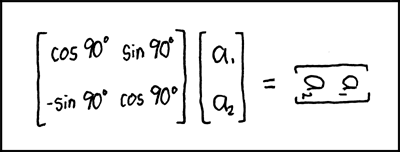
\includegraphics[width=0.5\textwidth]{Chapter1/images/XKCDmatrix_transform.png} \\{\small \textit{https://xkcd.com/184}}
    \end{center}
    }
    \vfill 
}








% \frame{\frametitle{Example: Constructing a Standard Matrix}

%     Define a linear transformation by $$ T (x_1 ,x_2) = (3x_1 + x_2 , 5x_1 + 7 x_2 , x_1 + 3 x_2 )$$ Is $T$ one-to-one?  Is $T$ onto?  



% }

\frame{\frametitle{Summary}

    \SummaryLine \vspace{4pt}
    \begin{itemize}\setlength{\itemsep}{8pt}
            \item standard vectors $\vec e_i$
            \item construct the standard matrix of a linear transform in $\mathbb R^n$ using the result that $A = \begin{pmatrix}
        T (\vec e_1) & T(\vec e_2)  & \cdots  & T (\vec e_n)
    \end{pmatrix}$
            \item constructing the standard matrix for a rotation matrix
    \end{itemize}
    \vspace{12pt}
    Note that
    \begin{itemize}
        \item The rotation matrix was just one of many standard matrices that are introduced in introductory linear algebra textbooks.
        \item There are other standard matrices for transformations that we will explore.
    \end{itemize}
}


 % REDOING
    % \title{Standard Matrices of Linear Transforms} 
\subtitle{\SubTitleName}
\institute[]{\Course}
\author{\Instructor}
\maketitle   

\frame{\frametitle{Topics and Learning Objectives}

\Emph{Topics} \\

\TopicStatement

\begin{itemize}
    \item the \Emph{standard vectors} and the \Emph{standard matrix}
    \item two dimensional transformations in more detail
    % \item \Emph{Onto} and \Emph{one-to-one} transformations. 
\end{itemize}

\vspace{0.5cm}
    
    \LO\\
    
    \LearningObjectiveStatement
    
    \begin{itemize}
        \item identify and construct linear transformations of a matrix
        % \item Characterize linear transformations as onto and/or one-to-one. 
        % \item Solve linear systems represented as linear transforms.
        % \item Express linear transforms in other forms, such as as matrix equations or as vector equations.
    \end{itemize}



\vspace{0.25cm} 

%\Emph{Motivating Question} \\

%A linear transformation  $ T \;:\;  \mathbb R ^2 \mapsto \mathbb R ^{3} $  satisfies 
%\begin{equation*}
%T \begin{pmatrix} 1 \\ 0 \end{pmatrix} = \begin{pmatrix} 5 \\ -7 \\ 2  \end{pmatrix},
%\qquad 
%T \begin{pmatrix*}[r]  0 \\ 1 \end{pmatrix*} = \begin{pmatrix*}[r] -3 \\ 8 \\ 0  
%\end{pmatrix*}
%\end{equation*}
%Is there a matrix that represents $ T_A$? If so, what could it be equal to? 
}






% \frame{\frametitle{Definition: The Standard Vectors}

%     The \Emph{standard vectors} in $\mathbb R^n$ are the vectors $\vec e_1, \vec e_2, \ldots , \vec e_n$, where: 
    
%     $$\vec e_1 = \hspace{2cm} \vec e_2 = \hspace{2cm} \vec e_n = $$
    
%     \vspace{2cm} 
    
%     For example, in $\mathbb R^3$, 
    
%         $$\vec e_1 = \hspace{2cm} \vec e_2 = \hspace{2cm} \vec e_3 = $$

% } 


% \frame{\frametitle{A Property of the Standard Vectors}

%     \Emph{Note}: if $A$ is an $m\times n$ matrix with columns $\vec v_1,\vec v_2,\ldots, \vec v_n$, then
%     $$A\vec e_i = \vec v_i, \text{ for } i=1,2,\ldots,n$$
%     So multiplying a matrix by $\vec e_i$ gives column $i$ of $A$.\\[6pt]

%     \Emph{Example}\\
%     $$\spalignmat{1 2 3; 4 5 6; 7 8 9} \vec e_2 = \hspace{6cm} $$

    
% }




% \frame{\frametitle{The Standard Matrix}

% \begin{center}\begin{tikzpicture} \node [mybox](box){\begin{minipage}{0.80\textwidth} 

%     Let $  T \;:\;  \mathbb R ^n \mapsto \mathbb R ^m $ be a linear transformation.  
%     Then there is a unique matrix $ A$ such that 
%     \begin{equation*}
%         T ( \vec x ) = A \vec x, \qquad \vec x\in \mathbb R ^{n}. 
%     \end{equation*}
%     In fact, $ A$ is a $ m \times n$, and its $ j^{th}$ column is the vector $ T (\vec e _j)$.  
%     \begin{equation*}
%         A = \begin{pmatrix}
%         T (\vec e_1) & T(\vec e_2)  & \cdots  & T (\vec e_n)
%     \end{pmatrix}
%     \end{equation*}

%     \end{minipage}}; \node[fancytitle, right=10pt] at (box.north west) {Theorem}; \end{tikzpicture}\end{center}

%     The matrix $ A$ is the \Emph{standard matrix} for a linear transformation.

% }



% \frame{\frametitle{Rotations}

%     \Emph{Example 1} \\
%     What is the linear transform $T : \R^2 \rightarrow \R^2$ defined by 
%     \begin{center}
%         $T(\vec x) = \vec x \text{ rotated counterclockwise by angle } \theta$?
%     \end{center}


% }

\frame{\frametitle{Standard Matrices in $\mathbb R^2$}

    \begin{itemize}
        \item There is a long list of geometric transformations of $\R^2$ in our textbook, as well as on the next few slides
        (reflections, rotations, contractions and expansions, shears, projections, \ldots).
        \item Please familiarize yourself with them: you are expected to memorize them, or be able to derive them.
    \end{itemize}

}



\frame{\frametitle{Two Dimensional Examples: Reflections}
    \vspace{-16pt}
    {\small 
    \begin{center}
        \begin{tabular}{ p{4.5cm} p{4.0cm} p{3.5cm}}
        \hline
        \Emph{transformation} & \Emph{image of unit square} & \Emph{standard matrix} \\
        \hline 
        \vspace{2pt} reflection through $x_1-$axis & 
        \vspace{2pt} \begin{tikzpicture}[scale=0.8]

    \coordinate (O) at (0,0);  % variable for origin
    
    % grey box
        \filldraw[
        draw=black!80,fill=black!10]          
            (0,1) 
            -- (1,1)
            -- (1,0)
            -- (O)
            -- cycle;
            
    % blue box
        \filldraw[
        draw=DarkBlue!80,fill=Teal!30]          
            (1,0) 
            -- (1,-1)
            -- (0,-1)
            -- (O)
            -- cycle;      
    
    % axes
    \draw[-, thin,black] (-0.5,0) -- (2.5,0) node[anchor=north east] {$x_1$};
    \draw[-, thin,black] (0,-0.5) -- (0.0,1.75) node[anchor=east] {$x_2$};
    
    % coordinate vectors                
    \draw[->,Black,very thick,-stealth,rotate=0] (O) -- (0,1) node[anchor=north east] {$\vec e_2$}; 
    \draw[->,Black,very thick,-stealth,rotate=0] (O) -- (1,0) node[anchor=north west] {$\vec e_1$}; 
    
\end{tikzpicture} & 
        \vspace{2pt} $\spalignmat{1 0;0 -1}$
        \\
        \vspace{2pt} reflection through $x_2-$axis & 
        \vspace{2pt} \begin{tikzpicture}[scale=0.8]

    \coordinate (O) at (0,0);  % variable for origin
       
    % grey box
        \filldraw[
        draw=black!80,fill=black!10]          
            (0,1) 
            -- (1,1)
            -- (1,0)
            -- (O)
            -- cycle;
            
    % blue box
        \filldraw[
        draw=DarkBlue!80,fill=Teal!30]          
            (-1,0) 
            -- (-1,1)
            -- (0,1)
            -- (O)
            -- cycle;            
    % axes
    \draw[-, thin,black] (-1.25,0) -- (1.5,0) node[anchor=west] {$x_1$};
    \draw[-, thin,black] (0,-0.5) -- (0.0,1.75) node[anchor=east] {$x_2$};
    
    % coordinate vectors            
    \draw[->,Black,very thick,-stealth,rotate=0] (O) -- (0,1) node[anchor=north east] {$\vec e_2$}; 
    \draw[->,Black,very thick,-stealth,rotate=0] (O) -- (1,0) node[anchor=north] {$\vec e_1$}; 
    
\end{tikzpicture} & 
        \vspace{2pt} $\spalignmat{-1 0;0 1}$
        \\        
        \end{tabular}
    \end{center}
    }
}

\frame{\frametitle{Two Dimensional Examples: Reflections}
    \vspace{-16pt}
    {\small 
    \begin{center}
        \begin{tabular}{ p{4.5cm} p{4.0cm} p{3.5cm}}
        \hline
        \Emph{transformation} & \Emph{image of unit square} & \Emph{standard matrix} \\
        \hline 
        \vspace{2pt} reflection through $x_2=x_1$ & 
        \vspace{2pt} 
        \begin{tikzpicture}[scale=0.8]

    \coordinate (O) at (0,0);  % variable for origin
       
    % grey and blue box
        \filldraw[
        draw=DarkBlue!80,fill=Teal!30]          
            (1,0) 
            -- (1,1)
            -- (0,1)
            -- (O)
            -- cycle;
            
          
    % axes
    \draw[-, thin,black] (-1.25,0) -- (1.5,0) node[anchor=west] {$x_1$};
    \draw[-, thin,black] (0,-0.5) -- (0.0,1.75) node[anchor=east] {$x_2$};
    
    % reflection line
    \draw[-,thin,Teal](-1,-1)--(1.2,1.2) node[anchor=south] {$x_2=x_1$};
    
    % coordinate vectors            
    \draw[->,Black,very thick,-stealth,rotate=0] (O) -- (0,1) node[anchor=north east] {$\vec e_2$}; 
    \draw[->,Black,very thick,-stealth,rotate=0] (O) -- (1,0) node[anchor=north] {$\vec e_1$}; 
    
\end{tikzpicture}&
        \vspace{2pt} $\spalignmat{0 1;1 0}$
        \\
        \vspace{2pt} reflection through $x_2=-x_1$ & 
        \vspace{2pt} 
        \begin{tikzpicture}[scale=0.8]

    \coordinate (O) at (0,0);  % variable for origin
       
    % grey box
        \filldraw[
        draw=black!80,fill=black!10]          
            (1,0) 
            -- (1,1)
            -- (0,1)
            -- (O)
            -- cycle;
            
    % blue box
        \filldraw[
        draw=DarkBlue!80,fill=Teal!30]          
            (-1,0) 
            -- (-1,-1)
            -- (0,-1)
            -- (O)
            -- cycle;            
    % axes
    \draw[-, thin,black] (-1.25,0) -- (1.5,0) node[anchor=west] {$x_1$};
    \draw[-, thin,black] (0,-0.5) -- (0.0,1.75) node[anchor=east] {$x_2$};
     \draw[-,thin,Teal](1,-1)--(-1,1)
    node[anchor=south] {$x_2=-x_1$};
    % coordinate vectors            
    \draw[->,Black,very thick,-stealth,rotate=0] (O) -- (0,1) node[anchor=north east] {$\vec e_2$}; 
    \draw[->,Black,very thick,-stealth,rotate=0] (O) -- (1,0) node[anchor=north] {$\vec e_1$}; 
    
\end{tikzpicture}&
        \vspace{2pt} $\spalignmat{0 -1;-1 0}$
        \\        
        \end{tabular}
    \end{center}
    }
}



\frame{\frametitle{Two Dimensional Examples: Contractions and Expansions}
    \vspace{-16pt}
    {\small 
    \begin{center}
        \begin{tabular}{ p{4.5cm} p{3.4cm} p{4cm}}
        \hline
        \Emph{transformation} & \Emph{image of unit square} & \Emph{standard matrix} \\
        \hline 
        \vspace{2pt} horizontal contraction & 
        \vspace{2pt} 
        \begin{tikzpicture}[scale=0.8]

    \coordinate (O) at (0,0);  % variable for origin

    % grey box
        \filldraw[
        draw=black!80,fill=black!10]          
            (0,1) 
            -- (1,1)
            -- (1,0)
            -- (O)
            -- cycle;
            
    % blue box
        \filldraw[
        draw=Teal!80,fill=Teal!30]          
            (0.5,0) 
            -- (0.5,1)
            -- (0,1)
            -- (O)
            -- cycle;            
    % axes
    \draw[-, thin,black] (-1.25,0) -- (1.5,0) node[anchor=west] {$x_1$};
    %\draw[., thin,black] (1,0) node[anchor=north]{$0<k<1$};
    \draw[-, thin,black] (0,-0.5) -- (0.0,1.75) node[anchor=east] {$x_2$};

    % coordinate vectors                
    \draw[->,Black,very thick,-stealth,rotate=0] (O) -- (0,1) node[anchor=north east] {$\vec e_2$}; 
    \draw[->,Black,very thick,-stealth,rotate=0] (O) -- (1,0) node[anchor=north west] {$\vec e_1$}; 
    
        
\end{tikzpicture}&
        \vspace{2pt} $\spalignmat{k 0;0 1}$. $|k|<1$
        \\
        \vspace{2pt} horizontal expansion & 
        \vspace{2pt} 
        \begin{tikzpicture}[scale=0.8]

    \coordinate (O) at (0,0);  % variable for origin
            
    % blue box
        \filldraw[
        draw=Teal!80,fill=Teal!30]          
            (1.4,0) 
            -- (1.4,1)
            -- (0,1)
            -- (O)
            -- cycle;            
    % axes
    \draw[-, thin,black] (-1.25,0) -- (1.5,0) node[anchor=west] {$x_1$};
    %\draw[.,thin,black] (1,0) node[anchor=north]{$k>1$};
    \draw[-, thin,black] (0,-0.5) -- (0.0,1.75) node[anchor=east] {$x_2$};
    
    % coordinate vectors                
    \draw[->,Black,very thick,-stealth,rotate=0] (O) -- (0,1) node[anchor=north east] {$\vec e_2$}; 
    \draw[->,Black,very thick,-stealth,rotate=0] (O) -- (1,0) node[anchor=north west] {$\vec e_1$}; 
        
\end{tikzpicture}&
        \vspace{2pt} $\spalignmat{k 0;0 1}$, $k>1$
        \\        
        \end{tabular}
    \end{center}
    }
}

\frame{\frametitle{Two Dimensional Examples: Contractions and Expansions}
    \vspace{-16pt}
    {\small 
    \begin{center}
        \begin{tabular}{ p{4.5cm} p{3.4cm} p{4cm}}
        \hline
        \Emph{transformation} & \Emph{image of unit square} & \Emph{standard matrix} \\
        \hline 
        \vspace{2pt} vertical contraction & 
        \vspace{2pt} 
        \begin{tikzpicture}[scale=0.8]

    \coordinate (O) at (0,0);  % variable for origin

    % grey box
        \filldraw[
        draw=black!80,fill=black!10]          
            (0,1) 
            -- (1,1)
            -- (1,0)
            -- (O)
            -- cycle;
         
    % blue box
        \filldraw[
        draw=DarkBlue!80,fill=Teal!30]          
            (1,0) 
            -- (1,0.5)
            -- (0,0.5)
            -- (O)
            -- cycle;            
    % axes
    \draw[-, thin,black] (-1.25,0) -- (1.5,0) node[anchor=west] {$x_1$};
    %\draw[., thin,black] (1,0) node[anchor=north]{$0<k<1$};
    \draw[-, thin,black] (0,-0.5) -- (0.0,1.75) node[anchor=east] {$x_2$};

    % coordinate vectors                
    \draw[->,Black,very thick,-stealth,rotate=0] (O) -- (0,1) node[anchor=north east] {$\vec e_2$}; 
    \draw[->,Black,very thick,-stealth,rotate=0] (O) -- (1,0) node[anchor=north west] {$\vec e_1$}; 
    
        
\end{tikzpicture}&
        \vspace{2pt} $\spalignmat{1 0;0 k}$, $|k|<1$
        \\
        \vspace{2pt} vertical expansion & 
        \vspace{2pt} 
        \begin{tikzpicture}[scale=0.8]

    \coordinate (O) at (0,0);  % variable for origin

    % blue box
        \filldraw[
        draw=DarkBlue!80,fill=Teal!30]          
            (1,0) 
            -- (1,1.4)
            -- (0,1.4)
            -- (O)
            -- cycle;                
    % grey box
        \filldraw[
        draw=black!80,fill=black!10]          
            (0,1) 
            -- (1,1)
            -- (1,0)
            -- (O)
            -- cycle;
            
        
    % axes
    \draw[-, thin,black] (-1.25,0) -- (1.5,0) node[anchor=west] {$x_1$};
    %\draw[.,thin,black] (1,0) node[anchor=north]{$k>1$};
    \draw[-, thin,black] (0,-0.5) -- (0.0,1.75) node[anchor=east] {$x_2$};
    
    % coordinate vectors                
    \draw[->,Black,very thick,-stealth,rotate=0] (O) -- (0,1) node[anchor=north east] {$\vec e_2$}; 
    \draw[->,Black,very thick,-stealth,rotate=0] (O) -- (1,0) node[anchor=north west] {$\vec e_1$}; 
    
        
\end{tikzpicture}&
        \vspace{2pt} $\spalignmat{1 0;0 k}$, $k>1$
        \\        
        \end{tabular}
    \end{center}
    }
}


\frame{\frametitle{Two Dimensional Examples: Shears}
    \vspace{-8pt}
    {\small 
    \begin{center}
        \begin{tabular}{ p{4.5cm} p{3.4cm} p{4cm}}
        \hline
        \Emph{transformation} & \Emph{image of unit square} & \Emph{standard matrix} \\
        \hline 
        \vspace{2pt} horizontal shear (left) & 
        \vspace{2pt} 
        \begin{tikzpicture}[scale=0.8]

    \coordinate (O) at (0,0);  % variable for origin

    % grey box
        \filldraw[
        draw=black!80,fill=black!10]          
            (0,1) 
            -- (1,1)
            -- (1,0)
            -- (O)
            -- cycle;
            
    % blue box
        \filldraw[
        draw=DarkBlue!80,fill=Teal!30]          
            (-0.5,1) 
            -- (0.5,1)
            -- (1,0)
            -- (O)
            -- cycle;            
    % axes
    \draw[-, thin,black] (-1.25,0) -- (1.5,0) node[anchor=west] {$x_1$};
    \draw[., thin,black] (1,0) node[anchor=north]{$k<0$};
    \draw[-, thin,black] (0,-0.5) -- (0.0,1.75) node[anchor=east] {$x_2$};
\end{tikzpicture}&
        \vspace{2pt} $\spalignmat{1 k;0 1}$, $k<0$
        \\
        \vspace{2pt} horizontal shear (right) & 
        \vspace{2pt} 
        \begin{tikzpicture}[scale=0.8]

    \coordinate (O) at (0,0);  % variable for origin

    % grey box
        \filldraw[
        draw=black!80,fill=black!10]          
            (0,1) 
            -- (1,1)
            -- (1,0)
            -- (O)
            -- cycle;
            
    % blue box
        \filldraw[
        draw=DarkBlue!80,fill=Teal!30]          
            (0.5,1) 
            -- (1.5,1)
            -- (1,0)
            -- (O)
            -- cycle;            
    % axes
    \draw[-, thin,black] (-1.25,0) -- (1.5,0) node[anchor=west] {$x_1$};
    \draw[., thin,black] (1,0) node[anchor=north]{$k>0$};
    \draw[-, thin,black] (0,-0.5) -- (0.0,1.75) node[anchor=east] {$x_2$};
\end{tikzpicture}&
        \vspace{2pt} $\spalignmat{1 k;0 1}$, $k>0$
        \\        
        \end{tabular}
    \end{center}
    }
}



\frame{\frametitle{Two Dimensional Examples: Shears}
    \vspace{-8pt}
    {\small 
    \begin{center}
        \begin{tabular}{ p{4.5cm} p{4.0cm} p{3.5cm}}
        \hline
        \Emph{transformation} & \Emph{image of unit square} & \Emph{standard matrix} \\
        \hline 
        \vspace{2pt} vertical shear (down) & 
        \vspace{2pt} 
        \begin{tikzpicture}[scale=0.8]

    \coordinate (O) at (0,0);  % variable for origin
    % grey box
        \filldraw[
        draw=black!80,fill=black!10]          
            (0,1) 
            -- (1,1)
            -- (1,0)
            -- (O)
            -- cycle;
            
    % blue box
        \filldraw[
        draw=DarkBlue!80,fill=Teal!30]          
            (0,1) 
            -- (1,0.5)
            -- (1,-0.5)
            -- (0,0)
            -- cycle;            
    % axes
    \draw[-, thin,black] (-1.25,0) -- (1.5,0) node[anchor=west] {$x_1$};
    %\draw[., thin,black] (1,-0.5) node[anchor=north]{$k<0$};
    \draw[-, thin,black] (0,-0.5) -- (0.0,1.75) node[anchor=east] {$x_2$};
    
    % coordinate vectors                
    \draw[->,Black,very thick,-stealth,rotate=0] (O) -- (0,1) node[anchor=north east] {$\vec e_2$}; 
    \draw[->,Black,very thick,-stealth,rotate=0] (O) -- (1,0) node[anchor=north west] {$\vec e_1$}; 
    
        
\end{tikzpicture}&
        \vspace{2pt} $\spalignmat{1 0;k 1}$, $k<0$
        \\
        \vspace{2pt} vertical shear (up) & 
        \vspace{2pt} 
        \begin{tikzpicture}[scale=0.8]

    \coordinate (O) at (0,0);  % variable for origin

    % grey box
        \filldraw[
        draw=black!80,fill=black!10]          
            (0,1) 
            -- (1,1)
            -- (1,0)
            -- (O)
            -- cycle;
            
    % blue box
        \filldraw[
        draw=DarkBlue!80,fill=Teal!30]          
            (0,1) 
            -- (1,1.5)
            -- (1,0.5)
            -- (0,0)
            -- cycle;            
    % axes
    \draw[-, thin,black] (-1.25,0) -- (1.5,0) node[anchor=west] {$x_1$};
    %\draw[., thin,black] (1,0) node[anchor=north]{$k>0$};
    \draw[-, thin,black] (0,-0.5) -- (0.0,1.75) node[anchor=east] {$x_2$};
    
    % coordinate vectors                
    \draw[->,Black,very thick,-stealth,rotate=0] (O) -- (0,1) node[anchor=north east] {$\vec e_2$}; 
    \draw[->,Black,very thick,-stealth,rotate=0] (O) -- (1,0) node[anchor=north west] {$\vec e_1$}; 
    
        
\end{tikzpicture}&
        \vspace{2pt} $\spalignmat{1 0;k 1}$, $k>0$
        \\        
        \end{tabular}
    \end{center}
    }
}



\frame{\frametitle{Two Dimensional Examples: Projections}
    \vspace{-8pt}
    {\small 
    \begin{center}
        \begin{tabular}{ p{4.5cm} p{4.0cm} p{3.5cm}}
        \hline
        \Emph{transformation} & \Emph{image of unit square} & \Emph{standard matrix} \\
        \hline 
        \vspace{2pt} projection onto the $x_1$-axis & 
        \vspace{2pt} 
        \begin{tikzpicture}[scale=0.8]

    \coordinate (O) at (0,0);  % variable for origin
    
    % grey box
        \filldraw[
        draw=black!80,fill=black!10]          
            (0,1) 
            -- (1,1)
            -- (1,0)
            -- (O)
            -- cycle;
    
    % blue box
        \filldraw[
        draw=DarkBlue!80,fill=Teal!40]          
            (0,.08) 
            -- (1,.08)
            -- (1,-.08)
            -- (0,-.08)
            -- cycle;            
            
  %\draw[-,yellow] (0,0.02) -- (1,0.02); 
  
    % axes
    \draw[-, thin,black] (-1.25,0) -- (1.5,0) node[anchor=west] {$x_1$};
    \draw[-, thin,black] (0,-0.5) -- (0.0,1.75) node[anchor=east] {$x_2$};
    
    % coordinate vectors                
    \draw[->,Black,very thick,-stealth,rotate=0] (O) -- (0,1) node[anchor=north east] {$\vec e_2$}; 
    \draw[->,Black,very thick,-stealth,rotate=0] (O) -- (1,0) node[anchor=north west] {$\vec e_1$}; 
        
\end{tikzpicture}&
        \vspace{2pt} $\spalignmat{1 0;0 0}$
        \\
        \vspace{2pt} projection onto the $x_2$-axis & 
        \vspace{2pt} 
        \begin{tikzpicture}[scale=0.8]

    \coordinate (O) at (0,0);  % variable for origin
            
    % grey box
        \filldraw[
        draw=black!80,fill=black!10]          
            (0,1) 
            -- (1,1)
            -- (1,0)
            -- (O)
            -- cycle;

    % blue box
        \filldraw[
        draw=DarkBlue!80,fill=Teal!30]          
            (0.08,0.00) 
            -- (0.08,1.00)
            -- (-0.08,1.00)
            -- (-0.08,0.00)
            -- cycle;      
            
  \draw[-,red] (0,0) -- (0,1);         
    % axes
    \draw[-, thin,black] (-1.25,0) -- (1.5,0) node[anchor=west] {$x_1$};
    \draw[-, thin,black] (0,-0.5) -- (0.0,1.75) node[anchor=east] {$x_2$};
    
    % coordinate vectors                
    \draw[->,Black,very thick,-stealth,rotate=0] (O) -- (0,1) node[anchor=north east] {$\vec e_2$}; 
    \draw[->,Black,very thick,-stealth,rotate=0] (O) -- (1,0) node[anchor=north west] {$\vec e_1$}; 
    
        
\end{tikzpicture}&
        \vspace{2pt} $\spalignmat{0 0;0 1}$
        \\        
        \end{tabular}
    \end{center}
    }
}






\frame{\frametitle{Example: Composite Transform}

Construct a matrix $A \in \mathbb R^{2\times 2}$, such that $T(\vec{x}) = A\vec{x}$, where $T$ is a linear transformation that rotates vectors in $\mathbb R^2$ counterclockwise by $\pi/2$ radians about the origin, then reflects them through the line $x_1 = x_2$.

}



\frame{\frametitle{Summary}

    \SummaryLine \vspace{4pt}
    \begin{itemize}\setlength{\itemsep}{8pt}
            \item constructing linear transformations in $\mathbb R^2$ and gave geometric interpretations for them
            \item constructing composite transform that involve two ore more linear transforms
    \end{itemize}

}

 
    %\title{Onto and One-to-One} 
\subtitle{\SubTitleName}
\institute[]{\Course}
\author{\Instructor}
\maketitle   

\frame{\frametitle{Topics and Learning Objectives}

\Emph{Topics} \\

\TopicStatement

\begin{itemize}
    % \item The \Emph{standard vectors} and the \Emph{standard matrix}.
    % \item Two and three dimensional transformations in more detail.  
    \item \Emph{onto} and \Emph{one-to-one} transformations
\end{itemize}

\vspace{0.5cm}
    
    \LO\\
    
    \LearningObjectiveStatement
    
    \begin{itemize}
        % \item Identify and construct linear transformations of a matrix.  
        \item characterize and construct linear transformations that are onto and/or one-to-one
        % \item Solve linear systems represented as linear transforms.
        % \item Express linear transforms in other forms, such as as matrix equations or as vector equations.
    \end{itemize}



\vspace{0.25cm} 

}


\frame{\frametitle{Onto}
 
    \begin{center}\begin{tikzpicture} \node [mybox](box){\begin{minipage}{0.80\textwidth} \vspace{2pt}
        A linear transformation $ T \;:\; \mathbb R ^{n} \to \mathbb R ^{m} $ is \Emph{onto} if for all $ \vec b \in \mathbb R ^{m}$ there is a $ \vec x\in \mathbb R ^{n}$ so that $ T (\vec x) = A\vec x = \vec b$.  

    \end{minipage}}; \node[fancytitle, right=10pt] at (box.north west) {Definition}; \end{tikzpicture}\end{center}

    

    \vspace{0.25cm} 

    \Emph{Implications}

    \begin{itemize}

        \item Onto is an \Emph{existence property:} for any $ \vec b \in \mathbb R ^{m}$, $ A \vec x = \vec b$ has a solution. 

        \item $T$ is onto if and only if its standard matrix has a pivot in every row.  

    \end{itemize}


}






\frame{\frametitle{One-to-One}

\begin{center}\begin{tikzpicture} \node [mybox](box){\begin{minipage}{0.90\textwidth} \vspace{2pt}
 A linear transformation $ T \;:\; \mathbb R ^{n} \to \mathbb R ^{m} $ is \Emph{one-to-one}  
 if 
 for all $ \vec b \in \mathbb R ^{m}$ there is at most one (possibly no) $ \vec x\in \mathbb R ^{n}$ so that $ T\left( \vec x \right)= A\vec x = \vec b$.  

 \end{minipage}}; \node[fancytitle, right=10pt] at (box.north west) {Definition}; \end{tikzpicture}\end{center}


\vspace{0.25cm} 

\Emph{Implications}

%%  ENUMERATE
\begin{itemize}
        \item One-to-one is a uniqueness property, it does not assert existence for all $\vec b$.

        \item $ T$ is one-to-one if and only if the only solution to $ T \left( \vec x \right) = \vec 0$ is the zero vector, $ \vec x = \vec 0$. 
        
        \item  $ T$ is one-to-one if and only if every column of $A$ is pivotal.
\end{itemize}


}


\frame{\frametitle{Example: Matrix Completion, One-to-one and Onto}

    Complete the matrices by entering numbers into the missing entries so that the properties are satisfied. \Emph{If it isn't possible to do so, state why}.
    \begin{enumerate}[a)]
            \item $A$ is a $2\times3$ standard matrix for a one-to-one transform. $$A = \spalignmat{1 , 0, ; 0, , 1}$$
            % \item $B$ is a $3\times2$ standard matrix for an onto transform.  $B = \spalignmat{1 , ; ,; ,}$ 
            \item $B$ is a $3\times3$ standard matrix for a transform that is one-to-one and onto.  $$B = \spalignmat{1,1,1; ;,,;,,}$$
    \end{enumerate}

}



\frame{\frametitle{Theorem for Onto Transforms}

    \begin{center}\begin{tikzpicture} \node [mybox](box){\begin{minipage}{0.80\textwidth} \vspace{2pt}
    For a linear transformation $ T \;:\; \mathbb R ^{n} \to \mathbb R ^{m}$ with standard matrix $ A$, these are equivalent statements.  
    %%  ENUMERATE
    \begin{enumerate}
    \item  $ T$ is onto. 
    
    \item $ A$ has  columns that span $ \mathbb R ^{m}$. 
    
    \item Every row of $A$ is pivotal.  
    \end{enumerate}
    %% ENUMERATE
    
    \end{minipage}}; \node[fancytitle, right=10pt] at (box.north west) {Theorem}; \end{tikzpicture}\end{center}


}

\frame{\frametitle{Theorem for One-to-one Transforms}

    \begin{center}\begin{tikzpicture} \node [mybox](box){\begin{minipage}{0.80\textwidth} \vspace{2pt}
    For a linear transformation $ T \;:\; \mathbb R ^{n} \to \mathbb R ^{m}$ with standard matrix $ A$, these are equivalent statements.  
    
    \begin{enumerate}
    \item  $ T$ is one-to-one. 
    
    \item The unique solution to $ T \left( \vec x \right) = \vec 0$ is the trivial one. 
    
    \item $A$ has linearly independent columns.  
    
    \item Each column of $A $ is pivotal.  
    \end{enumerate}
    
    
    \end{minipage}}; \node[fancytitle, right=10pt] at (box.north west) {Theorem}; \end{tikzpicture}\end{center}


}

\frame{\frametitle{Example: Constructing a Standard Matrix, One-to-one \\and Onto}

    Define a linear transformation by $$ T (x_1 ,x_2) = (3x_1 + x_2 , 5x_1 + 7 x_2 , x_1 + 3 x_2 )$$ Construct the standard matrix for the transformation. Is $T$ one-to-one?  Is $T$ onto?  


}




\frame{\frametitle{Example: Linear Transform Review}

    Suppose $A$ is an $m \times n$ standard matrix for transform $T$, and there are some vectors $\vec b \in \mathbb R^m$ that are not in the range of $T(\vec x) = A\vec x$. 
    
    
     
    
    True or false:
    \begin{enumerate}
        \item $A\vec x = \vec b$ could be inconsistent
        \item there cannot be a pivot in every column of $A$
        \item $T$ could be one-to-one
    \end{enumerate}


}



\frame{\frametitle{Summary}

    \SummaryLine \vspace{4pt}
    \begin{itemize}\setlength{\itemsep}{8pt}
            \item constructing linear transformations of a matrix that are one-to-one and/or onto 
            \item characterizing transforms that are one-to-one/onto
    \end{itemize}
    
}

 
% \fi 


%%%%%%%%%%%
% MODULE 2

% \ifnum \Week = 4
    % \renewcommand{\SubTitleName}{Matrix Algebra}
    % \title{Matrix Addition and Scalar Multiplication}
\subtitle{\SubTitleName}
\institute[]{\Course}
\author{\Instructor}
\maketitle   


\tikzstyle{startstop} =[trapezium, trapezium left angle=70, trapezium right angle=110, minimum width=1cm, minimum height=1cm, text centered, fill=Teal!30]

\tikzstyle{io} = [trapezium, trapezium left angle=70, trapezium right angle=110, minimum width=1cm, minimum height=1cm, text centered, fill=DarkRed!30]

\tikzstyle{process} = [trapezium, trapezium left angle=70, trapezium right angle=110, minimum width=1cm, minimum height=1cm, text centered, fill=Gold!60]

\tikzstyle{arrow} = [thick,->,>=stealth]

\frame{\frametitle{Topics and Objectives}
    \Emph{Topics} \\
    \TopicStatement
    \begin{itemize}
    
        \item identity and zero matrices
        
        \item matrix algebra: sums and scalar multiplies
        
    \end{itemize}
    
    \vspace{0.5cm}
    
    \Emph{Objectives}\\
    
    \LearningObjectiveStatement
    
    \begin{itemize}
    
        \item apply matrix algebra and the zero and identity matrices to solve and analyze matrix equations

    \end{itemize}


}



\frame{\frametitle{Definitions: Zero and Identity Matrices}

    \begin{itemize}

    \item A \Emph{zero matrix} is any matrix whose every entry is zero. 
    
    \begin{equation*}
        0_{2 \times 3} = 
        \begin{pmatrix}
            0 & 0 & 0\\ 0 & 0 & 0
        \end{pmatrix}
        , \quad 
        0_{2 \times 1} = 
        \begin{pmatrix}
            0 \\ 0
        \end{pmatrix}
    \end{equation*}    
    
    \pause 
    
    \item  The $n\times n$ \Emph{identity matrix} has ones on the main diagonal, otherwise all zeros. 
    \begin{equation*}
        I _{2} = 
        \begin{pmatrix}
            1 & 0 \\ 0 & 1 
        \end{pmatrix}
        , \quad 
        I _{3} = 
        \begin{pmatrix}
            1 & 0 & 0 \\ 0 & 1 & 0 \\ 0 & 0 & 1 
        \end{pmatrix}
    \end{equation*}
    
    \end{itemize}
    
    \pause 

    Note: any matrix with dimensions $n\times n$ is \Emph{square}. Zero matrices need not be square, identity matrices must be square. 

}

\begin{frame}
\frametitle{Matrix Addition and Scalar Multiples}

Suppose $ A$ and $B $ are $ m \times n$ matrices. \pause $a _{i,j}$ is the entry of $A$ in row $i$ and column $j$, and \pause $b _{i,j}$ is the entry of $B$ in row $i$ and column $j$. 

\begin{itemize}

    \item The entries of $ A+B$ are $a_{i,j} + b_{i,j}$. 

    \item If $ c \in \mathbb R$, then the entries of $c A$ are $c a _{i,j}$.  

\end{itemize}
\pause 
For example, if 

$$
\begin{pmatrix} 1 & 2 & 3 \\ 4 & 5 & 6 \end{pmatrix} + c
\begin{pmatrix} 7 & 4 & 7 \\ 0 & 0 & k \end{pmatrix} =
\begin{pmatrix} 15 & 10 & 17 \\ 4 & 5 & 16 \end{pmatrix}
$$
What are the values of $c$ and $k$?

\end{frame}





\frame{\frametitle{Properties of Sums and Scalar Multiples}

Scalar multiples and matrix addition have the expected properties. \\[12pt] If $ r, s \in \mathbb R $ are scalars, and $ A, B, C$ are $ m \times n$ matrices, then 
%%  ENUMERATE
\begin{enumerate}
\item<1->  $ A + 0 _{m \times n} = A$
\item<2->  $ (A+B) + C = A + (B+C)$
\item<3-> $ r (A+B) = r A + r B $ 
\item<4-> $ (r+s) A = r A + s A $ 
\item<5->  $ r (sA) = (rs) A$ 
\end{enumerate}
%% ENUMERATE

}


\frame{\frametitle{Summary}

    \SummaryLine \vspace{4pt}
    \begin{itemize}\setlength{\itemsep}{8pt}
        \item the identity and zero matrices
        \item matrix algebra: sums and scalar multiplies
    \end{itemize}
    \vspace{4pt}
    % There are several ways of multiplying matrices that we explore in this class. This video introduced two methods. 
}




% \frame{\frametitle{Matrix Multiplication}


% \begin{center}\begin{tikzpicture} \node [mybox](box){\begin{minipage}{0.80\textwidth}

% Let $ A $ be a $ m \times n $ matrix, and $ B$ be a $ n \times p$ matrix. The product is  $ A B  $ a $ m \times p$ matrix, equal to $$ A B = A 
% \begin{pmatrix}
% \vec b_1 & \cdots & \vec b_p
% \end{pmatrix} = 
% \begin{pmatrix}
% A \vec b_1 & \cdots & A \vec b_p
% \end{pmatrix}
% $$ 
% \end{minipage}};
% \node[fancytitle, right=10pt] at (box.north west) {Definition};
% \end{tikzpicture}\end{center}

%     \Emph{Example} \\
    
%     Compute the following product. 
    
%     \begin{equation*}
%     C = AB = 
%     \spalignmat{2 0;1 1}\spalignmat{2 0 0;3 4 0}
%     \end{equation*}

% }


% \frame{\frametitle{Row Column Rule for Matrix Multiplication }

%     The Row Column Rule is a convenient way to calculate the product $AB$ that many students have encountered in pre-requisite courses. 
    
%     \begin{center}\begin{tikzpicture} \node [mybox](box){\begin{minipage}{0.80\textwidth}
    
%     If $A \in \mathbb R^{m\times n}$ has rows $\vec a_i$, and $B \in \mathbb R^{n \times p}$ has columns $\vec b_j$, each element of the product $C=AB$ is the dot product $c_{ij} = \vec a_i \cdot \vec b_j$.
%     \end{minipage}};
%     \node[fancytitle, right=10pt] at (box.north west) {Row Column Method};
%     \end{tikzpicture}\end{center}
    
%     \Emph{Example} \\
    
%     Compute the following using the row-column method. 
    
%     \begin{equation*}
%     C = AB = 
%     \spalignmat{2 0;1 1}\spalignmat{2 0 0;3 4 0}
%     \end{equation*}


% }

% \frame{\frametitle{Matrix Dimensions and Matrix Multiplication}

%     Note: the dimensions of $A$ and $B$ determine whether $AB$ is defined, and what its dimensions will be.
    
%     \begin{center}
%         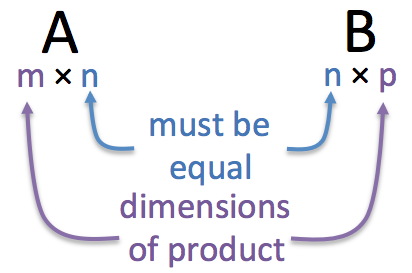
\includegraphics[width=0.3\textwidth]{Chapter2/images/matrix_multi2} 
%     \end{center}

% }



% \frame{\frametitle{Properties of Matrix Multiplication} 

%     Let $ A, B, C$ be matrices of the sizes needed for the matrix multiplication to be defined, and $ A $ is a $ m \times n$ matrix. 
    
%     \begin{enumerate}
%         \item (Associative)  $(AB)C= A (BC)$ 
%         \item (Left Distributive)  $A (B+C) = AB + AC $ 
%         \item (Right Distributive) $(A + B)C = AC + AC $ 
%         \item (Identity for matrix multiplication)  $ I _{m} A = A I _{n}$ 
%     \end{enumerate}

    
%     \Emph{\color{Teal}Warnings:}  
%     \begin{enumerate}
%         \item  (non-commutative)    In general, $ AB \neq BA $.   
%         \item  (non-cancellation)  $ AB = A C $ does not mean $ B=C$. 
%         \item  (Zero divisors)   $ AB = 0$ does not mean that either $ A=0$ or $ B=0$.  
%     \end{enumerate}

% }

% \frame{\frametitle{Examples}
%     Suppose $A = \spalignmat{1 0; 0 0}$.
%     \begin{enumerate}
%         \item Give an example of a $2\times2$ matrix that does not commute with $A$. 
%         \item Construct any non-zero matrices $B$ and $C$ so that $B\ne C$ but $AB=BC$.
%     \end{enumerate}
    
% }


% \frame{\frametitle{The Associative Property} 

%     If $C = \vec x$, then the associative property is: $(AB)\vec x = A (B \vec x)$. Schematically: 
    
%     \vspace{18pt}
    
%     \begin{tikzpicture}[node distance=2cm]

%         \node(x)  [startstop] {$\vec x$};
%         \node(bx) [io, below of=x] {$B\vec x$};
%         \node(abx)[process, right of=x,xshift=4cm]{$AB\vec x$};
        
%         \draw [arrow] (x) -- node[anchor=east] {\small Multiplication by $B$} (bx);
%         \draw [arrow] (bx) -- node[anchor=north,xshift=1.2cm] {\small Multiplication by $A$} (abx);
%         \draw [arrow] (x) --node[anchor=south] {\small  \ \ \ Multiplication by $AB$} (abx);
        
%     \end{tikzpicture}

%     \vspace{4pt}

%     The matrix product $ AB\vec x$ can be obtained by either: multiplying by matrix $AB$, or by multiplying by $B$ then by $A$. This means that matrix multiplication corresponds to \Emph{composition of the linear transformations}.
% }

% % 


% % \begin{frame}
% % \frametitle{Additional Examples}

% %     True or false:

% %     \begin{enumerate}
% %         \item For any $I_n$ and any $A \in \R^{n\times n}$, $(I_n + A)(I_n - A) = I_n - A^2$. \\[3cm]
% %         \item For any $A$ and $B$ in $\R^{n\times n}$, $(A+B)^2 = A^2 + B^2 + 2AB$. 
% %     \end{enumerate}

% % \end{frame}

% \frame{\frametitle{Summary}

%     \SummaryLine \vspace{4pt}
%     \begin{itemize}\setlength{\itemsep}{8pt}
%         \item the identity and zero matrices
%         \item matrix algebra: sums and products, scalar multiplies
%     \end{itemize}
%     \vspace{4pt}
%     There are several ways of multiplying matrices that we explore in this class. This video introduced two methods. 
% }

    % \title{Matrix Multiplication}
\subtitle{\SubTitleName}
\institute[]{\Course}
\author{\Instructor}
\maketitle

\tikzstyle{startstop} =[trapezium, trapezium left angle=70, trapezium right angle=110, minimum width=1cm, minimum height=1cm, text centered, fill=Teal!100]

\tikzstyle{io} = [trapezium, trapezium left angle=70, trapezium right angle=110, minimum width=1cm, minimum height=1cm, text centered, fill=DarkRed]

\tikzstyle{process} = [trapezium, trapezium left angle=70, trapezium right angle=110, minimum width=1cm, minimum height=1cm, text centered, fill=Gold!100]

\tikzstyle{arrow} = [thick,->,>=stealth]

\frame{\frametitle{Motivation}

    Suppose we need a linear transform of the form $T(\vec x) = A\vec x$, \onslide<2->{but $A$ is a combination of many transforms. For example: }
    \begin{align*}
        \onslide<3->{A = }\onslide<4->{\underbrace{\begin{pmatrix}
            0&-1 \\ 1&0
        \end{pmatrix}}_{rotation}}\onslide<5->{
        \underbrace{\begin{pmatrix}
            2&0 \\ 0&2
        \end{pmatrix}}_{dilation}}\onslide<6->{
        \underbrace{\begin{pmatrix}
            0&1 \\ 1&0
        \end{pmatrix}}_{reflection}
        \cdots}
    \end{align*}
    \pause 
    \onslide<7->{How can we calculate the product of two (or more) matrices? How does multiplying matrices compare to multiplying numbers? }\onslide<8->{What is matrix multiplication? }

    \vspace{12pt}
    
    \onslide<9->{
    \Emph{Objectives}\\
    \LearningObjectiveStatement \ multiply two matrices together. }    
}


% % First slide - Definition (keeping the original)
% \frame{\frametitle{Matrix Multiplication}
% \vspace{-12pt}
% \begin{center}\begin{tikzpicture} \node [mybox](box){\begin{minipage}{0.95\textwidth}
%     Let $ A $ be an $ m \times n $ matrix, and $ B$ be an $ n \times p$ matrix. \onslide<2->{ The product  $ A B  $ is an $ m \times p$ matrix,} \onslide<3->{equal to} \onslide<3->{$$ A B = A 
%     \begin{pmatrix}
%     \vec b_1 & \cdots & \vec b_p
%     \end{pmatrix} = \onslide<4->{
%     \begin{pmatrix}
%     A \vec b_1 & \cdots & A \vec b_p
%     \end{pmatrix}}
%     $$ }
%     \end{minipage}};
%     \node[fancytitle, right=10pt] at (box.north west) {Definition};
%     \end{tikzpicture}\end{center}
% }

\frame{\frametitle{Definition: Matrix Multiplication}

\vspace{-12pt}
\begin{center}\begin{tikzpicture} \node [mybox](box){\begin{minipage}{0.95\textwidth}

    Let $ A $ be an $ m \times n $ matrix, and $ B$ be an $ n \times p$ matrix. \onslide<2->{ The columns of $B$ are $\vec b_1, \vec b_2 , \cdots ,\vec b_p$. }\onslide<3->{The product  $ A B  $ is an $ m \times p$ matrix,} \onslide<4->{equal to} \onslide<5->{$$ A B = A 
    \begin{pmatrix}
    \vec b_1 & \cdots & \vec b_p
    \end{pmatrix} = 
    \begin{pmatrix}A \vec b_1 & \cdots & A \vec b_p\end{pmatrix}$$} \vspace{-16pt}
    \end{minipage}};
    \node[fancytitle, right=10pt] at (box.north west) {Definition};
    \end{tikzpicture}\end{center}

    \begin{itemize}
        \item<5-> You can think of matrix multiplication $AB$ as \onslide<6->{transforming the columns of $B$ according to a transform defined by $A$. }
        \item<7-> You may encounter other definitions in other textbooks and websites. Our definition is used later on for other theorems and procedures.  
        \item<8-> The above definition calculates the product column-by-column.         
    \end{itemize}
    % \onslide<5->{
    % \Emph{Example} \\
    
    % Compute the product. 
    
    % \begin{equation*}
    % C = AB = 
    % \spalignmat{2 0;1 1}\spalignmat{2 0 0;3 4 0}
    % \end{equation*}
    % }

}

\frame{\frametitle{Example Using the Definition}
    We want to compute
    \begin{equation*}
    C = AB = 
    \spalignmat{2 0;1 1}\spalignmat{2 0 0;3 4 0}
    \end{equation*}
    \onslide<2->{The result is a $2\times 3$ matrix, $C = \begin{pmatrix} \vec c_1 & \vec c_2 & \vec c_3\end{pmatrix}$.}
    \onslide<3->{So }
    \begin{align*}
        \onslide<3->{\vec c_1 &= A\begin{pmatrix} 2\\3\end{pmatrix} } \onslide<6->{= 2\begin{pmatrix} 2\\1\end{pmatrix}+3\begin{pmatrix} 0\\1\end{pmatrix}=}\onslide<7->{\begin{pmatrix} 4\\2\end{pmatrix} + \begin{pmatrix} 0\\3\end{pmatrix}}\onslide<8->{=\begin{pmatrix} 4\\5\end{pmatrix}}\\
        \onslide<4->{\vec c_2 &= A\begin{pmatrix} 0\\4\end{pmatrix} }\onslide<9->{= 0\begin{pmatrix} 2\\1\end{pmatrix}+4\begin{pmatrix} 0\\1\end{pmatrix}=\begin{pmatrix} 0\\0\end{pmatrix} + \begin{pmatrix} 0\\4\end{pmatrix}=\begin{pmatrix} 0\\4\end{pmatrix}}\\
        \onslide<5->{\vec c_3 &= A\begin{pmatrix} 0\\0\end{pmatrix} }\onslide<10->{= 0\begin{pmatrix} 2\\1\end{pmatrix}+0\begin{pmatrix} 0\\1\end{pmatrix}=\begin{pmatrix} 0\\0\end{pmatrix} + \begin{pmatrix} 0\\0\end{pmatrix}=\begin{pmatrix} 0\\0\end{pmatrix}}
    \end{align*}
}

\frame{\frametitle{Example Solution)}

    Final result: \pause
    $$C = AB = \begin{pmatrix} \vec c_1 & \vec c_2 & \vec c_3\end{pmatrix} = \begin{pmatrix} 4 & 0 & 0 \\ 5 & 4 & 0 \end{pmatrix}$$
    
}

\frame{\frametitle{Summary: Matrix Multiplication Definition}
\begin{itemize}
    \item<2-> The definition of matrix multiplication calculates the product column-by-column. 
    \item<3-> The definition also gives us insight into what matrix multiplication is: a transformation of the columns of one of the matrices. 
    \item<4-> You might be wondering: what other ways can we use to multiply matrices? 
    \item<5-> It turns out that not only are there many ways to multiply matrices together! And there is ongoing research on the best way to multiply matrices together! 
    \item<6-> We will introduce the row-column method for multiplying matrices, which calculates the product entry-by-entry. 
\end{itemize}
}

 % NEW
    % 
\title{The Row-Column Method for Matrix Multiplication}
\subtitle{\SubTitleName}
\institute[]{\Course}
\author{\Instructor}
\maketitle

\tikzstyle{startstop} =[trapezium, trapezium left angle=70, trapezium right angle=110, minimum width=1cm, minimum height=1cm, text centered, fill=Teal!100]

\tikzstyle{io} = [trapezium, trapezium left angle=70, trapezium right angle=110, minimum width=1cm, minimum height=1cm, text centered, fill=DarkRed]

\tikzstyle{process} = [trapezium, trapezium left angle=70, trapezium right angle=110, minimum width=1cm, minimum height=1cm, text centered, fill=Gold!100]

\tikzstyle{arrow} = [thick,->,>=stealth]

\frame{\frametitle{Motivation}

    \begin{itemize}
        \item <2-> The matrix multiplication definition calculates matrix products column-by-column. 
        \item <3-> The row-column method is commonly used for calculating matrix products by hand. 
        \item <4-> The row-column method calculates the product entry-by-entry. 
    \end{itemize} 

    \vspace{12pt}
    
    \onslide<5->{
    \Emph{Objectives}\\
    \LearningObjectiveStatement \ multiply matrices the row-column method. }    
}




\frame{\frametitle{Matrix Multiplication Using the Row-Column Method}
    Example: use the row-column method to compute
    \onslide<2->{
    \begin{equation*}
    C = A B = 
    \begin{pmatrix} 2 & 0 \\ 1 & 1 \end{pmatrix}
    \begin{pmatrix} 2 & 0 & 0 \\ 3 & 4 & 0 \end{pmatrix}
    \end{equation*}
    }
    
    \onslide<3->{
    \begin{itemize}
        \item<3-> The result $C$ will be the same matrix we calculated using the matrix multiplication definition. 
        \item<4-> We'll compute each entry using the row-column method.
        \item<5-> Highlighted rows and columns will show which numbers we're using.
    \end{itemize}
    }
}

% Computing first entry with highlighting
\frame{\frametitle{Computing $c_{11}$ (First Entry)}

    \begin{align}
        C = \begin{pmatrix}c_{11} & c_{12} & c_{13}\\c_{21} & c_{22} & c_{23} \end{pmatrix}=AB = \begin{pmatrix} \rowcolor{blue!10} 2 & 0 \\ 1 & 1 \end{pmatrix}
    \begin{pmatrix} \multicolumn{1}{>{\columncolor{green!10}}c}{2} & 0 & 0 \\ \multicolumn{1}{>{\columncolor{green!10}}c}{3} & 4 & 0 \end{pmatrix}
    \end{align}
    
    \pause
    And: 
    $$c_{11} = (2)(2) + (0)(3) = 4$$
    
    \pause
    
    \vspace{8pt}
    Result so far:
    
    \pause
    $$C = \begin{pmatrix} \mathbf{4} & ? & ? \\ ? & ? & ? \end{pmatrix}$$
}

% Computing second entry
\frame{\frametitle{Computing $c_{12}$}

    \begin{align}
    \begin{pmatrix} \rowcolor{blue!10} 2 & 0 \\ 1 & 1 \end{pmatrix}   \begin{pmatrix} 2 & \multicolumn{1}{>{\columncolor{green!10}}c}{0} & 0 \\ 3 & \multicolumn{1}{>{\columncolor{green!10}}c}{4} & 0 \end{pmatrix}
    \end{align}
    
    \pause
    And: 
    $$c_{12} = (2)(0) + (0)(4) = 0$$
    
    \vspace{8pt}
    \pause
    Result so far:
    $$C = \begin{pmatrix} 4 & \mathbf{0} & ? \\ ? & ? & ? \end{pmatrix}$$

}

% Computing third entry
\frame{\frametitle{Computing $c_{21}$}
    \begin{center}
    $\begin{pmatrix} 2 & 0 \\ \rowcolor{blue!10} 1 & 1 \end{pmatrix}$
    $\begin{pmatrix} \multicolumn{1}{>{\columncolor{green!10}}c}{2} & 0 & 0 \\ \multicolumn{1}{>{\columncolor{green!10}}c}{3} & 4 & 0 \end{pmatrix}$
    
    \vspace{8pt}
    $c_{21} = (1)(2) + (1)(3) = 5$
    
    \vspace{8pt}
    Result so far:
    $C = \begin{pmatrix} 4 & 0 & ? \\ \mathbf{5} & ? & ? \end{pmatrix}$
    \end{center}
}

% Computing fourth entry
\frame{\frametitle{Computing $c_{22}$ (Fourth Entry)}
    \begin{center}
    $\begin{pmatrix} 2 & 0 \\ \rowcolor{blue!10} 1 & 1 \end{pmatrix}$
    $\begin{pmatrix} 2 & \multicolumn{1}{>{\columncolor{green!10}}c}{0} & 0 \\ 3 & \multicolumn{1}{>{\columncolor{green!10}}c}{4} & 0 \end{pmatrix}$
    
    \vspace{8pt}
    $c_{22} = (1)(0) + (1)(4) = 4$
    
    \vspace{8pt}
    Result so far:
    $C = \begin{pmatrix} 4 & 0 & ? \\ 5 & \mathbf{4} & ? \end{pmatrix}$
    \end{center}
}

% Computing fifth and sixth entries
\frame{\frametitle{Computing Final Entries ($c_{13}$ and $c_{23}$)}
    \begin{center}
    For $c_{13}$:
    $\begin{pmatrix} \rowcolor{blue!10} 2 & 0 \\ 1 & 1 \end{pmatrix}$
    $\begin{pmatrix} 2 & 0 & \multicolumn{1}{>{\columncolor{green!10}}c}{0} \\ 3 & 4 & \multicolumn{1}{>{\columncolor{green!10}}c}{0} \end{pmatrix}$
    
    $c_{13} = (2)(0) + (0)(0) = 0$
    
    \vspace{8pt}
    For $c_{23}$:
    $\begin{pmatrix} 2 & 0 \\ \rowcolor{blue!10} 1 & 1 \end{pmatrix}$
    $\begin{pmatrix} 2 & 0 & \multicolumn{1}{>{\columncolor{green!10}}c}{0} \\ 3 & 4 & \multicolumn{1}{>{\columncolor{green!10}}c}{0} \end{pmatrix}$
    
    $c_{23} = (1)(0) + (1)(0) = 0$
    \end{center}

    \pause 
    Final result:
    $$C = AB = \begin{pmatrix} 4 & 0 & 0 \\ 5 & 4 & 0 \end{pmatrix}$$
    The same result obtained with the matrix multiplication definition.
    
}

% % Complete result
% \frame{\frametitle{Complete Matrix Multiplication}
%     \begin{center}
%     Final result:
    
%     \vspace{8pt}
%     \onslide<1->{
%     $C = AB = \begin{pmatrix} 4 & 0 & 0 \\ 5 & 4 & 0 \end{pmatrix}$
%     }
    
%     \vspace{12pt}
%     \onslide<2->{
%     \begin{tikzpicture} \node [mybox](box){\begin{minipage}{0.85\textwidth}
%     Each entry $c_{ij}$ is computed by:
%     \begin{itemize}
%         \item Taking row $i$ from matrix $A$ (highlighted in blue)
%         \item Taking column $j$ from matrix $B$ (highlighted in green)
%         \item Computing their dot product for entry $(i,j)$ in matrix $C$
%     \end{itemize}
%     \end{minipage}};
%     \node[fancytitle, right=10pt] at (box.north west) {Key Insight};
%     \end{tikzpicture}
%     }
%     \end{center}
% }

\frame{\frametitle{Theorem: The Row-Column Method}

\vspace{-12pt}
\begin{center}\begin{tikzpicture} \node [mybox](box){\begin{minipage}{0.95\textwidth}

    Let $ A $ be an $ m \times n $ matrix, and $ B$ be an $ n \times p$ matrix. \onslide<2->{ The entry in row $i$} \onslide<3->{and column $j$} \onslide<4->{of $AB$, is } \onslide<5->{the sum of the products of corresponding entries of row $i$ of $A$, and column $j$ of $B$. } \onslide<6->{That is, }
    $$\onslide<7->{(AB)_{ij} = } \onslide<8->{a_{i1}b_{1j} + }\onslide<9->{a_{i2}b_{2j} +}\onslide<10->{ a_{i3}b_{3j} + \cdots} \onslide<11->{+ a_{in}b_{nj}}$$ \vspace{-12pt}
    \end{minipage}};
    \node[fancytitle, right=10pt] at (box.north west) {Theorem};
    \end{tikzpicture}\end{center}

    \onslide<12->{\Emph{Brief explanation:} } \onslide<13->{Let $B = \begin{pmatrix}
        \vec b_1 & \vec b_2 & \cdots & \vec b_p\end{pmatrix}$. }\onslide<14->{Then by the definition of matrix multiplication, column $j$ of $AB$ is $A\vec b_j$. }\onslide<15->{ And entry $i$ of $A\vec b_j$ is found using the row-column rule.}

}


% Final summary slide
\frame{\frametitle{Summary}
    \begin{itemize}\setlength{\itemsep}{8pt}
        \item<2-> We have two ways to compute matrix multiplication: 
        \begin{itemize}
            \item {\normalsize the definition}
            \item {\normalsize the row-column method}
        \end{itemize}
        \item<3-> Often the row-column method is what we use for quick hand-calculations. 
        \item<4-> We use the definition when introducing new algorithms.
        \item<5-> There are many other ways of computing matrix products, but for now this is all we need. 
    \end{itemize}
} % NEW
    \title{Properties of Matrix Multiplication}
\subtitle{\SubTitleName}
\institute[]{\Course}
\author{\Instructor}
\maketitle


\tikzstyle{startstop} =[trapezium, trapezium left angle=70, trapezium right angle=110, minimum width=1cm, minimum height=1cm, text centered, fill=Teal!30]

\tikzstyle{io} = [trapezium, trapezium left angle=70, trapezium right angle=110, minimum width=1cm, minimum height=1cm, text centered, fill=DarkRed!30]

\tikzstyle{process} = [trapezium, trapezium left angle=70, trapezium right angle=110, minimum width=1cm, minimum height=1cm, text centered, fill=Gold!60]

\tikzstyle{arrow} = [thick,->,>=stealth]

\frame{\frametitle{Motivation}

    When $x$ and $y$ are real numbers, algebra can simplify equations that they involve. \pause For example: 
    \pause 
    \begin{itemize}
        \item If $xy=4y$ and $y\ne0$, then $x=4$. 
        \item For any real numbers $x$ and $y$, we can use $xy = yx$
    \end{itemize}
    \pause 
    Can we make similar statements with matrices? 
    \pause 

    \vspace{12pt}
    
    \Emph{Objectives}\\
        
    \begin{itemize}

        \item determine whether the multiplication of two matrices is defined

        \item apply algebraic properties of matrix multiplication to simplify and analyze matrix equations
        
    \end{itemize}


}

\frame{\frametitle{Matrix Dimensions and Matrix Multiplication}

    \pause The dimensions of $A$ and $B$ determine whether $AB$ is defined, \pause and what its dimensions will be.
    \pause 
    
    \begin{center}
        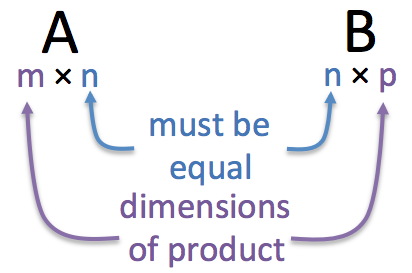
\includegraphics[width=0.3\textwidth]{Chapter2/images/matrix_multi2} 
    \end{center}

}


\frame{\frametitle{Example}

    Suppose $A$ is $3\times 5$ and $B$ is $5\times7$. Then:
    \begin{itemize}
        \item<2-> $AB$ is defined and the result is \onslide<3->{$3\times 7$}
        \item<4-> $BA$ is not defined \onslide<5->{because the number of columns of $B$ is not equal to the number of rows of $A$. }
    \end{itemize}

}


\frame{\frametitle{Properties of Matrix Multiplication} 

    \onslide<2->{$ A, B, C$ are matrices with sizes needed for matrix multiplication to be defined. }
    
    \begin{enumerate}
        \item<3-> (Associative)  $(AB)C= A (BC)$ 
        \item<4-> (Left Distributive)  $A (B+C) = AB + AC $ 
        \item<4-> (Right Distributive) $(A + B)C = AC + BC $ 
        \item<5-> (Identity)  $ I _{m} A = A I _{n}$, where $A$ is $m\times n$
    \end{enumerate}

    \onslide<6->{
    \Emph{\color{Teal}Warnings:}  
    }
    \begin{enumerate}
        \item<7->  (non-commutative) In general, $ AB \neq BA $. \pause  
        \item<8->  (non-cancellation) $ AB = A C $ does not mean $ B=C$. \pause 
        \item<9->  (Zero divisors) $ AB = 0$ does not mean that either $ A=0$ or $ B=0$.  
    \end{enumerate}
}

\frame{\frametitle{Example: Non-Commutative}
    Give an example of a matrix that does not commute with $A = \begin{pmatrix} 1&0\\0&0 \end{pmatrix}$.

    \vspace{12pt}
    \onslide<2->{\Emph{Solution} \\ We will create a $2\times 2$ matrix $B$, check whether $AB\ne BA$, } \onslide<3->{and if $AB\ne BA$, we have completed our task.}
    \begin{itemize}
        \item<4-> For simplicity, make most entries of $B$ equal to 0 or 1.
        \item \onslide<5->{ We can try: $B= \begin{pmatrix}0&0\\0&0\end{pmatrix}$.  But $AB=BA$ in this case. }
        \item \onslide<6->{ We can try: $B= \begin{pmatrix}1&0\\0&1\end{pmatrix}$.  But $AB=BA$ in this case. }
        \item<7-> What else can we try? 
    \end{itemize}
}



\frame{\frametitle{Example: Non-Commutative}
    Give an example of a matrix that does not commute with $A = \begin{pmatrix} 1&0\\0&0 \end{pmatrix}$.

    \vspace{12pt}
    \onslide<1->{\Emph{Solution}} \\ \onslide<2->{ Let's try: $B= \begin{pmatrix}
        0&1\\0&0
    \end{pmatrix}$. }
    \begin{align*}
        \onslide<3->{AB &= }\onslide<3->{\begin{pmatrix} 1&0\\0&0\end{pmatrix}\begin{pmatrix} 0&1\\0&0 \end{pmatrix} = \begin{pmatrix} 0&1\\0&0 \end{pmatrix}}\\
        \onslide<4->{BA &= }\onslide<5->{\begin{pmatrix} 0&1\\0&0 \end{pmatrix} \begin{pmatrix} 1&0\\0&0\end{pmatrix} = \begin{pmatrix} 0&0\\0&0 \end{pmatrix}}
    \end{align*}
    \onslide<6->{$AB\ne BA$, so $A$ and $B$ do not commute. }
}

\frame{\frametitle{Example: Non-Cancellation}
    Suppose $A = \begin{pmatrix} 1&0\\0&0 \end{pmatrix}$. Construct any non-zero matrices $B$ and $C$ so that $B\ne C$ but $AB=AC$.
    
    \vspace{4pt}
    \onslide<2->{\Emph{Solution} \\ We will create $2\times 2$ matrices $B$ and $C$,} \onslide<3->{with $B\ne C$, } \onslide<4->{and see if $AB = AC$.}\onslide<5->{ Let's try: $B= \begin{pmatrix}
        0&0\\1&0
    \end{pmatrix}$, and $C = \begin{pmatrix} 0&0\\0&1 \end{pmatrix}$. } 
    \begin{align*}
        \onslide<6->{AB &= }\onslide<6->{\begin{pmatrix} 1&0\\0&0\end{pmatrix}\begin{pmatrix} 0&0\\1&0 \end{pmatrix} = \begin{pmatrix} 0&0\\0&0 \end{pmatrix}}\\
        \onslide<7->{AC &= }\onslide<7->{\begin{pmatrix} 1&0\\0&0 \end{pmatrix} \begin{pmatrix} 0&0\\0&1\end{pmatrix} = \begin{pmatrix} 0&0\\0&0 \end{pmatrix}}
    \end{align*}
    \onslide<8->{$AB = AC$ and $B\ne C$ as needed. }    
}


\frame{\frametitle{The Associative Property} 

    If $C = \vec x$, then the associative property is: \onslide<2->{ $(AB)\vec x = A (B \vec x)$.}\onslide<3->{ Schematically: }
    
    \vspace{18pt}
    \onslide<4->{
    \begin{tikzpicture}[node distance=2cm]
        \onslide<4->{\node(x)  [startstop] {$\vec x$};}
        \onslide<5->{\node(abx)[process, right of=x,xshift=4cm]{$AB\vec x$};}
        \onslide<5->{\draw [arrow] (x) --node[anchor=south] {\small  \ \ \ multiply by $AB$} (abx);}   
        \onslide<6->{\node(bx) [io, below of=x] {$B\vec x$};}
        \onslide<6->{\draw [arrow] (x) -- node[anchor=east] {\small multiply by $B$} (bx);}
        \onslide<7->{\draw [arrow] (bx) -- node[anchor=north,xshift=1.2cm] {\small multiply by $A$} (abx);}
    \end{tikzpicture}
    }
    
    \vspace{4pt}
    
    \onslide<8->{The product $ AB\vec x$ can be obtained by either: multiplying by matrix $AB$, or by $B$ then by $A$. }
}




\begin{frame}
\frametitle{Associative Property Example}

    Suppose we want to rotate and scale a vector $\vec x$, \pause using transform $T(\vec x)$, where \pause

    \begin{align*}
        T(\vec x) &= A\vec x = A_rA_s \vec x\\
        A_r &= \begin{pmatrix} 0&-1\\1&0 \end{pmatrix} \\
        A_s &= \begin{pmatrix} 2&0\\0&2 \end{pmatrix}
    \end{align*}

\end{frame}

\begin{frame}
\frametitle{Associative Property Example Solution}

    By the associative property: 

    \begin{align*}
        T(\vec x) &= \left(A_rA_s\right) \vec x \onslide<2->{= \left(\begin{pmatrix} 0&-1\\1&0 \end{pmatrix} \begin{pmatrix} 2&0\\0&2 \end{pmatrix} \right) \begin{pmatrix} 1\\1 \end{pmatrix} = \begin{pmatrix} 0&-2\\2&0 \end{pmatrix}\begin{pmatrix} 1\\1 \end{pmatrix} = \begin{pmatrix} -2\\2 \end{pmatrix}} \\
        T(\vec x) &= A_r\left(A_s \vec x \right) \onslide<3->{= \begin{pmatrix} 0&-1\\1&0 \end{pmatrix} \left( \begin{pmatrix} 2&0\\0&2 \end{pmatrix}  \begin{pmatrix} 1\\1 \end{pmatrix} \right) = \begin{pmatrix} 0&-1\\1&0 \end{pmatrix}\begin{pmatrix} 2\\2 \end{pmatrix} = \begin{pmatrix} -2\\2 \end{pmatrix}}
    \end{align*}
    \onslide<4->{The end result is the same vector either way. }

\end{frame}

\frame{\frametitle{Summary}

    \begin{itemize}\setlength{\itemsep}{8pt}
        \item We used matrix dimensions to determine whether a matrix product is defined and what the dimensions of the product will be.\pause 
        \item We applied properties of matrix algebra to analyze matrix equations.
    \end{itemize}
    \vspace{4pt}
    
}

\frame{
}

\frame{
}
 % NEW
    % \title{The Inverse of a $2\times 2$ Matrix}
\subtitle{\SubTitleName}
\institute[]{\Course}
\author{\Instructor}
\maketitle  








\frame{\frametitle{Topics and Objectives}
\TopicStatement
\begin{itemize}
    \item the inverse of a $2\times 2$ matrix
\end{itemize}

\vspace{0.5cm}

\Emph{Objectives}\\

\LearningObjectiveStatement

\begin{itemize}
        % \item Apply the formal definition of an inverse, and its algebraic properties, to solve and analyze linear systems. 
        \item compute the inverse of a $ 2 \times 2 $ matrix and use it to solve a linear system
        % \item Construct elementary matrices.
 \end{itemize}

\vspace{0.25cm} 


}


\frame{\frametitle{An Algorithm with Limitations}

\textit{"Your scientists were so preoccupied with whether or not they could, \\ they didn't stop to think if they should."  \\  - Spielberg and Crichton, Jurassic Park, 1993 film} \\ \vspace{12pt}
 The algorithm we introduce in this section \Emph{could} be used to compute an inverse of an $n\times n$ matrix. At the end of this section of the course, we will discuss some of the problems with our algorithm and why it can be difficult to compute a matrix inverse.  

    
}




\frame{\frametitle{The Matrix Inverse}

    \begin{center}\begin{tikzpicture} \node [mybox](box){\begin{minipage}{0.75\textwidth}

        $A \in \R^{n\times n}$ is \Emph{invertible} (or \Emph{non-singular}) if there is a $C \in \R^{n\times n}$ so that $$AC = CA = I_n.$$  If there is, we write $C= A ^{-1}$.  

    \end{minipage}};\node[fancytitle, right=10pt] at (box.north west) {Definition};
    \end{tikzpicture}\end{center}
    A matrix that is not invertible is \Emph{singular}.

}







\frame{\frametitle{The Inverse of a $2\times2$ Matrix}


There is a formula for computing the inverse of a $2\times2$ matrix. % that you may have encountered in high school. 

\begin{center}\begin{tikzpicture} \node [mybox](box){\begin{minipage}{0.90\textwidth}

The  $ 2 \times 2 $ matrix  $  \begin{pmatrix*}[r]
a & b \\ c & d 
\end{pmatrix*}$ is non-singular if and only if $ ad - bc \neq 0$, and 
\begin{equation*}
 \begin{pmatrix*}[r]
a & b \\ c & d 
\end{pmatrix*} ^{-1} = \frac 1 {ad-bc} 
 \begin{pmatrix*}[r]
d & -b \\ -c & a  
\end{pmatrix*}
\end{equation*}

\end{minipage}};
\node[fancytitle, right=10pt] at (box.north west) {Theorem};
\end{tikzpicture}\end{center}

\Emph{Example}

State the inverse of the matrix $
\begin{pmatrix*}[r]
2 & 5  \\ -3 & -7
\end{pmatrix*}
$.

}



\frame{\frametitle{Solving a Linear System}

Use a matrix inverse to solve the linear system.
\begin{align*}
3 x_1  + 4 x_2 & = 7 \\ 5x_1 + 6 x_2 & = 7
\end{align*}


}



\frame{\frametitle{Summary}

    \SummaryLine \vspace{4pt}
    \begin{itemize}\setlength{\itemsep}{8pt}
            \item use of the inverse of a $ 2 \times 2 $ matrix to solve a linear system
    \end{itemize}
    In the next set of videos we will explore a method to compute the inverse of an $n\times n$ matrix and some of its limitations. 
}




    %\title{The Inverse of an $n\times n$ Matrix}
\subtitle{\SubTitleName}
\institute[]{\Course}
\author{\Instructor}
\maketitle  



\frame{\frametitle{Topics and Objectives}
\Emph{Topics} \\
\TopicStatement
\begin{itemize}
    \item an algorithm for computing the inverse of a square matrix
    % \item Elementary matrices and their role in calculating the matrix inverse.
\end{itemize}

\vspace{0.5cm}

\Emph{Objectives}\\

\LearningObjectiveStatement

\begin{itemize}
        \item compute the inverse of an $ n \times n $ matrix, and use it to solve linear systems
        % \item Construct elementary matrices.
 \end{itemize}

\vspace{0.25cm} 


}






\frame{\frametitle{The Matrix Inverse}

    Recall the following theorem. 
    \begin{center}\begin{tikzpicture} \node [mybox](box){\begin{minipage}{0.85\textwidth}
    
    $A \in \R^{n\times n}$ has an inverse if and only if for all $ \vec b \in \mathbb R ^{n}$, $ A \vec x= \vec b$ has a unique solution.  And, in this case, $ \vec  x = A ^{-1} \vec b$. 
    
    \end{minipage}};
    \node[fancytitle, right=10pt] at (box.north west) {Theorem};
    \end{tikzpicture}\end{center}
    
    This theorem gives us a method for solving a linear systems with $n$ equations and $n$ variables. But how do we construct the inverse of an $n\times n$ matrix? 


}










\frame{\frametitle{An Algorithm for Computing $A^{-1}$}

Suppose $A \in \R^{n\times n}$. We can use the following algorithm to compute $A^{-1}$. 
\begin{enumerate}
    \item Row reduce the augmented matrix $(A\,|\,I_n)$ to RREF.
    \item If reduction has form  $(I_n\,|\,B)$ then $A$ is invertible and $B=A^{-1}$. Otherwise, $A$ is not invertible.
\end{enumerate}

\vspace{12pt}
\Emph{Example} \\
Compute the inverse of $A = \begin{pmatrix*}[r]
0 & 1 & 2 \\ 1 & 0 & 3 \\ 0 & 0 & 1
\end{pmatrix*}$.

}



\begin{frame}
\frametitle{Why Does Our Algorithm Produce $A^{-1}$?}
Suppose $A$ is a $3\times3$ matrix and $A^{-1} = (\vec x_1 \ \vec x_2 \ \vec x_3)$. The first column of $A^{-1}$ is
\begin{align*}
    \vec x_1 &= A^{-1} \vec e_1 
\end{align*}
This implies: $$A\vec x_1 = \vec e_1, \quad \text{or} \quad (A \, | \, \vec e_1)$$
Thus:
\begin{itemize}
    \item If we row reduce to RREF, we obtain the first column of the inverse, $\vec x_1$. 
    \item Each column of $A^{-1}$ is found by reducing $A \vec x_i = \vec e_i$. 
\end{itemize}

\textit{}.
\end{frame}

\begin{frame}
\frametitle{Why Does This Work?}
We can think of our algorithm as simultaneously solving $n$ linear systems:
\begin{align*}
A \vec x_1 &= \vec e_1\\
A \vec x_2 &= \vec e_2 \\
 & \vdots \\
A \vec x_n &= \vec e_n
\end{align*}
Each column of $A^{-1}$ is $A^{-1} \vec e_i = \vec x_i$. \\[12pt]
\textit{Another perspective on constructing $A^{-1}$ uses elementary matrices}.
\end{frame}


\frame{\frametitle{Summary}

    \SummaryLine \vspace{4pt}
    \begin{itemize}\setlength{\itemsep}{8pt}
            \item a method for constructing the inverse of an $ n \times n $ matrix, $A^{-1}$, that could be used to solve a linear system
    \end{itemize}
    Our algorithm will have limitations but the concept of a matrix inverse is something that is widely used in applications of linear algebra, even if it is not used in practice. 
}









    % \title{Elementary Matrices}
\subtitle{\SubTitleName}
\institute[]{\Course}
\author{\Instructor}
\maketitle  



\frame{\frametitle{Topics and Objectives}
\Emph{Topics} \\
\TopicStatement
\begin{itemize}
    \item the inverse of a matrix, its algebraic properties, and its relation to solving systems of linear equations
    \item elementary matrices and their role in calculating the matrix inverse
\end{itemize}

\vspace{0.5cm}

\Emph{Objectives}\\

\LearningObjectiveStatement

\begin{itemize}
        \item apply the formal definition of an inverse, and its algebraic properties, to solve and analyze linear systems
        % \item Compute the inverse of an $ n \times n $ matrix, and use it to solve linear systems.
        \item construct elementary matrices and characterize row operations with them
 \end{itemize}

\vspace{0.25cm} 


}









\frame{\frametitle{Properties of the Matrix Inverse}

$ A$ and $B$ are invertible $ n \times n $ matrices. 

\begin{itemize}
\item $ (A ^{-1} ) ^{-1} = A $ 
\item $ (AB) ^{-1} = B ^{-1} A ^{-1} $  (Non-commutative!) 
\item $ (A ^{T} ) ^{-1} = (A ^{-1} ) ^{T}$ 
\end{itemize}

\vspace{12pt} 

\Emph{Example} \\
True or false: $(ABC)^{-1} = C^{-1}B^{-1}A^{-1}$.

}








\begin{frame}
\frametitle{Elementary Matrices}

An elementary matrix, $E$, is one that differs by $I_n$ by one row operation. 

Recall our elementary row operations:  
\begin{itemize} 
    \item swap rows
    \item multiply a row by a non-zero scalar
    \item add a multiple of one row to another
\end{itemize}
We can represent each operation by a matrix multiplication with an \Emph{elementary matrix}.
\end{frame}

\begin{frame}
\frametitle{Example}
Suppose $$E \begin{pmatrix} 1&1&1\\-2&1&0\\0&0&1\end{pmatrix}= \begin{pmatrix} 1&1&1\\0&3&2\\0&0&1\end{pmatrix}$$ By inspection, what is $E$? How does it compare to $I_3$?
\end{frame}

\begin{frame}
\frametitle{Theorem}

Returning to understanding why our algorithm works, we apply a sequence of row operations to $A$ to obtain $I_n$:
\begin{align*}
    (E_k \cdots E_3E_2E_1 ) A &= I_n
\end{align*}
Thus, $E_k \cdots E_3E_2E_1 $ is the inverse matrix we seek. 

\vspace{12pt}

Our algorithm for calculating the inverse of a matrix is the result of the following theorem. 

\begin{center}\begin{tikzpicture} \node [mybox](box){\begin{minipage}{0.85\textwidth}\vspace{2pt}

Matrix $A$ is invertible if and only if it is row equivalent to the identity. In this case, the any sequence of elementary row operations that transforms $ A$ into $ I$, applied to $ I$, generates $ A ^{-1} $.  

\end{minipage}};
\node[fancytitle, right=10pt] at (box.north west) {Theorem};
\end{tikzpicture}\end{center}



\vspace{12pt} 



\end{frame}




\begin{frame}\frametitle{Using The Inverse to Solve a Linear System}

    \begin{itemize}
        \item We could use $A^{-1}$ to solve a linear system,  $$A \vec x = \vec b$$ We would calculate $A^{-1}$ and then: $\vec x = A^{-1}\vec b$.
    
        \item As our textbook points out, $A^{-1}$ is seldom used: computing it can take a very long time, and is prone to numerical error.
        \item So why did we learn how to compute $A^{-1}$? Later on in this course, we use elementary matrices and properties of $A^{-1}$ to derive results.
        \item A recurring theme of this course: just because we \Emph{can} do something a certain way, does not meant that we \Emph{should}.
    \end{itemize}
\end{frame}


\frame{\frametitle{Summary}

    \SummaryLine \vspace{4pt}
    \begin{itemize}\setlength{\itemsep}{8pt}
            \item elementary matrices and their relationship to row operations
            \item properties of the matrix inverse
    \end{itemize}
    \vspace{4pt}
    Elementary matrices are used a few times throughout this course to describe the processes behind algorithms. 
}

% \fi

 \ifnum \Week = 5
     % \newcommand{\SubTitleName}{Matrix Algebra}
    % \title{The Invertible Matrix Theorem}
\subtitle{\SubTitleName}
\institute[]{\Course}
\author{\Instructor}
\maketitle   








% STYLE SETTINGS FOR BLOCK DIAGRAMS
\tikzstyle{startstop} =[trapezium, trapezium left angle=70, trapezium right angle=110, minimum width=1cm, minimum height=1cm, text centered, fill=DarkBlue!30]
%\tikzstyle{process} = [trapezium, trapezium left angle=70, trapezium right angle=110, minimum width=1cm, minimum height=1cm, text centered, fill=orange!30]
\tikzstyle{arrow} = [thick,<-,>=stealth]



\frame{\frametitle{Topics and Objectives}
\Emph{Topics} \\
\TopicStatement
\begin{itemize} 
\item the invertible matrix theorem, which is a review/synthesis of many of the concepts we have introduced
\end{itemize}

\vspace{0.5cm}

\Emph{Objectives}\\

\LearningObjectiveStatement

\begin{itemize}
    \item characterize the invertibility of a matrix using the Invertible Matrix Theorem
    \item construct and give examples of matrices that are/are not invertible
\end{itemize}

\vspace{0.25cm} 



}


\frame{\frametitle{Equivalent Expressions}

    {\small \textit{``A synonym is a word you use when you can't spell the other one." } \\ - Baltasar Graci\'an\\} 
    
    \vspace{12pt}

    The theorem we introduce in this section of the course gives us many ways of saying the same thing. Depending on the context, some will be more convenient than others.
    
}


\frame{\frametitle{The Invertible Matrix Theorem}

\vspace{-12pt}
Let $ A$ be an $ n \times n $ matrix. These statements are all equivalent. 

%%  ENUMERATE
\begin{enumerate}[a)]
    \item $ A$ is invertible. 
    \item $ A$ is row equivalent to $ I _n$. 
    \item $ A$ has $ n$ pivotal columns (all columns are pivotal).
    \item $ A \vec x = \vec 0$ has only the trivial solution.  
    \item The columns of $ A$ are linearly independent. 
    % \item  The linear transformation $  \vec x \mapsto A \vec x$ is one-to-one. 
    \item The equation $ A \vec x =  \vec b$ has a solution for all $ \vec b \in \mathbb R ^{n}$. 
    \item The columns of $ A$ span $ \mathbb R ^{n}$. 
    % \item  The linear transformation $  \vec x \mapsto A \vec x$ is onto. 
    \item There is a  $ n \times n $ matrix $ C$ so that $ CA = I _n$ ($ A$ has a left inverse.) 
    \item There is a  $ n \times n $ matrix $ D$ so that $ AD= I _n$  ($ A$ has a right inverse.) 
    \item $ A ^{T}$ is invertible. 
\end{enumerate}
%% 

%%%%%%%%%%%%%%%%%%%%%%%%%%%%%% THEOREM THEOREM THEOREM


}

\frame{\frametitle{Invertibility and Composition}

    The diagram below gives us another perspective on the role of $A^{-1}$. 
    
    \vspace{12pt}

    \begin{center}\begin{tikzpicture}[node distance=2cm]

        \node (x) [startstop] {$\vec x$};
        \node (ax) [startstop, right of=x, xshift=2cm, yshift=-2cm] {$A\vec x$};
        \draw [arrow] (ax) |- node[anchor=west] {\small multiplication by $A$} (x);
        \draw [arrow] (x) |- node[anchor=east] {\small multiplication by $A^{-1}$} (ax);


    \end{tikzpicture}
    \end{center}

    \vspace{12pt} 
    
    The matrix inverse $A^{-1}$ transforms $Ax$ back to $\vec x$. This is because: 

    $$A^{-1} (A \vec x) = (A^{-1} A) \vec x = \hspace{2cm}$$

}






\frame{\frametitle{The Invertible Matrix Theorem: Final Notes}

    \begin{itemize} 
        \item Items (h) and (i) of the invertible matrix theorem (IMT) lead us directly to the following theorem. 

\begin{center}\begin{tikzpicture} \node [mybox](box){\begin{minipage}{0.75\textwidth}

        \item If $A$ and $B $ are $ n \times n $ matrices and $ AB=I$, then $ A$ and $ B$ are invertible, and $ B = A ^{-1} $ and $ A = B ^{-1} $.  

\end{minipage}};
\node[fancytitle, right=10pt] at (box.north west) {Theorem};
\end{tikzpicture}\end{center}

        \item The IMT is a set of equivalent statements. They divide the set of all square matrices into two separate classes: invertible, and non-invertible. 

        \item As we progress through this course, we will be able to add additional equivalent statements to the IMT (that deal with determinants, eigenvalues, etc). 

    \end{itemize} 
    
}




\frame{\frametitle{Example 1: Identifying Whether a Matrix is Invertible}
Is this matrix invertible? 
\begin{equation*}
\begin{pmatrix*}[r]
1 & 0 & -2 \\ 3 & 1 & -2 \\ 0 & -1 & -1 
\end{pmatrix*}
\end{equation*}

}


\frame{\frametitle{Example 2: Constructing an Expression for the Inverse}

    Suppose $A$ is an invertible square matrix and $$A^2 + 4A = I$$ Give an expression for $A^{-1}$. 

}



\frame{\frametitle{Example 3: Matrix Completion}

    If possible, fill in the missing elements of the matrices below with numbers so that each of the matrices are singular. If it is not possible to do so, state why. 
    
    \begin{align*}
        \spalignmat{1 0 1; 1, , 1;0 0 1}, \qquad
        \spalignmat{1, , 1; 0, 1 , 1;0 0 1}, \qquad
        \spalignmat{1 0 0; 0,1, 1;0 , , 1}
    \end{align*}

}





\frame{\frametitle{Matrix Completion Problems}

    \begin{itemize}
        \item The previous example is an example of a matrix completion problem (MCP).
        \item MCPs are great questions for recitations, midterms, exams.
        \item the \Emph{Netflix Problem} is another example of an MCP. 
    \end{itemize}
        
    \begin{center}\begin{tikzpicture} \node [mybox](box){\begin{minipage}{0.85\textwidth}

        Given a \Emph{ratings matrix} in which each entry $(i,j)$ represents the rating of movie $j$ by customer $i$ if customer $i$ has watched movie $j$, and is otherwise missing, predict the remaining matrix entries in order to make recommendations to customers on what to watch next.

    \end{minipage}}; \end{tikzpicture}\end{center}        
         
    \vspace{2.1cm}
    
    \center{\small{{\color{Grey}{\small\textit{Students are not expected to be familiar with this material. It's presented to motivate matrix completion.}}}}}


}


\frame{\frametitle{Summary}

    \SummaryLine \vspace{4pt}
    \begin{itemize}\setlength{\itemsep}{8pt}
        \item characterizing the invertibility of a matrix using the Invertible Matrix Theorem
        \item construct and give examples of matrices that are/are not invertible
    \end{itemize}
    \vspace{4pt}
    As we go through the course we will add more equivalent statements to this theorem.
}

 
    % \title{Partitioned Matrices and Matrix Multiplication}
\subtitle{\SubTitleName}
\institute[]{\Course}
\author{\Instructor}
\maketitle  







\frame{\frametitle{Topics and Objectives}
\Emph{Topics} \\
\TopicStatement
\begin{itemize}
    \item partitioned matrices (or block matrices)
    \item matrix multiplication with partitioned matrices
\end{itemize}

\vspace{0.5cm}

\Emph{Objectives}\\

\LearningObjectiveStatement

\begin{itemize}
    \item apply partitioned matrices to solve problems regarding matrix multiplication 
\end{itemize}

\vspace{0.25cm} 

%\Emph{Motivating Question} \\
%You have three group of variables $ X_1$, $ X_2, $ and $ X_3$. Within each group, they have many relationships, but between groups, only a few. What would the resulting matrix of relationships look like? 

}


\frame{\frametitle{Multiple Perspectives}


{\small \textit{``Mathematics is not about numbers, equations, computations, or algorithms. Mathematics is about understanding." } \\ - William Paul Thurston \\}

\vspace{12pt}

\pause

Multiple perspectives of the same concept is a theme of this course; each perspective deepens our understanding. In this section we explore another way of representing matrices and their algebra that gives us another way of thinking about them. 

}



\frame{\frametitle{What is a Partitioned Matrix?}

% \Emph{Example} \\
This matrix: 
$$A = \begin{pmatrix} 3&1&4&1&0\\1&6&1&0&1\\0&0&0&4&2\end{pmatrix}$$

\pause 

can also be written as:

\begin{equation*}
A = 
\begin{pmatrix}
\begin{pmatrix}
3 & 1 & 4 \\ 1 & 6 & 1
\end{pmatrix}  
& 
\begin{pmatrix}
1 & 0 \\ 0 & 1 
\end{pmatrix}
\\[12pt] 
\begin{pmatrix}
0 & 0 & 0 
\end{pmatrix}
& 
\begin{pmatrix}
4 & 2
\end{pmatrix}
\end{pmatrix}
= 
\begin{pmatrix}
A _{1,1} & A _{1,2} \\ A _{2,1} & A _{2,2} 
\end{pmatrix}
\end{equation*}
We partitioned our matrix into four \Emph{blocks}, each of which has different dimensions.

}

\frame{\frametitle{Why are Partitioned Matrices Useful?}


    Partitioned matrices can give a succinct representation of a matrix. 
    
    \begin{equation*}
    \begin{pmatrix}
    1 & 0 & 0 & \ast & \cdots & \ast 
    \\
    0 & 1 & 0  & \ast & \cdots & \ast 
    \\
    0 & 0 & 1 & \ast & \cdots & \ast 
    \\
     0 & 0 &  0 &  0 & \cdots & 0
     \\
      0 & 0 &  0 & 0 &  \cdots & 0
    \end{pmatrix}
    =
    \begin{pmatrix}
    I_3 & F \\ 0 & 0 
    \end{pmatrix}
    \end{equation*}
    
    \pause 
    
    This can be useful when studying something called the \Emph{null space} of $A$, which we will define later in this course.

}






\frame{\frametitle{Recall: the Row Column Method}

Recall the \Emph{row column} method for matrix multiplication. 

\pause 
\begin{center}\begin{tikzpicture} \node [mybox](box){\begin{minipage}{0.95\textwidth}

Let $ A$ be $ m \times n$ and $ B$ be $ n \times p$ matrix. Then, the $ (i,j)$ entry of $ AB$ is 
\begin{equation*}
\operatorname {row}_i A  \cdot   \operatorname {col}_j B . 
\end{equation*}
This is the \Emph{Row Column Method} for matrix multiplication.

\end{minipage}};
\node[fancytitle, right=10pt] at (box.north west) {Theorem};
\end{tikzpicture}\end{center}

\pause 
\Emph{Example}$$
AB = \spalignmat{1 0 1;0 1 1} \spalignmat{2 -1;0 -1;0 1}= 
$$



}





\frame{\frametitle{The Row Column Method for Block Matrices}

    Partitioned matrices can be multiplied using this method, as if each block were a scalar (\textit{provided each block has appropriate dimensions so that products are defined}).
    
    \vspace{12pt}
    
    \pause
    
    \Emph{Example}\\
    Compute the matrix product using the given partitioning. 
    $$
    AB = \spalignmat{1 0 1;0 1 1} \spalignmat{2 -1;0 -1;0 1}= 
    \spalignmat{I_2 X}\spalignmat{U ; Y}
    $$
    Where $X = \spalignmat{1;1}, U = \spalignmat{2 -1;0 1}, Y = \spalignmat{0 1}$.
}








% \frame{\frametitle{Using the Row Column Method to Construct an Inverse}

% Recall, using our formula for a $2\times 2$ matrix,  $ \begin{pmatrix}
% a & b \\ 0 & c 
% \end{pmatrix} ^{-1} = \frac 1 {ac} \begin{pmatrix}
% c &  -b \\ 0 & a 
% \end{pmatrix}$.

% \vspace{0.5cm} 

%     \Emph{Example}: Suppose $ A \in \R^{ n \times n}$, $B \in \R^{n\times n}$, and $C \in \R^{n\times n}$ are invertible matrices. Construct the inverse of $
%     \begin{pmatrix}
%         A & B \\ 0 & C 
%     \end{pmatrix}
%     $.

% } 


\frame{\frametitle{Summary}

    \SummaryLine \vspace{4pt}
    \begin{itemize}\setlength{\itemsep}{8pt}
        \item using partitioned matrices to solve problems regarding matrix multiplication  
    \end{itemize}
    \vspace{4pt}
    Although not part of our course, matrix partitioning is often used to help derive new algorithms because they give a more concise representation of a matrix and of operations on matrices. 
}






% COLUMN ROW METHOD USUALLY NOT NEEDED IN THIS CLASS
% \frame{\frametitle{The Column Row Method (if time permits)}

% A column vector times a row vector is a matrix. For example,

% $$
% \begin{pmatrix}
% 1 \\ 0 \\ 2
% \end{pmatrix} 
% \begin{pmatrix}
% 1 & 3  
% \end{pmatrix} 
% = 
% %\begin{pmatrix} 1 & 3 \\ 0 & 0 \\ 2 & 6 \end{pmatrix}
% $$

% \begin{center}\begin{tikzpicture} \node [mybox](box){\begin{minipage}{0.8\textwidth}

% Let $ A$ be $ m \times n$ and $ B$ be $ n \times p$ matrix. Then,  
% \begin{align*}
%  AB &= 
%  \begin{pmatrix}
% \operatorname {col}_1 A & \cdots & \operatorname {col}_n A 
% \end{pmatrix}
%  \begin{pmatrix}
% \operatorname {row}_1 B \\ \vdots \\  \operatorname {row}_n B 
% \end{pmatrix}
% \\&= 
% \underbrace{
% \operatorname {col}_1 A \operatorname {row}_1 B + \cdots \operatorname {col}_n A \operatorname {row}_n B } 
% _{\textup{$ m \times p$ matrices}} 
% \end{align*}
% This is the \Emph{Column Row Method} for matrix multiplication.

% \end{minipage}};
% \node[fancytitle, right=10pt] at (box.north west) {Theorem};
% \end{tikzpicture}\end{center}


% }

% %% FRAME
% \begin{frame}\frametitle{The Strassen Algorithm: An impressive use of partitioned matrices}

% Naive Multiplication of two $ n \times n$ matrices $ A$ and $ B$ requires $ n ^3 $ arithmetic steps. 
% Strassen's algorithm \Emph{partitions} the matrices, makes a very clever sequence of multiplications, additions, to reduce the computation to $ n ^{2.803\ldots }$ steps.  


% \begin{center}
%     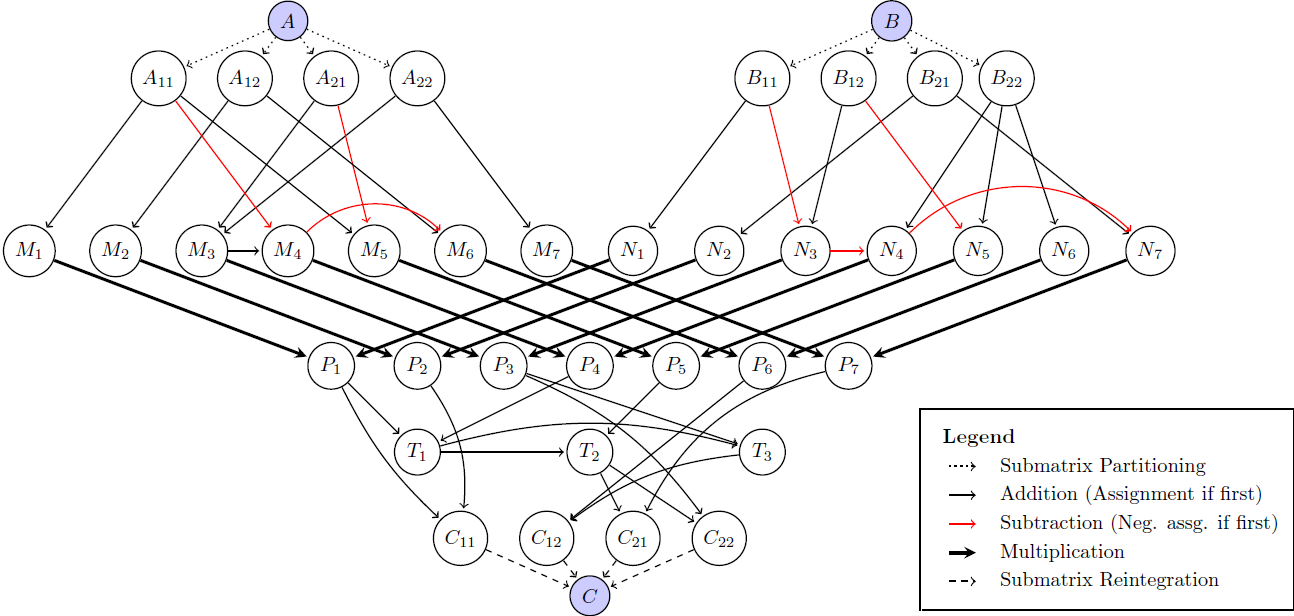
\includegraphics[width=0.85\textwidth]{Chapter2/images/StrassenAlgorithm} 
% \end{center}

% \center{\small{{\color{Grey}{\small\textit{Students aren't expected to be familiar with this material. It's presented to motivate matrix partitioning.}}}}}

% \end{frame}


% \begin{frame}\frametitle{The Fast Fourier Transform (FFT)}

% The FFT is an essential algorithm of modern technology that uses partitioned matrices recursively. 

% \begin{equation*}
% G_0 =  
% \begin{pmatrix}
% 1 
% \end{pmatrix}, \qquad  G _{n+1} = 
% \begin{pmatrix}
% G _n  & - G_n \\ G_n & G_n 
% \end{pmatrix}
% \end{equation*}

% \bigskip 

% \begin{columns}
% \begin{column}{.5\textwidth}
% \begin{center}
%  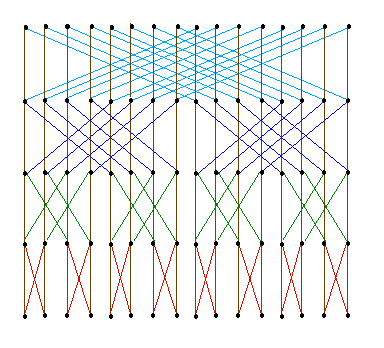
\includegraphics[width=0.8\textwidth]{Chapter2/images/fft1} 
% \end{center}
% \end{column}
% \begin{column}{.5\textwidth}
% \vskip .75cm
% The recursive structure of the matrix means that it can be computed in nearly \Emph{linear} time. This is an incredible saving over the general complexity of $ n ^{3}$.  It means that we can compute $ G_n x$, and $ G ^{-1}_n$ very quickly.  
% \end{column}
% \end{columns}


% \center{\small{{\color{Grey}{\small\textit{Students aren't expected to be familiar with this material. It is presented to motivate matrix partitioning.}}}}}

% \end{frame} 
    % \title{Partitioned Matrices and the Matrix Inverse}
\subtitle{\SubTitleName}
\institute[]{\Course}
\author{\Instructor}
\maketitle  







\frame{\frametitle{Topics and Objectives}
\Emph{Topics} \\
\TopicStatement
\begin{itemize}
    \item partitioned matrices (or block matrices)
    \item expressions for the inverse of a partitioned matrix
\end{itemize}

\vspace{0.5cm}

\Emph{Objectives}\\

\LearningObjectiveStatement

\begin{itemize}
    \item apply partitioned matrices to solve problems regarding matrix invertibility 
\end{itemize}

\vspace{0.25cm} 

%\Emph{Motivating Question} \\
%You have three group of variables $ X_1$, $ X_2, $ and $ X_3$. Within each group, they have many relationships, but between groups, only a few. What would the resulting matrix of relationships look like? 

}













\frame{\frametitle{The Row Column Method for Block Matrices}

    Partitioned matrices can be multiplied using this method, as if each block were a scalar (\textit{provided each block has appropriate dimensions so that products are defined}).
    
    \vspace{12pt}
    
    \pause
    
    How might we use this approach to determine an expression for the inverse of a matrix? 
}








\frame{\frametitle{Using the Row Column Method to Construct an Inverse}

    Recall, using our formula for a $2\times 2$ matrix,  $ \begin{pmatrix}
    a & b \\ 0 & c 
    \end{pmatrix} ^{-1} = \frac 1 {ac} \begin{pmatrix}
    c &  -b \\ 0 & a 
    \end{pmatrix}$.
    
    \pause 
    
    \vspace{0.5cm} 

    \Emph{Example}: Suppose $ A \in \R^{ n \times n}$, $B \in \R^{n\times n}$, and $C \in \R^{n\times n}$ are invertible matrices. Construct the inverse of $
    \begin{pmatrix}
        A & B \\ 0 & C 
    \end{pmatrix}
    $.

} 


\frame{\frametitle{Summary}

    \SummaryLine \vspace{4pt}
    \begin{itemize}\setlength{\itemsep}{8pt}
        \item using partitioned matrices to solve problems regarding matrix invertibility and matrix multiplication  
    \end{itemize}
    \vspace{4pt}
    Although not part of our course, matrix partitioning is often used to help derive new algorithms because they give a more concise representation of a matrix and of operations on matrices. 
}






% COLUMN ROW METHOD USUALLY NOT NEEDED IN THIS CLASS
% \frame{\frametitle{The Column Row Method (if time permits)}

% A column vector times a row vector is a matrix. For example,

% $$
% \begin{pmatrix}
% 1 \\ 0 \\ 2
% \end{pmatrix} 
% \begin{pmatrix}
% 1 & 3  
% \end{pmatrix} 
% = 
% %\begin{pmatrix} 1 & 3 \\ 0 & 0 \\ 2 & 6 \end{pmatrix}
% $$

% \begin{center}\begin{tikzpicture} \node [mybox](box){\begin{minipage}{0.8\textwidth}

% Let $ A$ be $ m \times n$ and $ B$ be $ n \times p$ matrix. Then,  
% \begin{align*}
%  AB &= 
%  \begin{pmatrix}
% \operatorname {col}_1 A & \cdots & \operatorname {col}_n A 
% \end{pmatrix}
%  \begin{pmatrix}
% \operatorname {row}_1 B \\ \vdots \\  \operatorname {row}_n B 
% \end{pmatrix}
% \\&= 
% \underbrace{
% \operatorname {col}_1 A \operatorname {row}_1 B + \cdots \operatorname {col}_n A \operatorname {row}_n B } 
% _{\textup{$ m \times p$ matrices}} 
% \end{align*}
% This is the \Emph{Column Row Method} for matrix multiplication.

% \end{minipage}};
% \node[fancytitle, right=10pt] at (box.north west) {Theorem};
% \end{tikzpicture}\end{center}


% }

% %% FRAME
% \begin{frame}\frametitle{The Strassen Algorithm: An impressive use of partitioned matrices}

% Naive Multiplication of two $ n \times n$ matrices $ A$ and $ B$ requires $ n ^3 $ arithmetic steps. 
% Strassen's algorithm \Emph{partitions} the matrices, makes a very clever sequence of multiplications, additions, to reduce the computation to $ n ^{2.803\ldots }$ steps.  


% \begin{center}
%     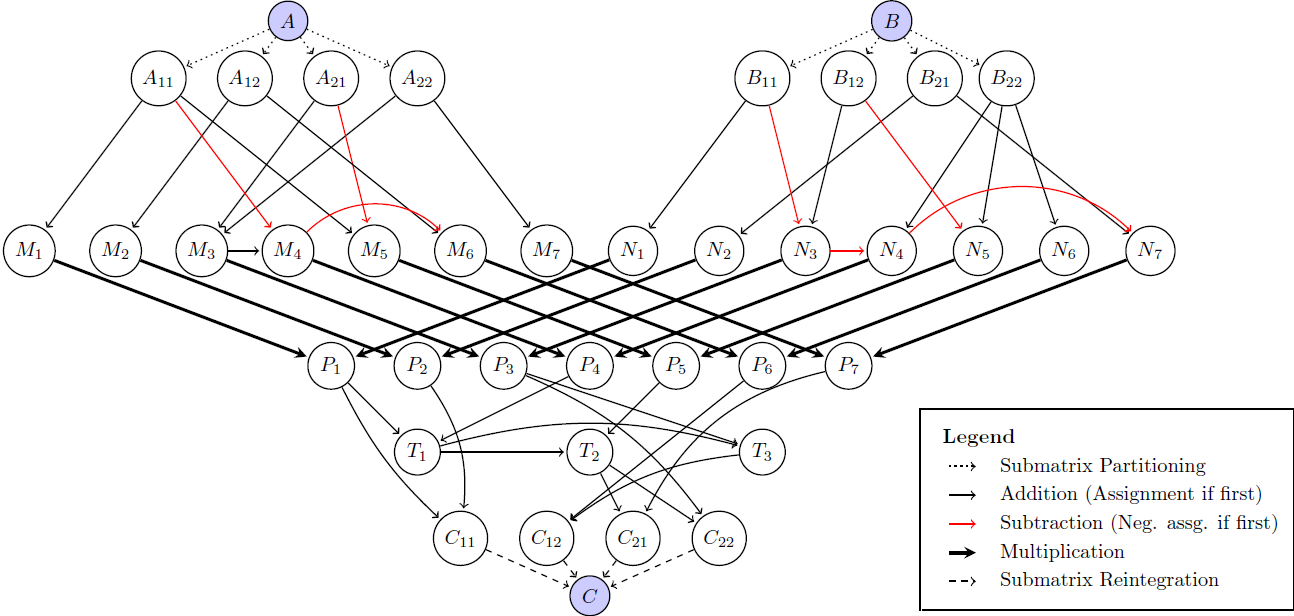
\includegraphics[width=0.85\textwidth]{Chapter2/images/StrassenAlgorithm} 
% \end{center}

% \center{\small{{\color{Grey}{\small\textit{Students aren't expected to be familiar with this material. It's presented to motivate matrix partitioning.}}}}}

% \end{frame}


% \begin{frame}\frametitle{The Fast Fourier Transform (FFT)}

% The FFT is an essential algorithm of modern technology that uses partitioned matrices recursively. 

% \begin{equation*}
% G_0 =  
% \begin{pmatrix}
% 1 
% \end{pmatrix}, \qquad  G _{n+1} = 
% \begin{pmatrix}
% G _n  & - G_n \\ G_n & G_n 
% \end{pmatrix}
% \end{equation*}

% \bigskip 

% \begin{columns}
% \begin{column}{.5\textwidth}
% \begin{center}
%  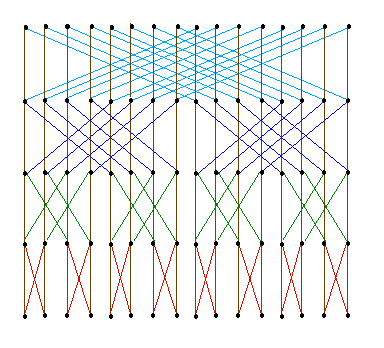
\includegraphics[width=0.8\textwidth]{Chapter2/images/fft1} 
% \end{center}
% \end{column}
% \begin{column}{.5\textwidth}
% \vskip .75cm
% The recursive structure of the matrix means that it can be computed in nearly \Emph{linear} time. This is an incredible saving over the general complexity of $ n ^{3}$.  It means that we can compute $ G_n x$, and $ G ^{-1}_n$ very quickly.  
% \end{column}
% \end{columns}


% \center{\small{{\color{Grey}{\small\textit{Students aren't expected to be familiar with this material. It is presented to motivate matrix partitioning.}}}}}

% \end{frame} 
    % \title{Solving Linear Systems with the LU Factorization}
\subtitle{\SubTitleName}
\institute[]{\Course}
\author{\Instructor}
\maketitle  








\frame{\frametitle{Topics and Objectives}
\Emph{Topics} \\
\TopicStatement
\begin{itemize}
    \item triangular matrices
    \item the LU factorization of a matrix 
    \item using the LU factorization to solve a system
\end{itemize}

\vspace{0.5cm}

\Emph{Objectives}\\

\LearningObjectiveStatement

\begin{itemize}
    \item identify and construct triangular matrices
    \item apply the LU factorization to solve systems of equations
\end{itemize}

\vspace{0.25cm} 

%\Emph{Motivating Question} \\

}

\frame{\frametitle{Mathematical Ingenuity}


    {\small \textit{``Mathematical reasoning may be regarded rather schematically as the exercise of a combination of two facilities, which we may call intuition and ingenuity." } \\- Alan Turing \\}
    
    \vspace{12pt}
    
    \pause 
    
    The use of the LU Decomposition to solve linear systems was one of the areas of mathematics that Turing helped develop. The decomposition is widely used to solve linear systems of equations. 

}





\frame{\frametitle{Motivation}

    \begin{itemize} 
        \item<1-> Recall that we \Emph{could} solve $A\vec x = \vec b$ by using $$\vec x = A^{-1} \vec b$$
    
        \item<2->  This requires computation of the inverse of an $n\times n$ matrix, which is especially difficult for large $n$. 
        
        \item<3-> Instead we could solve $A\vec x = \vec b$ with Gaussian Elimination, but this is not efficient for large $n$
    
        \item<4-> There are more efficient and accurate methods for solving linear systems that rely on matrix factorizations.
        
    \end{itemize}
}




\frame{\frametitle{Matrix Factorizations}

\begin{itemize}

    \item<1-> A \Emph{matrix factorization}, or \Emph{matrix decomposition} is a factorization of a matrix into a product of matrices.

    \item<2-> Factorizations can be useful for solving $A \vec x = \vec b$, or understanding the properties of a matrix.

    \item<3-> We explore a few matrix factorizations throughout this course.
    
    \item<4-> In this section, we factor a matrix into \Emph{lower} and into \Emph{upper} triangular matrices.
    
\end{itemize}


}



\frame{\frametitle{Triangular Matrices}

    Rectangular matrix $ A$ is \Emph{upper triangular} if $ a _{i,j} = 0$ for $ i > j$. Examples:
    
    $$
    \spalignmat{1 5 0;0 2 4}, \quad 
    \spalignmat{
    1 0 0 1;
    0 2 1 0;
    0 0 0 0;
    0 0 0 1}
    ,
    \quad
    \spalignmat{2 1;0 1;0 0;0 0}
    $$
 
    \pause 
    
    Rectangular matrix $ A$ is \Emph{lower triangular} if $ a _{i,j} = 0$ for $ i < j$. Examples:
    
    $$
    \spalignmat{1 0 0;3 2 0}, \quad 
    \spalignmat{
    3 0 0 0;
    1 1 0 0;
    0 0 0 0;
    0 2 0 1}
    ,
    \quad
    \spalignmat{1 0;1 4;0 1;2 0}
    $$
 

    \pause 
    
    Can you name a matrix that is both upper and lower triangular? 
}






\frame{\frametitle{The LU Factorization}

    \begin{center}\begin{tikzpicture} \node [mybox](box){\begin{minipage}{0.92\textwidth} 
        \vspace{2pt}

        If $ A$ is an $ m \times n$ matrix that can be row reduced to echelon form without row exchanges, then $ A = L U $. $ L $ is a lower triangular $ m \times m$ matrix with $ 1$'s on the diagonal, $ U$ is an \Emph{echelon} form of $ A$.

    \end{minipage}}; \node[fancytitle, right=10pt] at (box.north west) {Theorem}; \end{tikzpicture}\end{center}

    \pause 
    
    \Emph{Example}: If $A \in \mathbb R^{3\times 2}$, the LU factorization has the form:
        $$A = L U = \spalignmat{1 0 0 ;\ast, 1 0 ; \ast,\ast, 1 } \spalignmat{\ast , \ast; 0 , \ast; 0 0}$$


}

\frame{\frametitle{Using the LU Decomposition to Solve a Linear System}

    \Emph{Goal}: given rectangular matrix $A$ and vector $\vec b$, we wish to solve $A \vec x = \vec b$ for $\vec x$. \\ \vspace{12pt}
    
    \pause 
    
    \begin{center}\begin{tikzpicture} \node [mybox](box){\begin{minipage}{0.92\textwidth} 
        \vspace{2pt}

        To solve $A \vec x = \vec b$ for $\vec x$:

    \begin{enumerate}
        \item Construct the LU decomposition of $A$ to obtain $L$ and $U$. 
        \item Set $U\vec x = \vec y$. Forward solve for $ \vec y$ in $ L \vec y = \vec b$. 
        \item Backwards solve for $\vec x$ in $ U \vec x = \vec y$. 
    \end{enumerate}

    \end{minipage}}; \node[fancytitle, right=10pt] at (box.north west) {Algorithm}; \end{tikzpicture}\end{center}


    

}

\frame{\frametitle{Example of Solving a Linear System Given $A=LU$}

    \Emph{Example}: Solve the linear system $A\vec x = \vec b$, given the LU decomposition of $A$.
    \begin{equation*}
        A = LU = \spalignmat{1 0 0 0;1 1 0  0;0 2 1 0 ;0 0 1 1}\spalignmat{1 0 0;0 2 1;0 0 2; 0 0 0}, \quad \vec b = \spalignmat{2;3;2;0}
    \end{equation*}

}

\frame{\frametitle{Summary}

    \SummaryLine \vspace{4pt}
    \begin{itemize}\setlength{\itemsep}{8pt}
        \item triangular matrices
        \item using the LU factorization to solve linear systems
        % \item To compute the LU decomposition: 
        %     \begin{enumerate}
        %         \item Reduce $ A$ to an echelon form $ U$ by a sequence of row replacement operations, if possible.
        %         \item Place entries in $ L$ such that the same sequence of row operations reduces $ L$ to $ I$.
        % \end{enumerate}
        % \item The textbook offers a different explanation of how to construct the LU decomposition that students may find helpful. 
        % \item Another explanation on how to calculate the LU decomposition that students may find helpful is available from MIT OpenCourseWare: www.youtube.com/watch?v=rhNKncraJMk    
    \end{itemize}
    
    \vspace{18pt}
    To solve $A \vec x = LU \vec x = \vec b$, we follow this process:
    \begin{enumerate}
        \item construct the LU factorization
        \item forward solve for $ \vec y$ in $ L \vec y = \vec b$
        \item backwards solve for $\vec x$ in $ U \vec x = \vec y$
    \end{enumerate}

}



 
    % \title{Computing the LU Factorization}
\subtitle{\SubTitleName}
\institute[]{\Course}
\author{\Instructor}
\maketitle  








\frame{\frametitle{Topics and Objectives}
\Emph{Topics} \\
\TopicStatement
\begin{itemize}
    \item the LU factorization of a matrix 
    % \item Using the $LU$ factorization to solve a system
    \item why the LU factorization works
\end{itemize}

\vspace{0.5cm}

\Emph{Objectives}\\

\LearningObjectiveStatement

\begin{itemize}
    \item compute an LU factorization of a matrix
    % \item Apply the $LU$ factorization to solve systems of equations.
    % \item Determine whether a matrix has an $LU$ factorization.
\end{itemize}

\vspace{0.25cm} 

%\Emph{Motivating Question} \\

}






\frame{\frametitle{Why We Can Compute the LU Factorization}

Suppose $ A$ can be row reduced to echelon form $ U$ without interchanging rows.
\begin{equation*}
E_p \cdots E_1 A = U 
\end{equation*}
where the $ E _{j}$ are matrices that perform elementary row operations. Because we did not swap rows, each $E_j$ happens to be lower triangular and invertible. \pause Example:
\begin{equation*}
\begin{pmatrix*}[r]
1 & 0 & 0  \\ 0 & 1 & 0  \\ 2 & 0 & 1 
\end{pmatrix*} ^{-1} 
= \begin{pmatrix*}[r]
1 & 0 & 0  \\ 0 & 1 & 0  \\ -2 & 0 & 1 
\end{pmatrix*}
\end{equation*}
Therefore,  
\begin{equation*}
A = \underbrace{E_1 ^{-1} \cdots E _{p} ^{-1} } _{ = L } U = LU.
\end{equation*}
}






\frame{\frametitle{An Algorithm for Computing LU}

    To compute the LU decomposition: 

    \begin{enumerate}
        \item Reduce $ A$ to an echelon form $ U$ by a sequence of row replacement operations, if possible. 
        \item Place entries in $ L$ such that the same sequence of row operations reduces $ L$ to $ I$.
    \end{enumerate}

   

}





\frame{\frametitle{Example}

    Compute the $LU$ factorization of $A$. $$A = \spalignmat{4 -3 -1 5;-16 12 2 -17 ; 8 -6 -12 22 }$$
}



\frame{\frametitle{Final Notes on Computing LU}

    \begin{itemize}\setlength{\itemsep}{8pt}
    \item<1-> There are other definitions of the LU factorization that you may encounter in future courses or applications. 
    \item<2-> There are several other ways of computing this decomposition. 
    \item<3-> The only row operation we use to construct $L$ and $U$: \textit{replace a row with a multiple of a row above it}.
    \item<4-> As for the other two row operations: 
    \begin{itemize}\setlength{\itemsep}{4pt}
        \vspace{4pt}
        \item Multiplying a row by a non-zero scalar is not needed. 
    \item<5-> We cannot swap rows: more advanced linear algebra and numerical analysis courses address this limitation.  
    \end{itemize}
   \end{itemize}


}


\frame{\frametitle{Summary}

    \SummaryLine \vspace{4pt}
    \begin{itemize}\setlength{\itemsep}{8pt}
        \item why we can construct $A=LU$ when $A$ can be reduced to echelon form without row swaps
        \item constructing the LU decomposition using the following process
            \begin{enumerate}
                \item reduce $ A$ to an echelon form $ U$ by a sequence of row replacement operations, if possible
                \item place entries in $ L$ such that the same sequence of row operations reduces $ L$ to $ I$
        \end{enumerate}
    \end{itemize}
    
    \vspace{4pt}
    
    
        % \item Another explanation on how to calculate the LU decomposition that students may find helpful is available from MIT OpenCourseWare: www.youtube.com/watch?v=rhNKncraJMk    


}



    % \title{The Leontif Input-Output Model}
\subtitle{\SubTitleName}
\institute[]{\Course}
\author{\Instructor}
\maketitle  





\tikzstyle{E} =[rectangle, minimum width=1.5cm, minimum height=1.5cm, text centered, fill=DarkBlue!20]

\tikzstyle{W} = [rectangle, minimum width=1.5cm, minimum height=1.5cm, text centered, fill=DarkBlue!20]

\tikzstyle{ED} = [rectangle, minimum width=4cm, minimum height=2cm, text centered, fill=DarkBlue!20]

\tikzstyle{arrowred} = [very thick,->,>=stealth, dashed,DarkRed]
\tikzstyle{arrowblue} = [very thick,->,>=stealth, dashed,DarkBlue]


\frame{\frametitle{Topics and Objectives}
\Emph{Topics} \\
\TopicStatement
\begin{itemize}
\item the Leontief Input-Output model as a simple example of a model of an economy
\end{itemize}

\vspace{0.5cm}

\Emph{Objectives}\\

\LearningObjectiveStatement

\begin{itemize}
\item apply matrix algebra and inverses to construct and solve and analyze Leontif Input-Output problems
\end{itemize}

\vspace{0.25cm} 

% \Emph{Motivating Question} \\
% An economy consisting of 3 sectors: agriculture, manufacturing, and energy. The output of one sector is absorbed by all the sectors. If there is an increase in demand for energy, how does this impact the economy? 

}




\frame{\frametitle{Understanding the Underlying Concepts}

\textit{``Computers and robots replace humans in the exercise of mental functions in the same way as mechanical power replaced them in the performance of physical tasks." } \\ - Wassily Leontif, 1983 

\vspace{12pt}

\pause 

Students in linear algebra are, of course, required to demonstrate an understanding of underlying concepts behind procedures and algorithms. This is in part because computers are continuing to take on a much larger role in performing calculations. 



}





\frame{\frametitle{Example: An Economy with Two Sectors}

%\begin{columns}

%\begin{column}{.5\textwidth}

\begin{center}
\begin{tikzpicture}[node distance=2cm]
\node (E) [E] {E};
\node (W) [W, below of=E] {W};
\node (ED) [ED, right of=W, xshift=2cm, yshift=1cm] {external demands};
\draw [arrowred] (E) -- (ED);
\draw [arrowblue] (W) -- (ED);
\filldraw[DarkRed] (1.5,-0.36) circle (2pt);
\filldraw[DarkBlue] (1.5,-1.6) circle(2pt);
\draw[DarkRed, very thick, dashed,->, >=stealth] (1.5,-0.36) -- (0.3,-1.3);
\draw[DarkBlue, very thick, dashed,->, >=stealth] (1.5,-1.6) -- (0.3,-0.7);
\draw[DarkRed, very thick, dashed] (1.5,-0.36) -- (1.5,1);
\draw[DarkBlue, very thick, dashed] (1.5,-1.6) -- (1.5,-3);
\draw[DarkRed, very thick, dashed] (1.5,1) -- (0,1);
\draw[DarkBlue, very thick, dashed] (1.5,-3) -- (0,-3);
\draw[DarkRed, very thick, dashed,->, >=stealth] (0,1) -- (0,0.7);
\draw[DarkBlue, very thick, dashed,->, >=stealth] (0,-3) -- (0,-2.7);
\end{tikzpicture}
%\end{column}

%\begin{column}{.45\textwidth}
%%  ENUMERATE
\end{center} 

\begin{itemize}
    \item<1-> this economy contains two sectors: electricity (E), and water (W)
    \item<2-> the \textit{external demands} do not produce E and W
    \item<3-> how might we represent this economy with a set of linear equations?
\end{itemize}

}


\frame{\frametitle{The Leontif Model: Output Vector}
Suppose economy has $N$ sectors, with outputs measured by  $ \vec x \in \mathbb R^N$.  
\begin{align*} 
    \vec x & = \text{output vector} \\
    x_i &= \text{entry } i \text{ of vector } \vec x \\
    &= \text{number of units produced by sector } i
\end{align*}



}


\frame{\frametitle{The Leontif Model: Internal Consumption}

    The \Emph{consumption matrix}, $C$, describes how units are consumed by sectors to produce output. 
    
    \vspace{12pt}
    
    Two equivalent ways of defining entries of $C$.
    \begin{itemize}
        \item<2-> sector $i$ \Emph{sends} a proportion of its units to sector $j$, call it $ c _{i,j}x_i$
        \item<3-> sector $j$ \Emph{requires} a proportion of the units created by sector $i$, call it $ c _{i,j}x_i$
    \end{itemize}
    
    \vspace{12pt}
    
    \onslide<4->{
    Entries of $C$ are $c _{i,j}$, with $c _{i,j} \in[0,1]$, and 
    } 
    \onslide<5->{
    \begin{align*} 
        C\vec x &= \text{units consumed} \\
        \vec x - C\vec x &= \text{units left after internal consumption}
    \end{align*}
    }

}





\frame{\frametitle{Example With Three Sectors}

    An economy contains three sectors, E, W, M. 
    
    \vfill 
    
    For every 100 units of output, 
    \begin{itemize} 
    \item E requires 20 units from E, 10 units from W, and 10 units from M
    \item W requires 0 units from E, 20 units from W, and 10 units from M
    \item M requires 0 units from E, 0 units from W, and 20 units from M
    \end{itemize}
    
    \vfill 
    
    \pause 
    
    If the output vector is $\vec x = \spalignmat{x_E;x_W;x_M}$, construct the consumption matrix for this economy. 

}





\frame{\frametitle{Sketching a Graph for the Economy}
    
    Although not strictly necessary, it can help to sketch the graph for the economy. 
    \begin{center}
    \begin{tikzpicture}
    \begin{scope}[->,>=stealth',shorten >=1pt,auto,node distance=2.2cm,
      thick,main node/.style={circle,fill=DarkBlue!20,draw,font=\sffamily\Large\bfseries}]
        \node[main node] (1) {E};
        \node[main node] (2) [right of=1] {W};
        \node[main node] (3) [below of=2] {M};
        \path[every node/.style={font=\sffamily\small}]
        (1) edge [loop left] node {20\%} (1)
        (2) edge node [above] {10\%} (1)
            edge [loop right] node {20\%} (2)
        (3) edge [bend left] node [above right] {10\%} (1)
            edge node [right] {10\%} (2)
            edge [loop right] node {20\%} (3);
    \end{scope}
    \end{tikzpicture}  
    \end{center}
}
    
  


\frame{\frametitle{Solution: Creating $C$}

    Our consumption matrix is
    $$C = \frac{1}{10} \spalignmat{2 0 0;1 2 0; 1 1 2} $$
    Note: 
    \begin{itemize}
        \item total output for each sector is the sum along the outgoing edges for each sector, which generates rows of $C$
        \item elements of $C$ represent percentages with no units, they have values between 0 and 1
        \item our output vector has units
    \end{itemize}

}

\frame{\frametitle{The Leontif Model: Demand}

\vspace{6pt}

There is also an external demand given by $ \vec d \in \mathbb R^N$. We ask if there is an $\vec x$ such that
$$\vec x -  C \vec x = \vec d$$
We can re-write this as 
$$ (I - C)\vec x = \vec d$$
This matrix equation is the \Emph{Leontief Input-Output Model}. Solving for $\vec x$ gives the output that meets external demand exactly.


}  

\frame{\frametitle{Example Revisited}

    Now suppose there is an external demand: what production level is required to satisfy a final demand of 80 units of E, 70 units of W, and 160 units of M?
    
    \vspace{4pt}
    \begin{center}
\begin{tikzpicture}
\begin{scope}[->,>=stealth',shorten >=1pt,auto,node distance=3.4cm,
  thick,main node/.style={circle,fill=DarkBlue!20,draw,font=\sffamily\Large\bfseries}]
  \node[main node] (1) {E};
  \node[main node] (2) [right of=1] {W};
    \node[main node] (3) [below of=2] {M};
    \node[main node] (4) [below of=1] {D};
  \path[every node/.style={font=\sffamily\small}]
    (1) edge [loop left] node {20\%} (1)
        edge [DarkRed] node[left] {80 units} (4)
    (2) edge node [above] {10\%} (1)
        edge [loop right] node {20\%} (2)
        edge [bend right, DarkRed] node[above left] {} (4)
    (3) edge [bend left] node [above right] {10\%} (1)
        edge node [right] {10\%} (2)
        edge [loop right] node {20\%} (3)
        edge [DarkRed] node[below] {160 units}  (4);
\end{scope}
        \draw (2,-1.2) node [DarkRed] {70 units};
        \end{tikzpicture}  
            \end{center}
}
    

\frame{\frametitle{Solution}
The production level would be found by solving:
    \begin{align*}
    (I - C)\vec x &= \vec d \\
        \frac{1}{10} \spalignmat{8 0 0;-1 8 0; -1 -1 8} \vec x &= \spalignmat{80;70;160} \\
        8x_1 &= 800 \quad \Rightarrow \quad x_1 = 100\\
        -x_1 + 8x_2 &= 700 \quad \Rightarrow \quad x_2 = 100 \\
        -x_1 - x_2 + 8x_3 &= 1600 \quad
        \Rightarrow \quad x_3 = 1800/8 = 225
    \end{align*}
    \pause
    The output that balances demand with internal consumption is $\vec x = \spalignmat{100;100;225 }.$
}



% \frame{\frametitle{The Importance of $(I-C)^{-1}$}

% For the example above
% \begin{equation*}
% (I-C) ^{-1} \approx \spalignmat{1.25,0,0;0.15,1.25,0;0.18,0.17,1.25}
% \end{equation*}


% The entries of $ (I - C) ^{-1} = B$ have this meaning:  if the final demand vector $ \vec d$ increases by one unit in the $ j^{th}$ place, the column vector $ b_j$ is the additional output required from other sectors.  


% \bigskip 
% So to meet an increase in demand for M by one unit, requires 1.25 of one additional units from M to meet internal consumption.  

% }







\frame{\frametitle{Summary}

    \SummaryLine \vspace{4pt}
    \begin{itemize}\setlength{\itemsep}{8pt}
        \item setting up and solving Leontif input-output models
    \end{itemize}
    
    \vspace{4pt}
    
    This video explored an application of systems of equations.
    



}



\frame{
}
 
 \fi 

% \ifnum \Week = 6
%     \newcommand{\SubTitleName}{Matrix Algebra}
    % \title{Homogeneous Coordinates}
\subtitle{\SubTitleName}
\institute[]{\Course}
\author{\Instructor}
\maketitle  



% \tikzstyle{E} =[rectangle, minimum width=1.5cm, minimum height=1.5cm, text centered, fill=DarkBlue!30]

% \tikzstyle{W} = [rectangle, minimum width=1.5cm, minimum height=1.5cm, text centered, fill=DarkBlue!30]

% \tikzstyle{ED} = [rectangle, minimum width=2cm, minimum height=3cm, text centered, fill=DarkBlue!30]

% \tikzstyle{arrowred} = [thick,->,>=stealth, dashed,DarkRed]
% \tikzstyle{arrowblue} = [thick,->,>=stealth, dashed,DarkBlue]


\frame{\frametitle{Topics and Objectives}
\Emph{Topics} \\
\TopicStatement
\begin{itemize}
    \item homogeneous coordinates in 2D
    \item translations and composite transforms in 2D
\end{itemize}

\vspace{0.5cm}

\Emph{Objectives}\\

\LearningObjectiveStatement

\begin{itemize}
    \item construct a data matrix to represent points in $\mathbb R^2$ using homogeneous coordinates
    \item construct and apply transformation matrices to represent composite transforms in 2D using homogeneous coordinates
\end{itemize}

% Students are not expected to be familiar with perspective projections.

\vspace{0.25cm} 
 

}





\frame{\frametitle{Motivating Questions} 

    How can we represent translations, and rotations about arbitrary points, using linear transforms? 
    \begin{itemize}\setlength{\itemsep}{4pt}
        \item transformations of the form $T(\vec x) = A\vec x$ were explored earlier in this course
        \item we introduced rotations about the origin, but not about arbitrary points
        \item we also did not explore the transform $(x,y) \to (x+h,y+k)$
    \end{itemize}}





\frame{\frametitle{Homogeneous Coordinates}

    Translations of points in $\mathbb R^n$ does not correspond directly to a linear transform. \Emph{Homogeneous coordinates} are used to model translations using matrix multiplication.  
    
    \begin{center}\begin{tikzpicture} \node [mybox](box){\begin{minipage}{0.95\textwidth} \vspace{2pt}
    Each point $(x,y)$ in $\mathbb R^2$ can be identified with the point $(x,y,H)$, $H\ne 0$, on the plane in $\mathbb R^3$ that lies $H$ units above the $xy$-plane. 
     \end{minipage}}; \node[fancytitle, right=10pt] at (box.north west) {Homogeneous Coordinates in $\mathbb R^2$}; \end{tikzpicture}\end{center}
     
    Note: we often we set $H = 1$. \\[6pt]

}





\frame{\frametitle{Homogeneous Coordinates Example}

    A translation of the form $(x,y) \to (x+h,y+k)$ can be represented as a matrix multiplication with homogeneous coordinates: 
    
    $$\spalignmat{1 0 h;0 1 k;0 0 1} \spalignmat{x;y;1} = \spalignmat{x+h;y+k;1}$$

}









\frame{\frametitle{A Composite Transform with Homogeneous Coordinates}

    Triangle $S$ is determined by three data points, $(1,1), (2,4), (3,1)$. \\[6pt]
    
    Transform $T$ rotates points by $\pi/2$ radians counterclockwise about the point $(0,1)$.
    
    \vspace{6pt}
    
    \begin{enumerate}[a)]
        \item Represent the data with a matrix, $D$. Use homogeneous coordinates. 
        \item Use matrix multiplication to determine the image of $S$ under $T$. 
        \item Sketch $S$ and its image under $T$. 
    \end{enumerate}

}



\frame{\frametitle{Summary}

    \SummaryLine \vspace{4pt}
    \begin{itemize}\setlength{\itemsep}{8pt}
        \item homogeneous coordinates
        \item constructing composite transforms that apply translations and rotations about arbitrary points in $\mathbb R^2$
    \end{itemize}
    
}
 
    % \title{3D Transformations}
\subtitle{\SubTitleName}
\institute[]{\Course}
\author{\Instructor}
\maketitle  



\tikzstyle{E} =[rectangle, minimum width=1.5cm, minimum height=1.5cm, text centered, fill=DarkBlue!30]

\tikzstyle{W} = [rectangle, minimum width=1.5cm, minimum height=1.5cm, text centered, fill=DarkBlue!30]

\tikzstyle{ED} = [rectangle, minimum width=2cm, minimum height=3cm, text centered, fill=DarkBlue!30]

\tikzstyle{arrowred} = [thick,->,>=stealth, dashed,DarkRed]
\tikzstyle{arrowblue} = [thick,->,>=stealth, dashed,DarkBlue]


\frame{\frametitle{Topics and Objectives}
    \Emph{Topics} \\
    \TopicStatement
    \begin{itemize}
    \item homogeneous coordinates in 3D
    \item translations and composite transforms in 3D
    \end{itemize}
    
    \vspace{0.5cm}
    
    \Emph{Objectives}\\
    
    \LearningObjectiveStatement
    
    \begin{itemize}
    \item construct a data matrix to represent points in $\mathbb R^3$ with homogeneous coordinates
    \item construct and apply transformation matrices to represent composite transforms in 3D using homogeneous coordinates
    \end{itemize}
    
    % In the interest of time, students are not expected to be familiar with perspective projections.

}







\frame{\frametitle{3D Homogeneous Coordinates}

    Homogeneous coordinates in 3D are analogous to our 2D coordinates. 
    
    \begin{center}\begin{tikzpicture} \node [mybox](box){\begin{minipage}{0.75\textwidth} \vspace{4pt}
        $(X,Y,Z,1)$ are homogeneous coordinates for $(x,y,z)$ in $\mathbb R^3$ %, and $$x = \frac X H, \quad y = \frac Y H, \quad z = \frac Z H$$
     \end{minipage}}; \node[fancytitle, right=10pt] at (box.north west) {Homogeneous Coordinates in $\mathbb R^3$}; \end{tikzpicture}\end{center}
 
    \vspace{6pt}
    
    % For example, $(a,b,c,1)$ and $(3a,3b,3c,3)$ are both homogeneous coordinates for the point $(a,b,c)$. 

}

\frame{\frametitle{Homogeneous Coordinates Example}

    A translation of the form $(x,y,z) \to (x+h,y+k,z+l)$ can be represented as a matrix multiplication with homogeneous coordinates: 
    
    $$\spalignmat{1 0 0 h;0 1 0 k;0 0 1 l; 0 0 0 1} \spalignmat{x;y;z;1} = \spalignmat{x+h;y+k;z+l;1}$$

}



\frame{\frametitle{3D Transformation Matrices}

    Construct matrices for the following transformations. 
    
    \begin{enumerate}[a)]
        \item A translation in $\mathbb R^3$ specified by the vector $\vec p = \spalignmat{-2;3;4}$.
        \item A rotation in $\mathbb R^3$ about the $x_2$-axis by $\pi$ radians. 
        \item A projection onto the plane $x_3=4$. 
    \end{enumerate}    
    \vspace{12pt}
    \textit{For any of the above, it is ok to leave your answer as a product of matrices. }
}



\frame{\frametitle{Summary}

    \SummaryLine \vspace{4pt}
    \begin{itemize}\setlength{\itemsep}{8pt}
        \item constructing composite transforms that apply translations and rotations about arbitrary points in $\mathbb R^3$
    \end{itemize}
    

}
 
    % \title{Subsets and Subspaces}
\subtitle{\SubTitleName}
\institute[]{\Course}
\author{\Instructor}
\maketitle  



\frame{\frametitle{Topics and Objectives}
\Emph{Topics} \\
\TopicStatement
\begin{itemize}
    \item subsets and subspaces
    \item set builder notation
\end{itemize}

\vspace{0.5cm}

\Emph{Objectives}\\

\LearningObjectiveStatement

\begin{itemize}
    \item determine whether a subset of $\mathbb R^n$ is a subspace
    % \item determine whether a vector is in a particular subspace, or find a vector in that subspace
    % \item construct a basis for a subspace (for example, a basis for Col(A))
\end{itemize}


}


\frame{\frametitle{Subsets of $\mathbb R^n$}

    
    \begin{center}\begin{tikzpicture} \node [mybox](box){\begin{minipage}{0.80\textwidth}\vspace{2pt}

        A \Emph{subset of $\mathbb R^n$} is any collection of vectors that are in $\mathbb R^n$.
        
    \end{minipage}};\node[fancytitle, right=10pt] at (box.north west) {Definition};
    \end{tikzpicture}\end{center}
    
    \Emph{Examples}
    \begin{itemize}
        \item the span of the columns of a $3\times4$ matrix is a subset of $\mathbb R^3$
        \item the set of all vectors of the form $\spalignmat{1;k}$ is a subset of  $\mathbb R^2$
    \end{itemize}
    
}

\frame{\frametitle{Subspaces in $\mathbb R^n$}

    % ~~ ~~ Highlight Box ~~ ~~
    \begin{center}\begin{tikzpicture} \node [mybox](box){\begin{minipage}{0.90\textwidth}\vspace{2pt}

    A subset $ H $ of $ \mathbb R ^{n}$ is a \Emph{subspace} if it is closed under scalar multiplies and vector addition.  That is: for any $c\in\mathbb R$ and for $\vec u,  \vec v\in H$, 

    \begin{enumerate}
        \item $c \,\vec u  \in H$
        \item $\vec u + \vec v \in H$
    \end{enumerate}
    \end{minipage}};\node[fancytitle, right=10pt] at (box.north west) {Definition};
    \end{tikzpicture}\end{center}

    Note that condition 1 implies that the zero vector must be in $H$.

}



\frame{\frametitle{Example: Subspaces}
    Which of the following subsets could be a subspace of $\R^2$? 

    \begin{center}
    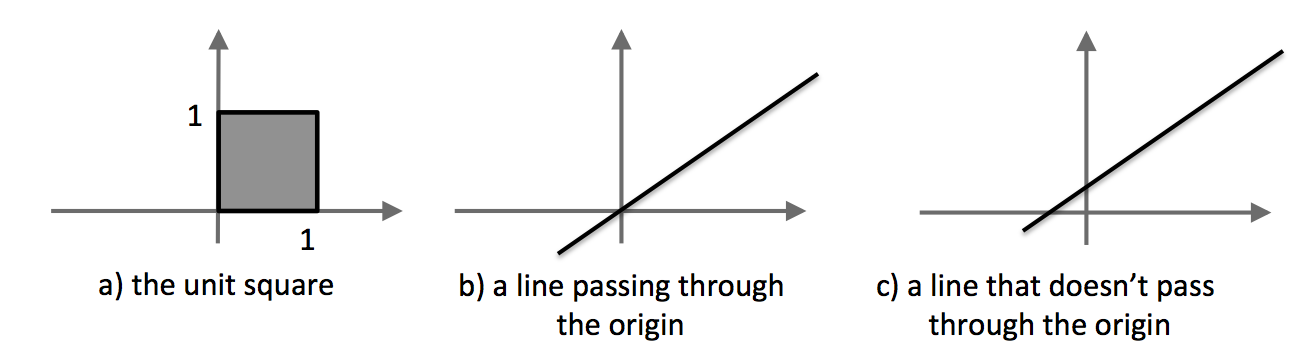
\includegraphics[width=0.95\textwidth]{Chapter2/images/subspaces.png} 
    \end{center}

}

\frame{\frametitle{Example: Set Builder Notation}

    Let $V = \left\{ \spalignmat{a ; b} \in \mathbb R^2 \ | \ ab = 0 \right\}$. 
    \begin{enumerate} 
        \item Give an example of at least two vectors that are in $V$. 
        \item Give an example of at least two vectors that are not in $V$. 
        \item Is the zero vector in $V$? 
        \item Is $V$ a subspace? 
    \end{enumerate}

}




\frame{\frametitle{Summary}

    \SummaryLine \vspace{4pt}
    \begin{itemize}\setlength{\itemsep}{8pt}
        \item identifying whether a subset is a subspace
    \end{itemize}
    

} 
    % 
\title{Column Space and Null Space}
\subtitle{\SubTitleName}
\institute[]{\Course}
\author{\Instructor}
\maketitle  



\frame{\frametitle{Topics and Objectives}
\Emph{Topics} \\
\TopicStatement
\begin{itemize}
    \item the column space and null space of a matrix
\end{itemize}

\vspace{0.5cm}

\Emph{Objectives}\\

\LearningObjectiveStatement

\begin{itemize}
    \item determine whether a vector is a column or null space of a matrix, or identify a vector in that subspace
    \item construct a matrix whose column and/or null space is given
    % \item construct a basis for a subspace (for example, a basis for Col(A))
\end{itemize}


}


\frame{\frametitle{The Column Space and the Null Space of a Matrix}

    \Emph{Recall}: for $ \vec v_1 ,\dotsc, \vec v_p \in \mathbb R ^{n}$, that
$ \operatorname {Span} \{\vec v_1 ,\dotsc, \vec v_p\}$ is: the set of all possible linear combinations of the vectors $ \vec v_j$. 

    \vspace{12pt} 
    
    
    This is a \Emph{subspace}, spanned by $ \vec v_1 ,\dotsc, \vec v_p$.  

    \pause 

    % ~~ ~~ Highlight Box ~~ ~~
    \begin{center}\begin{tikzpicture} \node [mybox](box){\begin{minipage}{0.90\textwidth}\vspace{2pt}

    Given an $ m \times n $ matrix $ A = \begin{bmatrix}
    \vec a_1 & \cdots & \vec a _{n}
    \end{bmatrix}$ \vspace{2pt}
    \begin{itemize}
        \item  The \Emph{column space of $ A$}, $ \operatorname {Col} A $, is the subspace of $ \mathbb R ^{m}$ spanned by $ \vec a_1 ,\dotsc, \vec a_n$.  \vspace{2pt}
        \item The \Emph{null space of $A$}, $ \operatorname {Null} A $, is the subspace of $\mathbb R^n$ spanned by the set of all vectors $ \vec x$ that solve $ A \vec x= \vec 0$. 
    \end{itemize}
    \end{minipage}};\node[fancytitle, right=10pt] at (box.north west) {Definition};
    \end{tikzpicture}\end{center}

}






\frame{\frametitle{Example: Column Space}
Is $\vec b$ in the column space of $A$? 
$$A = \spalignmat{1 -3 -4;-4 6 -2;-3 7 6} 
% \sim \spalignmat{1 -3 -4 ;0 -6 -18; 0 0 0}
, \quad \vec b = \spalignmat{ 3 ; 3; -4}
$$
}

\frame{\frametitle{Example: Null Space}
Using the matrix on the previous slide: is $\vec v$ in the null space of $A$?  $$A = \spalignmat{1 -3 -4;-4 6 -2;-3 7 6} , \quad \vec v = \spalignmat{-5\lambda ; -3\lambda; \lambda }, \quad \lambda \in \mathbb R $$
}
 
 
 
\frame{\frametitle{Example: Column and Null Space}
Give an example of a vector in the column space of $A$, and a vector in the null space of $A$. $$A = \spalignmat{1 0 0 4;0 1 3 0;0 0 0 0}$$ 
}

\frame{\frametitle{Example Construction}
Give an example of a matrix whose column space is spanned by $\spalignmat{1;1}$ and whose null space is spanned by $\spalignmat{2;1}$. 
}
 
 



\frame{\frametitle{Summary}

    \SummaryLine \vspace{4pt}
    \begin{itemize}\setlength{\itemsep}{8pt}
        \item determining whether a vector is a column or null space of a matrix
        \item identifying vectors in the column and null space of a matrix
        \item constructing a matrix whose column and/or null space is given   
    \end{itemize}
    

}     
    % \title{The Basis of a Subspace}
\subtitle{\SubTitleName}
\institute[]{\Course}
\author{\Instructor}
\maketitle  



\frame{\frametitle{Topics and Objectives}
\Emph{Topics} \\
\TopicStatement
\begin{itemize}
    % \item subspaces, Column space, and Null spaces 
    \item a basis for a subspace
\end{itemize}

\vspace{0.5cm}

\Emph{Objectives}\\

\LearningObjectiveStatement

\begin{itemize}
    % \item determine whether a set is a subspace
    % \item determine whether a vector is in a particular subspace, or find a vector in that subspace
    \item construct a basis for a subspace (for example, a basis for Col(A))
\end{itemize}

}


 
\frame{\frametitle{Basis}

    % ~~ ~~ Highlight Box ~~ ~~
    \begin{center}\begin{tikzpicture} \node [mybox](box){\begin{minipage}{0.80\textwidth}\vspace{2pt}

    A \Emph{basis} for a subspace $ H$ is a set of linearly independent vectors in $H$ that span $ H$. 

    \end{minipage}};\node[fancytitle, right=10pt] at (box.north west) {Definition};
    \end{tikzpicture}\end{center}
    
    \pause

    \Emph{Example} \\
    The set $ H = \{  \vec x \in \mathbb R^4 \; \large| \; x_1 - 3x_2 - 5x_3 + 7x_4=0\}$ is a subspace. 
    \begin{enumerate}[a)]
        \item $H$ is a null space for what matrix $A$?
        \item Construct a basis for $H$. 
    \end{enumerate}


}

\frame{\frametitle{Example}

    Construct a basis for Null$A$ and a basis for Col$A$.
    \begin{equation*} A=
    \begin{pmatrix*}[r]
    -3 & 6 & -1  & 0 
    \\
    1 & -2 & 2  & 0 
    \\
    2 & -4 & 5  & 0 
    \end{pmatrix*}
    \sim 
    \begin{pmatrix*}[r]
    1 & -2 & 0  & 0 
    \\
    0 & 0& 1  & 0 
    \\
    0 & 0 & 0  & 0 
    \end{pmatrix*}
    \end{equation*}
}



\frame{\frametitle{Summary}

    \SummaryLine \vspace{4pt}
    \begin{itemize}\setlength{\itemsep}{8pt}
        \item constructing a basis for a subspace
        \item constructing a basis for the column and/or null space of a matrix
    \end{itemize}
    

}         
    % \title{Coordinate Systems}
\subtitle{\SubTitleName}
\institute[]{\Course}
\author{\Instructor}
\maketitle  


\frame{\frametitle{Topics and Objectives}
\Emph{Topics} \\
\TopicStatement
\begin{itemize}
    \item change of basis
    \item coordinates relative to a basis
    % \item dimension of a subspace
    % \item the rank of a matrix 
\end{itemize}

\vspace{0.5cm}

\Emph{Objectives}\\

\LearningObjectiveStatement

\begin{itemize}
    \item calculate the coordinates of a vector in a given basis
    % \item characterize a subspace using the concept of dimension (or cardinality)
    % \item characterize a matrix using the concepts of rank, column space, null space
    % \item apply the rank, basis, and matrix invertibility theorems to describe matrices and subspaces
\end{itemize}
 
}

\frame{\frametitle{Choice of Basis}

\Emph{Key idea:} There are many possible choices of basis for a subspace. Our choice can give us dramatically different properties.

\vspace{0.5cm}

\pause 

\Emph{Example}: sketch $\vec b_1 + \vec b_2$ for the two different coordinate systems below. 

\begin{center}
  \begin{tikzpicture}

    \usetikzlibrary{calc}
    \begin{scope}[xshift=6cm, scale=1.1] 
    
    \coordinate (Origin)   at (0,0);
    \coordinate (XAxisMin) at (-1,0);
    \coordinate (XAxisMax) at (3,0);
    \coordinate (YAxisMin) at (0,-1);
    \coordinate (YAxisMax) at (0,3);
    \draw [thin, gray,-latex] (XAxisMin) -- (XAxisMax);% Draw x axis
    \draw [thin, gray,-latex] (YAxisMin) -- (YAxisMax);% Draw y axis

   \clip (-1,-1) rectangle (3,3); % Clips the picture...
%    \pgftransformcm{1}{0.6}{0.7}{1}{\pgfpoint{0cm}{0cm}}
          % This is actually the transformation matrix entries that
          % gives the slanted unit vectors. You might check it on
           % MATLAB etc. . I got it by guessing.
    \coordinate (Bone) at (0,1);
    \coordinate (Btwo) at (1,-1);
    \draw[style=help lines,dashed] (-14,-14) grid[step=1cm] (14,14);
          % Draws a grid in the new coordinates.
          %\filldraw[fill=gray, fill opacity=0.3, draw=black] (0,0) rectangle (2,2);
              % Puts the shaded rectangle
    \foreach \x in {-7,-6,...,7}{% Two indices running over each
      \foreach \y in {-7,-6,...,7}{% node on the grid we have drawn 
        \node[draw,circle,inner sep=1pt,fill] at (\x,\y) {};
            % Places a dot at those points
      }
    }
    \draw [ultra thick,-latex,DarkRed] (Origin) -- (Bone) node [above left] {$\vec b_2$};
%    \draw [ultra thick,-latex,red] (Origin) -- (Btwo) node [below right] {$2b_2$};
   \draw [ultra thick,-latex,DarkRed] (Origin) -- ($(Bone)+(Btwo)$) node [below right] {$\vec b_1$};
    %\draw [ultra thick,-latex,red] (Origin) -- ($2*(Bone)+(Btwo)$) node [above right] {$2\vec b_1+2\vec b_2$};
%    \filldraw[fill=gray, fill opacity=0.3, draw=black] (Origin) rectangle ($2*(Bone)+(Btwo)$);
    %\draw [thin,-latex,red, fill=gray, fill opacity=0.3] (0,0)
        % -- ($2*(0,2)+(2,-2)$)
        % -- ($3*(0,2)+2*(2,-2)$) -- ($(0,2)+(2,-2)$) -- cycle;
    \end{scope}

    \begin{scope}[scale=.75]
    
    \coordinate (Origin)   at (0,0);
    \coordinate (XAxisMin) at (-1,0);
    \coordinate (XAxisMax) at (4,0);
    \coordinate (YAxisMin) at (0,-1);
    \coordinate (YAxisMax) at (0,4);
    \draw [thin, gray,-latex] (XAxisMin) -- (XAxisMax);% Draw x axis
    \draw [thin, gray,-latex] (YAxisMin) -- (YAxisMax);% Draw y axis

   \clip (-1,-1) rectangle (4,4); % Clips the picture...
    \pgftransformcm{1}{0.6}{0.7}{1}{\pgfpoint{0cm}{0cm}}
          % This is actually the transformation matrix entries that
          % gives the slanted unit vectors. You might check it on
           % MATLAB etc. . I got it by guessing.
    \coordinate (Bone) at (0,2);
    \coordinate (Btwo) at (2,-2);
    \draw[style=help lines,dashed] (-14,-14) grid[step=2cm] (14,14);
          % Draws a grid in the new coordinates.
          %\filldraw[fill=gray, fill opacity=0.3, draw=black] (0,0) rectangle (2,2);
              % Puts the shaded rectangle
    \foreach \x in {-7,-6,...,7}{% Two indices running over each
      \foreach \y in {-7,-6,...,7}{% node on the grid we have drawn 
        \node[draw,circle,inner sep=1pt,fill] at (2*\x,2*\y) {};
            % Places a dot at those points
      }
    }
    \draw [ultra thick,-latex,DarkRed] (Origin)
        -- (Bone) node [above ] {$\vec b_2$};
    %\draw [ultra thick,-latex,red] (Origin) -- (Btwo) node [below right] {$b_2$};
    \draw [ultra thick,-latex,DarkRed] (Origin) -- ($(Bone)+(Btwo)$) node [ right] {$\vec b_1$};
    %\draw [ultra thick,-latex,red] (Origin) -- ($2*(Bone)+(Btwo)$) node [above left] {$\vec b_1+ \vec b_2$};
    %\filldraw[fill=gray, fill opacity=0.3, draw=black] (Origin) rectangle ($2*(Bone)+(Btwo)$);
    %\draw [thin,-latex,red, fill=gray, fill opacity=0.3] (0,0)
        % -- ($2*(0,2)+(2,-2)$)
        % -- ($3*(0,2)+2*(2,-2)$) -- ($(0,2)+(2,-2)$) -- cycle;
    \end{scope}
        
  \end{tikzpicture}

\end{center}
}

\frame{\frametitle{Definition: Coordinate Vector}

    Let $ \mathcal B = \{\vec b_1 ,\dotsc, \vec b_p\}$ be a basis for a subspace $ H$.  
    If $\vec x$ is in $H$, then \Emph{coordinates of $ \vec x$ relative $ \mathcal B$} are the weights (scalars) $ c_1 ,\dotsc, c_p$ so that 
    $$ \vec x = c_1 \vec b_1 + \cdots + c_p \vec b _p $$
    
    \pause 
    
    And 
    \begin{equation*}
    [x] _{\mathcal B} = 
    \begin{bmatrix*}[r]
    c_1 \\ \vdots \\ c_p 
    \end{bmatrix*}
    \end{equation*}
    is the \Emph{coordinate vector of $ \vec x$ relative to $ \mathcal B$}, or the \Emph{$ \mathcal B$-coordinate vector of $ \vec x$}

}

\frame{\frametitle{Example: Coordinate Vector}
    Let $ \vec v_1 = \begin{bmatrix*}[r]
    1 \\ 0 \\ 1
    \end{bmatrix*}$, 
    $ \vec v_2 = \begin{bmatrix*}[r] 1 \\ 1 \\ 1  \end{bmatrix*}$, 
    and 
    $ \vec x =\begin{bmatrix*}[r]
    5 \\ 3 \\ 5
    \end{bmatrix*}$.  Verify that $\vec  x $ is in the span of $ \mathcal B= \{\vec v_1 , \vec v_2\}$, and calculate  
    $ [\vec x] _{\mathcal B}$. 

}


\frame{\frametitle{Summary}

    \SummaryLine \vspace{4pt}
    \begin{itemize}\setlength{\itemsep}{8pt}
        \item calculating the coordinates of a vector with a given basis for a subspace
    \end{itemize}
    

} 
    % \title{The Dimension of a Susbpsace}
\subtitle{\SubTitleName}
\institute[]{\Course}
\author{\Instructor}
\maketitle  


\frame{\frametitle{Topics and Objectives}
\Emph{Topics} \\
\TopicStatement
\begin{itemize}
    \item dimension of a subspace
    % \item the rank of a matrix 
\end{itemize}

\vspace{0.5cm}

\Emph{Objectives}\\

\LearningObjectiveStatement

\begin{itemize}
    \item characterize a subspace using the concept of dimension (or cardinality)
    % \item characterize a matrix using the concepts of rank, column space, null space
    % \item apply the rank, basis, and matrix invertibility theorems to describe matrices and subspaces
\end{itemize}
 
}





\frame{\frametitle{Dimension of a Subspace}

    \vspace{-12pt}
    \begin{center}\begin{tikzpicture} \node [mybox](box){\begin{minipage}{0.85\textwidth} \vspace{2pt}
    
    The \Emph{dimension} (or cardinality) of a non-zero subspace $H$, $ \operatorname {dim} H $, is the number of vectors in a basis of $H$.
    We define $ \operatorname {dim} \{\vec 0\}$ = 0.  

     \end{minipage}}; \node[fancytitle, right=10pt] at (box.north west) {Definition}; \end{tikzpicture}\end{center}
     
    
    Note that the zero vector cannot be a basis vector. The dimension of the set that only contains the zero vector is zero. 
    
    \pause 
    
    \vspace{6pt}
    \Emph{Example}\\
    The dimensions of the column space for each matrix below is 2.
    $$A=\spalignmat{1 0 0;0 0 1}, \quad B=\spalignmat{1 0;0 1;0 0}, \quad C = \spalignmat{1 0 1; 0 1 1;0 0 0}$$
    


}


\frame{\frametitle{Examples: Dimension of a Subspace}

    \Emph{Fill in the blanks.}

    \begin{enumerate}
    \item  $ \operatorname {dim} \mathbb R ^{n} =$ \framebox{\strut\hspace{1cm}}.
    
    \vspace{6pt} 
    
    \item  $A = \spalignmat{0 0 0;0 0 0}$, $\operatorname {dim} \left( \operatorname{Col}A\right) =$ \framebox{\strut\hspace{1cm}}.
    
    \vspace{6pt} 
    
    \item  $ \operatorname {dim(Null} A)$ is the number of \framebox{\strut\hspace{3cm}}.
    
    \vspace{6pt} 
    
    \item  $ \operatorname {dim(Col} A)$ is the number of \framebox{\strut\hspace{3cm}}.
    
    \vspace{6pt} 
    
    \item  $ H = \{ \vec x \in \mathbb R^3 \;|\; x_1 + x_2 + x_3 =0\}$  has dimension \framebox{\strut\hspace{1cm}}.
    
    \end{enumerate}


}


\frame{\frametitle{Dimension of a Subspace}
     
    \vspace{-12pt}
    \begin{center}\begin{tikzpicture} \node [mybox](box){\begin{minipage}{0.85\textwidth} \vspace{2pt}
    
    Suppose $H$ is a $p$-dimensional subspace of $\mathbb R^n$. Any set of $p$ independent vectors that are in $H$ are automatically a basis for $H$. 

     \end{minipage}}; \node[fancytitle, right=10pt] at (box.north west) {Theorem}; \end{tikzpicture}\end{center}

    \pause 
    
    \vspace{6pt}
    \Emph{Example} $$A=\spalignmat{1 0 0;0 1 0;0 0 0}$$ 
    Two bases for the column space of $A$ are:
    $$\left\{\spalignmat{1;0;0}, \spalignmat{0;1;0}\right\} \quad \text{and} \quad \left\{\spalignmat{1;0;0}, \spalignmat{1;1;0}\right\}$$
}



\frame{\frametitle{Summary}

    \SummaryLine \vspace{4pt}
    \begin{itemize}\setlength{\itemsep}{8pt}
        \item the dimension of a subspace
        \item characterizing a subspace using the concept of dimension 
    \end{itemize}
    

}





 
    % \title{Rank and Invertibility}
\subtitle{\SubTitleName}
\institute[]{\Course}
\author{\Instructor}
\maketitle 


\frame{\frametitle{Topics and Objectives}
\Emph{Topics} \\
\TopicStatement
\begin{itemize}
    % \item dimension of a subspace
    \item the rank of a matrix 
    \item invertibility and rank
\end{itemize}

\vspace{0.5cm}

\Emph{Objectives}\\

\LearningObjectiveStatement

\begin{itemize}
    \item apply the rank, basis, and matrix invertibility theorems to describe matrices and subspaces
\end{itemize}
 
}


\frame{\frametitle{Rank}

    \vspace{-12pt}
    \begin{center}\begin{tikzpicture} \node [mybox](box){\begin{minipage}{0.85\textwidth} \vspace{2pt}
    The \Emph{rank} of a matrix is the dimension of its column space.
     \end{minipage}}; \node[fancytitle, right=10pt] at (box.north west) {Definition}; \end{tikzpicture}\end{center}
 
\pause 

\Emph{Example}: Compute rank(A) and dim(Nul(A)). 
\begin{equation*}
A=
\begin{pmatrix*}[r]
2 & 5 & -3 & -4 & 8 
\\
4 & 7 & -4 & -3 & 9 
\\
6 & 9 & -5 & 2 & 4 
\\
0 & -9 & 6 & 5 & -6 
\end{pmatrix*}
\sim \cdots \sim 
\begin{pmatrix*}[r]
2 & 5 & -3 & -4 & 8 
\\
0 & -3 & 2 & 5 & -7 
\\
0 & 0 & 0 & 4 & -6 
\\
0& 0 &  0& 0  & 0  
\end{pmatrix*}
\end{equation*}
}

\frame{\frametitle{Rank, Basis, and Invertibility Theorems}


    \vspace{-12pt}
    \begin{center}\begin{tikzpicture} \node [mybox](box){\begin{minipage}{0.85\textwidth} \vspace{2pt}
    
    If a matrix $ A$ has $ n$ columns, then $ \operatorname {Rank} A  + \operatorname {dim(Nul} A) = n$.  

     \end{minipage}}; \node[fancytitle, right=10pt] at (box.north west) {Rank Theorem}; \end{tikzpicture}\end{center}
     
     

}

\frame{\frametitle{Example Construction}

If possible give an example of a $2\times 3$ matrix $A$, that is in RREF and has the given properties. 

\begin{enumerate}[a)]
    \item rank($A$) = 3 \vspace{24pt}
    \item rank($A$) = 2 \vspace{24pt}
    \item dim(Null$A$) = 2 \vspace{24pt}
    \item Null$A$ = $\{\vec 0\}$
\end{enumerate}
} 



\frame{\frametitle{Invertibility}

Let $ A$ be a $ n \times n $ matrix. These conditions are equivalent. 

%%  ENUMERATE
\begin{enumerate}
\item  $ A$ is invertible. 
\item  The columns of $ A$ are a basis for $ \mathbb R ^{n}$. 
\item $ \operatorname {Col} A = \mathbb R ^{n}$. 
\item  $ \operatorname {rank} A = \operatorname{dim} (\operatorname {Col} A) =n$. 
\item $ \operatorname {Null} A = \{\vec 0\}$. 
\end{enumerate}


}

\frame{\frametitle{Example Construction}

If possible give an example of a matrix $A$, that is in RREF and has the given properties. 

\begin{enumerate}[a)]
    \item $A$ is $2\times 2$, invertible, and rank$A=1$. \vspace{24pt}
    \item $A$ is $4\times4$, invertible, and rank$A$ = dim(Null$A$)). 
\end{enumerate}
} 



\frame{\frametitle{Summary}

    \SummaryLine \vspace{4pt}
    \begin{itemize}\setlength{\itemsep}{8pt}
        \item the rank of a matrix
        \item applying rank, basis, and matrix invertibility theorems to describe matrices and subspaces
    \end{itemize}
    
} 



\frame{\frametitle{}    

} 
% \fi 

%%%%%%%%%%%
% MODULE 3
% \ifnum \Week = 7
    % \newcommand{\SubTitleName}{Determinants and Eigenvalues} 
    % \title{The Determinant of a Matrix}
\subtitle{\SubTitleName}
\institute[]{\Course}
\author{\Instructor}
\maketitle   



\frame{\frametitle{Topics and Objectives}
\Emph{Topics} \\
\TopicStatement
\begin{itemize}

    \item the definition and computation of a determinant
    % \item the determinant of triangular matrices

\end{itemize}

\vspace{0.5cm}

\Emph{Objectives}\\

\LearningObjectiveStatement

\begin{itemize}

    \item compute determinants of $n\times n$ matrices using a cofactor expansion
    
    % \item apply theorems to compute determinants of matrices that have particular structures

\end{itemize}

\vspace{0.25cm} 

}


\frame{\frametitle{A Definition of the Determinant}

Suppose $A$ is $n\times n$ and has elements $a_{ij}$. 

\pause 

\begin{enumerate}
\item<2-> If $n=1$, $A = [a _{11}]$, and has determinant $\operatorname {det} A = a _{11}$. 

\item<3-> Inductive case: for $n>1$, 
\begin{equation*}
\operatorname {det} A = 
a _{11} \operatorname {det} A _{11} 
- a _{12} \operatorname {det} A _{12} 
+ \cdots 
+ (-1) ^{1+n} a _{1n} \operatorname {det} A _{1n}
\end{equation*}
where $ A _{ij}$ is the matrix obtained by eliminating row $i$ and column $j$ of $A$. 
\end{enumerate}

\vspace{12pt}
\onslide<4->{

\Emph{Example}
$$
    A = \spalignmat{
    \RedCircle{2pt},\RedCircle{2pt},\RedCircle{2pt},\BlueCircle{2pt},\BlueCircle{2pt} ;
    \RedCircle{2pt},\RedCircle{2pt},\RedCircle{2pt},\BlueCircle{2pt},\BlueCircle{2pt} ;
    \GreenCircle{2pt},\GreenCircle{2pt},\GreenCircle{2pt},\OrangeCircle{2pt},\OrangeCircle{2pt} ;
    \GreenCircle{2pt},\GreenCircle{2pt},\GreenCircle{2pt},\OrangeCircle{2pt},\OrangeCircle{2pt} ;
    \GreenCircle{2pt},\GreenCircle{2pt},\GreenCircle{2pt},\OrangeCircle{2pt},\OrangeCircle{2pt} ;
    }
    \quad \Rightarrow \quad
    A_{2,3} = \spalignmat{
    \RedCircle{2pt},\RedCircle{2pt},\BlueCircle{2pt},\BlueCircle{2pt} ;
    \GreenCircle{2pt},\GreenCircle{2pt},\OrangeCircle{2pt},\OrangeCircle{2pt} ;
    \GreenCircle{2pt},\GreenCircle{2pt},\OrangeCircle{2pt},\OrangeCircle{2pt} ;
    \GreenCircle{2pt},\GreenCircle{2pt},\OrangeCircle{2pt},\OrangeCircle{2pt} ;
    }    
$$
}

}

\frame{\frametitle{Example: The Determinant of a $2\times2$ Matrix}

Compute $ \operatorname {det}A$, where $A = \spalignmat{a b;c d}$. 


}

\frame{\frametitle{Example: The Determinant of a $3\times 3$ Matrix}
Compute
$
\operatorname {det} \spalignmat{3 -5 0;2 4 -1; 0 2 0}  
= 
\begin{vmatrix*}[r]
3 & -5 & 0 \\ 2 & 4 & -1  \\ 0 & 2 & 0 
\end{vmatrix*} 
$.
}



\frame{\frametitle{Summary}

    \SummaryLine \vspace{4pt}
    \begin{itemize}\setlength{\itemsep}{8pt}
            \item computing determinants of $n\times n$ matrices using a cofactor expansion
    \end{itemize}
    We will need to look at ways of computing determinants more efficiently. 
}


 
    % \title{Cofactors and Triangular Matrices}
\subtitle{\SubTitleName}
\institute[]{\Course}
\author{\Instructor}
\maketitle   


\frame{\frametitle{Topics and Objectives}
\Emph{Topics} \\
\TopicStatement
\begin{itemize}

    % \item the definition and computation of a determinant
    \item cofactors
    \item the determinant of triangular matrices

\end{itemize}

\vspace{0.5cm}

\Emph{Objectives}\\

\LearningObjectiveStatement

\begin{itemize}

    % \item compute determinants of $n\times n$ matrices using a cofactor expansion
    
    \item compute determinants of matrices using cofactor expansions

\end{itemize}

\vspace{0.25cm} 

}

\frame{\frametitle{Cofactors}

Cofactors give us a more convenient notation for determinants. 


\begin{center}\begin{tikzpicture} \node [mybox](box){\begin{minipage}{0.80\textwidth} 
The $ (i,j)$ cofactor of an $ n \times n $ matrix $ A$ is  \begin{equation*} C _{ij} = (-1) ^{i+j} \operatorname {det} A _{ij}    \end{equation*}
 \end{minipage}}; \node[fancytitle, right=10pt] at (box.north west) {Definition: Cofactor}; \end{tikzpicture}\end{center}

    % The pattern for the negative signs is
    % $$\spalignmat{
    % +,-,+,-,\ldots;
    % -,+,-,+,\ldots;
    % +,-,+,-,\ldots;
    % -,+,-,+,\ldots;  
    % \vdots,\vdots,\vdots,\vdots
    % }$$
    

}


\frame{\frametitle{Another Way to Compute Determinants}

    There can be more efficient ways to calculate a determinant.

    \pause 
    
    \begin{center}\begin{tikzpicture} \node [mybox](box){\begin{minipage}{0.80\textwidth} \vspace{4pt}
    The determinant of a matrix $ A$ can be computed down any row or column of the matrix. For instance, 
    down the $j^{th}$ column, the determinant is 
    \begin{equation*}
    \operatorname {det} A = 
    a _{1j} C _{1j} + a _{2j} C _{2j} + \cdots + a _{nj} C _{nj} . 
    \end{equation*}
     \end{minipage}}; \node[fancytitle, right=10pt] at (box.north west) {Theorem}; \end{tikzpicture}\end{center}
    
}


\frame{\frametitle{Example: Cofactor Expansion}

    Compute the determinant of $A = \spalignmat{5 4 3 2;0 1 2 0;0 -1 1 0;0 1 1 3}$.

    \onslide<2->{\Emph{Solution}}
    \begin{align*}
        \onslide<2->{|A| &=} \onslide<2->{5C_{11} + 0 C_{21} + 0 C_{31} + 0 C_{41} } \\
        \onslide<3->{&= 5(-1)^{1+1} \begin{vmatrix} 1 & 2 & 0 \\ -1 & 1 & 0 \\ 1 & 1 & 3 \end{vmatrix} } \\ 
        \onslide<4->{&= 5 (0C_{13} + 0C_{23} + 3C_{33}) } \onslide<5->{ = 15 (-1)^{3+3}\begin{vmatrix} 1 & 2 \\ -1 & 1 \end{vmatrix} }
        \onslide<6->{=45}
    \end{align*}
}




\frame{\frametitle{Determinant of Triangular Matrices}


\begin{center}\begin{tikzpicture} \node [mybox](box){\begin{minipage}{0.80\textwidth} 

 If $ A$ is a triangular matrix then $\operatorname {det} A = a _{11} a _{22} a _{33} \cdots a _{nn}$. 

 \end{minipage}}; \node[fancytitle, right=10pt] at (box.north west) {Theorem}; \end{tikzpicture}\end{center}

\pause 
\Emph{Why?}\\
The determinant of the $2\times 2$ triangular matrix $\begin{pmatrix} a & b \\ 0 & c \end{pmatrix}$ is the product of the entries on the main diagonal: \pause 
$$\left| \begin{pmatrix} a & b \\ 0 & c \end{pmatrix} \right| = ac - 0b = ac$$
}

\frame{\frametitle{Determinant of Triangular Matrices}

Likewise, a $3\times3$ triangular matrix has the form
$$A = \begin{pmatrix} a & b & c \\ 0 & d & e \\ 0 & 0 & f \end{pmatrix}$$
\onslide<2->{Using a cofactor expansion down the first column: }
\begin{align*}
    \onslide<3->{\left| A \right| 
    &= aC_{11} + 0 C_{21} + 0C_{31} = aC_{11} }\\
    \onslide<4->{&= a(-1)^{1+1}\left| \begin{pmatrix} d & e \\ 0 & f \end{pmatrix} \right| } \\
    \onslide<5->{&= adf}
\end{align*}
\onslide<6->{Likewise with larger triangular matrices, the determinant will be the product of the entries on the main diagonal.} 
}




\frame{\frametitle{Determinant of Triangular Matrices}

\Emph{Example}\\ Compute the determinant of the $5\times5$ matrix. Empty entries are zero.

$$A = \spalignmat{2,1,,,;,2,1,,;,,2,1,;,,,2,1;,,,,2}$$

\vspace{12pt}
\pause
\Emph{Solution} \\
The matrix is triangular, so \pause $\det A = \left| A \right| = 2^5$.
}




\frame{\frametitle{Computational Efficiency} 

In general, the computation of a co-factor expansion for an $N\times N$ matrix requires roughly $N!$ multiplications. 

\begin{itemize}
    \item A $10 \times 10$ matrix requires roughly $10! = 3.6$ million multiplications 
    \item A $20 \times 20$ matrix requires $20! \approx 2.4 \times 10^{18}$ multiplications
\end{itemize}

Co-factor expansions may not be practical, but determinants are still useful. 
\begin{itemize}
    \item We will explore other methods for computing determinants that are more efficient.
    \item Determinants are very useful in multivariable calculus for solving certain integration problems.
\end{itemize}

}


\frame{\frametitle{Summary}

    \SummaryLine \vspace{4pt}
    \begin{itemize}\setlength{\itemsep}{8pt}
            \item computing determinants using cofactor expansions
            \item determinants of triangular matrices
    \end{itemize}
    In the next set of videos we will explore a method to compute the determinant of an $n\times n$ matrix and some of its limitations. 
    \pause 
}


     
    % \title{Determinants and Row Operations}
\subtitle{\SubTitleName}
\institute[]{\Course}
\author{\Instructor}
\maketitle   


\frame{\frametitle{Topics and Objectives}
\Emph{Topics} \\
\TopicStatement
\begin{itemize}

    \item the relationships between row reductions, the invertibility of a matrix, and determinants
    
\end{itemize}

\vspace{0.5cm}

\Emph{Objectives}\\

\LearningObjectiveStatement

\begin{itemize}

    \item apply properties of determinants (related to row reductions, transpose, and matrix products) to compute determinants
    \item use determinants to determine whether a square matrix is invertible

\end{itemize}

\vspace{0.25cm} 

}


\frame{\frametitle{Understanding Relationships Between Ideas}

\textit{``A problem isn't finished just because you've found the right answer."} \\ - Y\={o}ko Ogawa   \\ \vspace{12pt} \pause 
 We have a method for computing determinants, but without some of the strategies we explore in this section, the algorithm can be very inefficient.   

}


\begin{frame}\frametitle{How Can we Compute Determinants More Efficiently?} 

\begin{itemize}
    \item<1-> We saw how determinants are difficult or impossible to compute with a cofactor expansion for large $N$.
    \item<2-> Row operations give us a more efficient way to compute determinants.
\end{itemize}

\end{frame}


\begin{frame}\frametitle{Row Operations} 

%%%%%%%%%%%%%%%%%%%%%%%%%%%%%% THEOREM THEOREM THEOREM 
\begin{center}\begin{tikzpicture} \node [mybox](box){\begin{minipage}{0.80\textwidth} \vspace{4pt}
Let $ A$ be a square matrix. 

%%  ENUMERATE
\begin{enumerate}
\item<1-> If a multiple of a row of $ A$ is added to another row to produce $ B$, then 
$ \operatorname {det} B = \operatorname {det} A $. 

\item<2-> If two rows are interchanged to produce $ B$, then $  \operatorname {det} B = -\operatorname {det} A $. 

\item<3-> If one row of $ A$ is multiplied by a scalar $ k$ to produce $ B$, then 
$  \operatorname {det} B = k\operatorname {det} A $. 
\end{enumerate}
%% ENUMERATE

 \end{minipage}}; \node[fancytitle, right=10pt] at (box.north west) {Theorem: Row Operations and the Determinant}; \end{tikzpicture}\end{center}
 %%%%%%%%%%%%%%%%%%%%%%%%%%%%%% THEOREM THEOREM THEOREM



 
\end{frame}


\begin{frame}
\frametitle{Using Row Operations to Compute a $3\times3$ Determinant}  
Compute $ \det A = \begin{vmatrix*}[r]
1 & -4 & 2 \\ -2 & 8 & -9 \\ -1 & 7 & 0
\end{vmatrix*}$.

\vspace {2cm} 



\end{frame}

\begin{frame}\frametitle{Invertibility}
    Important practical implication:  if $ A$ is reduced to echelon form,
 by $\textcolor{DarkRed}{r}$ interchanges of rows and columns, then 
 \begin{equation*}
\lvert  A\rvert = 
\begin{cases}
(-1) ^{\textcolor{DarkRed}{r}} \times \textup{(product of pivots)},  & \textup{when $ A$ is invertible} 
\\
0, & \textup{when $ A$ is singular} 
\end{cases}
\end{equation*}


\end{frame}



% \begin{frame}\frametitle{Using Row Operations to Compute a $4\times4$ Determinant} 

%     Compute the determinant 
%     \begin{equation*}
%     \begin{vmatrix*}[r]
%         0 & 1 & 2 & -1 \\ 2 & 5 & -7 & 3 \\ 0 & 3 & 6 &  2 \\ -2 & -5 & 4 & 2 
%     \end{vmatrix*}
%     \end{equation*}
    
% \end{frame}



\frame{\frametitle{Summary}

    \SummaryLine \vspace{4pt}
    \begin{itemize}\setlength{\itemsep}{8pt}
        \item relationships between row reductions, the invertibility of a matrix, and determinants
    \end{itemize}
    

}


     
    % \title{Properties of Determinants}
\subtitle{\SubTitleName}
\institute[]{\Course}
\author{\Instructor}
\maketitle   


\frame{\frametitle{Topics and Objectives}
\Emph{Topics} \\
\TopicStatement
\begin{itemize}

    \item the relationships between matrix transpose, matrix products, the invertibility of a matrix, and determinants
    
\end{itemize}

\vspace{0.5cm}

\Emph{Objectives}\\

\LearningObjectiveStatement

\begin{itemize}

    \item apply properties of determinants (related to row reductions, transpose, and matrix products) to compute determinants
    \item use determinants to determine whether a square matrix is invertible

\end{itemize}

\vspace{0.25cm} 

}


\begin{frame}\frametitle{Properties of the Determinant}

    For any square matrices $A$ and $B$, we can show the following. 

    \begin{enumerate} 
        \item $ \operatorname {det} A = \operatorname {det} A ^{T}$
        \item $A$ is invertible if and only if $ \operatorname {det} A\neq 0$
        \item $\operatorname {det} (AB) = \operatorname {det} A \cdot \operatorname {det} B$
        \item if $A$ is invertible, then $\det (A^{-1}) = \frac{1}{\det A}$
    \end{enumerate}

    %Final property of the determinant: it is \emph{linear} in each row/column separately. 
 
\end{frame}

\begin{frame}\frametitle{Example: Determinants and Invertibility}

    Use a determinant to find all values of $\lambda$ such that matrix $C$ is not invertible. 

    $$C = \spalignmat{5 0 0;0 0 1; 1 1 0} - \lambda I_3$$

\end{frame}


\begin{frame}\frametitle{Example: Determinants and Matrix Powers}

    Determine the value of $\operatorname{det} A$, where

    $$ A =  \spalignmat{0 1 0;1 5 2;1 7 3} ^{100}  $$

\end{frame}

\frame{\frametitle{Summary}

    \SummaryLine \vspace{4pt}
    \begin{itemize}\setlength{\itemsep}{8pt}
        \item the relationships between matrix transpose, matrix products, the invertibility of a matrix, and determinants
    \end{itemize}
    
}


     
    % \title{Determinants and the Area of a Parallelogram}
\subtitle{\SubTitleName}
\institute[]{\Course}
\author{\Instructor}
\maketitle   


\frame{\frametitle{Topics and Objectives}
\Emph{Topics} \\
\TopicStatement
\begin{itemize}

    \item relationships between area of a parallelogram and determinants
    
\end{itemize}

\vspace{0.5cm}

\Emph{Objectives}\\

\LearningObjectiveStatement

\begin{itemize}

    \item apply determinants to compute the area of a parallelogram

\end{itemize}

\vspace{0.25cm} 

}



\begin{frame}\frametitle{Area and Determinants}


    
    \begin{center}
    \begin{tikzpicture}[scale=1.25,thick]
        
        \onslide<2->{
        % boxes
        \filldraw[draw=DarkBlue!90,fill=DarkBlue!05] (0,0) -- (2,0) -- (3,1) -- (1,1) -- cycle; 
        \draw (1,1) node[above]{\small $(c,d)$};
        \draw (2,0) node[below]{\small $(a,0)$};
        \draw (3.5,1) node[above]{\small $(a+c,d)$};     
        \draw[->]  (-1,0) -- (4.5,0)  node [below] {$x$};
        \draw[->]  (0,-.5) -- (0,2)  node [left] {$y$};
        }
        
    \end{tikzpicture}
    \end{center}
    \onslide<3->{The area of a parallelogram is given by the formula}
    $$\onslide<4->{\text{area} = \text{base}\times\text{height} = a \times d}$$
    \onslide<5->{How might we use determinants to describe the area of a parallelogram?}

\end{frame}


\begin{frame}\frametitle{Area and Determinants}

    \begin{center}
    \begin{tikzpicture}[scale=1.5,thick]
        
        \onslide<2->{
        % boxes
        \filldraw[draw=DarkBlue!90,fill=DarkBlue!05] (0,0) -- (2,0) -- (3,1) -- (1,1) -- cycle; 
        \draw (1,1) node[above]{\small $(c,d)$};
        \draw (2,0) node[below]{\small $(a,0)$};
        \draw (3.5,1) node[above]{\small $(a+c,d)$};     
        \draw[->]  (-1,0) -- (4.5,0)  node [below] {$x$};
        \draw[->]  (0,-.5) -- (0,1.5)  node [left] {$y$};
        \draw[->,=>stealth,ultra thick,DarkRed]  (0,0) -- (2,0)  node [above=2pt,thick] {$\vec a_1$};
        \draw[->,=>stealth,ultra thick,DarkRed]  (0,0) -- (1,1)  node [below=4pt,thick] {$\vec a_2$};
        }
        
    \end{tikzpicture}
    \end{center}
    
    \onslide<2->{Constructing a matrix whose columns are $\vec a_1$ and $\vec a_2$ yields}
    \onslide<3->{$$A = \spalignmat{\vec a_1 \vec a_2}= \spalignmat{a c;0 d}, \quad \left| \det A \right| = | ad | = \text{area of parallelogram}$$}\onslide<4->{Also note that changing the value of $c$ (and keeping everything else constant) does not change the area of the parallelogram. }
\end{frame}



\begin{frame}\frametitle{More General Parallelograms}

    What if one side is not resting on a coordinate axes? Can we still use the determinant to give us the area of our parallelogram? 
    
    \vspace{12pt}
    \onslide<2->{
    Suppose we take the parallelogram we were using in the previous example, but rotate it about the origin by $\theta$ radians counter clockwise. The rotation will not change the area of the region. }
     
    \vspace{12pt}
    \begin{center}
    \begin{minipage}{.46\textwidth}
    \begin{tikzpicture}[scale=0.95,thick]

        \coordinate (O) at (0,0);
        \coordinate (P) at (1.84,0.77);
        \coordinate (Q) at (2.4,2.07);    
        \coordinate (R) at (0.54,1.3);    
        
        \onslide<3->{
        % boxes
        \filldraw[draw=DarkBlue!90,fill=DarkBlue!05] (0,0) -- (P) -- (Q) -- (R) -- cycle; 
        % \draw (1,1) node[above]{\small $(c,d)$};
        % \draw (2,0) node[below]{\small $(a,0)$};
        % \draw (3.5,1) node[above]{\small $(a+c,d)$};     
        \draw[->]  (-1,0) -- (3.5,0)  node [below] {$x$};
        \draw[->]  (0,-.5) -- (0,1.5)  node [left] {$y$};
        \draw[black,->,=>stealth,very thick] (1.5,0) arc (0:22.5:1.2) node[midway, right] {$\theta$};  
        \onslide<4->{
        \draw[->,=>stealth,ultra thick,DarkRed]  (0,0) -- (P)  node [right=2pt,thick] {$\vec a_1$};
        \draw[->,=>stealth,ultra thick,DarkRed]  (0,0) -- (R)  node [above=4pt,thick] {$\vec a_2$};}
        }
        
    \end{tikzpicture}
    \end{minipage}\begin{minipage}{.5\textwidth}
    
    \onslide<5->{Will $|\det A| = |\det \spalignmat{\vec a_1 \vec a_2}|$ still give us the area of our parallelogram? }
    \end{minipage}
    \end{center}    
\end{frame}



\begin{frame}\frametitle{More General Parallelograms}

    If one side is not resting on a coordinate axes, will absolute value of the determinant still give us the area of our parallelogram? 
        
    \begin{itemize}
        \item<2-> Rotating the points that define our parallelogram by angle $\theta$ about the origin will not change the area of the parallelogram. 
        \item<3-> We can model a rotation of the points that define our parallelogram by multiplying $A$ with a rotation matrix. 
        $$A' = \spalignmat{\cos\theta, -\sin\theta;\sin\theta , \cos\theta} A = \spalignmat{\cos\theta ,-\sin\theta;\sin\theta , \cos\theta} \spalignmat{a c;0 d}$$
        \item<4-> Is the determinant of this new matrix also equal to $ad$? 
    \end{itemize}
    
\end{frame}



\begin{frame}\frametitle{More General Parallelograms}

    The determinant of a product of matrices is the product of the determinants.
    
    \pause 
    
    $$\det A' = \det \spalignmat{\cos\theta, -\sin\theta;\sin\theta ,  \cos\theta} \det \spalignmat{a c;0 d} = (1) \, (ad) = ad $$
    
    \pause 
    \vspace{12pt}
    
    \begin{center}\begin{tikzpicture} \node [mybox](box){\begin{minipage}{0.80\textwidth} \vspace{4pt}

        The absolute value of the determinant of a $2\times 2$ matrix, whose columns  determine adjacent edges of a parallelogram, will give the area of the parallelogram. 

    \end{minipage}}; \node[fancytitle, right=10pt] at (box.north west) {Theorem}; \end{tikzpicture}\end{center}
 



\end{frame}


\begin{frame}\frametitle{Example: Area of a Parallelogram}

    Compute the area of the parallelogram determined by $ \vec 0, \vec u, \vec v$, and $\vec u + \vec v$, where 
    \begin{equation*}
    \vec u = \begin{pmatrix*}[r]
        -1 \\ 2 
    \end{pmatrix*} \quad 
        \vec v = \begin{pmatrix*}[r]
        3 \\ 1 
    \end{pmatrix*} 
    \end{equation*}
    
    \onslide<2->{ 
    \Emph{Solution}
    }
        \begin{center}
        \begin{minipage}{.57\textwidth}
    \onslide<3->{The absolute value of the determinant of a matrix whose columns are $\vec u$ and $\vec v$ yields \begin{align*}
        \text{area} &= |\det A| \\ &= \left| \det \spalignmat{-1 3; 2 1}\right| \\ &= | -1 -6 |=7 
    \end{align*}}
    \end{minipage}\begin{minipage}{.42\textwidth}
    \begin{tikzpicture}[scale=0.9,thick]

        \coordinate (O) at (0,0);
        \coordinate (P) at (3,1);
        \coordinate (Q) at (2,3);    
        \coordinate (R) at (-1,2);    
        
        \onslide<3->{
        % boxes
        \filldraw[draw=DarkBlue!90,fill=DarkBlue!05] (0,0) -- (P) -- (Q) -- (R) -- cycle; 
        % \draw (P) node[right]{\small $(3,1)$};
        % \draw (R) node[above=2pt]{\small $(-1,2)$};
        % \draw (3.5,1) node[above]{\small $(a+c,d)$};     
        \draw[->]  (-2,0) -- (3.5,0)  node [below] {$x$};
        \draw[->]  (0,-.5) -- (0,3)  node [left] {$y$};
        \onslide<3->{
        \draw[->,=>stealth,ultra thick,DarkRed]  (0,0) -- (P)  node [below=2pt,thick] {$\vec v$};
        \draw[->,=>stealth,ultra thick,DarkRed]  (0,0) -- (R)  node [left=4pt,thick] {$\vec u$};}
        }
        
    \end{tikzpicture}
    \end{minipage}
    \end{center}    

\end{frame}



\frame{\frametitle{Summary}

    \SummaryLine \vspace{4pt}
    \begin{itemize}\setlength{\itemsep}{8pt}
        \item the use of determinants to compute the area of a parallelogram
    \end{itemize}
    % A convenient method for computing the area of a parallelogram has applications in 
}


     
    % \title{Area, Volume, and Determinants}
\subtitle{\SubTitleName}
\institute[]{\Course}
\author{\Instructor}
\maketitle   


\frame{\frametitle{Topics and Objectives}
\Emph{Topics} \\
\TopicStatement
\begin{itemize}

    \item relationships between area, volume, and determinants
    
\end{itemize}

\vspace{0.5cm}

\Emph{Objectives}\\

\LearningObjectiveStatement

\begin{itemize}

    \item apply determinants to compute the area of a parallelogram, or the volume of a parallelepiped

\end{itemize}

\vspace{0.25cm} 
% Students are not expected to be familiar with Cramer's rule. 

}

%%% FRAME
%\begin{frame}\frametitle{Cramer's Rule, Volume, Linear Transformations}
%
%For a $ n \times n$ matrix $ A = \begin{bmatrix*}[r]
%\vec a_1 & \cdots &\vec  a _{n}
%\end{bmatrix*}$ and any $ \vec b\in \mathbb R ^{n}$.  And for any $ i$, let 
%\begin{equation*}
%A _{i} (\vec b) = 
%\begin{bmatrix*}[r]
%\vec a_1 & \cdots & \vec a _{i-1} & \vec b & a _{i+1} & \cdots & \vec a_n 
%\end{bmatrix*}
%\end{equation*}
%
%
%%%%%%%%%%%%%%%%%%%%%%%%%%%%%%% THEOREM THEOREM THEOREM 
%\begin{center}\begin{tikzpicture} \node [mybox](box){\begin{minipage}{0.80\textwidth} 
%
%Let $ A$ be an invertible $ n \times n $ matrix. For any $ \vec b \in \mathbb R ^{n}$, the unique solution $\vec x$ of the equation $ A \vec x = \vec b$ has the $ i$th entry given by 
%\begin{equation*}
%x_i = \frac { \operatorname {det} A_i (\vec b)} {\operatorname {det} A} , \qquad i=1 ,\dotsc, n. 
%\end{equation*}
%
% \end{minipage}}; \node[fancytitle, right=10pt] at (box.north west) {Theorem Cramer's Rule}; \end{tikzpicture}\end{center}
% %%%%%%%%%%%%%%%%%%%%%%%%%%%%%% THEOREM THEOREM THEOREM
%
%\end{frame}

%\begin{frame}
%
%\textbf{Example.}  For which $ s$ does the system have a unique solution?  Use Cramer's rule to find the solution. 
%\begin{align*}
%3s x_1 - 2 x_2 &=4 \\ -6x_1 + s x_2 &= 1
%\end{align*}
%\end{frame}
%



%\begin{frame}
%The solution to $ A \vec x = e_j$ is the $ j$th column of $ A ^{-1} $.  By Cramer's Rule, the $ i$th entry of $ \vec x $ is 
%\begin{gather*}
%\textup{$(i,j)$th entry of $ A ^{-1} $} = x_i = \frac { \operatorname {det} A (e_j)} {\operatorname {det} A} 
%\\
%\operatorname {det} A (e_j)  = (-1) ^{i+j} A _{jk} = C _{ji}
%\end{gather*}
%where $ C _{ji}$ is the cofactor, and the row/column indices are reversed. 
%
%
%%%%%%%%%%%%%%%%%%%%%%%%%%%%%%% THEOREM THEOREM THEOREM 
%\begin{center}\begin{tikzpicture} \node [mybox](box){\begin{minipage}{0.80\textwidth} 
%
%\begin{equation*}
%A ^{-1} = \frac 1 {\operatorname {det} A} 
%= 
%\begin{bmatrix*}[r]
%C _{11}  & C _{21} & \cdots & C _{n1} 
%\\
%C _{12} &  C _{22} & \cdots & C _{n2} 
%\\
%\vdots  & \vdots & \ddots & \vdots 
%\\
%C _{1n} & C _{2n} & \cdots & C _{nn}
%\end{bmatrix*}
%\end{equation*}
%
% \end{minipage}}; \node[fancytitle, right=10pt] at (box.north west) {Theorem: Cramer's Rule (Second Version)}; \end{tikzpicture}\end{center}
% %%%%%%%%%%%%%%%%%%%%%%%%%%%%%% THEOREM THEOREM THEOREM
%
%\end{frame}
  


\begin{frame}\frametitle{Area and Determinants}

    Recall that in $\mathbb R^2$, determinants can give us the area of a parallelogram.
    
    \pause 
    \begin{center}
    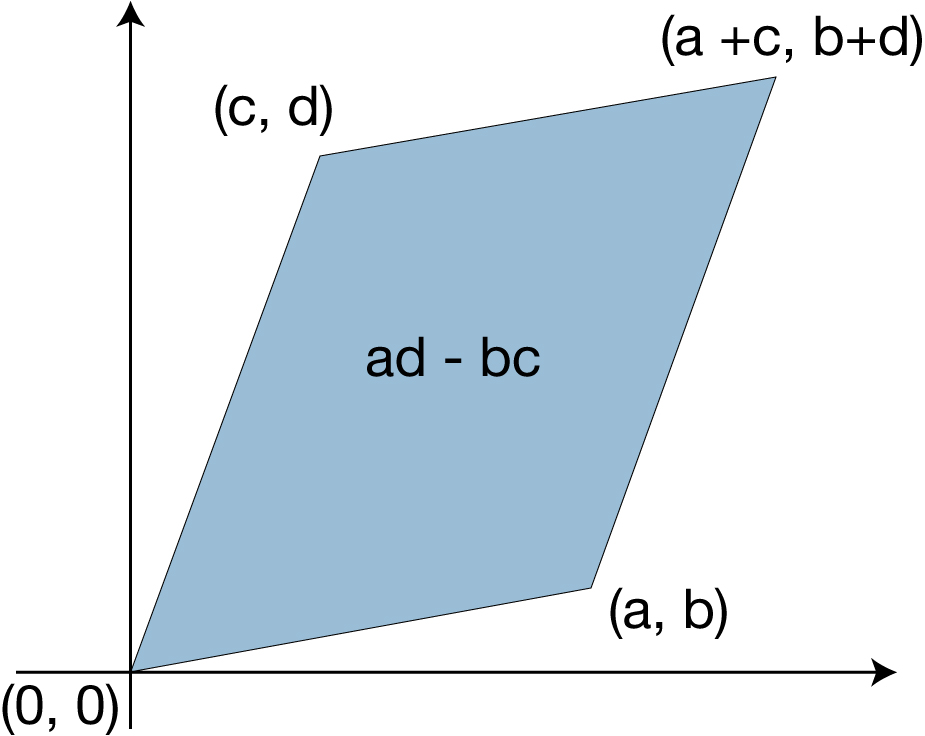
\includegraphics[width=.4\textwidth]{Chapter3/images/image002.jpg} 
    \end{center}
    
    \pause 
    area of parallelogram =  $| \det \spalignmat{a c;b d} | = | ad - bc |$. 

\end{frame}



\begin{frame}\frametitle{Area and Determinants}


 \Emph{Key Geometric Fact (which works in any dimension).} 
 The area of the parallelogram spanned by two vectors $ \vec a, \vec b$ is equal to the area spanned 
by $ \vec a , c\vec a + \vec b$, for any scalar $ c$.   
 
\begin{center}
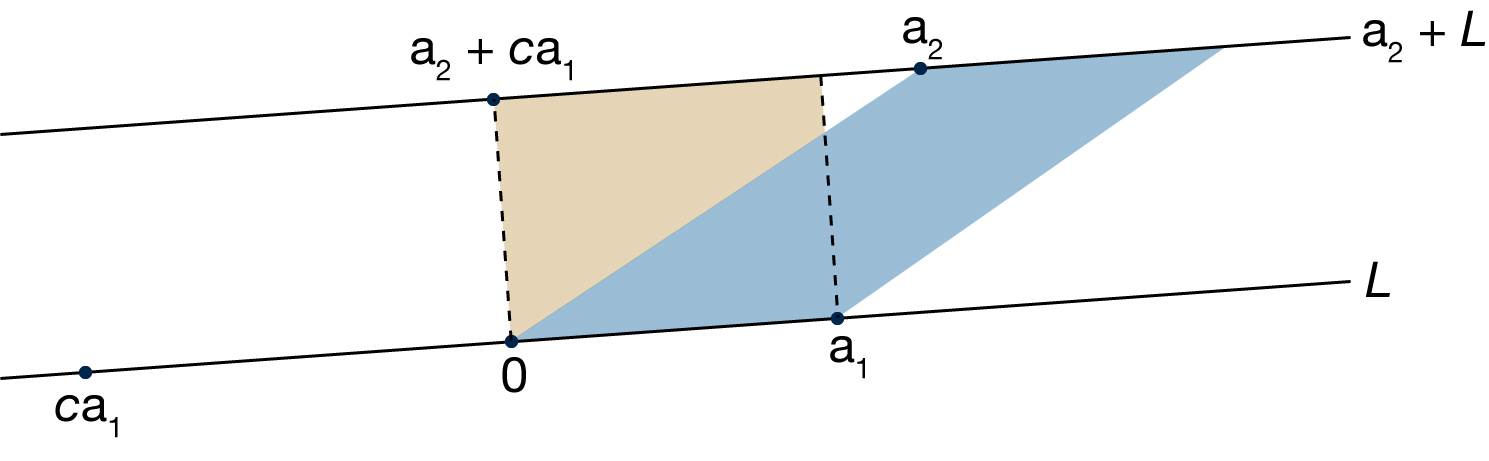
\includegraphics[width=0.7\textwidth]{Chapter3/images/image003.jpg} 
\end{center}

\end{frame}




\begin{frame}\frametitle{Example: Area of a Parallelogram}
    Calculate the area of the parallelogram determined by the points $(-2, -2), (0, 3), (4, -1)  ,(6, 4)$, shown in (a). 
    
    \begin{center}
    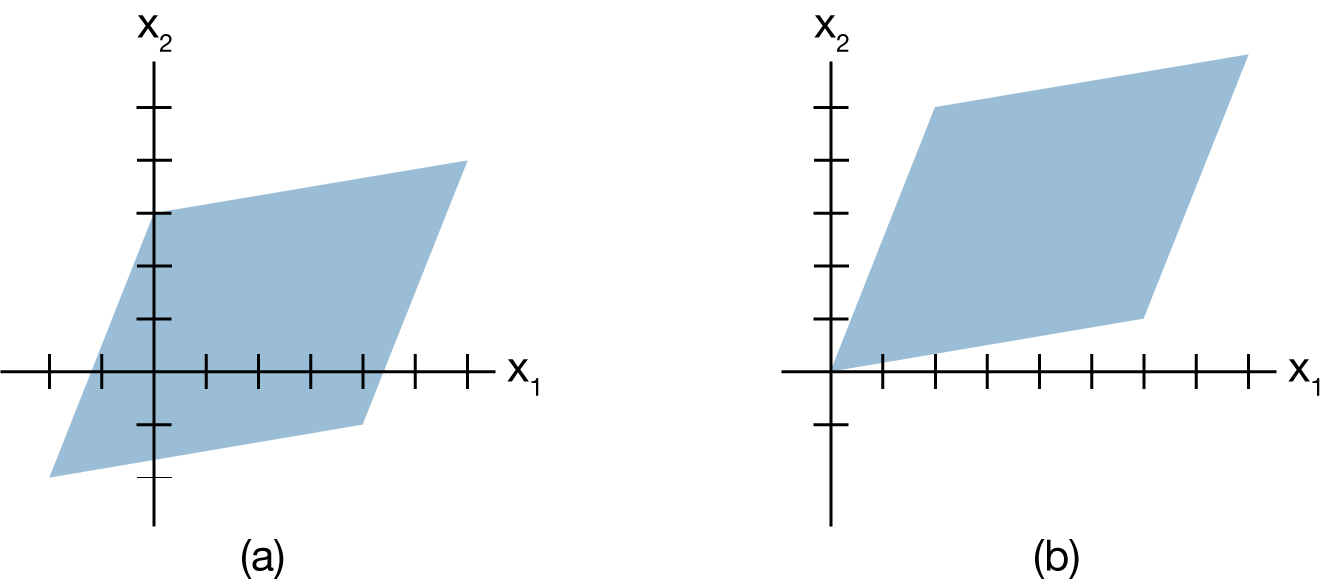
\includegraphics[width=0.6\textwidth]{Chapter3/images/image001.jpg}  
    \end{center}
    
    Note that translating a region in $\mathbb R^2$ does not change its area. 
\end{frame}


\begin{frame}\frametitle{Determinants of $n\times n$ Matrices}

\begin{center}\begin{tikzpicture} \node [mybox](box){\begin{minipage}{0.80\textwidth} \vspace{2pt}

The volume of the parallelpiped spanned by the columns of an $n\times n$ matrix $ A$ is $ \lvert  \operatorname {det} A\rvert $. 

 \end{minipage}}; \node[fancytitle, right=10pt] at (box.north west) {Theorem}; \end{tikzpicture}\end{center}


\end{frame}


\begin{frame}\frametitle{Example: Volume of a Parallelepiped}

    Any $3 \times  3$ matrix $ A$ can be transformed into a diagonal matrix using row operations that do not change 
    $ \lvert  \operatorname {det} (A)\rvert $. 
    
    \vspace{12pt}
    \begin{center}
    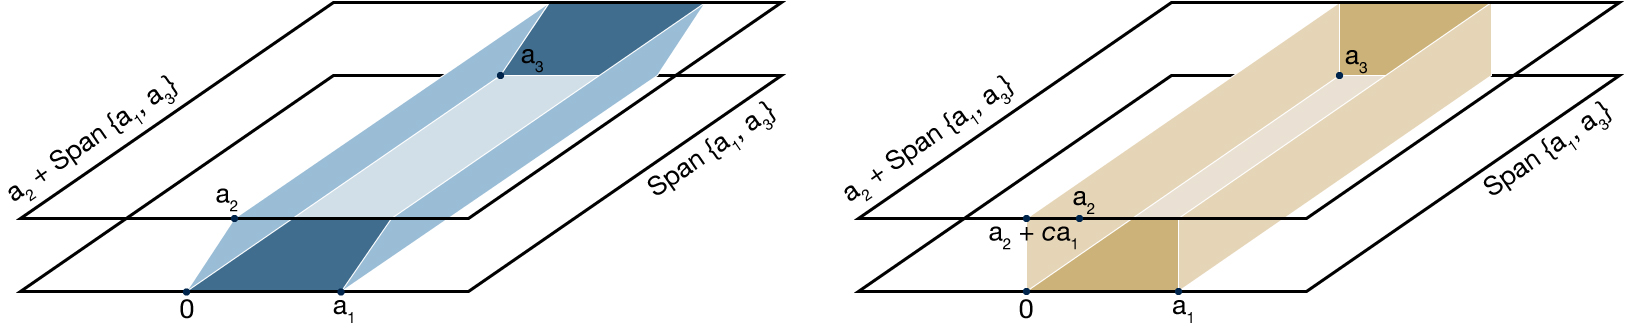
\includegraphics[width=\textwidth]{Chapter3/images/image004.jpg} 
    \end{center}

\end{frame}



\begin{frame}\frametitle{Example: Volume of a Parallelepiped}

    Compute the volume of the parallelepiped that has one vertex at the origin, and adjacent vertices at $(2,0,0)$, $(1,3,0)$, and $(0,1,4)$.  

\end{frame}


\frame{\frametitle{Summary}

    \SummaryLine \vspace{4pt}
    \begin{itemize}\setlength{\itemsep}{8pt}
        \item using determinants to compute the area of a parallelogram, or the volume of a parallelepiped
    \end{itemize}
    
}








     
    % \title{Determinants and Linear Transformations}
\subtitle{\SubTitleName}
\institute[]{\Course}
\author{\Instructor}
\maketitle   


\frame{\frametitle{Topics and Objectives}
\Emph{Topics} \\
\TopicStatement
\begin{itemize}

    \item relationships between area, volume, determinants, and linear transformations
    
\end{itemize}

\vspace{0.5cm}

\Emph{Objectives}\\

\LearningObjectiveStatement

\begin{itemize}

    \item apply determinants to compute the area of a parallelogram, or the volume of a parallelepiped, possibly under a given linear transformation

\end{itemize}

\vspace{0.25cm} 

}



\begin{frame}\frametitle{Linear Transformations}

    \begin{center}\begin{tikzpicture} \node [mybox](box){\begin{minipage}{0.80\textwidth} \vspace{4pt}

    If $T_A \ : \R^n \mapsto \R^n$, and $S$ is some parallelogram in $\R^n$, then $$\operatorname{volume}\left(T_A(S)\right) = \left|\det(A)\right| \cdot \operatorname{volume}(S)$$
    where $T_A (\vec x) = A \vec x$.

    \end{minipage}}; \node[fancytitle, right=10pt] at (box.north west) {Theorem}; \end{tikzpicture}\end{center}


\end{frame}

\begin{frame}\frametitle{Example: Determinants and Linear Transformations}

    $R$ is the parallelogram determined by $\vec p_1 = \spalignmat{3;4}$, and $\vec p_2 = \spalignmat{2;1}$.  If $A = \spalignmat{1 -1;1 1}$, what is the area of the image of $R$ under the map $ \vec x\mapsto A\vec x$? 
    
\end{frame}


\begin{frame}\frametitle{Example: Determinants and Linear Transformations}

    $T_A = A\vec x$, where $A \in \mathbb R^{2\times 2}$, is a linear transformation that first reflects vectors in $\mathbb R^2$ through the line $x_1=x_2$, then projects them onto the line $x_1 = 0$. Calculate the value of the determinant of $A$. 
    


\end{frame}


\frame{\frametitle{Summary}

    \SummaryLine \vspace{4pt}
    \begin{itemize}\setlength{\itemsep}{8pt}
        \item relationships between determinants and linear transformations
    \end{itemize}

}
\frame{

}
     
% \fi



% \ifnum \Week = 8
%     \newcommand{\SubTitleName}{Determinants and Eigenvalues} 
    % \title{Markov Chains and Steady States}
\subtitle{\SubTitleName}
\institute[]{\Course}
\author{\Instructor}
\maketitle   



\frame{\frametitle{Topics and Objectives}
\Emph{Topics} \\
\TopicStatement
\begin{itemize}

    \item Markov chains and probability vectors
    \item steady-state vectors
    % \item convergence

\end{itemize}

\vspace{0.5cm}

\Emph{Objectives}\\

\LearningObjectiveStatement

\begin{itemize}

    \item construct stochastic matrices and probability vectors
    
    \item identify steady-states of Markov chains
    
    % \item model and solve real-world problems using Markov chains (e.g. - find a steady-state vector for a Markov chain)
    
    % \item determine whether a stochastic matrix is regular 
    
\end{itemize}

\vspace{0.25cm} 

}




\begin{frame}\frametitle{A Small Town with Two Libraries}

    \begin{itemize}
        \item A small town has two libraries, $A$ and $B$.
        \item After 1 month, among the books checked out of $A$,
        \begin{itemize}
            \item 80\% returned to $A$
            \item 20\% returned to $B$ 
        \end{itemize}
        \item After 1 month, among the books checked out of $B$,
        \begin{itemize}
            \item 30\% returned to $A$
            \item 70\% returned to $B$ 
        \end{itemize}       
    \end{itemize}
    \pause 
    If both libraries have 1000 books today, how many books does each library have after 1 month? After one year? After $n$ months? 
    % A place to simulate this is \url{http://setosa.io/markov/index.html} 

    \pause 
\vfill 
 
 \begin{center}
 \begin{tikzpicture}
\begin{scope}[->,>=stealth',shorten >=1pt,auto,node distance=3cm,
  thick,main node/.style={circle,fill=DarkBlue!30,draw,font=\sffamily\Large\bfseries}]
   \node[main node] (1) {A};
  \node[main node] (2) [right of=1] {B};
  \path[every node/.style={font=\sffamily\small}]
    (1) edge [bend right] node[below] {0.2} (2)
        edge [loop left] node {0.8} (1)
    (2) edge node [above] {0.3} (1)
        edge [loop right] node {0.7} (2);
\end{scope}
 %\draw (6,0) node {$ \displaystyle P = \begin{bmatrix}.8 & .3 \\ .2 & .7 \end{bmatrix}$ }; 
\end{tikzpicture}    
 \end{center}

    
 
\end{frame}


\begin{frame}\frametitle{Example 1 Continued}

    The books are equally divided by between the two branches, denoted by $\vec x_0 = \begin{bmatrix}
    .5 \\ .5
    \end{bmatrix}$.  What is the distribution after 1 month, call it $\vec x_1$?  After two months? 

    \vspace{2cm}
    
     After $k$ months, the distribution is $\vec x_k$, which is what in terms of $\vec x_0$? 
    
    \vspace{2cm}
    
\end{frame}


\begin{frame}\frametitle{Markov Chains}

    A few definitions: 
    \begin{itemize}
        \item<1-> A \Emph{probability vector} is a vector, $\vec x$, with non-negative elements that sum to 1.
        \item<2-> A \Emph{stochastic matrix} is a square matrix, $P$, whose columns are probability vectors. 
        \item<3-> A \Emph{Markov chain} is a sequence of probability vectors $\vec x_k$, and a stochastic matrix $P$, such that:$$\vec x_{k+1} = P\vec x_k, \quad k = 0, 1, 2, \ldots $$
        \item<4-> A \Emph{steady-state vector} for $P$ is a probability vector $\vec{q}$ such that $P\vec q = \vec q$. 
    \end{itemize}
    
\end{frame}

\begin{frame}\frametitle{Example: Identifying a Steady-State}

    Determine a steady-state vector for the stochastic matrix
    
    $$P = \spalignmat{ .8 .3 ; .2 .7 }$$

\end{frame}

\frame{\frametitle{Summary}

    \SummaryLine \vspace{4pt}
    \begin{itemize}\setlength{\itemsep}{8pt}
        \item Markov chains, stochastic matrices, probability vectors, steady-states
        \item a process to identify steady-states of Markov chains
    \end{itemize}
    
}

    % \title{Markov Chain Convergence}
\subtitle{\SubTitleName}
\institute[]{\Course}
\author{\Instructor}
\maketitle   



\frame{\frametitle{Topics and Objectives}
\Emph{Topics} \\
\TopicStatement
\begin{itemize}

    \item regular stochastic matrices and their relationship to convergence of Markov chains

\end{itemize}

\vspace{0.5cm}

\Emph{Objectives}\\

\LearningObjectiveStatement

\begin{itemize}

    % \item construct stochastic matrices and probability vectors
    
    % \item identify steady-states of Markov chains
    
    \item model and solve real-world problems using Markov chains (e.g. - find a steady-state vector for a Markov chain)
    
    \item determine whether a stochastic matrix is regular 
    
\end{itemize}

\vspace{0.25cm} 

}




\begin{frame}\frametitle{Convergence}

    We often want to know what happens to a process, 
    
    \begin{align}
        \vec x_{k+1} = P\vec x_k, \quad k = 0, 1, 2, \ldots 
    \end{align}
    
    as $k \rightarrow \infty$. 
    
    \vspace{12pt} 
    We may want to know, for example, if the sequence generated by (1),
    $$\vec x_1, \vec x_2, \vec x_3, \ldots$$
    will converge to a steady-state, and if so, what those steady-state vectors are. 
    
\end{frame}



\begin{frame}\frametitle{Regular Stochastic Matrices}

    \begin{center}\begin{tikzpicture} \node [mybox](box){\begin{minipage}{0.85\textwidth}\vspace{4pt}
    
    A stochastic matrix $P$ is \Emph{regular} if there is some $k$ such that $P^k$ only contains strictly positive entries.
    
    \end{minipage}};
    \node[fancytitle, right=10pt] at (box.north west) {Definition};
    \end{tikzpicture}\end{center}
    
    \vspace{12pt}
    \pause 
    
    This matrix is regular stochastic:
    \begin{align*}
        A &= \spalignmat{0.1 0.7;0.9 0.3} = \frac{1}{10} \spalignmat{1 7;9 3} 
    \end{align*}
    
\end{frame}


\begin{frame}\frametitle{Another Example of a Regular Stochastic Matrix}

    Another example of a regular stochastic matrix:
    \begin{align*}
        B & = \frac{1}{10}\spalignmat{0 1 2;2 8 7;8 1 1} 
    \end{align*}
    
    \pause 
    
    Note that
    \begin{align*}
        B^2 & = \frac{1}{100}\spalignmat{18 10 9;72 73 67;10 17 24} 
    \end{align*}
    
    \pause 
    Because $B^k$ has strictly positive entries for $k=2$, $B$ is regular stochastic. 
    
    \vspace{6pt}
    \pause
    It can be very difficult to determine whether a matrix is regular stochastic. 
\end{frame}



\begin{frame}\frametitle{Convergence and Regular Stochastic Matrices}

    \begin{center}\begin{tikzpicture} \node [mybox](box){\begin{minipage}{0.85\textwidth}\vspace{4pt}
    
    If $P$ is a regular stochastic matrix, then $P$ has a unique steady-state vector $\vec q$, and $\vec x_{k+1} = P\vec x_k$ converges to $\vec q$ as $k \rightarrow \infty$. 
    
    \end{minipage}};
    \node[fancytitle, right=10pt] at (box.north west) {Theorem};
    \end{tikzpicture}\end{center}

\end{frame}


\begin{frame}\frametitle{Example: Car Rental Company}

    A car rental company has 3 rental locations, A, B, and C. Cars can be returned at any location. The table below gives the pattern of rental and returns for a given week.
    
    \begin{table}[]
    \centering
    \label{my-label}
    \begin{tabular}{lllll}
                      &  & \multicolumn{3}{l}{rented from} \\\hline
                      &  & A & B & C \\\hline
    \multirow{3}{*}{returned to} & A & .8 & .1  & .2  \\
                      & B & .2 & .6 & .3     \\
                      & C & .0 & .3 & .5   \\\hline
    \end{tabular}
    \end{table}
        
     There are 1000 cars at each location today. 
     \begin{enumerate}[a)]
        \item Construct a stochastic matrix, $P$, for this problem.
        \item What happens to the distribution of cars after a long time? You may assume that $P$ is regular. 
     \end{enumerate}

\end{frame}




%% FRAME
\begin{frame}\frametitle{Solution to Part (a): Set of Equations}
    \begin{table}[]
    \begin{tabular}{lllll}
                      &  & \multicolumn{3}{l}{rented from} \\\hline
                      &  & A & B & C \\\hline
    \multirow{3}{*}{returned to} & A & .8 & .1  & .2  \\
                      & B & .2 & .6 & .3     \\
                      & C & .0 & .3 & .5   \\\hline
    \end{tabular}
    \end{table}
    
    \pause 
    
    If $x_{A,k}, x_{B,k}, x_{C,k}$ are the number of cars in week $k$ at locations $A,B,C$ respectively, then after one week,
    \begin{align*}
        \onslide<2->{x_{A,1} & = 0.8x_{A,0} + 0.1x_{B,0} + 0.2x_{C,0} \\ }
        \onslide<3->{x_{B,1} & = 0.2x_{A,0} + 0.6x_{B,0} + 0.3x_{C,0}  \\ }
        \onslide<4->{x_{C,1} & = 0.0x_{A,0} + 0.3x_{B,0} + 0.5x_{C,0} }
    \end{align*}
    
\end{frame}

\begin{frame}\frametitle{Solution to Part (a): Matrix $P$}

    Our set of equations can be represented with a matrix equation, \pause
        \begin{align*}
        x_{A,1} & = 0.8x_{A,0} + 0.1x_{B,0} + 0.2x_{C,0} \\ 
        x_{B,1} & = 0.2x_{A,0} + 0.6x_{B,0} + 0.3x_{C,0} \quad \Rightarrow \quad \vec x_1 = P\vec x_0 \\
        x_{C,1} & = 0.0x_{A,0} + 0.3x_{B,0} + 0.5x_{C,0} 
    \end{align*}
    where
    \pause 
    $$P = \begin{pmatrix}
.8 & .1 & .2 \\ .2 & .6 & .3 \\ .0 & .3 & .5 
\end{pmatrix}
$$
\end{frame}




%% FRAME
\begin{frame}\frametitle{Solution to Part (a): Another Perspective}
    Another approach to determining $P$ involving a graph. 
    
    \vspace{12pt}
    
    \begin{tikzpicture}
    \begin{scope}[->,>=stealth',shorten >=1pt,auto,node distance=3.5cm,
      thick,main node/.style={circle,fill=DarkBlue!10,draw,font=\sffamily\bfseries}]
      \node[main node] (1) {A};
      \node[main node] (2) [right of=1] {B};
        \node[main node] (3) [below right of=1] {C};
      \path[every node/.style={font=\sffamily\small}]
        (1) edge [bend right] node[below] {.2} (2)
            edge [loop left] node {.8} (1)
        (2) edge node [above] {.1} (1)
            edge [loop right] node {.6} (2)
            edge [left] node {.3}  (3) 
         (3) edge node [bend left] {.2} (1)
            edge [loop below] node {.5} (3)
            edge [bend right] node[right] {.3}  (2);
    \end{scope}
    \draw (7,-1) node {
    $ \displaystyle 
    P = 
    \begin{pmatrix}
    .8 & .1 & .2 \\ .2 & .6 & .3 \\ .0 & .3 & .5 
    \end{pmatrix}
    $ }; 
        \end{tikzpicture}    

\end{frame}

\begin{frame}\frametitle{Solution to Part (b)}

    Part b: \textit{What happens to the distribution of cars after a long time? You may assume that $P$ is regular. }
    
    
    \vspace{12pt}
    \onslide<2->{$P$ is regular $\Rightarrow$ can assume that $P$ has a unique steady-state vector $\vec q$, and $\vec x_{k+1} = P\vec x_k$ converges to $\vec q$ as $k \rightarrow \infty$. }
    
    \vspace{12pt}
    \onslide<3->{The steady-state vector, $\vec q$ is given by: }
    \begin{align*}
        \onslide<4->{P\vec q &= \vec q \\}
        \onslide<5->{P\vec q - \vec q &= \vec 0 \\}
        \onslide<6->{(P - I)\vec q &= \vec 0 }
    \end{align*}
    \onslide<7->{$\vec q$ is a probability vector in Null$(P-I)$. We need to calculate $P-I$ and $\vec q \ldots $}
\end{frame}

\frame{
$$P-I = \begin{pmatrix}
    .8 -1 & .1 & .2 \\ .2 & .6-1 & .3 \\ .0 & .3 & .5 -1
    \end{pmatrix} = \begin{pmatrix}
    -.2 & .1 & .2 \\ .2 & -.4 & .3 \\ .0 & .3 & -.5
    \end{pmatrix}
    $$
    \pause
$\vec q$ is a vector in the null space of the above matrix. We apply the usual process for finding a vector in the null space of a matrix. 
\pause
    \begin{align*}
        \spalignaugmat{-.2 .1 .2 0;.2 -.4 .3 0 ; 0 .3 -.5 0} \sim \spalignaugmat{-2 1 2 0;0 -3 5 0 ; 0 3 -5 0} \sim \spalignaugmat{6 0 -11 0;0 -3 5 0 ; 0 0 0 0}
    \end{align*}
    $x_3$ is free. If we set $x_3 = 6$, then 
    \pause 
    \begin{align*}
        6x_1 -11x_3 = 0 &\Rightarrow x_1 = 11 \\
        -3x_2 +5x_3 = 0 &\Rightarrow x_2 = 10
    \end{align*}
    Therefore ... 
}    
\frame{    
    A vector in the null space of $P-I$ is 
    \pause
    $$\spalignmat{11;10;6}$$
    \pause
    A probability vector in the null space is
    $$\vec q = \frac{1}{27} \spalignmat{11;10;6}$$
    This is our steady-state vector. 
    
    \vspace{12pt}
    \pause
    No matter what the initial distribution of cars happens to be, after a long period of time, the distribution of cars is given by $\vec q$. 
}

% \begin{frame}\frametitle{Convergence in $\mathbb R^2$}
%     The stochastic vectors in the plane are  the line segment below, and a stochastic matrix maps stochastic vectors to themselves. Iterates $ P ^{k} \vec x_0$ converge to the steady state. 
    
%     \vspace{12pt} 
    
%     \begin{tikzpicture}[scale=0.9]
%     \draw[->] (-0.5,0) -- (4,0);  \draw[->] (0,-0.5) -- (0,4); 
%     \draw (3,0) node[below] {1} -- (0,3) node[left] {1};  
%     \filldraw  (2,1) circle (.1em) node (S) {}; 
%     \draw[<<-] (2,1) node[below,left] {$\color{DarkRed} \vec x _{\infty }$}  --  (4,2) node [above] {Steady State Vector}; 
%     \foreach \x/\y/\k in { 3/0/0 , 1/2/1, 2.5/0.5/2, 1.5/1.5/3} \filldraw (\x,\y) circle (0.1em) node[above] {$ \vec x_{\k}$}; 
%     \draw (8,1) node {  $ P ^{k} \longrightarrow \begin{bmatrix}
%     \vec x _{\infty } & \vec x _{\infty }
%     \end{bmatrix}$}; 
%     \end{tikzpicture}
% \end{frame} 

% \begin{frame}\frametitle{Convergence in $\mathbb R^3$}
% The Stochastic vectors in $ \mathbb R ^{3}$, are vectors $ \begin{bmatrix}
% s \\ t \\ 1- s-t 
% \end{bmatrix}$, where $ 0 \leq s , t \leq 1$ and $ s+t \leq 1$.  $ P$ \Emph{contracts} stochastic vectors to $\vec x _{\infty }$. 


% \begin{center}
% \begin{tikzpicture}[scale=0.9]
% \draw (0,3.5) node[above] {$ (1,0,0)$} --  (3,0) node[below] {$ (0,1,0)$} -- 
%  (-3,0) node[below] {$ (0,0,1)$} --  (0,3.5);  
% \filldraw (1,1) circle (.15em) node[above] {$\color{DarkRed} \vec x _{\infty }$}; 
% \end{tikzpicture}
% \end{center}
% \end{frame}
    
    
\frame{\frametitle{Summary}

    \SummaryLine \vspace{4pt}
    \begin{itemize}\setlength{\itemsep}{8pt}
        \item regular stochastic matrices and their relationship to convergence of Markov chains
    \end{itemize}
    % Later in our course we will take another look at Markov chains and their relationship to eigenvalue problems and other applications. 
    
}

\frame{

}
    % \title{Eigenvalues and Eigenvectors}
\subtitle{\SubTitleName}
\institute[]{\Course}
\author{\Instructor}
\maketitle   

\frame{\frametitle{Topics and Objectives}
    \Emph{Topics} \\
    \TopicStatement
    \begin{itemize}

        \item eigenvectors, eigenvalues %, eigenspaces
        % \item Eigenvalue theorems

    \end{itemize}

    \vspace{0.5cm}

    \Emph{Objectives}\\

    \LearningObjectiveStatement

    \begin{itemize}

        \item determine whether a given vector is an eigenvector of a given matrix

        \item determine whether a given number is an eigenvalue of a given matrix
        
        % \item Construct an eigenspace for a matrix.
        
        % \item Apply theorems related to eigenvalues (for example, to characterize the invertibility of a matrix).

    \end{itemize}
}


\begin{frame}{Motivating Problem}

    Consider the linear transform 
        $$T_A(\vec x) = A \vec x = \spalignmat{0 1;1 0} \spalignmat{x_1;x_2}.$$

    \pause 
    
    Can you state a non-zero vector, $\vec v \in \mathbb R^2$ that satisfies the following equation? 
    
    $$A \vec v = \lambda \vec v, \quad \lambda \in \mathbb R$$
    

    \pause 
    \begin{tikzpicture}[scale=1.2]
    
        \coordinate (O) at (0,0);  % variable for origin
              
        % axes
        \draw[-, thin,black] (-1.25,0) -- (1.5,0) node[anchor=west] {$x_1$};
        \draw[-, thin,black] (0,-0.7) -- (0.0,1.75) node[anchor=east] {$x_2$};
        
        % reflection line
        \draw[-,thick,Teal](-.7,-.7)--(1.5,1.5) node[anchor=south] {$x_2=x_1$};
        
    \end{tikzpicture}

\end{frame}


\begin{frame}{Eigenvectors and Eigenvalues}

    If $A \in \R^{n\times n}$, and there is a $\vec v \neq \vec 0$ in $\R^n$, and
        \[ A\vec v=\lambda \vec v \]
    then \onslide<2->{ $\vec v$ is an \Emph{eigenvector} for $A$, and $\lambda \in \mathbb C$ is the corresponding \Emph{eigenvalue}.} 

    \vspace{12pt}
    
    \onslide<2->{Note that}
    \begin{itemize}
        \item<3-> we will only consider the case where $A$ is square
        \item<4-> even when all entries of $A$ and $\vec v$ are real, $\lambda$ can be complex
        (a rotation of the plane has no \Emph{real} eigenvalues.) 
        \item<5-> if $\lambda \in \mathbb R$, then
        \begin{itemize}
            \item when $\lambda > 0$, $A\vec v$ and $\vec v$ point in the same direction
            \item when $\lambda < 0$, $A\vec v$ and $\vec v$ point in opposite directions
        \end{itemize}    \end{itemize}


\end{frame}



\begin{frame}{Determining Whether a Vector is an Eigenvector}

    Which of the following vectors are eigenvectors of $A=\spalignmat{ 1 1 ; 1 1}$? 

    \begin{enumerate}[a)]
        \item $\vec v_1 = \spalignmat{1;1}$ 
        \item $\vec v_2 = \spalignmat{2;2}$ 
        \item $\vec v_3 = \spalignmat{1;-1}$ 
        \item $\vec v_4 = \spalignmat{2;1}$ 
        \item $\vec v_5 = \spalignmat{0;0}$
    \end{enumerate}

\end{frame}


\begin{frame}{Determining Whether a Number is an Eigenvalue}

    Determine whether $\lambda =3$ is an eigenvalue of $A=\spalignmat{2 -4 ; -1 -1}$. 


\end{frame}


\begin{frame}{Another Interpretation of What Eigenvalues Are}

    From the previous examples, we saw how an eigenvalue of a matrix is a number, $\lambda$, that
    
    \pause 
    \begin{itemize}
        \item satisfies $A\vec v = \lambda \vec v$ for eigenvector $\vec v$
        \item makes $A - \lambda I$ singular
    \end{itemize}

    \pause 
    Recall: a singular matrix is not invertible. 

\end{frame}



\frame{\frametitle{Summary}

    \SummaryLine \vspace{4pt}
    \begin{itemize}\setlength{\itemsep}{8pt}
        \item the definitions of eigenvectors and eigenvalues %, eigenspaces

        \item determine whether a given vector is an eigenvector of a given matrix

        \item determine whether a given number is an eigenvalue of a given matrix
    \end{itemize}
    \vspace{8pt}
    Later in our course we will take explore ways to compute the eigenvalues and eigenvectors of a matrix, as well as some of their applications. 
    
}
















    % \title{Eigenspaces}
\subtitle{\SubTitleName}
\institute[]{\Course}
\author{\Instructor}
\maketitle   

\frame{\frametitle{Topics and Objectives}
    \Emph{Topics} \\
    \TopicStatement
    \begin{itemize}

        \item eigenspaces
        % \item Eigenvalue theorems

    \end{itemize}

    \vspace{0.5cm}

    \Emph{Objectives}\\

    \LearningObjectiveStatement

    \begin{itemize}

        \item construct and sketch the eigenvectors for a matrix given its eigenvalues
        
        \item construct and sketch an eigenspace for a matrix
        
        % \item Apply theorems related to eigenvalues (for example, to characterize the invertibility of a matrix).

    \end{itemize}
}






\begin{frame}{Eigenspaces}

    % ~~ ~~ Highlight Box ~~ ~~
    \begin{center}\begin{tikzpicture} \node [mybox](box){\begin{minipage}{0.80\textwidth}\vspace{2pt}

        Suppose $A \in \R^{n \times n}$. The eigenvectors for a given $\lambda$ span a subspace of $\R^n$ called the $\lambda$-\Emph{eigenspace} of $A$.

    \end{minipage}};
    \node[fancytitle, right=10pt] at (box.north west) {Definition};
    \end{tikzpicture}\end{center}
    % ~~ ~~ Highlight Box ~~ ~~

    \vspace{2pt} 

    \Emph{Note:} the $\lambda$-eigenspace for matrix $A$ is $\textrm{Nul} (A-\lambda I)$, because: \pause 
    \begin{align*}
        A \vec v & = \lambda \vec v \\
        A \vec v - \lambda I \vec v & = \vec 0 \\
        (A - \lambda I) \vec v &= \vec 0
    \end{align*}
    \pause If $\vec v \ne 0$, we must have that $A - \lambda I$ is singular. \pause Thus, eigenvectors span the null space of $A - \lambda I$. 
\end{frame}



\begin{frame}{Eigenspaces in $\mathbb R^2$}

    Construct a basis for the eigenspaces for the matrix whose eigenvalues are given. Sketch the eigenvectors and eigenspaces. $$A = \spalignmat{ 5 -6; 3 -4}, \quad \lambda = -1, 2$$

\end{frame}



\begin{frame}{Eigenspaces in $\mathbb R^3$}

    Construct a basis for the eigenspaces for the matrix whose eigenvalues are given. $$A= \spalignmat{ 3 0 0;0 2 1;0 1 2}, \quad \lambda = 1, 3$$

\end{frame}




\frame{\frametitle{Summary}

    \SummaryLine \vspace{4pt}
    \begin{itemize}\setlength{\itemsep}{8pt}

        \item constructing the eigenvectors for a matrix given its eigenvalues
        
        \item constructing an eigenspace for a matrix
        
    \end{itemize}
    \vspace{8pt}

}








    % \title{Eigenvalue Theorems}
\subtitle{\SubTitleName}
\institute[]{\Course}
\author{\Instructor}
\maketitle   

\frame{\frametitle{Topics and Objectives}
    \Emph{Topics} \\
    \TopicStatement
    \begin{itemize}

        % \item eigenspaces
        \item eigenvalue theorems

    \end{itemize}

    \vspace{0.5cm}

    \Emph{Objectives}\\

    \LearningObjectiveStatement

    \begin{itemize}

        
        % \item construct an eigenspace for a matrix
        
        \item apply theorems related to eigenvalues to characterize matrices and compute eigenvalues

    \end{itemize}
}



\begin{frame}{Motivating Questions}

    Suppose $A$ is a real $n\times n$ matrix. 
    
    \begin{itemize}
        \item<2-> How can we determine the eigenvalues of $A$? 
        \item<3-> If $A$ has some special structure (e.g. - singular, stochastic, triangular), what can we say about the eigenvalues of $A$? 
    \end{itemize}
    
    \onslide<4->{Theorems that deal with eigenvalues of a matrix can help us calculate eigenvalues. }
    
\end{frame}




\begin{frame}{Theorems}

    The following theorems can help us identify eigenvalues and eigenvectors of a matrix. 
    
    \vspace{12pt}
    
    \begin{itemize}
        \item<2-> The diagonal elements of a triangular matrix are its eigenvalues. \vspace{0.25cm}
        \item<3-> $A$ not invertible $\Leftrightarrow 0$ is an eigenvalue of $A$. \vspace{0.5cm}
        \item<4-> Stochastic matrices have an eigenvalue equal to 1.\vspace{0.5cm}
        \item<5-> If $\vec v_1, \vec v_2, \ldots , \vec v_k$ are eigenvectors that correspond to distinct eigenvalues, then $\vec v_1, \vec v_2, \ldots , \vec v_k$ are linearly independent.
    \end{itemize}
    
    \onslide<6->{Proofs of these theorems are relatively short.}\onslide<7->{There are many other eigenvalue theorems that we could explore!}
    
\end{frame}




\begin{frame}{Determining Eigenvalues by Inspection} 

    By inspection, give two eigenvalues for each of the following matrices.
    \begin{enumerate}
        \item $A=\frac 12 \spalignmat{1 1;1 1}$
        \item $B=\spalignmat{2 3;0 5}$
    \end{enumerate}


\end{frame}




\begin{frame}{\Emph{Warning!}} 

	\vspace{-12pt}
    % ~~ ~~ Highlight Box ~~ ~~
    \begin{center}\begin{tikzpicture} \node [mybox](box){\begin{minipage}{0.94\textwidth}\vspace{4pt}

        We cannot determine the eigenvalues of a matrix from its reduced form. 

    \end{minipage}};
    \end{tikzpicture}\end{center}
    % ~~ ~~ Highlight Box ~~ ~~
    
    In other words: row reductions can change the eigenvalues of a matrix. 
    
\end{frame}




\begin{frame}{Row Operations on $A$ Can Change its Eigenvalues} 

    Suppose $A = \spalignmat{1 1;1 1}$. The eigenvalues and corresponding eigenvectors are 
    
    $$\lambda_1 = 2, \ \vec v_1 = \spalignmat{1;1}, \qquad \lambda_2 = 0, \ \vec v_2 = \spalignmat{1;-1} $$
    
    We can verify this:
    \pause 
            \begin{align*}
            & A \vec v_1
            = \spalignmat{1 1;1 1} 
            \spalignmat{1;1} =  \spalignmat{2;2} = 2 \vec v_1\\
            & A \vec v_2
            = \spalignmat{1 1;1 1} 
            \spalignmat{1;-1} =  \spalignmat{0;0} = 0\vec v_2
            \end{align*}

    \pause
    
    But the RREF of $A$ is $\spalignmat{1 1;0 0}$, whose eigenvalues are $1$ and $0$. 

\end{frame}


\frame{\frametitle{Summary}

    \SummaryLine \vspace{4pt}
    \begin{itemize}\setlength{\itemsep}{8pt}

        \item applying eigenvalue theorems to characterize matrices and compute eigenvalues
        
    \end{itemize}
    \vspace{8pt}

}








    % \title{The Characteristic Polynomial}
\subtitle{\SubTitleName}
\institute[]{\Course}
\author{\Instructor}
\maketitle   



\frame{\frametitle{Topics and Objectives}
\Emph{Topics} \\
\TopicStatement
\begin{itemize}

    \item the characteristic polynomial of a matrix

    % \item Algebraic and geometric multiplicity of eigenvalues

    % \item Similar matrices

\end{itemize}

\vspace{0.5cm}

\Emph{Objectives}\\

\LearningObjectiveStatement

\begin{itemize}

    \item construct the characteristic polynomial of a matrix and use it to identify eigenvalues and their multiplicities
    \item apply the trace and determinant of a $2\times2$ matrix to determine eigenvalues
    % \item characterize the long-term behaviour of dynamical systems using eigenvalues

\end{itemize}

\vspace{0.25cm} 

}




\begin{frame}{The Characteristic Polynomial}

    \Emph{Recall:}
	\vspace{-2pt}
    % ~~ ~~ Highlight Box ~~ ~~
    \begin{center}\begin{tikzpicture} \node [mybox](box){\begin{minipage}{0.7\textwidth}\vspace{2pt}

        \begin{center}
           $\lambda$ is an eigenvalue of $A \ \Leftrightarrow \ (A-\lambda I)$ is not invertible
        \end{center}

    \end{minipage}};
    \end{tikzpicture}\end{center}
    % ~~ ~~ Highlight Box ~~ ~~
    

Therefore, to calculate the eigenvalues of $A$, we can solve
\[ 
\det(A-\lambda I)= 0
\]

\pause

\begin{itemize}
    \item $\det(A-\lambda I)$ is the \Emph{characteristic polynomial} of $A$
    \item $\det(A-\lambda I)=0$ is the  \Emph{characteristic equation} of $A$
    \item the roots of the characteristic polynomial are the eigenvalues of $A$
\end{itemize}



\end{frame}

\begin{frame}{Example: Calculating the Eigenvalues of a $2\times2$ Matrix}

The characteristic polynomial of $A = \spalignmat{ 4 2 ; 2 1} $ is: 

\vspace{2cm}

So the eigenvalues of $A$ are:

\end{frame}




\begin{frame}{Characteristic Polynomial of $2 \times 2$ Matrices}

    The \Emph{trace} of a matrix is the sum of its diagonal elements. 
    
    \vspace{12pt}
    
    \Emph{Example} \\ Express the characteristic equation of
    \begin{align*}
       M = \spalignmat{ a b ; c d }
    \end{align*}
    
    in terms of its determinant and trace. 

\end{frame}





\begin{frame}{Using the Trace to Identify Eigenvalues}

    Although the characteristic polynomial can always be used to determine eigenvalues, sometimes we can identify eigenvalues by inspection.
    
    \vspace{12pt}
    
    \Emph{Example} \\ By inspection, what are the eigenvalues of $A$? 
    $$A = \spalignmat{6 18;3 9}$$

    

\end{frame}




\begin{frame}\frametitle{Numerical Notes}

    \begin{itemize}
        
        \item The eigenvalues of any matrix larger than $2\times2$ should be found using a computer, unless the matrix has a special structure.
        
        \item Software for computing computing eigenvalues tends to avoid the characteristic polynomial.
        
        \item Nevertheless, the characteristic polynomial is important for theoretical purposes. 
    
    \end{itemize}
\end{frame}



\frame{\frametitle{Summary}

    \SummaryLine \vspace{4pt}
    \begin{itemize}\setlength{\itemsep}{8pt}

        \item the characteristic polynomial of a matrix and its use to calculate eigenvalues

    \end{itemize}
    \vspace{8pt}

}











    % \title{Algebraic and Geometric Multiplicities}
\subtitle{\SubTitleName}
\institute[]{\Course}
\author{\Instructor}
\maketitle   



\frame{\frametitle{Topics and Objectives}
\Emph{Topics} \\
\TopicStatement
\begin{itemize}

    % \item the characteristic polynomial of a matrix

    \item the algebraic and geometric multiplicity of eigenvalues

    % \item Similar matrices

\end{itemize}

\vspace{0.5cm}

\Emph{Objectives}\\

\LearningObjectiveStatement

\begin{itemize}

    \item calculate algebraic and geometric multiplicities
    \item construct matrices that have eigenvalues with a given algebraic and/or geometric multiplicity

\end{itemize}

\vspace{0.25cm} 

}



\begin{frame}{Algebraic Multiplicity}

    % ~~ ~~ Highlight Box ~~ ~~
    \begin{center}\begin{tikzpicture} \node [mybox](box){\begin{minipage}{0.85\textwidth}\vspace{2pt}

        The \Emph{algebraic multiplicity} of an eigenvalue is its multiplicity as a root of the characteristic polynomial.

    \end{minipage}};
    \node[fancytitle, right=10pt] at (box.north west) {Definition};
    \end{tikzpicture}\end{center}
    % ~~ ~~ Highlight Box ~~ ~~
    
    \Emph{Example} \\ Compute the algebraic multiplicities of the eigenvalues for the matrix
    \[ \spalignmat{ 1 0 0 0 ; 0 0 0 0 ; 0 0 -1 0 ; 0 0 0 0 } \]


\end{frame}




\begin{frame}{Geometric Multiplicity}

    % ~~ ~~ Highlight Box ~~ ~~
    \begin{center}\begin{tikzpicture} \node [mybox](box){\begin{minipage}{0.85\textwidth}\vspace{2pt}

        The \Emph{geometric multiplicity} of an eigenvalue $\lambda$  is  the dimension of $ \operatorname{Null} (A - \lambda I)$. 

    \end{minipage}};
    \node[fancytitle, right=10pt] at (box.north west) {Definition};
    \end{tikzpicture}\end{center}
    % ~~ ~~ Highlight Box ~~ ~~
    \vspace{-6pt}
    \begin{itemize}
        \item  Geometric multiplicity is always at least 1.  It can be smaller than algebraic multiplicity. 
        
        \item  Here is the basic example:  
         \[ \spalignmat{ 0 1 ; 0 0 } \]
         $\lambda =0$ is the only eigenvalue. Its algebraic multiplicity is 2, but the geometric multiplicity is 1.  
    \end{itemize}

\end{frame}




\begin{frame}{Properties of Algebraic and Geometric Multiplicities}

    Suppose that, for an $n\times n$ matrix $A$,
    \begin{itemize}
        \item $a_i$ is the algebraic multiplicity of $\lambda_i$
        \item $g_i$ is the geometric multiplicity of $\lambda_i$
    \end{itemize}
    
    \pause 
    
    \vspace{12pt}
    The algebraic and geometric multiplicities have the following properties. 
    \begin{itemize}
        \item $1 \le a_i \le n$
        \item $1 \le g_i \le a_i$
    \end{itemize}
    
\end{frame}




\begin{frame}{Example}

    Give an example of a $4\times 4$ matrix with $\lambda =0$ the only eigenvalue, but the geometric multiplicity of $\lambda=0$ is one. 

\end{frame}

\begin{frame}{Example: Algebraic Multiplicity}

    For what values of $k$ does the matrix have one real eigenvalue with algebraic multiplicity 2? 
    
    $$\spalignmat{-3 k; 2 -6}$$

\end{frame}


\frame{\frametitle{Summary}

    \SummaryLine \vspace{4pt}
    \begin{itemize}\setlength{\itemsep}{8pt}

        \item the algebraic and geometric multiplicity of eigenvalues
        \item constructing matrices that have eigenvalues with given algebraic or geometric multiplicities

    \end{itemize}
    \vspace{8pt}

}











    % \title{Markov Chains and Eigenvectors}
\subtitle{\SubTitleName}
\institute[]{\Course}
\author{\Instructor}
\maketitle   



\frame{\frametitle{Topics and Objectives}
\Emph{Topics} \\
\TopicStatement
\begin{itemize}

    \item the use of eigenvalues and eigenvectors to study Markov chains

\end{itemize}

\vspace{0.5cm}

\Emph{Objectives}\\

\LearningObjectiveStatement

\begin{itemize}

    \item apply eigenvalues and eigenvectors to characterize the long-term behavior of Markov chains

\end{itemize}

\vspace{0.25cm} 

}


\begin{frame}{The Long-Term Behavior of Markov Chains}

    \begin{itemize}
        \item recall that we often want to know what happens to a Markov chain $$\vec x_{k+1} = P\vec x_k, \quad k = 0, 1, 2, \ldots $$ as $k \rightarrow \infty$
        \item if $P$ is a regular stochastic matrix there will be a unique steady-state
   \end{itemize}

    \vspace{6pt} 
    
    \pause 
    
    Now we can explore the following questions.
    \begin{itemize}
        \item if we do not know whether $P$ is regular, what else might we do to describe the long-term behavior of the system? 
        \item What can eigenvalues tell us about the behavior of these systems?
    \end{itemize}
\end{frame}





\begin{frame}{Example: Eigenvalues and Markov Chains}


    Consider the Markov Chain: $$\vec x_{k+1} = P\vec x_{k} = \spalignmat{1 0.1 ;0 0.9 }\vec x_{k}, \quad k= 0, 1, 2, 3, \ldots, \quad \vec x_0 = \spalignmat{0;1}.$$

    \pause 
    
    This system can be represented schematically with two nodes, A and B: 
    
    \vspace{-6pt} 
    
    \begin{center}
    \begin{tikzpicture}
    \begin{scope}[->,>=stealth',shorten >=1pt,auto,node distance=3cm, thick,main node/.style = {circle,fill=DarkBlue!30,draw,font=\sffamily\Large\bfseries}]
    \node[main node] (1) {A};
    \node[main node] (2) [right of=1] {B};
    \path[every node/.style={font=\sffamily\small}]
    (1) edge [loop left] node {1} (1)
    (2) edge node [above] {0.1} (1)
        edge [loop right] node {0.9} (2);
        \end{scope}
        \end{tikzpicture}
    \end{center}
    
    \vspace{-6pt} 
    
    \pause

    \Emph{Goal}: use eigenvalues to describe the long-term behavior of our system. 
    
\end{frame}





\begin{frame}{Example: Eigenvalues and Markov Chains}

    Consider the Markov Chain: $$\vec x_{k+1} = P\vec x_{k} = \spalignmat{1 0.1 ;0 0.9 }\vec x_{k}, \quad k= 0, 1, 2, 3, \ldots, \quad \vec x_0 = \spalignmat{1;0}.$$

    Use the eigenvalues and eigenvectors of $P$ to determine what $\vec x_k$ tends to as $k\to\infty$. The eigenvalues and eigenvectors of $P$ are
    
    $$\lambda_1 = 1, \ \vec v_1 = \spalignmat{1;0}, \quad \lambda_2 = 0.9, \ \vec v_2 = \spalignmat{1;-1}$$
    
    
 
    
    
\end{frame}



\begin{frame}{A More General Example}

    The eigenvalues of a $3\times 3$ stochastic matrix $A$ are 
    $$\lambda_1 = 1 , \quad \lambda_2=\frac{1}{4}, \quad \lambda_3 = \frac 18$$
    The respective eigenvectors corresponding to these eigenvalues are $\vec v_1$, $\vec v_2$, $\vec v_3$. 
    
    \vspace{12pt}
    
    If $\vec p$ is a probability vector in $\mathbb R^3$, what does $A^k\vec p $ tend to as $k\to \infty$? 

\end{frame}



\frame{\frametitle{Summary}

    \SummaryLine \vspace{4pt}
    \begin{itemize}\setlength{\itemsep}{8pt}

        \item using eigenvalues and eigenvectors to study the long-term behavior of Markov chains

    \end{itemize}
    \vspace{8pt}
    
}




\begin{frame}
\end{frame}
    % \title{Similar Matrices}
\subtitle{\SubTitleName}
\institute[]{\Course}
\author{\Instructor}
\maketitle   



\frame{\frametitle{Topics and Objectives}

    \Emph{Topics} \\
    \TopicStatement
    \begin{itemize}
    
        \item similar matrices
    
    \end{itemize}
    
    \vspace{0.5cm}
    
    \Emph{Objectives}\\
    
    \LearningObjectiveStatement
    
    \begin{itemize}
    
        \item apply the definition of similar matrices to determine whether mathematical statements that involve similar matrices are accurate
    
    \end{itemize}

}



\begin{frame}{Motivation: Matrix Powers}
    Suppose $A$ is an $n\times n$ matrix.
    \begin{itemize}
        \item in some applications we need to compute $A^k$ for large $k$
        \item computing $A^k$ directly could require many computations, especially if $n$ is large and many of the elements in $A$ are non-zero
   \end{itemize}
    Using the concept of similar matrices, we can obtain a more efficient approach. 
\end{frame}



\begin{frame}{Similar Matrices}

    \vspace{-16pt}
    
    % ~~ ~~ Highlight Box ~~ ~~
    \begin{center}\begin{tikzpicture} \node [mybox](box){\begin{minipage}{0.95\textwidth}\vspace{2pt}

        $n \times n$ matrices $A$ and $B$ are \Emph{similar} if there is a $P$ so that $A = PBP^{-1}$.

    \end{minipage}};
    \node[fancytitle, right=10pt] at (box.north west) {Definition};
    \end{tikzpicture}\end{center}
    % ~~ ~~ Highlight Box ~~ ~~
    
    \vspace{4pt}
    \pause
    \Emph{Example}: if $P = \spalignmat{1 1;0 1}$ and $B=\spalignmat{2 0;0 1}$, then $P^{-1} = \spalignmat{1 -1; 0 1}$ and
    \pause
    \begin{align*}
        PBP^{-1} = \spalignmat{1 1; 0 1}\spalignmat{2 0; 0 1}\spalignmat{1 -1; 0 1} = A
    \end{align*}
    By construction, $A$ is similar to $B$. 
    
    \vspace{6pt}
    
    Later in this course we will investigate a method for constructing $P$ and $B$ when given only a square matrix $A$. 

\end{frame}








\begin{frame}{Similar Matrices and the Characteristic Polynomial}

    % \vspace{-24pt}
    

    
    \vspace{-24pt}
    
    % ~~ ~~ Highlight Box ~~ ~~
    \begin{center}\begin{tikzpicture} \node [mybox](box){\begin{minipage}{0.95\textwidth}\vspace{2pt}

        If $A$ and $B$ similar, then they have the same characteristic polynomial.

    \end{minipage}};
    \node[fancytitle, right=10pt] at (box.north west) {Theorem};
    \end{tikzpicture}\end{center}
    % ~~ ~~ Highlight Box ~~ ~~


\end{frame}



\begin{frame}{Proof: Similar Matrices, Characteristic Polynomials}

    \onslide<2->{The characteristic polynomial of $A$ is $\det(A-\lambda I)$, and if $A = PBP^{-1}$, then}
    \begin{align*}
        \onslide<3->{A - \lambda I &= PBP^{-1} - \lambda I\\}
        \onslide<4->{&= PBP^{-1} - \lambda PP^{-1}\\}
        \onslide<5->{&= (PB - \lambda P)P^{-1}\\}
        \onslide<6->{&= P(B - \lambda I)P^{-1}\\}
        \onslide<7->{\det(A - \lambda I) &= \det( P(B - \lambda I)P^{-1} )\\}
        \onslide<8->{\det(A - \lambda I) &= \det(P) \det (B - \lambda I) \det (P^{-1}) \\}
        \onslide<9->{\det(A - \lambda I) &= \det(P)\det(P^{-1})\det (B - \lambda I)\\}
        \onslide<10->{\det(A - \lambda I) &= \det (B - \lambda I)}
    \end{align*}\onslide<10->{The characteristic polynomials of $A$ and $B$ are the same.  }

\end{frame}




\begin{frame}{Similar Matrices and Eigenvalues}

    \Emph{Note}
    \begin{itemize}
        \item<2-> If two matrices have the same characteristic polynomial, then they have the same eigenvalues. 
        \item<3-> The converse is not always true: two matrices can have the same eigenvalues but not be similar. 
    \end{itemize}
    
    \vspace{4pt}
    
    \onslide<4->{Consider $$A = \spalignmat{ 0 1 ; 0 0 }, \quad B = \spalignmat{ 0 0 ; 0 0 }, \quad \lambda = 0,0$$ Can $A$ and $B$ be similar? } \onslide<5->{If $A$ and $B$ are similar, then $A=PBP^{-1}$, but }
    \onslide<6->{$$PBP^{-1} = P\spalignmat{0 0;0 0}P^{-1} = \spalignmat{0 0;0 0} \ne A$$}
\end{frame}




\begin{frame}{True or False: Similar Matrices}

    Indicate whether the statements are true or false.
    
    \begin{enumerate}[a)]
        \item If $A$ is similar to the identity matrix, $I$, then $A = I$.
        % \item If $A$ is similar to the zero matrix, $0$, then $A = 0$.
        \item If $A$ is similar to $B$, and $A=PBP^{-1}$, then $A^2 = PB^2P^{-1}$. 
        \item If $A$ and $B$ have the same eigenvalues, then $A$ and $B$ are similar. 
    \end{enumerate}

\end{frame}


\frame{\frametitle{Summary}

    \SummaryLine \vspace{4pt}
    \begin{itemize}\setlength{\itemsep}{8pt}

        \item the definition of similar matrices
        \item using the definition of similar matrices to determine whether mathematical statements that involve them are accurate

    \end{itemize}
    \vspace{8pt}
    Later in this course we will introduce methods for constructing matrices $P$ and $B$ so that, given square matrix $A$, we might be able to write $A=PBP^{-1}$. 
    \pause
}





% \fi


% \ifnum \Week = 9
%     \newcommand{\SubTitleName}{Determinants and Eigenvalues} 
    % \title{Diagonalization}
\subtitle{\SubTitleName}
\institute[]{\Course}
\author{\Instructor}
\maketitle   

\vspace{1cm} 

\frame{\frametitle{Topics and Objectives}
\Emph{Topics} \\
%\TopicStatement
\begin{itemize}

    \item diagonal, similar, and diagonalizable matrices

    \item diagonalizing matrices

\end{itemize}

\vspace{0.5cm}

\Emph{Learning Objectives}\\

\LearningObjectiveStatement

\begin{itemize}

    \item determine whether a matrix can be diagonalized, and if possible diagonalize a square matrix
    
    \item apply diagonalization to compute matrix powers

\end{itemize}


}



\begin{frame}\frametitle{Powers of Matrices}

\Emph{Motivation}: it can be useful to take large powers of matrices, for example $A^k$, for large $k$. \\[12pt] \pause \Emph{But}: multiplying two $n\times n$ matrices requires roughly $n^3$ computations. Is there a more efficient way to compute $A^k$? 


\end{frame}


\begin{frame}
\frametitle{Diagonal Matrices}

    \vspace{-12pt}
    % ~~ ~~ Highlight Box ~~ ~~
    \begin{center}\begin{tikzpicture} \node [mybox](box){\begin{minipage}{0.95\textwidth}\vspace{2pt}

        A matrix is \Emph{diagonal} if the only non-zero elements, if any, are on the main diagonal. 
    \end{minipage}};
    \node[fancytitle, right=10pt] at (box.north west) {Definition};
    \end{tikzpicture}\end{center}
    % ~~ ~~ Highlight Box ~~ ~~
    
    \pause 
    \vspace{12pt}
    
    The following are all diagonal matrices. 
    
    $$
    I_n, \quad 
    \begin{pmatrix} 0&0\\0&0\end{pmatrix}, \quad
    \begin{pmatrix} 2&0\\0&0\end{pmatrix}, \quad
    \begin{pmatrix} 2&0&0&0\\0&0&0&0\\0&0&1&0\\0&0&0&3\end{pmatrix}
    $$ 

    We will only be working with diagonal square matrices in this course.
\end{frame}

\begin{frame}
\frametitle{Powers of Diagonal Matrices}

    If $A$ is diagonal, then $A^k$ is easy to compute. For example, 
    \begin{align*} 
        A & = \spalignmat{3 0 ; 0 5 } \\\\
        \onslide<2->{A^2 & = \spalignmat{3 0 ; 0 5 }\spalignmat{3 0 ; 0 5 } = \spalignmat{3^2 0 ; 0 5^2 }\\\\}
        \onslide<3->{A^k &= \spalignmat{3^k 0 ; 0 5^k }}
    \end{align*} 
    
    \vspace{.5cm} 
    \onslide<4->{But what if $A$ is not diagonal? }

\end{frame}




\begin{frame}
\frametitle{Diagonalization}

    % ~~ ~~ Highlight Box ~~ ~~
    \begin{center}\begin{tikzpicture} \node [mybox](box){\begin{minipage}{0.90\textwidth}\vspace{2pt}

        Suppose $A \in \R^{n \times n}$. We say that $A$ is \Emph{diagonalizable} if it is similar to a diagonal matrix, $D$. That is, we can write $A = PDP^{-1}$.

    \end{minipage}};
    \node[fancytitle, right=10pt] at (box.north west) {Definition};
    \end{tikzpicture}\end{center}
    % ~~ ~~ Highlight Box ~~ ~~
    
    \pause
    
    Also note that $A = PDP^{-1}$ if and only if
    \begin{align*}
        A &= \left(\vec v_1 \ \vec v_2 \cdots \vec v_n\right)
        \begin{pmatrix} \lambda_1 & & & \\ & \lambda_2 & & \\ & & \ddots & \\ & & & \lambda_n \end{pmatrix}  
        \left(\vec v_1 \ \vec v_2 \cdots \vec v_n\right)^{-1} 
%    &= CDC^{-1}
    \end{align*}
    $\vec v_1,\dots,\vec v_n$ are linearly independent eigenvectors, and $\lambda_1,\dots,\lambda_n$ are the corresponding eigenvalues (\Emph{in order}).    


\end{frame}




\begin{frame}
\frametitle{Diagonalization: Proof}

    We construct $P = (\vec v_1 \ \vec v_2 \ \ldots  \vec v_n)$. Then
    \begin{align*}
        \onslide<2->{AP &= A(\vec v_1 \ \vec v_2 \ \ldots  \vec v_n) \\}
        \onslide<3->{&= (A\vec v_1 \ A\vec v_2 \ \ldots  A\vec v_n) \\}
        \onslide<4->{&= (\lambda_1\vec v_1 \ \lambda_2\vec v_2 \ \ldots  \lambda_n\vec v_n) \\}
        \onslide<5->{AP&= (\vec v_1 \ \vec v_2 \ \ldots  \vec v_n)\spalignmat{\lambda_1, , , ,;,\lambda_2,,,;,,,;,,,\lambda_n} \\
        &= PD}
    \end{align*}
    \onslide<6->{Or, $A=PDP^{-1}$. }
\end{frame}



\begin{frame}{Diagonalization}

    \vspace{-18pt} 
    \begin{center}\begin{tikzpicture} \node [mybox](box){\begin{minipage}{0.95\textwidth}\vspace{2pt}

    If $ A$ is diagonalizable $\Leftrightarrow A$ has $n$ linearly independent eigenvectors.

    \end{minipage}};
    \node[fancytitle, right=10pt] at (box.north west) {Theorem};
    \end{tikzpicture}\end{center}
    
    Note: the symbol $\Leftrightarrow$ means \Emph{if and only if}. \\[12pt]



\end{frame}



\begin{frame}\frametitle{Example 1}

    Diagonalize if possible. 
    \begin{align*}
        \spalignmat{ 2 6 ; 0 -1 }
    \end{align*}

\end{frame}


\begin{frame}\frametitle{Example 2}

    Diagonalize if possible. 
    \begin{align*}
        \spalignmat{ 1 1 ; 0 1}
    \end{align*}

\end{frame}





\frame{\frametitle{Summary}

    \SummaryLine \vspace{4pt}
    \begin{itemize}\setlength{\itemsep}{8pt}

        \item the diagonalization of an $n\times n$ matrix

    \end{itemize}
    
    \vspace{8pt}
    
    We also need to look at cases where eigenvalues can be repeated, and conditions that are needed for a matrix to be diagonalized. 
    
}












    % \title{How to Determine Whether a Matrix is Diagonalizable}
\subtitle{\SubTitleName}
\institute[]{\Course}
\author{\Instructor}
\maketitle   

\vspace{1cm} 

\frame{\frametitle{Topics and Objectives}
\Emph{Topics} \\
%\TopicStatement
\begin{itemize}

    \item determining when a matrix can be diagonalized

    % \item diagonalizing matrices with repeated eigenvalues

\end{itemize}

\vspace{0.5cm}

\Emph{Learning Objectives}\\

\LearningObjectiveStatement

\begin{itemize}

    \item determine whether a matrix can be diagonalized % and if possible diagonalize a square matrix
    
    % \item apply diagonalization to compute matrix powers

\end{itemize}


}


\begin{frame}{Motivating Questions}

    \begin{itemize} \setlength\itemsep{1em}
        \item<1-> How can we determine whether a given $n\times n$ matrix can be diagonalized?
        \item<2-> Can we determine whether a square matrix can be diagonalized if we know:
        
        \begin{itemize}\setlength\itemsep{.5em}
            \item<3-> {\normalsize the algebraic or geometric multiplicities of the eigenvalues? (we can)}
            \item<4-> {\normalsize whether the matrix is invertible? (we cannot)}
        \end{itemize}
        
        \item<5-> If a matrix has a repeated eigenvalue, how can we diagonalize the matrix?
    \end{itemize}
    

\end{frame}



\begin{frame}
\frametitle{Distinct Eigenvalues and Diagonalizability}
    
    \begin{center}\begin{tikzpicture} \node [mybox](box){\begin{minipage}{0.9\textwidth}\vspace{4pt}

    If $A$ is $n\times n$ and has $n$ distinct eigenvalues, then $A$ is diagonalizable. 

    \end{minipage}};
    \node[fancytitle, right=10pt] at (box.north west) {Theorem};
    \end{tikzpicture}\end{center}

    \vspace{6pt} 
    
    \pause
    
    Why does this theorem hold? 
    
    \pause
    \begin{itemize}
        \item  For an $n\times n$ matrix to be diagonalizable it must have $n$ linearly independent eigenvectors. 
        \item \pause Eigenvectors corresponding to distinct eigenvalues are independent. 
    \end{itemize}
    
    \pause 
    
    Is it necessary for an $n \times n$ matrix to have $n$ distinct eigenvalues for it to be diagonalizable? 
    
    \pause
    \begin{itemize}
        \item[] \textit{No. The identity matrix is diagonalizable.}
    \end{itemize}

\end{frame}

\begin{frame}\frametitle{Diagonalization Example 1}
    
    Give an example of a non-zero square matrix that is in RREF, is diagonalizable, and is singular. 

    \vspace{4pt}
    \Emph{Solution}\\ 
    Any matrix that has distinct eigenvalues can be diagonalized. \pause The matrix below can be diagonlized. 
    $$A = \begin{pmatrix} 1 & 0 \\ 0 & 0 \end{pmatrix}$$
    \pause This matrix can be diagonalized: 
    $$A = PDP^{-1}, \quad P = P^{-1} = \begin{pmatrix} 1 & 0 \\ 0 & 1 \end{pmatrix}, \quad D = \begin{pmatrix} 1 & 0 \\0 & 0 \end{pmatrix}$$
    \pause \textit{Conclusion: if we know that a matrix is not invertible, we cannot conclude that the matrix is not diagonalizable.}
\end{frame}




\begin{frame}
\frametitle{Diagonalizability}
    If an $n\times n$ matrix has $n$ distinct eigenvalues then the matrix will be diagonalizable. 
    
    \vspace{12pt}
    
    How can we tell whether a matrix with repeated eigenvalues is diagonalizable? 
    
    \pause
    \begin{itemize}
        \item<2-> To diagonalize an $n\times n$ real matrix $A$, we need to construct three matrices: $D$, $P$, $P^{-1}$
        \item<3-> $D$ is constructed from the $n$ eigenvalues of $A$. We can always construct $D$. 
        \item<4-> $P$ must be $n\times n$ and invertible. In other words, the eigenvectors of $A$ must form a basis for $\mathbb R^n$.
        \item<5-> Not every $A$ will have $n$ linearly independent eigenvectors. 
        \item<6-> We cannot always construct $P$ so that we can diagonalize $A$.
        
    \end{itemize}

\end{frame}




\begin{frame}
\frametitle{Theorem: Diagonalizability}

    \onslide<1->{The question of whether we can diagonalize a matrix comes down to whether or not we can construct an $n\times n$ invertible $P$. Suppose:}

    \begin{itemize}
        \item<2-> $A$ is any $n\times n$ real matrix
        \item<3-> $A$ has $k$ distinct eigenvalues $\lambda_1, \ldots , \lambda_k$, $k \le n$
        \item<4-> $a_i$ = \Emph{algebraic} multiplicity of $\lambda_i$
        \item<5-> $g_i$ = dimension of $\lambda_i$ eigenspace, or the \Emph{geometric} multiplicity
    \end{itemize}
    \onslide<6->{Then the following statements are equivalent. }
    \begin{itemize}
        % \item $g_i \le a_i$ for all $i$
        \item<7-> $A$ is diagonalizable.  
        \item<8-> The sum of all the geometric multiplicities is $n$, so that $\Sigma g_i = n$.
        \item<9-> $g_i = a_i$ for all $i$.
        \item<10-> The eigenvectors of $A$ form a basis for $\R^n$. 
    \end{itemize}
\end{frame}


\begin{frame}\frametitle{Diagonalization Example 2}

    True or false: if $A$ is not invertible, then $A$ is not diagonalizable
    
    \vspace{12pt}
    \Emph{Solution}\\
    False. \pause If $A = \begin{pmatrix} 0 & 0 \\ 0 & 0 \end{pmatrix}$, then $A$ is not invertible and can be diagonalized: \pause
    $$A = PDP^{-1} = \begin{pmatrix} 1 & 0 \\0 & 1 \end{pmatrix}
    \begin{pmatrix} 0 & 0 \\0 & 0 \end{pmatrix}
    \begin{pmatrix} 1 & 0 \\0 & 1 \end{pmatrix}$$
    
    
    \pause 
    
    \Emph{Note} \\
    
    \begin{itemize}
        \item Some matrices that are not invertible can be diagonalized.
        \item Some matrices that have a repeated eigenvalue can be diagonalized.
    \end{itemize}
\end{frame}


\begin{frame}\frametitle{Diagonalization Example 3}

    For what values of $k$ is $A=\spalignmat{1 k;0 1}$ diagonalizable? 
    
    \pause 
    \vspace{4pt}
    \Emph{Solution}\\ 
    Case 1: $k = 0$. \pause Then $A = I_2 = \begin{pmatrix} 1 & 0 \\ 0 & 1 \end{pmatrix}$ and can be diagonalized: \pause
    $$A = PDP^{-1} = \begin{pmatrix} 1 & 0 \\0 & 1 \end{pmatrix}
    \begin{pmatrix} 1 & 0 \\0 & 1 \end{pmatrix}
    \begin{pmatrix} 1 & 0 \\0 & 1 \end{pmatrix}$$
\end{frame}


\begin{frame}\frametitle{Diagonalization Example 3}

    \pause 
    Case 2: $k \ne  0$. \pause Then $A = \begin{pmatrix} 1 & k \\ 0 & 1 \end{pmatrix}$, \pause and $\lambda = 1$. \pause Obtain eigenvectors: $$\spalignaugmat{A-I, 0} = \spalignaugmat{0 k 0;0 0 0}, \quad \Rightarrow \quad \vec v = \begin{pmatrix} 1\\0 \end{pmatrix}$$
    $A$ can only be diagonalized when $k=0$. 
    
    \vspace{12pt} 
    \pause 
    \Emph{Note} \\
    \begin{itemize}
        \item Matrix $A$ is \Emph{invertible} for all values of $k$ . \pause 
        \item Matrix $A$ is \Emph{diagonalizable} for only some values of $k$. \pause 
        \item The invertibility of a matrix does not tell us anything about whether the matrix is diagonalizable.
    \end{itemize}
    
\end{frame}





\frame{\frametitle{Summary}

    \SummaryLine \vspace{4pt}
    \begin{itemize}\setlength{\itemsep}{8pt}

    \item<2-> Theorems that help us determine whether a matrix is diagonalizable.
    
    \item<3-> The invertibility of a matrix does not tell us anything about whether the matrix is diagonalizable.

    \end{itemize}
    
    \vspace{8pt}
    
    \onslide<3->The following are equivalent:
    \begin{itemize}
        \item<4->$n\times n$ matrix $A$ is diagonalizable
        \item<5->$\Sigma g_i = n$ 
        \item<6->$g_i = a_i$ for all $i$
        \item<7->the eigenvectors, for all eigenvalues, together form a basis for $\R^n$. 
    \end{itemize}
    
}




% \begin{frame}
% \frametitle{Additional Example (if time permits)}
%     Note that $$\vec x_k = \begin{bmatrix} 0&1\\ 1&1\end{bmatrix}\vec x_{k-1}, \quad \vec x_0 = \begin{bmatrix} 1\\1\end{bmatrix}, \quad k = 1, 2, 3, \ldots $$ generates a well-known sequence of numbers. 
    
%     \vspace{24pt} 
    
%     Use a diagonalization to find a matrix equation that gives the $n^{th}$ number in this sequence. 
    
% \end{frame} % NEED TO REDO
    % \title{Diagonalizing a Matrix with a Repeated Eigenvalue}
\subtitle{\SubTitleName}
\institute[]{\Course}
\author{\Instructor}
\maketitle   

\vspace{1cm} 

\frame{\frametitle{Topics and Objectives}
\Emph{Topics} \\
%\TopicStatement
\begin{itemize}

    \item determining when a matrix can be diagonalized

    \item diagonalizing matrices with repeated eigenvalues

\end{itemize}

\vspace{0.5cm}

\Emph{Learning Objectives}\\

\LearningObjectiveStatement

\begin{itemize}

    \item determine whether a matrix can be diagonalized, and if possible diagonalize a square matrix
    
    % \item apply diagonalization to compute matrix powers

\end{itemize}


}


\begin{frame}{Motivating Question}

    \begin{itemize} \setlength\itemsep{1em}

        \item<2-> When a diagonalizable matrix has a repeated eigenvalue, how can we diagonalize the matrix?
    \end{itemize}
    

\end{frame}









\begin{frame}\frametitle{Diagonalizing a Matrix with Repeated Eigenvalues}

    How can we diagonalize a matrix that has a repeated eigenvalue? 
    
    \vspace{12pt}
    \pause 
    The only eigenvalues of $A$ are $\lambda_1 = 1$ and $\lambda_2 = \lambda_3 = 3$. If possible, construct $P$ and $D$ such that $AP = PD$.
    \begin{align*}
        A = \spalignmat{ 7 4 16; 2 5 8; -2 -2 -5 }
    \end{align*}
    
    \pause
    \vspace{6pt}
    \Emph{Eigenvalue $\lambda_1=1$} \\
    Identify corresponding eigenvectors: \pause 
    $$A - \lambda_1 I = A - I = \begin{pmatrix} 6 & 4 & 16 \\ 2 & 4 & 8 \\ -2 & -2 & -6 \end{pmatrix} \sim \begin{pmatrix} 3 & 2 & 8 \\ 1 & 2 & 4 \\ 1 & 1 & 3 \end{pmatrix} \sim \begin{pmatrix} 1 & 2 & 4 \\ 0 & 1 & 1 \\ 0 & 0 & 0 \end{pmatrix}
    \sim \begin{pmatrix} 1 & 0 & 2 \\ 0 & 1 & 1 \\ 0 & 0 & 0 \end{pmatrix}
    $$
\end{frame}



\begin{frame}\frametitle{Diagonalizing a Matrix with Repeated Eigenvalues}

    \Emph{Eigenvalue $\lambda_1=1$} \\ \pause 
    Identify corresponding eigenvectors: 
    $$A - \lambda_1 I 
    \sim \begin{pmatrix} 1 & 0 & 2 \\ 0 & 1 & 1 \\ 0 & 0 & 0 \end{pmatrix}
    $$
    A vector in the null space of $A - \lambda_1 I$ is $\vec v_1 = \begin{pmatrix} 2\\1\\-1 \end{pmatrix}$. 
\end{frame}



\begin{frame}\frametitle{Diagonalizing a Matrix with Repeated Eigenvalues}

    \Emph{Eigenvalue $\lambda_2=3$} \\
    Identify corresponding eigenvectors: 
    $$A - \lambda_2 I = A - 3I = 
    \begin{pmatrix} 4 & 4 & 16 \\ 2 & 2 & 8 \\ -2 & -2 & -8 \end{pmatrix} \sim 
    \begin{pmatrix} 1 & 1 & 4 \\ 0 & 0 & 0 \\ 0 & 0 & 0 \end{pmatrix}
    $$
    \pause The first row corresponds to the equation $$x_1 + x_2 + 4x_3 = 0$$ \pause Eigenvectors corresponding to $\lambda_2=3$ must satisfy this relation. \pause With one equation and three unknowns, there are two free variables: $x_2$ and $x_3$.  
\end{frame}

\begin{frame}\frametitle{Diagonalizing a Matrix with Repeated Eigenvalues}

    \Emph{Eigenvalue $\lambda_2=3$} \\
    Eigenvectors corresponding to $\lambda_2=3$ must satisfy 
    \pause $$x_1 + x_2 + 4x_3 = 0 \quad \Rightarrow \quad x_1 = -x_2 - 4x_3$$ \pause
    Parametric vector form:
    $$\vec x = \begin{pmatrix} x_1 \\ x_2 \\ x_3  \end{pmatrix} = \begin{pmatrix} -x_2 - 4 x_3 \\ x_2 \\x_3 \end{pmatrix} = x_2\begin{pmatrix} -1 \\ 1 \\0  \end{pmatrix} + x_3 \begin{pmatrix} -4 \\ 0 \\ 1  \end{pmatrix}$$
    \pause Two eigenvectors for eigenvalue $\lambda_2$ are $\vec v_2 = \begin{pmatrix} -1 \\ 1 \\0  \end{pmatrix}$ and $\vec v_3 = \begin{pmatrix} -4 \\ 0 \\ 1  \end{pmatrix}$. 
\end{frame}

\begin{frame}\frametitle{Diagonalizing a Matrix with Repeated Eigenvalues}
    Recall that we were asked to construct $P$ and $D$ such that $AP = PD$.
    \begin{align*}
        A = \spalignmat{ 7 4 16; 2 5 8; -2 -2 -5 }
    \end{align*}
    \pause 
    Our matrices $P$ and $D$ are: 
    \begin{align*}
        P &= \begin{pmatrix} \vec v_1 & \vec v_2 & \vec v_3 \end{pmatrix} = \begin{pmatrix} 2 & -1 & -4 \\ 1 & 1 & 0 \\ -2 & 0 & 1 \end{pmatrix} \\
        D &= \begin{pmatrix} \lambda_1 & 0 & 0 \\ 0 & \lambda_2 & 0 \\ 0 & 0 & \lambda_3 \end{pmatrix} = \begin{pmatrix} 1 & 0 & 0 \\ 0 & 3 & 0 \\ 0 & 0 & 3 \end{pmatrix}
    \end{align*}
    
\end{frame}



\frame{\frametitle{Summary}

    \SummaryLine \vspace{4pt}
    \begin{itemize}\setlength{\itemsep}{8pt}

    \item<2-> the diagonalization of an $n\times n$ matrix with repeated eigenvalues (you can use parametric vector form to obtain the necessary eigenvectors)
    \item<3-> theorems that help us determine whether a matrix is diagonalizable

    \end{itemize}
    
    \vspace{8pt}
    
    \onslide<3->The following are equivalent:
    \begin{itemize}
        \item<4->$n\times n$ matrix $A$ is diagonalizable
        \item<5->$\Sigma g_i = n$ 
        \item<6->$g_i = a_i$ for all $i$
        \item<7->the eigenvectors, for all eigenvalues, together form a basis for $\R^n$. 
    \end{itemize}
    
}




% \begin{frame}
% \frametitle{Additional Example (if time permits)}
%     Note that $$\vec x_k = \begin{bmatrix} 0&1\\ 1&1\end{bmatrix}\vec x_{k-1}, \quad \vec x_0 = \begin{bmatrix} 1\\1\end{bmatrix}, \quad k = 1, 2, 3, \ldots $$ generates a well-known sequence of numbers. 
    
%     \vspace{24pt} 
    
%     Use a diagonalization to find a matrix equation that gives the $n^{th}$ number in this sequence. 
    
% \end{frame}
    % \title{Computing Matrix Powers with Diagonalization}
\subtitle{\SubTitleName}
\institute[]{\Course}
\author{\Instructor}
\maketitle   

\vspace{1cm} 

\frame{\frametitle{Topics and Objectives}
\Emph{Topics} \\
%\TopicStatement
\begin{itemize}

    % \item diagonal, similar, and diagonalizable matrices

    \item matrix powers and diagonalization

\end{itemize}

\vspace{0.5cm}

\Emph{Learning Objectives}\\

\LearningObjectiveStatement

\begin{itemize}

    % \item determine whether a matrix can be diagonalized, and if possible diagonalize a square matrix
    
    \item apply diagonalization to compute matrix powers

\end{itemize}


}



\begin{frame}{Motivation: Matrix Powers}
    Suppose $A$ is an $n\times n$ matrix. Recall that:
    \begin{itemize}
        \item in some applications we need to compute $A^k$ for large $k$
        \item computing $A^k$ directly could require many computations, especially if $n$ is large and many of the elements in $A$ are non-zero
   \end{itemize}
   \pause 
   
    Using the concept of similar matrices, we can obtain a more efficient approach. 
\end{frame}





\begin{frame}
\frametitle{Example: Matrix Powers}
    Suppose $A$ is a $2\times2$ matrix whose eigenvalues and associated eigenvectors are as below. Compute $A^{100}$. 
    $$\lambda_1 = -\frac 12, \quad \vec v_1 = \spalignmat{2;1},\qquad \lambda_2 = \frac12, \quad \vec v_2 = \spalignmat{1;-2}$$
    \onslide<2->{Because the eigenvalues of $A$ are distinct, we can diagonalize $A$. }
    \begin{align*}
       \onslide<2->{A &= PDP^{-1} \\}
       \onslide<3->{A^2 &= PDP^{-1}PDP^{-1} = PD^2P^{-1} \\}
       \onslide<4->{A^3 &= PDP^{-1}PDP^{-1}PDP^{-1} = PD^3P^{-1} \\}
       \onslide<5->{\vdots &= \vdots \\ A^k &= PD^kP^{-1} }
    \end{align*}
    \onslide<6->{Thus, to compute $A^{100}$, we can instead compute $PD^{100}P^{-1}$.}
    
\end{frame}





\begin{frame}
\frametitle{Example: Matrix Powers}

    Our given eigenvalues and eigenvectors were
    $$\lambda_1 = -\frac 12, \quad \vec v_1 = \spalignmat{2;1},\qquad \lambda_2 = \frac12, \quad \vec v_2 = \spalignmat{1;-2}$$
    Using these values, $A^{100}$ becomes
    \begin{align*}
        \onslide<2->{A^{100} = PD^{100}P^{-1} &= \spalignmat{2 1;1 -2} \ \spalignmat{-\frac12 0;0 \frac12}^{100}\ \left(\frac15 \spalignmat{2 1;1 -2} \right)} \\
        \onslide<3->{&=\frac15 \spalignmat{2 1;1 -2} \ \spalignmat{2^{-100} 0;0 2^{-100}}\ \spalignmat{2 1;1 -2} \\}
        \onslide<4->{&=\frac{2^{-100}}{5} \spalignmat{2 1;1 -2} \spalignmat{1 0;0 1}  \spalignmat{2 1;1 -2}}
        \onslide<5->{=2^{-100} \spalignmat{1 0;0 1} }
    \end{align*}
\end{frame}   





\frame{\frametitle{Summary}

    \SummaryLine \vspace{4pt}
    \begin{itemize}\setlength{\itemsep}{8pt}

        \item computing matrix powers using the diagonalization of an $n\times n$ matrix 

    \end{itemize}
    
    \vspace{8pt}
    

    
}



    % \title{Review of Complex Numbers}
\subtitle{\SubTitleName}
\institute[]{\Course}
\author{\Instructor}
\maketitle   

\frame{\frametitle{Topics and Objectives}
\Emph{Topics} \\
%\TopicStatement
\begin{itemize}

    \item complex number arithmetic: addition, multiplication, complex conjugate, absolute value, polar form
    
    \item sketching complex numbers
    
    % \item Diagonalizing matrices with complex eigenvalues
    
    % \item Eigenvalue theorems

\end{itemize}

\vspace{0.5cm}

\Emph{Learning Objectives}\\

%\LearningObjectiveStatement

\begin{itemize}

    \item add and multiply complex numbers
    \item compute the absolute value of, and the conjugate of complex numbers
    \item express complex numbers in polar form
    \item sketch complex numbers
    \item apply properties of complex numbers to determine whether mathematical statements that involve them are true or false
    
    % \item Diagonalize $2\times2$ matrices that have complex eigenvalues.
    % \item Use eigenvalues to determine identify the rotation and dilation of a linear transform. 
    % \item Apply theorems to characterize matrices with complex eigenvalues.

\end{itemize}

% \vspace{0.25cm} 

% \Emph{Motivating Question}

% %Recall the rotation matrix (for $\pi/4$):
% %\[  A = \frac{1}{\sqrt{2}}  \spalignmat{ 1  -1 ; 1 1 }\]
%     What are the eigenvalues of a rotation matrix? 

} 


\begin{frame}{This is a Review Lecture}

    \begin{itemize}
        \item<2-> this lecture is intended as a review of complex numbers
    \item<3-> many students taking linear algebra have already encountered complex numbers in previous courses
    \item<4-> for those students that have not encountered complex numbers before, they play an important but brief role in this course, and everything you might have learned in those courses is in this video
    \end{itemize}


\end{frame}


\begin{frame}{Imaginary Numbers}

    \Emph{Recall}: when calculating roots of polynomials, we can encounter square roots of negative numbers. For example, consider the equation

    \[ x^2+1 = 0 .\]

    The solutions of this equation are $\pm \sqrt{-1} = \pm \, i$.
    
    \vspace{12pt}
    \pause 
    
    The imaginary (or complex) numbers are denoted by $\mathbb C$, where 

    \[ \mathbb C = \{a+bi \mid a,b \text{ in  } \R \} \]


\end{frame}



\begin{frame}{Sketching Points in $\mathbb C$}

    \begin{itemize}
        \item<2-> we can relate $\mathbb C$ with $\R^2$: the number $z=a+bi$ may be associated with the point $(a,b)$ in $\mathbb R^2$ 
        \item<3-> we denote Re($z$) as the real part of complex number $z$, and Im$(z)$ as the imaginary part of $z$ 
    \end{itemize}
    
    \onslide<4->{
    The number $z = 2 + 3i$ is indicated in the sketch below. }
    \onslide<5->{
    \begin{center}
        \begin{tikzpicture}[scale=.6]
        \draw[help lines] (-1, -1) grid (4, 4);
        \draw[thick, ->] (-1, 0) -- (4, 0);
        \draw[thick, ->] (0, -1) -- (0, 4);
        % \node[overlay, above] at (0, 4) {(a) Non-Zero Solution};
        \node[right] at (4, 0) {Re$(z)$};
        \node[left] at (0, 4) {Im$(z)$};        
        \node[below left] at (0, 0) {O};    
        \node[above right] at (2,3) {$z=2+3i$};    
        \filldraw (2,3) circle (.2em); 
        \end{tikzpicture}
    \end{center}    
    }
\end{frame}



\begin{frame}{Addition and Multiplication}



    \Emph{Recall}: we can add and multiply complex numbers with the usual rules.

    \medskip

    $\onslide<2->{(2-3i)+(-1+i) = } \onslide<3->{(2 - 1) + (-3 + 1)i = 1 - 2i}$

    \vspace{12pt}
    
    $\onslide<4->{(2-3i)(-1+i) =} \onslide<5->{-2+2i + }\onslide<5->{3i -3i^2 = }\onslide<6->{1 +5i} $


\end{frame}




\begin{frame}{Complex Conjugate, Absolute Value, Polar Form}

    \vspace{12pt} 

    We can \Emph{conjugate} complex numbers: $\overline{a+bi} = a - bi $ 

    \vspace{12pt} 
    
    \pause 

    The \Emph{absolute value} of a complex number: $|a+bi| = \sqrt{a^2 + b^2}$ 

    \vspace{12pt} 

    \pause 
    
    We can write complex numbers in \Emph{polar form}: $a + ib = r(\cos \phi + i\, \sin \phi)$, where: 
    
    $$r = |a+bi | \qquad \tan \phi = \frac ba$$
    
    
\end{frame}



 \begin{frame}{Complex Conjugate Properties}

     If $x$ and $y$ are complex numbers, $\vec v \in \mathbb C^n$, it can be shown that:
     \begin{itemize}
     	\item $\overline{ \left( x+ y \right) } = \overline{ x } + \overline{ y }$
     	\item $\overline{A\vec v} = A\overline{\vec v}$
    	\item Im$\left(x\overline x\right) = 0$ 
     \end{itemize}

    \vspace{12pt}
    \Emph{Example} \\ True or false: if $x$ and $y$ are complex numbers, then $$\overline{(xy)} = \overline{x} \ \overline{y}$$


 \end{frame}


\begin{frame}\frametitle{Polar Form and the Complex Conjugate}
    
    Conjugation reflects points across the real axis. 
    
    \begin{figure}[ht]
    \centering
    \begin{tikzpicture}[scale=0.9]
        \coordinate (Origin)   at (0,0);
        \coordinate (XAxisMin) at (-1,0);
        \coordinate (XAxisMax) at (4,0);
        \coordinate (YAxisMin) at (0,-2.5);
        \coordinate (YAxisMax) at (0,2.5);
        \draw [thin, black,-latex] (XAxisMin) -- (XAxisMax) node [below left] {Re$(z)$};% Draw x axis
        \draw [thin, black,-latex] (YAxisMin) -- (YAxisMax) node [below left] {Im$(z)$};% Draw y axis
        \coordinate (Vone) at (3,2);
        \coordinate (Vtwo) at (3,-2);        
        \draw [very thick,-latex,DarkBlue] (Origin) -- (Vone) node [above left] {$z=x+iy$};  
        \draw [very thick,-latex,DarkRed] (Origin) -- (Vtwo) node [below left] {$\bar z=x-iy$}; 
        \draw[DarkBlue,dashed] (1,0) arc (0:35:1);
        \draw[DarkRed,dashed] (1,0) arc (0:-35:1);
        \draw[DarkRed] (1.5,-0.4) node {$-\phi$};
        \draw[DarkBlue] (1.5,0.4) node {$\phi$};
        \draw[black] (-0.4,-0.4) node {O};        
    \end{tikzpicture}
    \end{figure}
\end{frame}

%  \begin{frame}\frametitle{Euler's Formula}

%     Suppose $z_1$ has angle $\phi_1$, and $z_2$ has angle $\phi_2$.  

%     \begin{figure}[ht]
%     \centering
%     \begin{tikzpicture}[scale=0.85]
%         \coordinate (Origin)   at (0,0);
%         \coordinate (XAxisMin) at (-2,0);
%         \coordinate (XAxisMax) at (4,0);
%         \coordinate (YAxisMin) at (0,-1);
%         \coordinate (YAxisMax) at (0,2.5);
%         \draw [thin, black,-latex] (XAxisMin) -- (XAxisMax) node [below left] {Re$(z)$};% Draw x axis
%         \draw [thin, black,-latex] (YAxisMin) -- (YAxisMax) node [above right] {Im$(z)$};% Draw y axis
%         \coordinate (Vone) at (2,1.3);
%         \coordinate (Vtwo) at (0.5,1.2);        
%         \coordinate (Vthr) at (-0.56,3.05);        
%         \draw [very thick,-latex,DarkBlue] (Origin) -- (Vone) node [above ] {$z_1$};  
%         \draw [very thick,-latex,red] (Origin) -- (Vtwo) node [above ] {$z_2$}; 
%         \draw [very thick,-latex,DarkGreen] (Origin) -- (Vthr) node [ left] {$z_3$}; 
%         \draw[DarkBlue] (1.2,0) arc (0:40:1);
%         \draw[red] (1.0,0) arc (0:70:1);
%         \draw[DarkGreen] (0.8,0) arc (0:90:1);
%         \draw[DarkBlue] (1.5,0.3) node {$\phi_1$};
%         \draw[red] (1,1) node {$\phi_2$};
%         \draw[black] (-0.4,-0.4) node {O};        
%     \end{tikzpicture}
%     \end{figure}
    

% The product $z_3=z_1z_2$ has angle $\phi_1 + \phi_2$ and modulus $ \lvert z\rvert \, \lvert w \rvert $. Easy to remember using Euler's formula. 
% \begin{equation*}
% \boxed{z = \lvert  z\rvert \operatorname e ^{i \phi}  }
% \end{equation*}
% The product $z_1z_2$ is:
% \begin{equation*}
% z_3 = z_1z_2 = (\lvert  z_1\rvert \operatorname e ^{i\phi_1} ) (\lvert  z_2\rvert e ^{i\phi_2} ) = \lvert z_1\rvert \, \lvert  z_2\rvert \operatorname e ^{i (\phi_1 + \phi_2)}  
% \end{equation*}
% \end{frame}






\frame{\frametitle{Summary}

    \SummaryLine \vspace{4pt}
    \begin{itemize}\setlength{\itemsep}{8pt}

    \item complex number arithmetic: addition, multiplication, complex conjugate, absolute value, polar form
    
    \item sketching complex numbers
    
    \end{itemize}
    
    \vspace{8pt}
    

    
}



    % \title{Complex Roots of the Characteristic Polynomial}
\subtitle{\SubTitleName}
\institute[]{\Course}
\author{\Instructor}
\maketitle   

\frame{\frametitle{Topics and Objectives}
\Emph{Topics} \\
%\TopicStatement
\begin{itemize}

    \item complex eigenvalues and eigenvectors
    
    % \item complex numbers: addition, multiplication, complex conjugate

    % \item Diagonalizing matrices with complex eigenvalues
    
    % \item Eigenvalue theorems

\end{itemize}

\vspace{0.5cm}

\Emph{Learning Objectives}\\

%\LearningObjectiveStatement

\begin{itemize}

    % \item add and subtract complex numbers
    % \item conjugate complex numbers
    % \item apply properties of complex numbers to determine whether mathematical statements that involve them are true or false
    
    % \item Diagonalize $2\times2$ matrices that have complex eigenvalues.
    % \item Use eigenvalues to determine identify the rotation and dilation of a linear transform. 
    
    \item identify eigenvalues and eigenvectors of matrices with complex eigenvalues

\end{itemize}

% \vspace{0.25cm} 

% \Emph{Motivating Question}

% %Recall the rotation matrix (for $\pi/4$):
% %\[  A = \frac{1}{\sqrt{2}}  \spalignmat{ 1  -1 ; 1 1 }\]
%     What are the eigenvalues of a rotation matrix? 

} 


\begin{frame}{Complex Numbers and Polynomials}


    \begin{center}\begin{tikzpicture} \node [mybox](box){\begin{minipage}{0.9\textwidth}\vspace{4pt}

        Every polynomial of degree $n$ has exactly $n$ complex roots, counting multiplicity. 
    
    \end{minipage}};
    \node[fancytitle, right=10pt] at (box.north west) {Theorem: Fundamental Theorem of Algebra};
    \end{tikzpicture}\end{center}
    
    \vspace{12pt}
    The proof of this theorem is beyond the scope of the course. 
    \vspace{12pt}
    
    \pause
    
    For example,
    \begin{itemize}
        \item $(x-2)^2$ is a 2$^{nd}$ order polynomial, it has two roots 
        \item $(x-2)^2(x-1)$ is a $3^{rd}$ order polynomial, it has three roots
    \end{itemize}
\end{frame}




\begin{frame}{Complex Numbers and Polynomials}

    \begin{center}\begin{tikzpicture} \node [mybox](box){\begin{minipage}{0.9\textwidth}

        If $\lambda \in \mathbb C$ is a root of a real polynomial $p (x)$, then the conjugate $\overline{\lambda}$ is also a root of $p(x)$.  
         

    \end{minipage}};
    \node[fancytitle, right=10pt] at (box.north west) {Theorem};
    \end{tikzpicture}\end{center}
    
    \vspace{12pt}
    Because of this theorem: if $\lambda$ is an eigenvalue of real matrix $A$ with eigenvector $\vec v$, then $\overline{\lambda}$ is an eigenvalue of $A$ with eigenvector $\vec{\overline{v}}$.
    
 
      

\medskip



\end{frame}



\begin{frame}{Examples} 

    \vspace{-12pt}
    \begin{enumerate}
    
        \item If $A$ is a $2\times2$ matrix and one of its eigenvectors is $\vec v = \spalignmat{1;i}$, give another  eigenvector of $A$ that is not a multiple of $\vec v$. 
        \vspace{24pt}
        \item Four of the eigenvalues of a $7\times7$ matrix are $-2, 4+i, -4 - i$, and $i$. What are the other eigenvalues? 

    \end{enumerate}
    
\end{frame}



\frame{\frametitle{Summary}

    \SummaryLine \vspace{4pt}
    \begin{itemize}\setlength{\itemsep}{8pt}

    \item polynomials with complex roots
    \item complex eigenvalues and eigenvectors
    
    \end{itemize}
    
    \vspace{8pt}
    

    
}











    % \title{Rotation-Dilation Matrices}
\subtitle{\SubTitleName}
\institute[]{\Course}
\author{\Instructor}
\maketitle   

\frame{\frametitle{Topics and Objectives}
\Emph{Topics} \\
%\TopicStatement
\begin{itemize}

    \item rotation-dilation matrices and their eigenvalues
    
\end{itemize}

\vspace{0.5cm}

\Emph{Learning Objectives}\\

%\LearningObjectiveStatement

\begin{itemize}

    \item compute the eigenvalues of rotation-dilation matrices and express them in polar form
    % \item conjugate complex numbers
    % \item apply properties of complex numbers to determine whether mathematical statements that involve them are true or false
    
    % \item Diagonalize $2\times2$ matrices that have complex eigenvalues.
    \item identify the rotation and dilation of a linear transform using eigenvalues
    % \item Apply theorems to characterize matrices with complex eigenvalues.

\end{itemize}

% \vspace{0.25cm} 

% \Emph{Motivating Question}

% %Recall the rotation matrix (for $\pi/4$):
% %\[  A = \frac{1}{\sqrt{2}}  \spalignmat{ 1  -1 ; 1 1 }\]
%     What are the eigenvalues of a rotation matrix? 

} 

\begin{frame}{Rotations, Dilations, and Eigenvalues}

    The standard matrix for the transform that \pause rotates vectors by $\phi = \pi/4$ radians about the origin, and then scales (or dilates) vectors by $r = \sqrt{2}$, is 
    \pause 
    \[ A =  
    \spalignmat{r 0;0 r}\spalignmat{\cos\phi ,-\sin\phi ;\sin\phi ,\cos\phi } = 
    \begin{pmatrix} 1 & -1 \\ 1 & 1 \end{pmatrix} \]
    \pause 
    What are the eigenvalues of $A$? Express them in polar form. 
    
\end{frame}


\begin{frame}
\end{frame}


\begin{frame}{General Rotation-Dilation Case}

    The matrix in the previous example is an example of a rotation-dilation matrix. 
    
    \pause 
    
    \vspace{12pt}
    
    A rotation-dilation matrix has the form: 
    \[  C =  \spalignmat{ a  -b ; b  a } \]
    
    \pause 
    
    Calculate the eigenvalues of $C$ and express them in polar form.


\end{frame}


\begin{frame}
\end{frame}


\begin{frame}{Rotation-Dilation Matrices}

    \begin{center}\begin{tikzpicture} \node [mybox](box){\begin{minipage}{0.85\textwidth}\vspace{4pt}
        A matrix of the form $C =  \spalignmat{ a  -b ; b  a }$ is a \Emph{rotation-dilation matrix} \pause because it is the composition of a rotation by $\phi$ and dilation by $r$, \pause where 
        $$r^2 = a^2 + b^2, \quad \tan \phi = \frac ba$$
        \pause Moreover, the eigenvalues of $C$ are $\lambda = a \pm bi$. 
    \end{minipage}};
    \node[fancytitle, right=10pt] at (box.north west) {Definition  (Rotation-Dilation Matrix)};
    \end{tikzpicture}\end{center}
    
\end{frame}


\begin{frame}{Eigenvalues of Rotation-Dilation Matrices}

    \Emph{Example}: determine the eigenvalues of $A=\spalignmat{2 -3;3 2}$. 
    
    \pause 
    
    Because this is an example of a rotation-dilation matrix, we do not need to determine the characteristic polynomial. \pause The eigenvalues of this matrix are $$\lambda = 2 \pm 3i$$
\end{frame}


\frame{\frametitle{Summary}

    \SummaryLine \vspace{4pt}
    \begin{itemize}\setlength{\itemsep}{8pt}

    \item rotation-dilation matrices and their eigenvalues in polar form and Cartesian form

    \end{itemize}
    
    \vspace{8pt}
    

    
}
    % \title{The $PCP^{-1}$ Decomposition}
\subtitle{\SubTitleName}
\institute[]{\Course}
\author{\Instructor}
\maketitle   

\frame{\frametitle{Topics and Objectives}
\Emph{Topics} \\
%\TopicStatement
\begin{itemize}

    % \item complex numbers: addition, multiplication, complex conjugate

    \item factorizing $2\times 2$ real matrices that have complex eigenvalues as $A = PCP^{-1}$
    
    % \item Eigenvalue theorems

\end{itemize}

\vspace{0.5cm}

\Emph{Learning Objectives}\\

%\LearningObjectiveStatement

\begin{itemize}

    % \item add and subtract complex numbers
    % \item conjugate complex numbers
    % \item apply properties of complex numbers to determine whether mathematical statements that involve them are true or false
    
    \item construct the $PCP^{-1}$ decomposition for $2\times2$ matrices that have complex eigenvalues
    % \item Use eigenvalues to determine identify the rotation and dilation of a linear transform. 
    % \item Apply theorems to characterize matrices with complex eigenvalues.

\end{itemize}

% \vspace{0.25cm} 

% \Emph{Motivating Question}

% %Recall the rotation matrix (for $\pi/4$):
% %\[  A = \frac{1}{\sqrt{2}}  \spalignmat{ 1  -1 ; 1 1 }\]
%     What are the eigenvalues of a rotation matrix? 

} 







\begin{frame}{The $ PCP^{-1}$ Decomposition}

    \begin{center}\begin{tikzpicture} \node [mybox](box){\begin{minipage}{0.9\textwidth}\vspace{4pt}

    If $A$ is a real $2 \times 2$ matrix with eigenvalue $\lambda = a - bi$ (where $b \neq 0$) and associated eigenvector $\vec v$, then we may construct the decomposition
    
    \[ A = PCP^{-1} \]
    where
    \[ P = (\textrm{Re}\, \vec v\ \ \  \textrm{Im}\, \vec v) \quad \text{and} \quad C = \spalignmat{ a -b ; b  a }. \]
    
    \end{minipage}};
    \node[fancytitle, right=10pt] at (box.north west) {Theorem};
    \end{tikzpicture}\end{center}
    
    \vspace{4pt}


\end{frame}




\begin{frame}{The $ PCP^{-1}$ Decomposition} 

    \begin{itemize} 
        \item<2-> $C$ is referred to as a \Emph{rotation dilation} matrix, because it is the composition of a rotation by $\phi$ and dilation by $r$
        \item<3-> the proof for why we can write $A = PCP^{-1}$ and why the columns of $P$ are linearly independent is too long for a video
        \item<4-> the $A=PCP^{-1}$ decomposition allows us to compute large powers of $A$ efficiently
    \end{itemize}

\end{frame}




\begin{frame}{Example} 

    If possible, construct matrices $P$ and $C$ such that $AP = PC$. The eigenvalues of $A$ are given. 
    
    \begin{align*}  
        A =  \spalignmat{ 1  -2 ; 1  3 } , \quad \lambda = 2 \pm i
    \end{align*}

\end{frame}



\frame{\frametitle{Summary}

    \SummaryLine \vspace{4pt}
    \begin{itemize}\setlength{\itemsep}{8pt}

    \item factorizing $2\times 2$ matrices that have complex eigenvalues as $A = PCP^{-1}$
    
    \end{itemize}
    
    \vspace{8pt}

}

\frame{\frametitle{}


    
}
    % \title{Long-Term Behavior of Markov Chains}
\subtitle{\SubTitleName}
\institute[]{\Course}
\author{\Instructor}
\maketitle   

\frame{\frametitle{Topics and Objectives}
\Emph{Topics} \\
%\TopicStatement
\begin{itemize}

    \item review of Markov chains

    \item theorems describing the steady state of a Markov chain
    
    % \item applying Markov chains to model website usage
    
    % \item calculating the PageRank of a web

\end{itemize}

\vspace{0.5cm}

\Emph{Learning Objectives}\\

%\LearningObjectiveStatement

\begin{itemize}

    \item determine whether a stochastic matrix is regular
    
    \item calculate the steady-state of a Markov process
    
    \item apply matrix powers and theorems to characterize the long-term behavior of a Markov chain

    % \item construct a transition matrix, a Markov Chain, and a Google Matrix for a given web, and compute the PageRank of the web

\end{itemize}

\vspace{0.25cm} 

% \Emph{Motivating Question}

} 







\begin{frame}
\frametitle{Steady State Vectors}

    Recall the car rental problem from earlier in our course.
    
    \begin{center}\begin{tikzpicture} \node [mybox](box){\begin{minipage}{0.95\textwidth}

    \vspace{4pt} 
    A car rental company has 3 rental locations, A, B, and C. 
    
    \vspace{4pt} 
    
    \begin{table}[]
    \centering
        \label{my-label}
        \begin{tabular}{lllll}
                  &  & \multicolumn{3}{l}{rented from} \\\hline
                  &  & A & B & C \\\hline
        \multirow{3}{*}{returned to} & A & .8 & .1  & .2  \\
                  & B & .2 & .6 & .3     \\
                  & C & .0 & .3 & .5   \\\hline
        \end{tabular}
    \end{table}

    \vspace{12pt} 
    
    There are 100 cars at each location today, what happens to the distribution of cars after a long time?
    
    \end{minipage}};
    \node[fancytitle, right=10pt] at (box.north west) {Problem};
    \end{tikzpicture}\end{center}
    
    % We characterized the long-term behavior of this system using the \Emph{steady-state vector}. 
    
\end{frame}

\begin{frame}\frametitle{Long Term Behavior}

    Can use the transition matrix, $P$, to find the distribution of cars after 1 week.
    $$
    \vec x_1 = P\vec x_0 , \quad P = \frac{1}{10}\spalignmat{8 1 2;2 6 3;0 3 5}
    $$
    The distribution of cars after $n$ weeks is $$\vec x_n = P^n \vec x_0.$$
    
    \pause 
    Because $P$ is regular stochastic, $\vec x_n$ tends to a steady-state, which we can find by solving
    $$(P-I)\vec q = \vec 0$$
    

    
\end{frame}


\begin{frame}\frametitle{Recall: Regular Stochastic Matrices}

    \begin{center}\begin{tikzpicture} \node [mybox](box){\begin{minipage}{0.85\textwidth}\vspace{4pt}
    
    A stochastic matrix $P$ is \Emph{regular} if there is some $k$ such that $P^k$ only contains strictly positive entries.
    
    \end{minipage}};
    \node[fancytitle, right=10pt] at (box.north west) {Definition};
    \end{tikzpicture}\end{center}
    
    \vspace{12pt}
    
    Recall that we can determine whether a matrix, $P$, is regular stochastic by computing $P^k$ for $k=2,3,4,\ldots$ . But sometimes we can see from inspection that a matrix will not be regular stochastic. 

\end{frame}

\begin{frame}
\frametitle{Determining Whether A Stochastic Matrix is Regular}

    By inspection, is the corresponding stochastic matrix regular? Is there a steady-state? 

    \begin{center}
        \begin{tikzpicture}
            \begin{scope}[->,>=stealth',shorten >=2pt,auto,node distance=2cm,very thick, main node/.style={circle,fill=black!05,draw}]
            \node[main node] (1) {A};
            \node[main node] (2) [right of=1] {B};
            \node[main node] (3) [below of=1] {D};
            \node[main node] (4) [below of=2] {C};
            \path[every node/.style={font=\sffamily\small}]
            (1) edge node[below] {} (2)
            (2) edge node [above] {} (4)
            (3) edge node {} (1)
            (4) edge node [above] {} (3);
            \end{scope}
        \end{tikzpicture}  
    \end{center}        

\end{frame}





\begin{frame}\frametitle{Theorem: Regular Stochastic Matrices}

    The proof of this theorem goes beyond the scope of this course, but we apply this theorem when solving PageRank problems.

    \begin{center}\begin{tikzpicture} \node [mybox](box){\begin{minipage}{0.95\textwidth}

    \vspace{4pt} 

    If $P$ is a regular $m \times m$ stochastic matrix with $m \ge 2$, then:
    
    \begin{itemize}
        \item for any initial probability vector $\vec x_0$, $\displaystyle \lim_{n \rightarrow \infty} P^n \vec x_0 = \vec q$ \pause
        \item $P$ has a unique eigenvector, $\vec q$, which has eigenvalue $\lambda = 1$ \pause    
        \item there is a stochastic matrix $\Pi$ such that $\displaystyle \lim_{n \rightarrow \infty} P^n = \Pi$ \pause
        \item each column of $\Pi$  is the same probability vector $\vec q$ \pause
        \item the eigenvalues of $P$ satisfy $|\lambda| \le 1$ 
    \end{itemize}
    
    \end{minipage}};
    \node[fancytitle, right=10pt] at (box.north west) {Theorem};
    \end{tikzpicture}\end{center}

\end{frame}



\begin{frame}\frametitle{Long Term Behavior}

   To investigate the long-term behavior of a system that has a regular stochastic matrix $P$, we could: 
   
   \begin{itemize}
       \item compute the \Emph{steady-state vector}, $\vec q$, by solving $(P-I)\vec q = \vec 0$
       \item compute $P^n \vec x_0$ for large $n$
       \item compute $P^n$ for large $n$, each column of the resulting matrix is the steady-state       
   \end{itemize}
 
    \vspace{12pt}
    \pause 
    Computing $P^n$ for large $n$ requires a computer. Students would not see such problems on exams, but they may appear on homework and other parts of the course. Ultimately this course is meant to prepare you for more advanced courses, that could have you perform these kinds of operations. 
   
\end{frame}



\begin{frame}\frametitle{Examples: Steady-State}

    \begin{enumerate}

        \item True or false: a steady-state vector for a stochastic matrix is an eigenvector. 
        
        \item Give an example of a $2\times2$ stochastic matrix, $A$, that is in echelon form. A steady-state vector for the Markov chain $\vec x_{k+1} = A \vec x_k$ is $\vec q =  \spalignmat{1;0}$.
        
    \end{enumerate}

\end{frame}


\begin{frame}\frametitle{Example: Convergence}

    If $P$ is a regular stochastic matrix with steady state vector $\vec r = \frac{1}{6} \spalignmat{1; 2 ;3}$ and $\vec x_0 = \frac{1}{10} \spalignmat{9;0;1}$, what does the sequence $\vec x_k = P^k \vec x_{0}$ converge to?


\end{frame}

\begin{frame}\frametitle{Example: Long Term Behavior}


    Consider the Markov chain $$\vec x_k = A\vec x_{k-1} = \spalignmat{0.8 0.2 ;0.2 0.8 }\vec x_{k-1}, \quad k= 1, 2, 3, \ldots, \quad \vec x_0 = \spalignmat{0;1}$$ The eigenvalues of $A$ are 1 and 0.6. Analyze the long-term behavior of the system. In other words, determine what $\vec x_k$ tends to as $k\to\infty$. 


\end{frame}


\frame{\frametitle{Summary}

    \SummaryLine \vspace{4pt}
    \begin{itemize}\setlength{\itemsep}{8pt}


    \item determining whether a stochastic matrix is regular
    
    \item methods of calculating the steady-state of a Markov process
    
    \item applying matrix powers and theorems to characterize the long-term behavior of a Markov chain


    \end{itemize}
    
    \vspace{8pt}
    

    
}
    
    % \title{PageRank}
\subtitle{\SubTitleName}
\institute[]{\Course}
\author{\Instructor}
\maketitle   

\frame{\frametitle{Topics and Objectives}
\Emph{Topics} \\
%\TopicStatement
\begin{itemize}

    % \item review of Markov chains

    % \item theorems describing the steady state of a Markov chain
    
    \item applying Markov chains to model web traffic
    
    % \item calculating the PageRank of a web

\end{itemize}

\vspace{0.5cm}

\Emph{Learning Objectives}\\

%\LearningObjectiveStatement

\begin{itemize}

    % \item determine whether a stochastic matrix is regular
    
    % \item calculate the steady-state of a Markov process
    
    % \item apply matrix powers and theorems to characterize the long-term behaviour of a Markov chain

    \item construct a transition matrix and a Markov Chain for a given web to model web traffic %, and compute the PageRank of the web

\end{itemize}

\vspace{0.25cm} 

% \Emph{Motivating Question}

} 



\begin{frame}\frametitle{Ordering Results in a Search}

    There are many search engines that we can use to find relevant information on the web. 
    
    \pause 
    
    \begin{itemize}
        \item<2-> when searching for information on the Internet using any search engine, we can be presented with \Emph{many} search results
        \item<3-> for a search engine to give useful information to the user, it must quickly order search results in some way 
        \item<4-> essentially: how can the engine quickly decide which results appear at the top of the list? 
    \end{itemize}
    
    \vspace{12pt}
    \onslide<5->{PageRank (PR) is an algorithm that was introduced to order search results. }
    
\end{frame}



\begin{frame}\frametitle{Mathematical Model for Web Traffic}

    The PageRank algorithm is based on a mathematical model that assumes that we have:
    
    \begin{itemize}
        \item<2-> a collection of web pages that have links to each other
        \item<3-> users who are navigating the web
        \item<4-> a set of rules that govern how the users navigate the web
    \end{itemize}
\end{frame}



\begin{frame}\frametitle{How Users Move Between Pages}
    We impose assumptions about how the users navigate the web: 
    \begin{itemize}\setlength{\itemsep}{4pt}
    	\item<2->[a)] A user on a web page is equally likely to go to any page that their page links to. 
	    \item<3->[b)] If a user is on a page that does not link to other pages, the user stays at their page.
	    \item<4->[c)] The distribution of users can be modeled using a Markov process, $\vec x_{k+1} = P \vec x_k$, where 

	    \begin{itemize}\setlength{\itemsep}{4pt}
	        \item $\vec x_k \in \mathbb R^n$ is a probability vector, gives the proportion of users on each page at iteration $k$
	        \item $P$ is an $n\times n$ stochastic matrix
    	    \item $n$ is the number of pages in the web
	    \end{itemize}
	\end{itemize}
	
% 	\vspace{12pt}
%     To see how this model is developed in practice, we will explore a specific example of a very small web. 

\end{frame}



\begin{frame}\frametitle{Example Web with Five Pages}
    A set of web pages link to each other according to the diagram below. Use the assumptions on the previous slide to construct a Markov chain that represents how users navigate the web.
    
    \pause 
    
    \begin{center}
        \begin{tikzpicture}
            \begin{scope}[->,>=stealth',shorten >=1pt,auto,node distance=1.5cm,thick, main node/.style={circle,fill=black!05,draw}]
            \node[main node] (1) {A};
            \node[main node] (2) [right of=1] {B};
            \node[main node] (3) [below of=1] {C};
            \node[main node] (4) [below of=2] {D};
            \node[main node] (5) [right of=4] {E};
            \path[every node/.style={font=\sffamily\small}]
            (1) edge node[below] {} (2)
            (1) edge node[below] {} (4)
            (2) edge node [above] {} (1)
            edge [left] node {}  (3) 
            (3) edge node {} (1)
            edge node[right] {} (2)
            (2) edge node [above] {} (4)
            (4) edge node [above] {} (5);
            \end{scope}
        \end{tikzpicture}  
    \end{center}    
    
    
    
\end{frame}



\begin{frame}
\frametitle{Transition Matrix, Importance, and PageRank}

    \begin{itemize}
        \item<2-> The square matrix we constructed in the previous example is a \Emph{transition matrix}. It describes how users transition between pages in the web. 
        \item<3-> The steady-state vector, $\vec q$, for the Markov-chain, can characterize the long-term behavior of users in a given web. 
        \item<4-> The \Emph{importance} of a page in a web are the entries of $\vec q$.
        \item<5-> The \Emph{PageRank} is the ranking assigned to each page based on its importance. The highest ranked page has PageRank 1, the second PageRank 2, and so on. 
        \item<6-> Two pages with same importance receive the same PageRank (some other method would be needed to resolve ties).
    \end{itemize}

    % \vspace{12pt} 
    
    % Is the transition matrix in Example 1 a regular matrix? 

\end{frame}



\begin{frame}
\frametitle{Remaining Questions}

    Our simple mathematical model has some limitations that must be addressed for it to be useful. 
    
    \begin{itemize}
        \item<2-> Will our transition be regular stochastic? 
        \item<3-> What can we do to build a model that will give us a regular stochastic matrix? 
        \item<4-> What can we do to better handle the pages that do not link to other pages? 
    \end{itemize}

\end{frame}


\frame{\frametitle{Summary}

    \SummaryLine \vspace{4pt}
    \begin{itemize}\setlength{\itemsep}{8pt}

    \item constructing a transition matrix and an associated Markov Chain for a given web to model web traffic 
    
    \item the importance vector for web pages, and the associated PageRank ranking of each page
    
    \end{itemize}
    
    \vspace{8pt}
    

    
}



% \begin{frame}
% \frametitle{Adjustment 1}

    
%     \begin{center}\begin{tikzpicture} \node [mybox](box){\begin{minipage}{0.85\textwidth}
%         \vspace{4pt} 
%         If a user reaches a page that does not link to other pages, the user will choose any page in the web, with equal probability, and move to that page.
%     \end{minipage}};
%     \node[fancytitle, right=10pt] at (box.north west) {Adjustment 1};
%     \end{tikzpicture}\end{center}


%     \vspace{6pt} 
    
%     Let's denote this modified transition matrix as $P_*$. Our transition matrix in Example 1 becomes: 

% \end{frame}


% \begin{frame}
% \frametitle{Adjustment 2}

%     \begin{center}\begin{tikzpicture} \node [mybox](box){\begin{minipage}{0.85\textwidth}
%         \vspace{4pt} 
%         A user at any page will navigate to any page among those that their page links to with equal probability $p$, and to any page in the web with equal probability $1-p$. The transition matrix becomes $$G = pP_* + (1 - p)K$$
%         All the elements of the $n\times n$ matrix $K$ are equal to $1/n$. 
%     \end{minipage}};
%     \node[fancytitle, right=10pt] at (box.north west) {Adjustment 2};
%     \end{tikzpicture}\end{center}

%     \vspace{6pt} 
    
%     $p$ is referred to as the \Emph{damping factor}, Google is said to use $p = 0.85$. \\[12pt] With adjustments 1 and 2, our the Google matrix is:
    
    
    
% \end{frame}


% \begin{frame}

% \end{frame}


% \begin{frame}

% \frametitle{Computing Page Rank}

% \begin{itemize}
% 	\item Because $G$ is stochastic, for any initial probability vector $\vec x_0$, $$\lim_{n \rightarrow \infty} G^n \vec x_0 = \vec q$$

% 	\item We can obtain steady-state evaluating $G^n\vec x_0$ for large $n$, by solving $G\vec q = \vec q$, or by evaluating $\vec x_n = G \vec x_{n-1}$ for large $n$.
% 	\item Elements of the steady-state vector give the importance of each page in the web, which can be used to determine PageRank. 
% 	\item Largest element in steady-state vector corresponds to page with PageRank 1, second largest with PageRank 2, and so on.

% \end{itemize}

% On an exam, 
% \begin{itemize} 
% 	\item problems that require a calculator will not be on your exam
% 	\item you may construct $G$ using factions instead of decimal expansions	
% \end{itemize}
    
% \end{frame}







% \begin{frame}
% \frametitle{There is (of course) Much More to PageRank}

% \begin{columns}
% \begin{column}{.35\textwidth}
% \begin{center}
%         \includegraphics[width=1.0\textwidth]{Chapter5/images/BrinPage.png} 
% \end{center}

%  The PageRank Algorithm currently used by Google is under constant development, and tailored to individual users. 
% \end{column}
% \begin{column}{.65\textwidth}

% \begin{itemize}
%     \item  When PageRank was devised, in 1996, Yahoo! used humans to provide a "index for the Internet, " which was 10 million pages.  
%     \item  The PageRank algorithm was produced as a competing method.  The patent was awarded to Stanford University, and exclusively licensed to the newly formed Google corporation. 
%     \item   Brin and Page combined the PageRank algorithm with a webcrawler to provide regular updates to the transition matrix for the web.  
%     \item  The explosive growth of the web soon overwhelmed human based approaches to searching the internet. 
% \end{itemize}

% \end{column}
% \end{columns}
%     \begin{center}
%     \end{center}

% \end{frame}


% \begin{frame}[fragile=singleslide]
% \frametitle{WolframAlpha and MATLAB/Octave Syntax}

%     Suppose we want to compute
%     \begin{align*} 
%         \spalignmat{.8 .1 .2; .2 .6 .3; .0 .3 .5}^{10} 
%     \end{align*}
    
%     \begin{itemize}
%         \item At wolframalpha.com, we can use the syntax:
%     {\small 
%     \noindent \begin{verbatim}MatrixPower[{{.8,.1,.2},{.2,.6,.3},{.0,.3,.5}},10]\end{verbatim}}
    
%         \item In MATLAB, we can use the syntax
%     {\small 
%     \noindent \begin{verbatim}[.8 .1 .2 ;.2 .6 .3;.0 .3 .5]^10\end{verbatim}}    
%         \item Octave uses the same syntax as MATLAB, and there are several free, online, Octave compilers. For example: https://octave-online.net. 
%     \end{itemize}
    
%     You will need to compute a few matrix powers in your homework, and in your future courses, depending on what courses you end up taking.  

% \end{frame}




% \begin{frame}
% \frametitle{Example 2 (if time permits)}



%     Construct the Google Matrix for the web below. Which page do you think will have the highest PageRank? How would your result depend on the damping factor $p$? Use software to explore these questions.     
%         \begin{center}
%         \begin{tikzpicture}
%             \begin{scope}[->,>=stealth',shorten >=1pt,auto,node distance=1.5cm,thick, main node/.style={circle,fill=black!05,draw}]
%             \node[main node] (1) {A};
%             \node[main node] (2) [right of=1] {B};
%             \node[main node] (3) [below of=1] {C};
%             \node[main node] (4) [below of=2] {D};
%             \path[every node/.style={font=\sffamily\small}]
%             (1) edge node [above] {} (3)
%             (3) edge node [above] {} (4)
%             (2) edge node [above] {} (3);
%             \end{scope}
%         \end{tikzpicture}  
%     \end{center}    

% \end{frame}

    
    % \title{Computing PageRank}
\subtitle{\SubTitleName}
\institute[]{\Course}
\author{\Instructor}
\maketitle   


\frame{\frametitle{Topics and Objectives}
\Emph{Topics} \\
%\TopicStatement
\begin{itemize}

    % \item review of Markov chains

    % \item theorems describing the steady state of a Markov chain
    
    % \item applying Markov chains to model web traffic
    
    \item adjustments to the PageRank algorithm 
    
    \item calculating the PageRank of a web

\end{itemize}

\vspace{0.5cm}

\Emph{Learning Objectives}\\

%\LearningObjectiveStatement

\begin{itemize}

    % \item determine whether a stochastic matrix is regular
    
    % \item calculate the steady-state of a Markov process
    
    % \item apply matrix powers and theorems to characterize the long-term behaviour of a Markov chain

    \item construct a transition matrix and a Markov Chain for a given web to model web traffic and compute the PageRank of the web

\end{itemize}

\vspace{0.25cm} 

% \Emph{Motivating Question}

} 





\begin{frame}
\frametitle{Adjustments Needed}

Our mathematical model for PageRank (PR) has two problems.
\begin{itemize}
    \item the transition matrix is not regular: we do not have a unique steady-state
    \item pages that do not link to other pages can have the largest importance, or highest PageRank
\end{itemize}

\end{frame}


\begin{frame}
\frametitle{Adjustment 1}

    
    \begin{center}\begin{tikzpicture} \node [mybox](box){\begin{minipage}{0.85\textwidth}
        \vspace{4pt} 
        If a user reaches a page that does not link to other pages, the user will choose any page in the web, with equal probability, and move to that page.
    \end{minipage}};
    \node[fancytitle, right=10pt] at (box.north west) {Adjustment 1};
    \end{tikzpicture}\end{center}


    \vspace{6pt} 
    
    We will denote this modified transition matrix as $P_*$. 

\end{frame}


\begin{frame}\frametitle{Adjustment 1 Example}

    \begin{center}
        \begin{tikzpicture}
            \begin{scope}[->,>=stealth',shorten >=0pt,auto,node distance=1.5cm,very thick, main node/.style={circle,fill=black!05,draw}]
            \node[main node] (1) {A};
            \node[main node] (2) [right of=1] {B};
            \node[main node] (3) [below of=1] {C};
            \node[main node] (4) [below of=2] {D};
            \node[main node] (5) [right of=4] {E};
            \path[every node/.style={font=\sffamily\small}]
            (1) edge node[below] {} (2)
            (1) edge node[below] {} (4)
            (2) edge node [above] {} (3) 
            (3) edge node {} (1)
            (4) edge node [above] {} (5);
            \end{scope}
        \end{tikzpicture}  
    \end{center}    
    
    $P$, and $P_*$ are as follows.
    
    \pause
    
    $$P = \spalignmat{0 0 1 0 0;.5 0 0 0 0;0 1 0 0 0;.5 0 0 0 0;0 0 0 1 1}, \quad P_* = \spalignmat{0 0 1 0 .2;.5 0 0 0 .2;0 1 0 0 .2;.5 0 0 0 .2;0 0 0 1 .2}$$
    

\end{frame}



\begin{frame}
\frametitle{Adjustment 2}

    \begin{center}\begin{tikzpicture} \node [mybox](box){\begin{minipage}{0.85\textwidth}
        \vspace{4pt} 
        A user at any page will navigate to any page among those that their page links to with equal probability $p$, and to any page in the web with equal probability $1-p$. The transition matrix becomes $$G = pP_* + (1 - p)K.$$
        All the elements of the $n\times n$ matrix $K$ are equal to $1/n$. 
    \end{minipage}};
    \node[fancytitle, right=10pt] at (box.north west) {Adjustment 2};
    \end{tikzpicture}\end{center}

    \vspace{6pt} 
    
    Note the following.
    \begin{itemize}
        \item  $p$ is referred to as the \Emph{damping factor}, Google is said to use $p = 0.85$. % \\[12pt] With adjustments 1 and 2, our the Google matrix is:
        \item Adjustment 2 forces $G$ to be regular stochastic when $0\le p < 1$.
    \end{itemize}
    
   
    
    
    
\end{frame}



\begin{frame}\frametitle{Google Matrix Example}


    \begin{center}
        \begin{tikzpicture}
            \begin{scope}[->,>=stealth',shorten >=0pt,auto,node distance=1.5cm,very thick, main node/.style={circle,fill=black!05,draw}]
            \node[main node] (1) {A};
            \node[main node] (2) [right of=1] {B};
            \node[main node] (3) [below of=1] {C};
            \node[main node] (4) [below of=2] {D};
            \node[main node] (5) [right of=4] {E};
            \path[every node/.style={font=\sffamily\small}]
            (1) edge node[below] {} (2)
            (1) edge node[below] {} (4)
            (2) edge node [above] {} (3) 
            (3) edge node {} (1)
            (4) edge node [above] {} (5);
            \end{scope}
        \end{tikzpicture}  
    \end{center}    
    
    The Google matrix for this web, with $p = 0.85$ is $G = 0.85P_* + 0.15K$, where
    
    \pause
    
    $$P_* = \spalignmat{0 0 1 0 .2;.5 0 0 0 .2;0 1 0 0 .2;.5 0 0 0 .2;0 0 0 1 .2}, \quad K = \frac 15 \spalignmat{1 1 1 1 1;1 1 1 1 1;1 1 1 1 1;1 1 1 1 1;1 1 1 1 1;}$$

\end{frame}



\begin{frame}

\frametitle{Computing Page Rank}

\begin{itemize}
	\item Because $G$ is regular stochastic, for any initial probability vector $\vec x_0$, $$\lim_{n \rightarrow \infty} G^n \vec x_0 = \vec q.$$ \pause

	\item We can obtain steady-state evaluating $G^n\vec x_0$ for large $n$, by solving $G\vec q = \vec q$, or by evaluating $\vec x_n = G \vec x_{n-1}$ for large $n$.\pause
	\item Elements of the steady-state vector give the importance of each page in the web, which can be used to determine PageRank. \pause
	\item Largest element in steady-state vector corresponds to page with PageRank 1, second largest with PageRank 2, and so on.

\end{itemize}


\end{frame}

\begin{frame}
\frametitle{Computing Page Rank: Exams}

On exams,
\begin{itemize} 
	\item problems that require a calculator will not be on exams
	\item if asked to construct $G$ for a given web, you can leave your answer as a sum of two matrices
\end{itemize}
    
\end{frame}



\begin{frame}[fragile=singleslide]
\frametitle{WolframAlpha and MATLAB/Octave Syntax}

    You will need to compute matrix powers in course activities and possibly in future courses.
    
    \vspace{12pt}
    
    Suppose we want to compute $
        \spalignmat{.8 .1 .2; .2 .6 .3; .0 .3 .5}^{10} .$
    
    \begin{itemize}
        \item At wolframalpha.com, we can use the syntax:
    {\small 
    \noindent \begin{verbatim}MatrixPower[{{.8,.1,.2},{.2,.6,.3},{.0,.3,.5}},10]\end{verbatim}}
    
        \item In MATLAB, we can use the syntax
    {\small 
    \noindent \begin{verbatim}[.8 .1 .2 ;.2 .6 .3;.0 .3 .5]^10\end{verbatim}}    
        \item Octave uses the same syntax as MATLAB, and there are several free, online, Octave compilers. For example: https://octave-online.net. 
    \end{itemize}

\end{frame}





\begin{frame}
\frametitle{PageRank Early History}


\begin{itemize}
    \item  When PageRank was devised, in 1996, Yahoo! used humans to provide an ``index for the Internet" which was 10 million pages at the time.
    \item  The PageRank algorithm was produced as a competing method.  The patent was awarded to Stanford University, and exclusively licensed to the newly formed Google corporation. 
    \item Brin and Page combined the PageRank algorithm with a webcrawler to provide regular updates to the transition matrix for the web.  
\end{itemize}



\end{frame}



\begin{frame}
\frametitle{There is (of course) Much More to PageRank}

\begin{columns}
\begin{column}{.55\textwidth}

\begin{itemize}
    \item The explosive growth of the web soon overwhelmed human based approaches to searching the Internet. 
    \item The PageRank Algorithm currently used by Google is under constant development, and tailored to individual users. 
\end{itemize}

\end{column}\begin{column}{.4\textwidth}
\begin{center}
        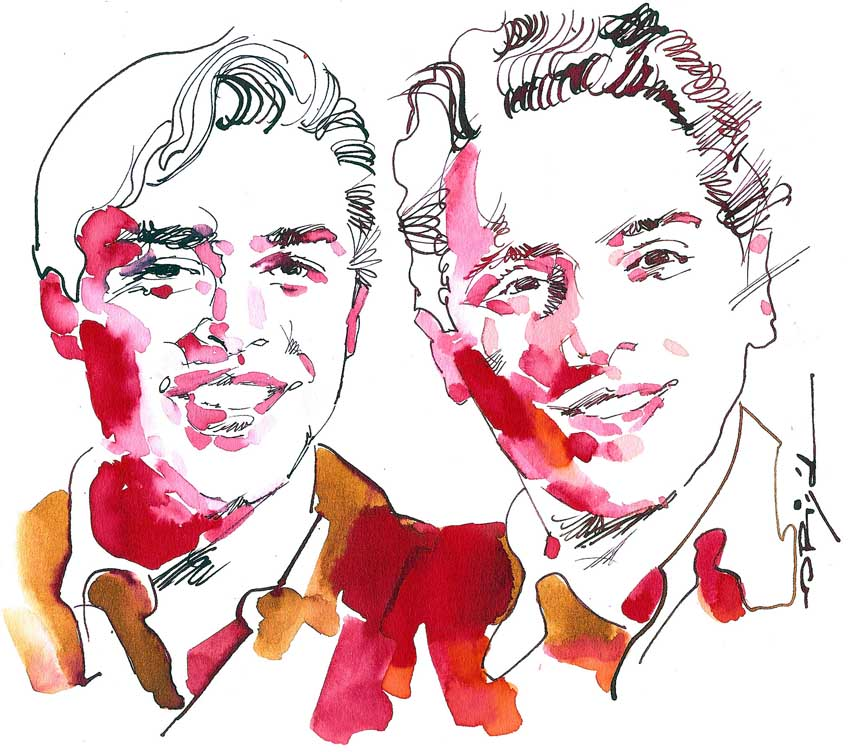
\includegraphics[width=1.0\textwidth]{Chapter5/images/PageBrin.jpg} 
        \begin{center}
        \vspace{-8pt}
    {\tiny
    \textit{image by Graziano Origa, copyright CC BY-SA 3.0}
    }
    \end{center}
\end{center}


\end{column}
\end{columns}
    

\end{frame}


\frame{\frametitle{Summary}

    \SummaryLine \vspace{4pt}
    \begin{itemize}\setlength{\itemsep}{8pt}

    \item constructing a transition matrix and a Markov Chain for a given web to model web traffic and compute the PageRank of the web
    
    \item numerical approaches to computing PageRank
    
    \end{itemize}
    
    \vspace{8pt}
    \pause 
}


% \begin{frame}
% \frametitle{Example 2 (if time permits)}



%     Construct the Google Matrix for the web below. Which page do you think will have the highest PageRank? How would your result depend on the damping factor $p$? Use software to explore these questions.     
%         \begin{center}
%         \begin{tikzpicture}
%             \begin{scope}[->,>=stealth',shorten >=1pt,auto,node distance=1.5cm,thick, main node/.style={circle,fill=black!05,draw}]
%             \node[main node] (1) {A};
%             \node[main node] (2) [right of=1] {B};
%             \node[main node] (3) [below of=1] {C};
%             \node[main node] (4) [below of=2] {D};
%             \path[every node/.style={font=\sffamily\small}]
%             (1) edge node [above] {} (3)
%             (3) edge node [above] {} (4)
%             (2) edge node [above] {} (3);
%             \end{scope}
%         \end{tikzpicture}  
%     \end{center}    

% \end{frame}

    
% \fi


%%%%%%%%%%%
% MODULE 4
% \ifnum \Week = 10
    % \newcommand{\SubTitleName}{Orthogonality} 
    % \title{Dot Products and Length}
\subtitle{\SubTitleName}
\institute[]{\Course}
\author{\Instructor}
\maketitle   
  


\tikzstyle{row} =[rectangle, minimum width=2cm, minimum height=2cm, text centered, fill=red!30,draw=green, rotate=45]

\tikzstyle{col} = [rectangle, minimum width=2cm, minimum height=2cm, text centered, fill=red!30,draw=green, rotate=135]

\tikzstyle{nul} = [trapezium, trapezium left angle=90, trapezium right angle=90, minimum width=1cm, minimum height=1cm, text centered, rotate=140]

\tikzstyle{left} = [trapezium, trapezium left angle=90, trapezium right angle=90, minimum width=1cm, minimum height=1cm, text centered, rotate=30]

\tikzstyle{arrow} = [thick,->,>=stealth]




\frame{\frametitle{Topics and Objectives}
\Emph{Topics} \\
%\TopicStatement
\begin{itemize}

    \item dot products

    \item magnitude of vectors
    
    \item distances in $\mathbb R^n$ 
    
    \item angles between vectors

    % \item Orthogonal vectors and complements
    

\end{itemize}

\vspace{0.5cm}

\Emph{Learning Objectives}\\

\LearningObjectiveStatement

\begin{itemize}

    \item characterize relationships between vectors using the (a) dot product of two vectors, (b) length (or magnitude) of a vector, (c) distance between points in $ \mathbb R^n$, and (d) angles between vectors
    
    % \item Apply theorems related to orthogonal complements, and their relationships to Row and Null space, to characterize vectors and linear systems.
\end{itemize}

} 




\begin{frame}\frametitle{The Dot Product} 

    The dot product between two vectors, $\vec u$ and $\vec v$ in $\mathbb R^n$, is defined as
    \pause 
    \vspace{-4pt}
    \begin{equation*}
    \vec u \cdot \vec v = \vec u \, ^T \vec v = 
    \begin{pmatrix*}[r]
    u_1 & u_2 & \cdots & u_n 
    \end{pmatrix*} 
    \begin{pmatrix*}[r]
    v_1 \\ v_2 \\ \vdots \\ v_n
    \end{pmatrix*} = u_1 v_1 + u_2 v_2 + \cdots + u_n v_n . 
    \end{equation*}
    
    \pause 
    
    \Emph{Example:} For what values of $k$ is $ \vec u \cdot \vec v=0$?
    
    $$\vec u = \spalignmat{ -1 ;  k; 2}, \qquad \vec v = \spalignmat{4 ;1; 3}$$

\end{frame}




\begin{frame} \frametitle{Theorem: Dot Product Identities}

    % The dot product is a special form of matrix multiplication, so it inherits its properties.  

    % \begin{center}\begin{tikzpicture} \node [mybox](box){\begin{minipage}{0.95\textwidth}
    % \vspace{4pt}
        Let $ \vec u, \vec v, \vec w$ be three vectors in $ \mathbb R ^{n}$, and $c \in \mathbb R$. 
        \begin{align*}
            \onslide<2->{(\vec v + \vec w) \cdot \vec u & = \vec v \cdot \vec u + \vec w \cdot \vec u && linearity } \\ 
            \onslide<3->{(c \vec u) \cdot \vec w &= c (\vec u \cdot \vec w) && scalars } \\ 
            \onslide<4->{\vec u \cdot \vec w &= \vec w \cdot \vec u  &&  symmetry } \\
            \onslide<5->{\vec u \cdot \vec u & \geq  \, 0 && positivity  } \\
            \onslide<6->{\vec u \cdot \vec u &= 0 \Leftrightarrow \vec u = \vec 0}
        \end{align*}

    % \end{minipage}};
    % \node[fancytitle, right=10pt] at (box.north west) {};
    % \end{tikzpicture}\end{center}



\end{frame}



\begin{frame}\frametitle{The Length of a Vector}

    % ~~ ~~ Highlight Box ~~ ~~
    \begin{center}\begin{tikzpicture} \node [mybox](box){\begin{minipage}{0.85\textwidth}\vspace{4pt}

        The \Emph{length} of a vector $\vec u \in \mathbb R^n$ is  \begin{equation*}
            \lVert \vec u\rVert = \sqrt { \vec u \cdot \vec u} = 
            \sqrt {  u_1 ^2 + u_2 ^2 + \cdots + u_n ^2 }
        \end{equation*}

    \end{minipage}};
    \node[fancytitle, right=10pt] at (box.north west) {Definition};
    \end{tikzpicture}\end{center}
    % ~~ ~~ Highlight Box ~~ ~~
    \vspace{-12pt}
    \begin{columns}
    \begin{column}{.55\textwidth}
    
    \pause 
    
    \Emph{Example} \\ If $P$ is the point $(1,3,2)$, the length of vector $\overrightarrow{OP}$ is $$\sqrt{1^2 + 3^2 + 2^2} = \sqrt{14}$$
    
    \end{column}\begin{column}{.4\textwidth}
    
        \begin{center}
        \begin{tikzpicture}[scale=0.9, axis/.style={->,black}, 
            vector/.style={-stealth,DarkBlue,very thick}, 
            vector guide/.style={dashed,gray}]
    
            \coordinate (P) at (3,2,1);
            \coordinate (O) at (0,0,0);
    
            %draw axes
            \draw[axis] (0,0,0) node[anchor=south east]{$O$} -- (4,0,0) node[anchor=north east]{$x_2$};
            \draw[axis] (0,0,0) -- (0,2.4,0) node[anchor=east]{$x_3$};
            \draw[axis] (0,0,0) -- (0,0,2) node[anchor=north]{$x_1$};
            \draw[vector] (O) -- (P) node[anchor=north west]{$P(1,3,2)$};
    
            \draw[vector guide] (3,0,1) -- (3,0,0) node[anchor=north]{$3$};
            \draw[vector guide] (3,0,1) -- (0,0,1) node[anchor=east]{$1$};
            \draw[vector guide] (3,2,1) -- (3,0,1);
            \draw[vector guide] (3,2,1) -- (0,2,1);
            \draw[vector guide] (3,2,1) -- (3,2,0);
            \draw[vector guide] (3,2,0) -- (0,2,0);
            \draw[vector guide] (0,2,0) -- (0,2,1);
            \draw[vector guide] (0,2,1) -- (0,0,1);
            \draw[vector guide] (3,2,0) -- (3,0,0);
        \end{tikzpicture}        
        \end{center}
    
    
    \end{column}
    \end{columns}

    



    




\end{frame}
 


\begin{frame} \frametitle{Example}

    Let $ \vec u, \vec v$ be two vectors in $ \mathbb R ^{n}$ with $ \lVert \vec u\rVert=5 $, $ \lVert \vec v\rVert=\sqrt 3$, and $ \vec u \cdot \vec v = - 1$. Compute the value of $ \lVert \vec u + \vec v\rVert$.  

\end{frame}





\begin{frame}\frametitle{Length of Vectors and Unit Vectors}

    \Emph{Note}: for any vector $ \vec v$ and scalar $c$, the length of $ c \vec v$ is %$ \lVert c\vec v\rVert= \lvert  c\rvert \cdot \lVert \vec v\rVert $.  
    \begin{equation*}
        \lVert c\vec v\rVert = |c| \, ||\vec v||
    \end{equation*}
    
    % ~~ ~~ Highlight Box ~~ ~~
    \begin{center}\begin{tikzpicture} \node [mybox](box){\begin{minipage}{0.85\textwidth}\vspace{2pt}

        If $ \vec v \in \mathbb R^n$ has length one, we say that it is a \Emph{unit vector.} 

    \end{minipage}};
    \node[fancytitle, right=10pt] at (box.north west) {Definition};
    \end{tikzpicture}\end{center}
    % ~~ ~~ Highlight Box ~~ ~~
    

    \vspace{6pt}
    
    \pause

    For example, each of the following vectors are unit vectors.  
    \begin{align*}
        \vec e_1 = \spalignmat{1;0} , \quad
        \vec y = \frac{1}{\sqrt 5}\spalignmat{1;2} , \quad 
        \vec v = \frac{1}{\sqrt 3}\spalignmat{1;0;1;1}
    \end{align*}

\end{frame}
 
 
 
 
 
 
 
\begin{frame}\frametitle{Distance in $ \mathbb R ^{n}$} 

    % ~~ ~~ Highlight Box ~~ ~~
    \begin{center}\begin{tikzpicture} \node [mybox](box){\begin{minipage}{0.8\textwidth}\vspace{2pt}

        For $ \vec u, \vec v \in \mathbb R ^{n}$, the \Emph{distance} between $ \vec u$ and $ \vec v$ is given by the formula $||\vec u - \vec v ||$. 

    \end{minipage}};
    \node[fancytitle, right=10pt] at (box.north west) {Definition};
    \end{tikzpicture}\end{center}
    % ~~ ~~ Highlight Box ~~ ~~
    
    \pause
    
    \Emph{Example:}
    Compute the distance from $ \vec u = \spalignmat{7;1}$ and $ \vec v = \spalignmat{3;2}$. 
    \begin{center}
        \begin{tikzpicture}[yscale=.7,xscale=.8] 
            \draw[gray](-1,-1) grid (8,3);  
            \draw[->,thick]  (-1,0) -- (8,0); 
            \draw[->,thick]  (0,-1) -- (0,3); 
            \draw[->,black,very thick] (0,0) -- (7,1) node[right] {$ \vec u$}; 
            \draw[->,black,very thick] (0,0) -- (3,2) node[above] {$ \vec v$}; 
        \end{tikzpicture}
    \end{center} 


\end{frame}


\begin{frame}\frametitle{Angles}
    
    \begin{center}
    \begin{tikzpicture} \node [mybox](box){\begin{minipage}{0.65\textwidth}
        \vspace{2pt}
        
        $ \vec a \cdot \vec b= ||\vec a|| \, ||\vec b|| \,  \cos\theta$. Thus, if $\vec a \cdot \vec b = 0$, then: 
        \begin{itemize} \setlength\itemsep{0.25em}
            \item<2-> $ \vec a$ and/or $ \vec b$ are zero vectors, or 
            \item<3-> $ \vec a$ are $ \vec b$ are perpendicular to each other. % orthogonal 
        \end{itemize}

        \end{minipage}};\node[fancytitle, right=10pt] at (box.north west) {Theorem};
    \end{tikzpicture}
    \end{center}

    \onslide<4->{
    For example, consider the vectors below.
    
     \begin{center}
        \begin{tikzpicture}[scale=0.5] 
            \draw[->,DarkBlue,very thick,-stealth] (0,0) -- (9,1) node[right] {$ \vec b$}; 
            \draw[->,DarkRed,very thick,-stealth] (0,0) -- (3,3) node[above] {$ \vec a$}; 
            \draw[->,DarkGreen,very thick,-stealth] (0,0) -- (-3/9,3) node[above] {$ \vec c$}; 
            % \draw[DarkRed] (2,2/9) arc (0:58:1.3) node[midway, right] {$\theta$};            
            \draw[DarkGreen] (1.5,0.1666) arc (0:110:1.2) node[midway, above] {$\frac{\pi}{2}$};            
        \end{tikzpicture}
    \end{center} 
    }
    
\end{frame}



\frame{\frametitle{Summary}

    \SummaryLine \vspace{4pt}
    \begin{itemize}\setlength{\itemsep}{8pt}

    \item dot products

    \item magnitude of vectors
    
    \item distances in $\mathbb R^n$ 
    
    \item angles between vectors
    
    \end{itemize}
    
    \vspace{8pt}
    
}


 % done
    % \title{Orthogonality}
\subtitle{\SubTitleName}
\institute[]{\Course}
\author{\Instructor}
\maketitle   
  

\frame{\frametitle{Topics and Objectives}
\Emph{Topics} \\
%\TopicStatement
\begin{itemize}

    % \item dot products

    % \item magnitude of vectors
    
    % \item distances in $\mathbb R^n$ 
    
    % \item angles between vectors

    \item orthogonal vectors and dot products
    
    % \item orthogonal compliments
    

\end{itemize}

\vspace{0.5cm}

\Emph{Learning Objectives}\\

\LearningObjectiveStatement

\begin{itemize}

    % \item characterize relationships between vectors using the (a) dot product of two vectors, (b) length (or magnitude) of a vector, (c) distance between points in $ \mathbb R^n$, and (d) angles between vectors
    
    \item apply theorems related to orthogonality to characterize vectors
    
\end{itemize}

} 



\begin{frame}\frametitle{Orthogonality}

    \begin{center}\begin{tikzpicture} \node [mybox](box){\begin{minipage}{0.75\textwidth} \vspace{4pt}
    Two vectors $ \vec u$ and $ \vec v$ are \Emph{orthogonal} if $ \vec u \cdot \vec v =0$.  
    This is equivalent to: 
    \begin{equation*}
    \lVert \vec u + \vec v \rVert ^2 =  \lVert \vec u  \lVert^2  +  \lVert  \vec v \rVert ^2
    \end{equation*}
    \end{minipage}};
    \node[fancytitle, right=10pt] at (box.north west) {Definition (Orthogonal Vectors)};
    \end{tikzpicture}\end{center}

    \onslide<2->{This is because:} 
    \begin{align*}
        \onslide<3->{||\vec u + \vec v||^2 &= (\vec u + \vec v) \cdot (\vec u + \vec v) \\ &= } 
        \onslide<4->{  \vec u \cdot \vec u + \vec v \cdot \vec v + 2 \vec u \cdot \vec v \\}
        \onslide<5->{&= \lVert \vec u  \lVert^2  +  \lVert  \vec v \rVert ^2 + 2 \vec u \cdot \vec v}
    \end{align*}
    \onslide<6->{But if $\vec u$ and $\vec v$ are orthogonal, $\vec u \cdot \vec v = 0$.}

\end{frame}


\begin{frame}\frametitle{Orthogonality and the Pythagorean Theorem}

    If $ \vec u$ and $ \vec v$ are vectors in $\mathbb R^n$, the expression 
    
    $$\lVert \vec u + \vec v \rVert ^2 =  \lVert \vec u  \lVert^2  +  \lVert  \vec v \rVert ^2$$ 
    
    \vspace{12pt}
    is an $n$-dimensional version of the Pythagorean Theorem.

    \vspace{12pt}
    
    \onslide<2->{\Emph{Example}: if $\vec u = \spalignmat{1;1}$ and $\vec v = \spalignmat{1;-1}$, then $\vec u \cdot \vec v = 0$, and }
    \begin{align*}
        \onslide<3->{\lVert \vec u + \vec v \rVert^2 = \left\lVert \spalignmat{2;0} \right\rVert^2 &= \left(\sqrt{2^2 + 0^2 }\right)^2 = 4 } \\
        \onslide<4->{\lVert \vec u \rVert ^2 + \lVert \vec v \rVert^2 &= 2 + 2 = 4 } 
    \end{align*}    
    \onslide<5->{The 2-dimensional Pythagorean Theorem is satisfied. }
\end{frame}









\begin{frame}\frametitle{Orthogonality and the Zero Vector}

        \begin{itemize}\setlength{\itemsep}{8pt}
        \item<1-> The zero vector in $\mathbb R^n$ is orthogonal to every vector in $\mathbb R^n$. 
        \item<2-> We usually only mean non-zero vectors when discussing orthogonality.
    \end{itemize} 
    
\end{frame}









\begin{frame}\frametitle{Example}

    Sketch the set of all vectors that are orthogonal to $ \vec v = \spalignmat{3;2}$. Is our set also a subspace? \pause 
    \begin{center}
    \begin{tikzpicture}[yscale=.5,xscale=.5] 
        \draw[gray](-4,-4) grid (4,4);  
        \draw[->,very thick]  (-4,0) -- (4,0) node[above]{$x_1$}; 
        \draw[->,very thick]  (0,-4) -- (0,4) node[above]{$x_2$}; 
        \draw[->,DarkBlue,very thick] (0,0) -- (3,2) node[above] {$ \vec v$}; 
    \end{tikzpicture}
    \end{center} 
\end{frame} 


\frame{\frametitle{Summary}

    \SummaryLine \vspace{4pt}
    \begin{itemize}\setlength{\itemsep}{8pt}

        \item orthogonal vectors and dot products
        \item orthogonal vectors and the Pythagorean Theorem
        \item sketching the set of vectors that are orthogonal to a given vector in $\mathbb R^2$
    
    \end{itemize}
    
    \vspace{8pt}
    \onslide<2->{A key concept in this video was that if $ \vec u$ and $ \vec v$ are \Emph{orthogonal}, then $ \vec u \cdot \vec v =0$, and 
    \begin{equation*}
    \lVert \vec u + \vec v \rVert ^2 =  \lVert \vec u  \lVert^2  +  \lVert  \vec v \rVert ^2
    \end{equation*}
    \vspace{12pt}
    This is an $n$-dimensional version of the Pythagorean Theorem. 
    }
}




 % done
    % \title{Orthogonal Compliments}
\subtitle{\SubTitleName}
\institute[]{\Course}
\author{\Instructor}
\maketitle   
  


\frame{\frametitle{Topics and Objectives}
\Emph{Topics} \\
%\TopicStatement
\begin{itemize}

    % \item dot products

    % \item magnitude of vectors
    
    % \item distances in $\mathbb R^n$ 
    
    % \item angles between vectors

    % \item orthogonal vectors and dot products
    
    \item orthogonal compliments
    

\end{itemize}

\vspace{0.5cm}

\Emph{Learning Objectives}\\

\LearningObjectiveStatement

\begin{itemize}

    % \item characterize relationships between vectors using the (a) dot product of two vectors, (b) length (or magnitude) of a vector, (c) distance between points in $ \mathbb R^n$, and (d) angles between vectors
    
    \item apply theorems related to orthogonality to characterize vectors and subspaces
    
\end{itemize}

} 




\begin{frame}[t]\frametitle{Orthogonal Compliments} 

\vspace{-10pt} 

\begin{center}\begin{tikzpicture} \node [mybox](box){\begin{minipage}{0.95\textwidth}

\vspace{2pt} 

    Let $W$ be a subspace of $\mathbb R ^{n}$.  Vector $\vec z \in \mathbb R ^{n}$ is \Emph{orthogonal} to $W$ if $\vec z$ is orthogonal to every vector in $W$.

    \vspace{12pt} 

    The set of all vectors orthogonal to $ W$ is a subspace, the \Emph{orthogonal compliment} of $W$, or $ W ^{\perp}$.
    \begin{equation*}
        W ^{\perp} = \{ \vec z \in \mathbb R ^{n}  \;:\;  \vec z \cdot  \vec w = 0 \ \text{for all } \vec w \in W \} 
    \end{equation*}

\end{minipage}};
\node[fancytitle, right=10pt] at (box.north west) {Definitions};
\end{tikzpicture}\end{center}

\end{frame}









\begin{frame}\frametitle{Example: $(\text{Col} A)^{\perp}$} 


\begin{columns}
\begin{column}{0.5\textwidth}
   Suppose $A = \spalignmat{1 3;2 6}$. 
   \begin{itemize}
       \item<2-> $\text{Col} A$ is the span of $\vec a_1 = \spalignmat{1;2}$  
       \item<3-> $(\text{Col} A )^{\perp}$ is the span of $\vec z = \spalignmat{2;-1}$
   \end{itemize}\end{column}\begin{column}{0.5\textwidth}  \vspace{-1cm} \begin{center}\begin{tikzpicture}
   [scale=.6,
   vectorblue/.style={-stealth,DarkBlue,very thick},
   vectorred/.style={-stealth,DarkRed,very thick}]
   \onslide<4->{
        \draw[help lines] (-4, -4) grid (4, 4);
        \draw[thick, ->] (-4, 0) -- (4, 0) node[anchor=west] {$x_1$};
        \draw[thick, ->] (0, -4) -- (0, 4) node[anchor=south] {$x_2$};
    }
    \onslide<5->{
        \draw[vectorblue]   (0,0) -- (1,2) node[anchor=west]{$\vec a_1$};
    }
    \onslide<6->{
        \node[overlay, above] at (3, 3) {Col$A$};
        \draw[-] (-2,-4) -- (2,4);
    }
    \onslide<7->{
        \draw[vectorred]   (0,0) -- (2,-1) node[anchor= north]{$\vec z$};
    }
    \onslide<8->{
        \node[overlay, below] at (3, -2) {$(\Col A)\Perp$};
        \draw[-] (-4,2) -- (4,-2);
        \draw[vectorred]   (0,0) -- (2,-1) node[anchor= north]{$\vec z$};
    }    
    \end{tikzpicture}
    \end{center}
\end{column}
\end{columns}


\end{frame}



\begin{frame}\frametitle{Example: $(\text{Nul} A)^{\perp}$} 

For $A = \spalignmat{1 3;2 6}$, sketch Nul$A$ and (Nul$A)^{\perp}$ on the grid below. 

\begin{center}
\begin{tikzpicture}
   [scale=.6,
   vectorblue/.style={-stealth,DarkBlue,very thick},
   vectorred/.style={-stealth,DarkRed,very thick}]
    \draw[help lines] (-4, -4) grid (4, 4);
    \draw[thick, ->] (-4, 0) -- (4, 0) node[anchor=west] {$x_1$};
    \draw[thick, ->] (0, -4) -- (0, 4) node[anchor=south] {$x_2$};
    \end{tikzpicture}
    \end{center}

\end{frame}









\begin{frame}\frametitle{Example: Equation of a Plane} 

    Line $L$ is a subspace of $\R^3$ spanned by $\vec v = \spalignmat{1;-1;2}$. Then the space $ L^{\perp}$ is a plane. Construct an equation of the plane $ L ^{\perp}$. 
    
    \vspace{6pt}

    \tdplotsetmaincoords{80}{100}
        \begin{tikzpicture}[
        scale=1.4,
        tdplot_main_coords,
        line/.style={DarkRed},
        vector/.style={-stealth,DarkBlue,very thick},
        vector guide/.style={dashed,gray}
        ]
        
            \coordinate (P) at (2,-1,2);  
            \coordinate (Q) at (2.4,-1.2,2.4);
            \coordinate (R) at (-1.2,.6,-1.2);
            \coordinate (O) at (0,0,0);
            
            % Draw Axes
            \draw[thick,->] (O) -- (2.8,0,0) node[anchor=north east]{$x$};
            \draw[thick,->] (0,-2,0) -- (0,2,0) node[anchor=north west]{$y$};
            \draw[thick,->] (O) -- (0,0,2) node[anchor=south]{$z$};            
            
            % Draw Plane (assume instructor will annotate slide with OneNote)
%            \filldraw[
%                draw=DarkBlue,% color of edge
%                fill=DarkBlue!20,% color of fill
%                opacity=.6, % sets opacity of fill and of edges
%            ]          
%            (-1,-1,0)
%            -- (1,1,0)
%            -- (-1,1,0)
%            -- (-3,-1,0)            
%            -- cycle;
  
            % Draw Vector and Line L
            \draw[line]     (R) -- (Q) node[anchor=north east]{$L$};
            \draw[vector]   (O) -- (P) node[anchor=north east]{$\vec v$};

            % Draw vector guides
            \draw[vector guide] (2,-1,0) -- (2,0,0) node[anchor= west]{$1$};      
            \draw[vector guide] (2,-1,0) -- (0,-1,0) node[anchor=south west]{$-1$};      
            \draw[vector guide] (2,-1,0) -- (2,-1,2);      
            
        \end{tikzpicture}
    
    % \begin{center} {\small Can also visualise line and plane with CalcPlot3D: \underline{web.monroecc.edu/calcNSF}} \end{center}

\end{frame}













    
    
    
\frame{\frametitle{Summary}

    \SummaryLine \vspace{4pt}
    \begin{itemize}\setlength{\itemsep}{8pt}

        \item orthogonal vectors and dot products
        
        \item orthogonal compliments
        
    \end{itemize}
    
    \vspace{8pt}
    \onslide<2->{A key concept in this video was that if $W$ is a subspace of $\mathbb R^n$, the \Emph{orthogonal compliment} of that subspace, or $W\Perp$, is the set of all vectors orthogonal to the vectors in $W$. }
}


 % done 
    % 
\title{The Four Fundamental Subspaces}
\subtitle{\SubTitleName}
\institute[]{\Course}
\author{\Instructor}
\maketitle   
  

\frame{\frametitle{Topics and Objectives}
\Emph{Topics} \\
%\TopicStatement
\begin{itemize}

    % \item dot products

    % \item magnitude of vectors
    
    % \item distances in $\mathbb R^n$ 
    
    % \item angles between vectors

    \item relationships between $\Row A$, $\Col A$, $\Nul A$, and $\Nul A^T$
    

\end{itemize}

\vspace{0.5cm}

\Emph{Learning Objectives}\\

\LearningObjectiveStatement

\begin{itemize}

    \item construct a basis for the four fundamental subspaces of a rectangular matrix
    
\end{itemize}

} 


\begin{frame}\frametitle{Row$A$}
    
    \begin{center}
    \begin{tikzpicture} \node [mybox](box){\begin{minipage}{0.75\textwidth}
        \vspace{2pt}
        
        Row$A$ is the space spanned by the rows of matrix $A$.

        \end{minipage}};\node[fancytitle, right=10pt] at (box.north west) {Definition};
    \end{tikzpicture}
    \end{center}

	We can show that
	\vspace{6pt}
	\begin{itemize} \setlength\itemsep{1em}
		\item<2-> a basis for Row$A$ is given by the pivot rows of $A$
		\item<3-> $\dim(\Row A) = \dim(\Col A)$
	    \item<4-> $\Row A = \Col A^T$
	    \item<5-> in general $\Row A$ and $\Col A$ are not related to each other
	\end{itemize}

\end{frame}









\begin{frame}{Revisiting the Rank Theorem}

    Recall from earlier in the course, that if $N$ is the number of columns in a matrix, that
    
    $$N = \dim (\Col A) + \dim (\Nul A)$$
    \vspace{2pt}
    \pause
    
    But if dim(Row $A$) = dim(Col $A$), then we could express this as
    
    $$N = \dim (\Row A) + \dim (\Nul A)$$
    \vspace{2pt}
    \pause
    
    In fact, there are many other equivalent ways of expressing the above theorem. 
    
\end{frame}



\begin{frame} \frametitle{Relationships Between $\Row A$ and $\Nul A$} 

    % Describe the Null$(A)$ in terms of an orthogonal subspace.  \\[12pt]
    
    Suppose vector $ \vec v$ is in $ \Null A$.
    
    \vspace{4pt}

    \begin{itemize}  \setlength\itemsep{1em}
    
        \item<1-> then $ A \vec v =  \vec 0$
        
        \item<2-> we compute $A\vec v$ by taking dot products between each row of $A$ and $\vec v$
        
        \item<3-> all of these dot products are zero, so $ \vec v$ is orthogonal to the rows of $A$

        \item<4-> therefore, $\Row A  $ is  orthogonal to $\Null A $
        
        \item<5-> in other words, $(\Row A)\Perp = \Null A$

    \end{itemize}
    
    \vspace{4pt}
    \onslide<6->{Or, we could also say that $\Row A = (\Null A)\Perp$. }
    
\end{frame}


\begin{frame} \frametitle{Relationships Between Col$A$ and Nul$A^T$} 

    There is a similar relationship between $\Col A$ and $\Nul A^T$. Suppose vector $ \vec x$ is in $ \Null A^T$.

    \begin{itemize}  \setlength\itemsep{1em}
        \item<1-> then $ A^T \vec x =  \vec 0$
        
        \item<2-> this implies that $ \vec x$ is orthogonal to the rows of $ A^T$

        \item<3-> this implies that $ \vec x$ is orthogonal to the columns of $ A$

        \item<4-> therefore, $\Col A  $ is  orthogonal to $\Null A^T $
        
        \item<5-> in other words, $(\Col A)\Perp = \Nul A^T$

    \end{itemize}
    
    
\end{frame}




\begin{frame}{The Four Fundamental Subspaces}

    \begin{center}\begin{tikzpicture} \node [mybox](box){\begin{minipage}{0.85\textwidth}\vspace{2pt}
    For any $ A \in \mathbb R^{m\times n}$,  the orthogonal complement of $\Row A$ is $ \Null A$, and the orthogonal complement of $ \Col A$ is  $ \Null A ^{T}$.  

    \end{minipage}};
    \node[fancytitle, right=10pt] at (box.north west) {Theorem (The Four Subspaces)};
    \end{tikzpicture}\end{center}

    % The idea behind this theorem is described in the diagram below. 
    \pause 
    
    \begin{center}
    \begin{tikzpicture}[scale=.85]
        

        
        \onslide<2->{
        % boxes
        \filldraw[draw=DarkBlue!50,fill=DarkBlue!15] (0,0) -- (-1,1) -- (1,3) -- (2,2) -- cycle;
        \filldraw[draw=DarkBlue!50,fill=DarkBlue!15] (0,0) -- (1,-1) -- (0,-2) -- (-1,-1) -- cycle;      
        \draw (0.4, 1.7) node[below]{\small $\Row A$};
        \draw (0.0,-0.7) node[below]{\small $\Nul A$};        
        }
        
        \onslide<3->
        {
        \filldraw[draw=DarkGreen!50,fill=DarkGreen!15] (4,0) -- (2.5, 1.5) -- (3.5, 2.5) -- (5,1) -- cycle;
        \filldraw[draw=DarkGreen!50,fill=DarkGreen!15] (4,0) -- (5.5,-1.5) -- (4.5,-2.5) -- (3,-1) -- cycle;        
        \draw (3.9, 1.5) node[below]{\small $\Col A$};
        \draw (4.2, -0.8) node[below]{\small $\Nul A^T$};        
        }

        \onslide<4->{
        \draw (-1.0,0.5) node[below]{\Large $\color{DarkBlue} \mathbb R^n$};
        }

        \onslide<5->{
        \draw ( 5.0,0.5) node[below]{\Large $\color{DarkGreen} \mathbb R^m$};
        }
        
    \end{tikzpicture}
    \end{center}

\end{frame}

\begin{frame}\frametitle{Example} 

    Suppose $A = \spalignmat{1 3 0 ; 0 0 1 ; 0 0 0 }$. Construct a basis for the following.
    \begin{enumerate} \setlength{\itemsep}{24pt}
        \item $\Row A$
        \item $(\Row A)^{\perp}$
        \item $\Col A$
        \item $(\Col A)^{\perp}$    
    \end{enumerate}

\end{frame}



\frame{\frametitle{Summary}

    \SummaryLine \vspace{4pt}
    \begin{itemize}\setlength{\itemsep}{8pt}

    \item orthogonality relationships between the four fundamental subspaces: $\Row A, \Col A, (\Row A)\Perp,$ and $(\Col A)\Perp$
    
    \end{itemize}
    
    \vspace{8pt}
    
}







% \begin{frame}\frametitle{Additional Example (if time permits)}
%     $A$ has the LU factorization: 
        
%         $$A=L U = \spalignmat{1 0 0;1 1 0;0 4 1} \spalignmat{1 0 2 0;0 1 -1 2;0 0 0 0}$$
        
%         \begin{itemize}[a)]
%             \item Construct a basis for $(\mathrm{Row}A)^{\perp}$
%             \item Construct a basis for $(\mathrm{Col}A)^{\perp}$
%         \end{itemize}
%         \textit{Hint: it is not necessary to compute $A$. Recall that $A^T = U^TL^T$, matrix $L^T$ is invertible, and $U^T$ has a non-trivial nullspace}. 
% \end{frame}




% \begin{frame}\frametitle{Looking Ahead - Projections}

%     Suppose we want to find the closest vector in Span$\{\vec b\}$ to $\vec a$. 
%      \begin{center}
%         \begin{tikzpicture}[scale=0.8] 
%             \draw[-,gray, dashed] (-1,-1/9) -- (11,11/9) node[below, right] {Span$\{\vec b\}$}; 
%             \draw[->,DarkBlue, thick,-stealth] (0,0) -- (9,1) node[below,right] {$ \vec b$}; 
%             \draw[->,DarkRed, thick,-stealth] (0,0) -- (3,3) node[above] {$ \vec a = \hat a + \vec w$}; 
%             \draw[->,black, very thick,-stealth] (0,0) -- (3.3,3.3/9) node[below] {$\hat a = $proj$_{\vec b} \vec a$}; 
%             \draw[->,DarkGreen,very thick, dashed, -stealth] (3.3,3.3/9) -- (3,2.8) node[below, right] {$\vec w$}; 
%             %\draw[black] (2,2/9) arc (0:100:0.85) node[midway, right] {$\theta$};            
%         \end{tikzpicture}
%     \end{center} 
    
%     \begin{itemize}
%         \item later we draw connections between dot products and \Emph{projections}
%         % \item the 
%         \item projections are also used throughout multivariable calculus courses
%     \end{itemize}    
    
% \end{frame}
 



 % done 
    % \title{Orthogonal Bases}
\subtitle{\SubTitleName}
\institute[]{\Course}
\author{\Instructor}
\maketitle   
  

 
\begin{frame}\frametitle{Topics and Objectives}
\Emph{Topics} \\
%\TopicStatement
\begin{itemize}

    \item orthogonal sets of vectors

    \item orthogonal and orthonormal bases 
    

\end{itemize}

\vspace{0.5cm}

\Emph{Learning Objectives}\\

\LearningObjectiveStatement

\begin{itemize}
    % \item compute orthogonal projections and distances
    % \item express a vector as a linear combination of orthogonal vectors
    % \item characterize bases for subspaces of $\mathbb R^n$, and
    \item determine whether a basis is orthogonal or whether it is orthonormal
    \item construct and give examples of orthogonal and orthonormal bases
\end{itemize}


\end{frame}


\begin{frame}{Orthogonal Vector Sets}

    % ~~ ~~ Highlight Box ~~ ~~
    \begin{center}\begin{tikzpicture} \node [mybox](box){\begin{minipage}{0.85\textwidth}\vspace{2pt}

        A set of vectors $ \{\vec u_1 ,\dotsc, \vec u_p\}$ are an \Emph{orthogonal set} of vectors if for each $ j\neq k$, $ \vec u_j \perp \vec u_k$.  

    \end{minipage}};
    \node[fancytitle, right=10pt] at (box.north west) {Definition};
    \end{tikzpicture}\end{center}
    % ~~ ~~ Highlight Box ~~ ~~
        
    \vspace{4pt} 
    \pause 
    
    \Emph{Example:} Fill in the missing entries to make $ \{\vec u_1 ,\vec u_2, \vec u_3\}$ a set of non-zero orthogonal vectors.
    \begin{equation*}
        \vec u_1 = \begin{pmatrix} 4 \\ 0 \\ 1 \end{pmatrix}, \quad 
        \vec u_2 = \begin{pmatrix}-2 \\ 0 \\    \phantom{-1 - 1 }\end{pmatrix}, \quad 
        \vec u_3 = \begin{pmatrix} 0 \\  \phantom{-1 - 1 } \\ \phantom{-1 - 1 }\end{pmatrix}
    \end{equation*}
\end{frame}


\begin{frame}{Orthogonal Vector Sets}
    \Emph{Example:} Fill in the missing entries to make $ \{\vec u_1 ,\vec u_2, \vec u_3\}$ a set of non-zero orthogonal vectors.
    \begin{equation*}
        \vec u_1 = \begin{pmatrix} 4 \\ 0 \\ 1 \end{pmatrix}, \quad 
        \vec u_2 = \begin{pmatrix}-2 \\ 0 \\    \phantom{-1 - 1 }\end{pmatrix}, \quad 
        \vec u_3 = \begin{pmatrix} 0 \\  \phantom{-1 - 1 } \\ \phantom{-1 - 1 }\end{pmatrix}
    \end{equation*}
    
    \Emph{Solution}\\ \pause
    We need $\vec u_1\cdot \vec u_2 = 0$\pause, so we need $\vec u_2 = \begin{pmatrix} -2\\0 \\ 8 \end{pmatrix}$. 
    
    \pause 
    
    \vspace{12pt}
    
    We also need $\vec u_3\cdot \vec u_1 = \vec u_3 \cdot \vec u_2 = 0$, so we can set $\vec u_3 = \begin{pmatrix} 0 \\ 1 \\ 0 \end{pmatrix}$.

\end{frame}



\begin{frame}{Orthogonality and Linear Independence}
\begin{center}\begin{tikzpicture} \node [mybox](box){\begin{minipage}{0.85\textwidth} \vspace{4pt}
    Let  $S = \{\vec u_1 ,\dotsc, \vec u_p\}$ be an \Emph{orthogonal set} of vectors.  %Then, for scalars $ c_1 ,\dotsc, c_p$, 
    % \begin{equation*}
    % \bigl\lVert c_1 \vec u_1 + \cdots + c_p \vec u_p  \bigr\rVert ^2 
    % = c_1 ^2 \lVert \vec u_1 \rVert ^2 + \cdots + c_p ^2 \lVert \vec u_p\rVert ^2 . 
    % \end{equation*}    In particular, 
    If $ \vec u_i$ are non-zero, the then $S$ is a set of \Emph{linearly independent} vectors. 
    \end{minipage}};
    \node[fancytitle, right=10pt] at (box.north west) {Theorem};
    \end{tikzpicture}\end{center}
    \vspace{6pt}
    \pause
    \Emph{Proof}: Suppose $ \{\vec u_1 ,\dotsc, \vec u_p\}$ are a set of non-zero orthogonal vectors, \pause and $$\sum_{i=1}^ p c_i\vec u_i = c_1 \vec u_1 + c_2 \vec u_2  + \ldots + c_p \vec u_p = \vec 0$$ for scalars $c_1, c_2, \ldots , c_p$, then $\ldots$

\end{frame}


\begin{frame}{Orthogonality and Linear Independence}

    Then 
    \begin{align*}
        0 &= \vec u_1 \cdot \vec 0 \\
        \onslide<2->{&= \vec u_1 \cdot \sum_{i=1}^ p c_i\vec u_i} \\
        \onslide<3->{&= \sum_{i=1}^ p c_i \vec u_1 \cdot \vec u_i} \\
        \onslide<4->{&= c_1 \vec u_1 \cdot \vec u_1} 
    \end{align*}
    \onslide<5->{But $\vec u_1$ is not the zero vector, so $c_1=0$. Likewise, $c_2, c_3 , \ldots c_p$ must also be zero, which means that $S$ is a set of linearly independent vectors.  }
\end{frame}





\begin{frame}{Orthogonal Bases}

    \vspace{-12pt}
    
    \begin{center}\begin{tikzpicture} \node [mybox](box){\begin{minipage}{0.85\textwidth}\vspace{4pt}
        Let  $ \{\vec u_1 ,\dotsc, \vec u_p\}$ be an orthogonal  basis for a subspace $ W$ of $ \mathbb R ^{n}$. Then, for any vector $ \vec w\in W$, 
        \begin{equation*}
            \vec w= c_1  \vec u_1   + \cdots + c_p   \vec u_p  . 
        \end{equation*}
        Above, the scalars are $ \displaystyle c_ q = \frac { \vec w \, \cdot \, \vec u_q } { \vec u _{q} \cdot \, \vec u_q }$. 
    \end{minipage}};
    \node[fancytitle, right=10pt] at (box.north west) {Theorem (Expansion in Orthogonal Basis) };
    \end{tikzpicture}\end{center}
    \pause
    Obtaining the coefficients, $ \displaystyle c_ q$, with the above formula is generally more efficient than row reduction.  \pause However, we can only apply this theorem when we have an orthogonal basis for $W$. 
\end{frame}










\begin{frame}{Example: Orthogonal Basis}  
    \vspace{-6pt}
    Suppose $W$ is the subspace of $\mathbb R ^{3}$ that is orthogonal to $\vec x$. 
    $$\vec x = \spalignmat{1;1;1}, \quad \vec u = \spalignmat{1;-2;1}, \quad \vec v = \spalignmat{-1;0;1}, \quad \vec s = \spalignmat{3;-4;1}$$
    \begin{enumerate}
        \item Confirm that an orthogonal basis for $W$ is given by $\vec u$ and $\vec v$.
        \item Assume $\vec s \in W$. Compute the expansion of $\vec s$ in the basis for $W$.
    \end{enumerate}
\end{frame}


\begin{frame}{Solution to Part 1}  
    \vspace{-6pt}
    Suppose $W$ is the subspace of $\mathbb R ^{3}$ that is orthogonal to $\vec x$. 
    $$\vec x = \spalignmat{1;1;1}, \quad \vec u = \spalignmat{1;-2;1}, \quad \vec v = \spalignmat{-1;0;1}, \quad \vec s = \spalignmat{3;-4;1}$$ \vspace{-12pt}
    \begin{enumerate}
        \item Confirm that an orthogonal basis for $W$ is given by $\vec u$ and $\vec v$.
        % \item Assume $\vec s \in W$. Compute the expansion of $\vec s$ in the basis for $W$.
    \end{enumerate}
    
    \pause 
    \Emph{Solution to Part 1}\\ \pause 
    For $\vec u$ and $\vec v$ to form an orthogonal basis for $W$, (a) $\vec u$ and $\vec v$ must be in $W$, and (b) they must be orthogonal.  \pause 
    \begin{enumerate}[a)]
        \item $\vec x \cdot \vec u = 1 -2 +1 = 0$ and $\vec x \cdot \vec v = -1 + 0 + 1 = 0 $ so $\vec u$ and $\vec v$ are in $W$. 
        \item $\vec u \cdot \vec v = -1 + 0 -1 = 0$, so $\vec u$ and $\vec v$ are orthogonal.
    \end{enumerate}
    \pause 
    Thus, $\vec u$ and $\vec v$ form an orthogonal basis for $W$. 
\end{frame}



\begin{frame}{Solution to Part 2}  
    \vspace{-6pt}
    Suppose $W$ is the subspace of $\mathbb R ^{3}$ that is orthogonal to $\vec x$. \pause 
    $$\vec x = \spalignmat{1;1;1}, \quad \vec u = \spalignmat{1;-2;1}, \quad \vec v = \spalignmat{-1;0;1}, \quad \vec s = \spalignmat{3;-4;1}$$ \vspace{-12pt} \pause 
    \begin{enumerate}
        % \item Confirm that an orthogonal basis for $W$ is given by $\vec u$ and $\vec v$.
        \item[2.] Assume $\vec s \in W$. Compute the expansion of $\vec s$ in the basis for $W$.
    \end{enumerate}
    
    \vspace{12pt}
    \Emph{Solution to Part 2}\\ \pause 
    Given that $\vec s$ is in $W$, and we have an orthogonal basis for $W$, we can use our theorem to write: \pause 
    $$\vec s = \frac{\vec s \cdot \vec u}{\vec u \cdot \vec u}\vec u + \frac{\vec s \cdot \vec v}{\vec v \cdot \vec v}\vec v=\frac{12}{6}\vec u + \frac{-2}{2}\vec v = 2\vec u - \vec v$$ \pause 
    Therefore, $\vec s = 2\vec u - \vec v$. 
\end{frame}


\begin{frame}{Definition}
    \begin{center}\begin{tikzpicture} \node [mybox](box){\begin{minipage}{0.85\textwidth}\vspace{4pt}
        An \Emph{orthonormal basis} for a subspace $ W$ is an orthogonal basis $ \{\vec u_1 ,\dotsc, \vec u_p\}$ 
        in which every vector $ \vec u_q$ has unit length.  In this case, for each $ \vec w\in W$,  
        \begin{gather*}
        \vec w = (\vec w \cdot \vec u_1) \vec u_1 + \cdots +  (\vec w \cdot \vec u_p ) \vec u_p
        \\
        \lVert \vec w \rVert  =  \sqrt{(\vec w \cdot \vec u_1) ^2 + \cdots +  (\vec w \cdot \vec u_p) ^2} 
    \end{gather*}
    \end{minipage}};
    \node[fancytitle, right=10pt] at (box.north west) {Definition  (Orthonormal Basis)};
    \end{tikzpicture}\end{center}
\end{frame}




\begin{frame}{Example: Orthonormal Basis}  
    \vspace{-6pt}
    $ W $ is a subspace of $ \mathbb R ^{3}$ that is perpendicular to $x$.  Calculate the missing coefficients in the orthonormal basis for $W$, which is $\{u, v\}$. 
    \begin{equation*}
    x = \spalignmat{1;1;1}, \qquad 
    u = 
    \frac{1}{\sqrt{\quad}}
    \begin{pmatrix}
        1 \\ 0 \\ \phantom {\int\int} 
    \end{pmatrix} ,
    \qquad 
    v= 
    \frac{1}{\sqrt{\quad}}
    \begin{pmatrix}
        \phantom {\int\int}  \\ \phantom {\int\int}  \\ \phantom {\int\int} 
    \end{pmatrix} 
    \end{equation*}
    \Emph{Solution for $u$}\\    
    \pause For $u$ to be in $W$ we need $x\cdot u =0$. \pause 
    $$\text{Set } u=\frac{1}{\sqrt a}\begin{pmatrix} 1\\0\\b \end{pmatrix} \quad \Rightarrow \quad \pause x\cdot u = \frac{1}{\sqrt{a}}(1+0+b)=0 \quad \Rightarrow \quad b = -1$$
    \pause For $u$ to have unit length, we need $a=2$. 
\end{frame}



\begin{frame}{Example: Orthonormal Basis}  
    \vspace{-12pt}
    % $ W $ is a subspace of $ \mathbb R ^{3}$ that is perpendicular to $x$.  Calculate the missing coefficients in the orthonormal basis for $W$, which is $\{u, v\}$. 
    \begin{equation*}
    x = \spalignmat{1;1;1}, \qquad 
    u = 
    \frac{1}{\sqrt{2}}
    \begin{pmatrix}
        1 \\ 0 \\ -1
    \end{pmatrix} ,
    \qquad 
    v= 
    \frac{1}{\sqrt{\quad}}
    \begin{pmatrix}
        \phantom {\int\int}  \\ \phantom {\int\int}  \\ \phantom {\int\int} 
    \end{pmatrix} 
    \end{equation*}
    \pause 
    \Emph{Solution for $v$}\\
    For $u$ and $v$ to form an orthonormal basis, we need $u\cdot v=0$. \pause $$ \text{Set } v=\frac{1}{\sqrt k}\begin{pmatrix} c_1\\c_2\\c_3 \end{pmatrix} \quad \Rightarrow u\cdot v \text{ implies } c_1=c_3$$ If $v$ is in $W$ we need $x\cdot v =0$. \pause 
    $$x\cdot v = \frac{1}{\sqrt{k}}(c_1+c_2+c_3)=0 \quad \Rightarrow \quad c_2 = -2c_1$$
    \pause Choosing $c_1 = 1$, then $c_2 = -2$ and $c_3=1$. \pause For $\|v\| = 1$, we need $k=6$. 
\end{frame}


\begin{frame}{Example: Orthonormal Basis}  
    Our vectors are:
    \begin{equation*}
    x = \spalignmat{1;1;1}, \qquad 
    u = 
    \frac{1}{\sqrt{2}}
    \begin{pmatrix}
        1 \\ 0 \\ -1
    \end{pmatrix} ,
    \qquad 
    v= 
    \frac{1}{\sqrt{6}}
    \begin{pmatrix}
        1 \\-2\\1
    \end{pmatrix} 
    \end{equation*}
    \pause As required, $u$ and $v$ are orthonormal, \pause and they form a basis for $W$, which is the set of vectors orthogonal to $x$. 
\end{frame}



\begin{frame}{Orthogonal Bases}

    Do not forget that bases are not unique. 
    
    \vspace{12pt} 
    
    \pause 
    
    For example, any vector $\vec w \in \mathbb R^3$ can be written as a linear combination of $\{\vec e_1,\vec e_2,\vec e_3\}$, or any other orthogonal basis for $\mathbb R^3$.

    \pause 
\begin{columns}
\begin{column}{.45\textwidth}

    \begin{center}
    \tdplotsetmaincoords{70}{140}
    \begin{tikzpicture}[scale=1.5, axis/.style={-,gray}, 
        vector/.style={-stealth,DarkBlue,very thick},
        tdplot_main_coords
        ]
        
        \coordinate (O) at (0,0,0);

        % draw axes
        \draw[axis] (-1.5,0,0) -- (1.5,0,0) node[anchor=north east]{};
        \draw[axis] (0,-1.5,0) -- (0,1.5,0) node[anchor=north east]{};
        \draw[axis] (0,0,-1.0) -- (0,0,1.5) node[anchor=north west]{};       
        
        % draw bases
        \draw[vector] (O) -- (1,0,0) node[anchor=north]{$\vec e_1$};
        \draw[vector] (O) -- (0,1,0) node[anchor=north east]{$\vec e_2$};
        \draw[vector] (O) -- (0,0,1) node[anchor=north west]{$\vec e_3$};

    \draw (0,0,-1.5) node[above] {{\small an orthogonal basis for $\mathbb R^3$}};
    \end{tikzpicture}
    \end{center}

\end{column}\begin{column}{.45\textwidth}
    
    \begin{center}
    \tdplotsetmaincoords{70}{140}
    \begin{tikzpicture}[scale=1.5, axis/.style={-,gray}, 
        vector/.style={-stealth,DarkBlue,very thick},
        tdplot_main_coords
        ]
        
        \coordinate (O) at (0,0,0);

        % draw axes
        \draw[axis] (-1.5,0,0) -- (1.5,0,0) node[anchor=north east]{};
        \draw[axis] (0,-1.5,0) -- (0,1.5,0) node[anchor=north east]{};
        \draw[axis] (0,0,-1.0) -- (0,0,1.5) node[anchor=north west]{};       
        
        % draw bases
        \draw[vector] (O) -- (1,0,0) node[anchor=north]{$\vec e_1$};
        \draw[vector] (O) -- (0,-1,0) node[anchor= south]{$-\vec e_2$};
        \draw[vector] (O) -- (0,0,1) node[anchor=north west]{$\vec e_3$};
        \draw (0,0,-1.5) node[above] {{\small another orthogonal basis for $\mathbb R^3$}};
    \end{tikzpicture}
    \end{center}

\end{column}
\end{columns}

\end{frame}

\frame{\frametitle{Summary}

    \SummaryLine \vspace{4pt}
    \begin{itemize}\setlength{\itemsep}{8pt}

    \item orthogonal sets of vectors

    \item orthogonal and orthonormal bases 
    
    \end{itemize}
    
    \vspace{8pt}
    
    \pause 
}

 % done
    % \title{Projections}
\subtitle{\SubTitleName}
\institute[]{\Course}
\author{\Instructor}
\maketitle   
  

 
\begin{frame}\frametitle{Topics and Objectives}
\Emph{Topics} \\
%\TopicStatement
\begin{itemize}

    \item orthogonal projections
    
\end{itemize}

\vspace{0.5cm}

\Emph{Learning Objectives}\\

\LearningObjectiveStatement

\begin{itemize}
    \item compute orthogonal projections and distances between points and lines
    
    % \item express a vector as a linear combination of orthogonal vectors
    % \item characterize bases for subspaces of $\mathbb R^n$, and

\end{itemize}

\end{frame}






\begin{frame}{Motivating Questions}

    Suppose $\vec y$ and $\vec u$ are non-zero vectors in $\mathbb R^n$, and $W$ to be the span of $\vec u$. 
    
    \begin{itemize}
        \item<2-> Let the closest vector in $W$ to $\vec y$ be $\widehat y$. How can we identify $\widehat y$? 
        \item<3-> We would like to write $\vec y = \widehat y + \vec z$, where $\vec z \in W\Perp$. How do we identify vectors $\widehat y$ and $\vec z$? 
    \end{itemize}
    
    \onslide<4->{These two questions are closely related. A sketch of what we are looking for: }
    \begin{center}
        \begin{tikzpicture}[scale=.8] 
            \onslide<5->{
            \draw[->,DarkRed, thick,-stealth] (0,0) -- (2,2) node[above] {$ \vec y$}; 
            \draw[->,DarkBlue, thick,-stealth] (0,0) -- (4,0) node[below] {$ \vec u$}; 
            }
            \onslide<6->{
            \draw[-,gray, dashed] (-1,0) -- (5,0) node[below, right] {Span$\{\vec u\} = W$}; 
            \draw[->,DarkBlue, thick,-stealth] (0,0) -- (4,0) node[below] {$ \vec u$}; 
            }            
            \onslide<7->{
            \draw[->,black, very thick,-stealth] (0,0) -- (2,0) node[midway,below] {$\widehat y$}; 
            }
            \onslide<8->{
            \draw[->,gray, very thick,-stealth] (2,0) -- (2,2) node[midway,right] {$\vec z \in W\Perp$}; 
            }
        \end{tikzpicture}
    \end{center}

\end{frame}

\begin{frame}{For What $\widehat y$ is $\vec z \in W\Perp$?}

   We wish to write $\vec y = \widehat y + \vec z$, where $\vec u \in W$, and $\vec z \in W\Perp$. \onslide<2->{ If $\vec z$ is in $W\Perp$, then }
   \begin{align*}
       \onslide<3->{0 & = \vec z \cdot \vec u}
   \end{align*}
    \onslide<4->{Given some real number $k$, $\vec z = \vec y - k \vec u$, so}
   \begin{align*}
       \onslide<5->{0 & = (\vec y - k \vec u) \cdot \vec u \\}
       \onslide<6->{ & = \vec y\cdot \vec u - k \vec u\cdot \vec u \\}
       \onslide<7->{ k & = \frac{\vec y\cdot \vec u}{ \vec u\cdot \vec u}, \quad \vec u \ne \vec 0}
   \end{align*}    
   \onslide<8->{Thus, the closest vector in the span of $\vec u$ is $$\widehat y = \frac{\vec y\cdot \vec u}{ \vec u\cdot \vec u} \vec u$$}
\end{frame}


\begin{frame}{An Orthogonal Projection}

    \begin{center}\begin{tikzpicture} \node [mybox](box){\begin{minipage}{0.85\textwidth}\vspace{4pt}
    Let $ \vec u$ be a non-zero vector in $\mathbb R^n$, and let $ \vec y$ be any vector in $\mathbb R^n$.  The \Emph{orthogonal projection of $ \vec y$ onto $ \vec u$} is the vector in the span of $ \vec u$ that is closest to $ \vec y$. 
    \begin{equation*}
        \textup{proj} _{\vec u} \, \vec y = \frac {\vec y \cdot \vec u} {\vec u \cdot \vec u} \vec u 
    \end{equation*}
    Moreover, $\vec y = \widehat y + \vec z$, where $\vec z \in W\Perp$. 
    \end{minipage}}; \node[fancytitle, right=10pt] at (box.north west) {Theorem};\end{tikzpicture}\end{center}


\end{frame}






\begin{frame}{Geometric Interpretation}

    The vector $ \vec z =  \vec y - \textup{proj} _{\vec u} \vec y$ is orthogonal to $ \vec u$, so that 
    \pause
            \begin{gather*}
                \vec y =  \textup{proj} _{\vec u} \vec y  + \vec z \\
                \lVert \vec y \rVert ^2 
                = \lVert \textup{proj} _{\vec u} \vec y\rVert ^2 
                + \lVert \vec z \rVert ^2  
            \end{gather*}
            
    \pause
        Schematic:
        \pause 
            \vspace{-12pt}
            \begin{center}
            \begin{tikzpicture}[scale=.8] 
                \draw[-,gray, dashed] (-1,0) -- (5,0) node[below, right] {Span$\{\vec u\}$}; 
                \draw[->,DarkBlue, thick,-stealth] (0,0) -- (4,0) node[below] {$ \vec u$}; 
                \draw[->,DarkRed, thick,-stealth] (0,0) -- (2,2) node[above] {$ \vec y$}; 
                \draw[->,black, very thick,-stealth] (0,0) -- (2,0) node[midway,below] {proj$_{\vec u} \vec y$}; 
                \draw[->,thick,gray,-stealth] (2,0) -- (2,2) node[midway,right] {$\vec z$};
            \end{tikzpicture}
            \end{center} 
\end{frame}






\begin{frame}{Example: Projection onto Orthogonal Compliment}  

    True or false: if $\vec u$ is in one-dimensional subspace $S$, and $S\Perp$ is also a one-dimensional subspace, then the projection of $\vec u$ onto $S^{\perp}$ is $\vec{0}$.
\end{frame}







\begin{frame}{Example: Computing Projections and Distances}  

    Suppose $ L$ is the line spanned by $ \vec u$. 
    
    $$\vec u = \spalignmat{1;1;1}, \qquad \vec y = \spalignmat{3;4;2}  $$
    \begin{enumerate}
        \item Calculate the projection of $ \vec y$ onto line $ L$.  
        \item What is the distance between $ \vec y $ and line $L$? 
    \end{enumerate}
    %% ENUMERATE
    \vspace{2in} 
\end{frame}





\frame{\frametitle{Summary}

    \SummaryLine \vspace{4pt}
    \begin{itemize}\setlength{\itemsep}{8pt}

    \item computing orthogonal projections 
    \item computing distances between points and lines
    
    \end{itemize}
    
    \vspace{8pt}
    
}



 % done
    % \title{Matrices with Orthonormal Columns}
\subtitle{\SubTitleName}
\institute[]{\Course}
\author{\Instructor}
\maketitle   
  

 
\begin{frame}\frametitle{Topics and Objectives}
\Emph{Topics} \\
%\TopicStatement
\begin{itemize}

    \item matrices with orthonormal columns and their properties
    

\end{itemize}

\vspace{0.5cm}

\Emph{Learning Objectives}\\

\LearningObjectiveStatement

\begin{itemize}
    \item apply the properties of matrices with orthonormal columns to determine whether mathematical statements that involve them are accurate
    
    % \item express a vector as a linear combination of orthogonal vectors
    % \item characterize bases for subspaces of $\mathbb R^n$, and

\end{itemize}

\end{frame}






\begin{frame}{Orthonormal Columns}

    \begin{center}\begin{tikzpicture} \node [mybox](box){\begin{minipage}{0.95\textwidth}\vspace{4pt}
        An $ m \times n$ matrix $ U$ has orthonormal columns if and only if $ U ^{T} U = I_n $. 
    \end{minipage}};
    \node[fancytitle, right=10pt] at (box.north west) {Theorem};
    \end{tikzpicture}\end{center}

    \pause
    Can $U$ have orthonormal columns if $n > m$? 

\end{frame}





\begin{frame}{Properties of Matrices with Orthonormal Columns }
\begin{center}\begin{tikzpicture} \node [mybox](box){\begin{minipage}{0.85\textwidth}\vspace{4pt}
    Suppose  $ m \times n$ matrix $U$ has orthonormal columns and $\vec x$ and $\vec y$ are vectors in $\mathbb R^n$. 

    \begin{enumerate}
        \item<2-> $ \lVert U \vec x\rVert = \lVert \vec x \rVert$
        \item<3-> $ (U \vec x  ) \cdot (U \vec y) = \vec x \cdot \vec y$
        \item<4-> $ (U \vec x  ) \cdot (U \vec y) = 0$ if and only if $\vec x \cdot \vec y = 0$
    \end{enumerate}

    \end{minipage}};
    \node[fancytitle, right=10pt] at (box.north west) {Theorem};
    \end{tikzpicture}\end{center}
    
    \pause
    \onslide<5->{These properties tell us that the mapping $\vec x \to U\vec x$ preserves lengths and orthogonality.} 
    \onslide<6->{Proofs of the above statements are similar. Let's prove the first statement.}

\end{frame}


\begin{frame}{Proof That $ \lVert U \vec x\rVert = \lVert \vec x \rVert$}
    
    First consider $\lVert U \vec x\rVert^2$. 
    \begin{align*}
        \onslide<2->{ \lVert U \vec x\rVert^2 &= (U \vec x ) \cdot (U \vec x)} 
        \onslide<4->{  =  \vec x^T U^T U \vec x } 
    \end{align*}
    \onslide<5->{But $U^TU = I$.}
    \begin{align*}
        \onslide<5->{ \lVert U \vec x\rVert^2 &= \vec x^T I \vec x } 
        \onslide<6->{  =  \lVert \vec x\rVert^2 } 
    \end{align*}
    \onslide<7->{Taking the square root of both sides yields $$\lVert U \vec x\rVert = \lVert \vec x \rVert$$}
    
\end{frame}






\begin{frame}{Orthogonal Matrices}

    \begin{itemize}
        \item<2-> An \Emph{orthogonal matrix} is a square matrix whose columns are orthonormal.
        \item<3-> A better name might be \textit{orthonormal matrix}, but \textit{orthogonal matrix} is a standard term in linear algebra. 
        \item<4-> Also, matrices with columns that are orthogonal, but do not have unit length, are not often used. 
        \item<5-> Note that if $U$ is an orthogonal matrix, then $U^{-1} = U^T$. 
    \end{itemize}


\end{frame}

\begin{frame}{Determinant of an Orthogonal Matrix}

    If $A$ is a square matrix with orthonormal columns, then $\det A$ is equal to $1$ or to $-1$. 

    \vspace{12pt}
    
    \onslide<2->{\Emph{Proof}}
    \begin{align*}
        \onslide<3->{1 = \det I = } 
        \onslide<4->{\det(A^TA) =} 
        \onslide<5->{\det(A^T)\det(A) =}
        \onslide<6->{(\det A)^2}
    \end{align*}
    
\end{frame}


\begin{frame}{Examples: Orthogonal Matrices}  

    Indicate whether the statements are true or false.
    \begin{enumerate}

    \item If $U$ is orthogonal, then its columns are also linearly independent. 

    \item If the determinant of a square matrix is 1, then the matrix must be orthogonal.  
    
    \end{enumerate}
\end{frame}

\frame{\frametitle{Summary}

    \SummaryLine \vspace{4pt}
    \begin{itemize}\setlength{\itemsep}{8pt}

    \item matrices with orthonormal columns and their properties
    
    \end{itemize}
    
    \vspace{8pt}
    
    \onslide<2->{Properties:}
    \begin{enumerate}
        \item<2-> $ \lVert U \vec x\rVert = \lVert \vec x \rVert$
        \item<2-> $ (U \vec x  ) \cdot (U \vec y) = \vec x \cdot \vec y$
        \item<2-> $ (U \vec x  ) \cdot (U \vec y) = 0$ if and only if $\vec x \cdot \vec y = 0$
    \end{enumerate}
    
    \vspace{8pt}
    
    \onslide<3->{If $U$ is square and has orthonormal columns, then
    \begin{itemize}
        \item $U$ is orthogonal
        \item $\det U$ is equal to 1 or -1
    \end{itemize}
    }
    \pause
    
}

\frame{\frametitle{Blank}
}


 % done
% \fi

% \ifnum \Week = 11
%     \newcommand{\SubTitleName}{Orthogonality} 

    % \title{The Orthogonal Decomposition Theorem}
\subtitle{\SubTitleName}
\institute[]{\Course}
\author{\Instructor}
\maketitle   
  



\begin{frame}\frametitle{Topics and Objectives}
\Emph{Topics} \\
%\TopicStatement
\begin{itemize}
    \item orthogonal decomposition theorem
\end{itemize}

\vspace{0.5cm}

\Emph{Learning Objectives}\\

%\LearningObjectiveStatement

\begin{itemize}
    \item apply concepts of orthogonality and projections to express a vector as a linear combination of orthogonal vectors,
        and construct vector approximations using projections
    % \begin{itemize}
    %     % \item compute orthogonal projections and distances,
    %     \item 
    %     % \item characterize bases for subspaces of $\mathbb R^n$, and
    %     % \item construct orthonormal bases.
    % \end{itemize}
    \end{itemize}

    \vspace{0.25cm} 
\end{frame}

\begin{frame}{Motivating Questions}
    Vector $\vec  y$ is not in $\Col A$. 
    \begin{equation*}
        A = \begin{pmatrix}
            1 & 0  \\ 1 & 1 \\  0 & 1 
        \end{pmatrix}, \qquad  
        \vec y = \begin{pmatrix} 1 \\ 1 \\ 1 
    \end{pmatrix}
    \end{equation*}
    There is no solution to $A\vec x = \vec y$. 
    
    \pause 
    
    \vspace{12pt}
    
    Two questions: 
    
    \begin{itemize}
        \item can we find a vector $ \widehat y $ that is in $\Col A$, that is closest to $ \vec y$? 
        \item can we write $\vec y = \widehat y + z$, where
        \begin{itemize}
            \item {\normalsize $\widehat y \in \Col A$}
            \item {\normalsize $z \in (\Col A)\Perp$}
        \end{itemize}
    \end{itemize}
\end{frame}


\begin{frame}{Geometric Explanation for Orthogonal Decomposition}  

    Suppose: 
    \begin{itemize}
        \item vectors $\vec v_1$ and $\vec v_2$ in $\mathbb R^3$ form an orthonormal basis a subspace, $W$
        \item<1-> $W = \text{Span}\{\vec v_1, \vec v_2\}$
        \item<2-> vector $\vec y$ is not in $W$
    \end{itemize}

    \begin{center}
    \tdplotsetmaincoords{70}{30}
    \begin{tikzpicture}[scale=1.9,
        axis/.style={->,black,-stealth,very thick}, 
        vectorR/.style={-stealth,DarkBlue,very thick},
        vectorB/.style={-stealth,DarkRed,very thick},
        vectorZ/.style={-stealth,black,very thick},
        dsline/.style={gray,dashed},
        tdplot_main_coords
        ]
        
        \coordinate (O) at (0,0,0);
        \coordinate (P) at (.9,.3,1);
        \coordinate (Q) at (.9,.3,0);        

        % plane for W
        \filldraw[draw=DarkBlue!40,fill=DarkBlue!08,]          
            (O) -- (3,0,0) -- (3,3,0) -- (0,3,0)
            -- cycle;
        
        \draw[] (2,2,0) node[right]{$W$};
            
        %draw axes
        \draw[axis] (O) -- (1,0,0) node[below]{$\vec v_1$};
        \draw[axis] (O) -- (0,1,0) node[right]{$\vec v_2$};
        %\draw[axis] (O) -- (0,0,1) node[left]{$\vec e_3$};
            
        % draw vectors
        \onslide<2->{\draw[vectorR] (O) -- (P) node[right]{$\vec y$};}
        \onslide<3->{\draw[vectorB] (O) -- (Q) node[right]{$\widehat y \in W$};} % $\text{Span}\{\vec e_1,\vec e_2\} = W$};}
        
        % dashed line
        \onslide<3-3>{\draw[dsline] (P) -- (Q) ;}
        
        % z
        \onslide<4->{
            \draw[vectorZ] (Q) -- (P) ;
            \draw[] (.2,1.5,0) node[right]{$z$};
        }        
        
        
    \end{tikzpicture}
    
    \pause 
    \end{center}
    \onslide<4->{Our goals: 1) identify the vector in $W$ that is closest to $\vec y$, which we call $\widehat y$, and 2) identify $z$ so that $\vec y = \widehat y + z$. }


\end{frame}


\begin{frame}{Example: Orthogonal Decomposition}  
    Suppose $ \vec u_1 ,\dotsc, \vec u_5$ is an orthonormal basis for $ \mathbb R ^{5}$.  \pause Let $ W = \operatorname {Span} \{ \vec u_1 , \vec u_2 \}$.  
    
    \pause 
    \vspace{6pt}
    
    For any vector $ \vec y\in \mathbb R ^{5}$, construct the vectors  $ \widehat y$ and $ z$ so that 
    $ \vec y =  \widehat y  +  z$, where $ \widehat y  \in W$ and $  z \in W ^{\perp}$.
\end{frame}
 
 
 


\begin{frame}{Orthogonal Decomposition Theorem}
    \begin{center}\begin{tikzpicture} \node [mybox](box){\begin{minipage}{0.85\textwidth}
        \vspace{4pt}
        Let $ W$ be a subspace of $ \mathbb R ^{n}$.   Then, each vector $ \vec y \in \mathbb R ^{n}$ has the \Emph{unique} decomposition 
        \begin{equation*}
            \vec y =   \widehat y  +  z, \quad  \widehat y  \in W, \quad   z \in W ^{\perp}. 
        \end{equation*}
    
        And, if $  \vec u_1 ,\dotsc, \vec u_p$ is any orthogonal basis for $ W$, 
        \begin{equation*}
            \widehat y =  \frac {\vec y \cdot \vec u_1} {\vec u_1 \cdot \vec u_1} \vec u_1 + \cdots + 
            \frac {\vec y \cdot \vec u_p} {\vec u_p \cdot \vec u_p} \vec u_p. 
        \end{equation*}
        We say that $ \widehat y  $ is the \Emph{orthogonal projection of $ \vec y$ onto $ W$.} 
        
    \end{minipage}};
    \node[fancytitle, right=10pt] at (box.north west) {Theorem};
    \end{tikzpicture}\end{center}

    We will explain some of this theorem on the next slide. 
    
\end{frame}



\begin{frame}\frametitle{More on the Orthogonal Decomposition Theorem}

    Why is $z \in W^\Perp$? Our theorem tells us that
    \begin{align*}
        \widehat y &= \frac {\vec y \cdot \vec u_1} {\vec u_1 \cdot \vec u_1} \vec u_1 + \cdots + 
            \frac {\vec y \cdot \vec u_p} {\vec u_p \cdot \vec u_p} \vec u_p =\sum_{i = 1}^p \frac{\vec y \cdot \vec u_i}{\vec u_i \cdot \vec u_i} \vec u_i
    \end{align*}
    \onslide<2->{Then, $ z = \vec y - \widehat y $ is in $ W ^{\perp}$ because for any $j$, we have $\vec u_j \cdot z = 0$:}
    \begin{align*}\onslide<3->{\vec u_j \cdot z = \vec u_j  \cdot (\vec y - \widehat y ) = \vec u_j  \cdot \vec y -  \vec u_j \cdot \widehat y  }
    \onslide<4->{
    &= \vec u_j  \cdot \vec y -  \vec u_j \cdot \sum_{i = 1}^p \frac{\vec y \cdot \vec u_i}{\vec u_i \cdot \vec u_i} \vec u_i }\\
    \onslide<5->{&= \vec u_j  \cdot \vec y -  \vec u_j \cdot  \frac{\vec y \cdot \vec u_j}{\vec u_j \cdot \vec u_j} \vec u_j} \\
    \onslide<6->{&= \vec u_j  \cdot \vec y - \left( \frac{\vec y \cdot \vec u_j}{\vec u_j \cdot \vec u_j} \right) \vec u_j \cdot \vec u_j = 0}
    \end{align*}

    
\end{frame}




\begin{frame}{Example: Constructing an Orthogonal Decomposition}  
    \vspace{-8pt}
    $$ 
    \vec y = \spalignmat{4;0;3}, \quad 
    \vec u_1 = \spalignmat{2;2;0}, \quad 
    \vec u_2 = \spalignmat{0;0;1}
    $$ 
    \vspace{2pt}
    
    Construct the decomposition $ \vec y = \widehat y + z $, where $ \widehat y $ is the orthogonal projection of $ \vec y$ onto $ W = \operatorname {Span} \{\vec u_1 ,\vec u_2\}$, and $z \in W^\perp$.

\end{frame}


 \frame{\frametitle{Summary}

    \SummaryLine \vspace{4pt}
    \begin{itemize}\setlength{\itemsep}{8pt}

    \item orthogonal decomposition theorem
    
    \end{itemize}
    
    \vspace{16pt}
    \pause 
    
    We used this theorem to do two things: 
    \begin{itemize}
        \item decompose a vector into a sum of two vectors: $\widehat y$ and $z$
        \item identify the closest vector in a subspace to some other vector that need not be in that subspace
    \end{itemize}
    
}





 % done recorded
    % \title{The Best Approximation Theorem}
\subtitle{\SubTitleName}
\institute[]{\Course}
\author{\Instructor}
\maketitle   
  
\begin{frame}\frametitle{Topics and Objectives}
\Emph{Topics} \\
%\TopicStatement
\begin{itemize}
    \item the Best Approximation Theorem
\end{itemize}

\vspace{0.5cm}

\Emph{Learning Objectives}\\

%\LearningObjectiveStatement

\begin{itemize}
    \item apply concepts of orthogonality and projections to express a vector as a linear combination of orthogonal vectors,
        and construct vector approximations using projections
        \item calculate the distance between a vector in $\mathbb R^n$ and a subspace of $\mathbb R^n$
    % \begin{itemize}
    %     % \item compute orthogonal projections and distances,
    %     \item 
    %     % \item characterize bases for subspaces of $\mathbb R^n$, and
    %     % \item construct orthonormal bases.
    % \end{itemize}
    \end{itemize}

    \vspace{0.25cm} 
\end{frame}


\begin{frame}{Best Approximation Theorem}
    \begin{center}\begin{tikzpicture} \node [mybox](box){\begin{minipage}{0.85\textwidth}\vspace{4pt}
    Let $ W$ be a subspace of $ \mathbb R ^{n}$,  $ \vec y \in \mathbb R ^{n}$, and $ \widehat y $ is the orthogonal projection of $ \vec y$ onto $ W$.  \onslide<2->{ Then for \Emph{any} $ \vec v \neq \hat y$, $\vec v  \in W$, we have
    \begin{equation*}
    \lVert \vec y - \widehat y \rVert< \lVert \vec y - \vec v \rVert
    \end{equation*}
    }
    \onslide<3->{That is, $ \widehat y $ is the unique vector in $ W$ that is closest to $ \vec y$.  }
    \end{minipage}};
    \node[fancytitle, right=10pt] at (box.north west) {Theorem};
    \end{tikzpicture}\end{center}
    
    \onslide<4->{
    We will give some explanation of this theorem on the next slide. }
\end{frame}

%% FRAME
\begin{frame}\frametitle{Explanation for Why $\lVert \vec y - \widehat y \rVert< \lVert \vec y - \vec v \rVert$}

    Is the orthogonal projection of $\vec y$ onto $W$ the closest point in $W$ to $\vec y$?
    
    \tdplotsetmaincoords{70}{20}
    \begin{tikzpicture}[scale=2.2,
        axis/.style={->,black,-stealth}, 
        vectorY/.style={-stealth,DarkBlue,very thick},
        vectorH/.style={-stealth,black,very thick},
        vectorV/.style={-stealth,DarkRed,very thick},
        dsline/.style={black,dashed},
        tdplot_main_coords
        ]
        
        \coordinate (O) at (0,0,0);
        \coordinate (Y) at (1,0,1);
        \coordinate (H) at (1,0,0);        
        \coordinate (V) at (1.2,0.8,0);        
        \coordinate (W) at (-.6,-.8,0);        
        
        % plane
        \filldraw[
        draw=DarkBlue!30,fill=DarkBlue!05,]          
            (-1,-1,0) 
            -- (2,-1,0)
            -- (2,1,0)
            -- (-1,1,0)
            -- cycle;
            
        % draw vectors
        \draw[vectorY] (O) -- (Y) node[above]{$\vec y$};
        \draw[vectorH] (O) -- (H) node[below]{$\widehat y \in W$};
        \draw[vectorV] (O) -- (V) node[below]{$\vec v \in W$};
        
        % dashed lines
        \draw[dsline] (Y) -- (H) ;
        \draw[dsline,DarkRed] (Y) -- (V) ;
        
        % subspace label
        \draw (W) node[above]{$W$};
    \end{tikzpicture}
    
    $$\onslide<2->{\vec y - \vec v = \vec y - \vec v + (\widehat y - \widehat y) } \onslide<3->{= \underbrace{\ (\vec y - \widehat y) \ }_{\in \, W^{\perp}} +  \underbrace{ \ (\widehat y - \vec v) \ }_{\in \, W}}$$
    \onslide<4->{Pythagorean Theorem: $||\vec y - \vec v||^2  = ||\vec y - \widehat y||^2 + ||\widehat y - \vec v ||^2 > ||\vec y - \widehat y ||^2 $} 

\end{frame}


\begin{frame}{Example} 

    True or false. 
    \begin{itemize}
        \item If $\vec v$ is a vector in $\mathbb R^n$ and $W$ is a subspace, then $\text{proj}_W \! \left(\text{proj}_W \vec v  \right) = \text{proj}_W \vec v$.
    \end{itemize}

\end{frame}









\begin{frame}{Example} 
    \vspace{-12pt} 
    $$ 
    \vec y = \spalignmat{4;0;3}, \quad 
    \vec u_1 = \spalignmat{2;2;0}, \quad 
    \vec u_2 = \spalignmat{0;0;1}, \quad \widehat y = \spalignmat{2;2;3}
    $$ 
    
    What is the distance between $ \vec y$ and subspace $ W = \operatorname {Span} \{\vec u_1 ,\vec u_2\}$? Assume $\widehat y$ is the projection of $\vec y$ onto $W$. 
 

\end{frame}


% \begin{frame}{Additional Example (if time permits)} 
    
%     \TorFs
%     \begin{enumerate}[a)]
%         \item If $\vec x$ is orthogonal to $\vec v$ and $\vec w$, then $\vec x$ is also orthogonal to $\vec v - \vec w$.
%         \item If proj$_W \vec y = \vec y$, then $\vec y \in W$. 
%     \end{enumerate}
    

% \end{frame}


 \frame{\frametitle{Summary}

    \SummaryLine \vspace{4pt}
    \begin{itemize}\setlength{\itemsep}{8pt}

    \item orthogonal decomposition theorem
    \item best approximation theorem
    
    \end{itemize}
    
    \vspace{16pt}
    \pause 
    
    We used this theorem to do two things: 
    \begin{itemize}
        \item decompose a vector into a sum of two vectors: $\widehat y$ and $z$
        \item identify the closest vector in a subspace to some other vector that need not be in that subspace
    \end{itemize}
    
}
 % done recorded
    % \title{An Introduction to the Gram-Schmidt Process}
\subtitle{\SubTitleName}
\institute[]{\Course}
\author{\Instructor}
\maketitle   
  



 
\begin{frame}\frametitle{Topics and Objectives}
    \Emph{Topics} \\
    %\TopicStatement
    \begin{itemize}
        \item an introduction to the Gram-Schmidt Process for constructing an orthogonal basis for a subspace
        % \item  The $QR$ decomposition of matrices and its properties
    \end{itemize}
    
    \vspace{0.5cm}
    
    \Emph{Learning Objectives}\\
    
    %\LearningObjectiveStatement
    
    \begin{itemize}
    \item  apply the Gram-Schmidt Process to construct an orthogonal basis for a subspace spanned by two vectors in $\mathbb R^n$
    
    % \item  Compute the $ QR $ factorization of a matrix.
      
    \end{itemize}
    
    \vspace{0.25cm} 
 
\end{frame}



\begin{frame}{Motivating Questions}

Suppose $\vec x_1 = \spalignmat{1;1;0}$ and $\vec x_2 = \spalignmat{0;2;1}$.

\begin{center}
    \tdplotsetmaincoords{70}{110}
    \begin{tikzpicture}[scale=1.2,
        axis/.style={->,black,-stealth}, 
        vectorV/.style={-stealth,DarkBlue,very thick},
        vectorX/.style={-stealth,DarkBlue, thick},
        perpline/.style={DarkBlue, thin},
        tdplot_main_coords
        ]
        
        \coordinate (O) at (0,0,0);
        \coordinate (X1) at (1,1,0);        
        \coordinate (X2) at (0,2,1);        

        \draw[axis] (-2,0,0) -- (2,0,0) node[right]{$x$};
        \draw[axis] (0,-1,0) -- (0,2.5,0) node[right]{$y$};
        \draw[axis] (0,0,-1) -- (0,0,1.5) node[right]{$z$};

        % draw x vectors
        \draw[vectorX] (O) -- (X1) node[below]{$\vec x_1$};
        \draw[vectorX] (O) -- (X2) node[right]{$\vec x_2$};

        % % draw q vectors
        % \draw[vectorV] (O) -- (.7,.7,0) node[below]{$\vec q_1$};
        % \draw[vectorV] (O) -- (0,1,0) node[above]{$\vec q_2$};

        % % draw some of the perpendicular symbols
        % \draw[perpline] (0.2,0.2,0.0) -- (0.2,0.0,0.0);
        % \draw[perpline] (0.2,0.2,0.0) -- (0.0,0.2,0.0);        
        
         
    \end{tikzpicture}
    
    \pause $\vec x_1$ and $\vec x_2$ are linearly independent \pause $\Rightarrow$ they form a basis for $W = \Span\{\vec x_1, \vec x_2\}$
    
    \vspace{4pt}
    \pause but $\vec x_1$ and $\vec x_2$ do not give an \Emph{orthogonal} basis for $W$
    
    \vspace{4pt}
    \pause how might we construct an orthogonal basis for $W$? 
    
\end{center}


\end{frame}




\begin{frame}{Example}  

    Let $ W $ be the subspace of $ \mathbb R ^{3}$ spanned by $ \vec x_1$ and $ \vec x_2$. Construct an orthogonal basis for $ W$. 
    $$\vec x_1 = \spalignmat{1;1;0}, \quad \vec x_2 = \spalignmat{0;2;1}$$

    \pause 
\end{frame}


\begin{frame}\frametitle{The Gram-Schmidt Process with Two Vectors} 
    Suppose we are given a set of vectors $ \{\vec x_1 ,\vec x_2\}$ in $ \mathbb R ^{n}$. \onslide<2->{We can construct an orthogonal basis, $\{\vec v_1, \vec v_2\}$ for the space that they span, $W$, with the following process.}
    \begin{align*}
        \onslide<3->{\vec v_1 & = \vec x_1}
        \\
        \onslide<4->{\vec v_2 & = \vec x_2 - \frac {\vec x_2 \cdot \vec v_1} {\vec v_1 \cdot \vec v_1} \vec v_1}
    \end{align*}
    \onslide<5->{We can show that if $ \{\vec x_1 ,\vec x_2\}$ are independent, then $ \{\vec v_1 ,\vec v_2\} $ is an orthogonal basis for $W$:}
    \begin{itemize}
        \item<6-> $\vec v_1$ and $\vec v_2$ are in $W$
        \item<7-> $\vec v_1$ and $\vec v_2$ span $W$
        \item<8-> $\vec v_1$ and $\vec v_2$ are orthogonal: $\vec v_1 \cdot \vec v_2 = 0$ 
    \end{itemize}
    
\end{frame}


\begin{frame}\frametitle{The Gram-Schmidt Process with Two Vectors} 
    
    What happens if $ \{\vec x_1 ,\vec x_2\}$ are non-zero vectors, but are linearly dependent? Does $\vec v_2$ have a particular value? 
    
\end{frame}




 \frame{\frametitle{Summary}

    \SummaryLine \vspace{4pt}
    \begin{itemize}\setlength{\itemsep}{8pt}

    \item an introduction to the Gram-Schmidt Process for constructing an orthogonal basis for a subspace

    \end{itemize}
    
    \vspace{16pt}
    \pause 
    
    We used this process to construct an orthogonal basis for a subspace spanned by \Emph{two} vectors in $\mathbb R^n$.

}
 % done
    % \title{The Gram-Schmidt Process}
\subtitle{\SubTitleName}
\institute[]{\Course}
\author{\Instructor}
\maketitle   
  


\begin{frame}\frametitle{Topics and Objectives}
    \Emph{Topics} \\
    %\TopicStatement
    \begin{itemize}
        \item an introduction to the Gram-Schmidt Process for constructing an orthogonal basis for a subspace
        % \item  The $QR$ decomposition of matrices and its properties
    \end{itemize}
    
    \vspace{0.5cm}
    
    \Emph{Learning Objectives}\\
    
    %\LearningObjectiveStatement
    
    \begin{itemize}
    \item  apply the Gram-Schmidt Process to construct an orthogonal basis for a subspace spanned by $p$ vectors in $\mathbb R^n$
    
    % \item  Compute the $ QR $ factorization of a matrix.
      
    \end{itemize}
    
    \vspace{0.25cm} 
 
\end{frame}






\begin{frame}{Example}
    The vectors below span a subspace $W$ of $\mathbb R^{4}$. Construct an orthogonal basis for $W$. 
    \begin{equation*}
        \vec x_1 = \begin{pmatrix}
        1 \\ 1\\ 1\\ 0 
        \end{pmatrix}, \quad 
        \vec x_2 = \begin{pmatrix}
        0 \\ 1\\ 2 \\ 1 
        \end{pmatrix}, \quad 
        \vec x_3 = \begin{pmatrix}
        0 \\ 1 \\ -1 \\ 0 
    \end{pmatrix}. 
    \end{equation*}


\end{frame}

\begin{frame}\frametitle{The Gram-Schmidt Process} 
\onslide<1->{Suppose $ \{\vec x_1 ,\dotsc, \vec x_p\}$ are a basis for a subspace $ W$ of $ \mathbb R ^{n}$.  }
\begin{align*}
    \onslide<2->{W_1 &= \Span\{\vec v_1\}  && \vec v_1 = \vec x_1 \\}
    \onslide<3->{W_2 &= \Span\{\vec v_1, \vec v_2\}  && \vec v_2 = \vec x_2 - \proj_{W_1}\vec x_2 \\}
    \onslide<4->{W_3 &= \Span\{\vec v_1, \vec v_2,\vec v_3\} && \vec v_3 = \vec x_3 - \proj_{W_2}\vec x_3 \\
    & \vdots && \vdots \\}
    \onslide<5->{W_p &= \Span\{\vec v_1 \ldots \vec v_p\} && \vec v_p = \vec x_p - \proj_{W_{p-1}}\vec x_p}
\end{align*}
\onslide<6->{Then, $ \{\vec v_1 ,\dotsc, \vec v_p\} $ is an \Emph{orthogonal} basis for $W$. }
\end{frame}


\begin{frame}\frametitle{The Gram-Schmidt Process} 
The Gram-Schmidt process can also be written this way. 
\begin{align*}
\vec v_1 & = \vec x_1 
\\
 \vec v_2 & = \vec x_2 - \frac {\vec x_2 \cdot \vec v_1} {\vec v_1 \cdot \vec v_1} \vec v_1 
\\
\vec v_3 & = \vec x_3 - \frac {\vec x_3 \cdot \vec v_1} {\vec v_1 \cdot \vec v_1} \vec v_1
    - \frac {\vec x_3 \cdot \vec v_2} {\vec v_2 \cdot \vec v_2} \vec v_2
\\
& \vdots 
\\
\vec v_p & = 
\vec x_p - \frac {\vec x_p \cdot \vec v_1} {\vec v_1 \cdot \vec v_1} \vec v_1
   - \cdots  - \frac {\vec x_p \cdot \vec v_ {p-1}} {\vec v_{p-1} \cdot \vec v_{p-1}} \vec v_{p-1}
\end{align*}

\end{frame}



 \frame{\frametitle{Summary}

    \SummaryLine \vspace{4pt}
    \begin{itemize}\setlength{\itemsep}{8pt}

    \item the Gram-Schmidt Process for constructing an orthogonal basis for a subspace

    \end{itemize}
    
    \vspace{16pt}
    \pause 
    
    We used this process to construct an orthogonal basis for a subspace spanned by $p$ vectors in $\mathbb R^n$.

    
}





% \begin{frame}{Geometric Interpretation}

%     \onslide<1->{Suppose $\vec x_1, \vec x_2, \vec x_3$ are linearly independent vectors in $\mathbb R^n$. We wish to construct an orthogonal basis for the space that they span.} 
    
% \begin{center}
%     \tdplotsetmaincoords{70}{40}
%     \begin{tikzpicture}[scale=1.3,
%         axis/.style={->,black,-stealth}, 
%         vectorP/.style={-stealth,black, thick},
%         vectorV/.style={-stealth,DarkBlue,very thick},
%         vectorX/.style={-stealth,DarkRed,very thick},
%         dsline/.style={black,dashed},
%         perpline/.style={DarkBlue, thin},
%         tdplot_main_coords
%         ]
        
%         \coordinate (O) at (0,0,0);
%         \coordinate (Y) at (1,0,1);
%         \coordinate (H) at (1,0,0);        
%         \coordinate (X1) at (3,1,0);        
%         \coordinate (X2) at (1,2.6,0);        
%         \coordinate (X3) at (1.9,1,1.8);        
%         \coordinate (P) at (1.9,1,0);        
%         \coordinate (W) at (.5,-1.8,0);        
        
%         % % plane
%         % \filldraw[
%         % draw=DarkBlue!20,fill=DarkBlue!05,]          
%         %     (-1,-2,0) 
%         %     -- (3,-2,0)
%         %     -- (3,4,0)
%         %     -- (-1,4,0)
%         %     -- cycle;

%         \draw[axis] (-2,0,0) -- (3.5,0,0) ;
%         \draw[axis] (0,-1,0) -- (0,3.5,0) ;
%         \draw[axis] (0,0,-1) -- (0,0,1.5) ;

%         % GIVEN
%         \onslide<2-2>{
%         \draw[vectorX] (O) -- (X1) node[below]{$\vec x_1$};
%         }
%         \onslide<2->{        
%         \draw[vectorX] (O) -- (X2) node[right]{$\vec x_2$};
%         \draw[vectorX] (O) -- (X3) node[right]{$\vec x_3$};
%         }
        
%         % W1
%         \onslide<3->{
%         \draw[dsline,DarkBlue] (-3,0,0) -- (4,0,0) node[below]{$W_1$};
%         \draw[vectorV] (O) -- (X1) node[below]{$\vec x_1=\vec v_1$};
%         }

        
%         % W2 
%         \onslide<4->{
%         \draw[dsline,black] (X2) -- (X1);
%         \draw[vectorV] (O) -- (0,2.6,0) node[above]{$\vec v_2$};
%         \draw[DarkBlue] (W) node[above]{$W_2$};        
%         }
        
%         % W3
%         \onslide<6->{
%         \draw[dsline,black] (P) -- (X3);
%         \draw[vectorP] (O) -- (P) node[right]{proj$_{W_2}\vec x_3$};    
%         \draw[vectorV] (O) -- (0,0,1.8) node[above]{$\vec v_3$};        
%         }
        

        
%         % % draw some of the perpendicular symbols
%         % \draw[perpline] (0.0,0.0,0.2) -- (0.2,0.0,0.2);
%         % \draw[perpline] (0.2,0.0,0.2) -- (0.2,0.0,0.0);
        
%         % \draw[perpline] (0.0,0.0,0.2) -- (0.0,0.2,0.2);
%         % \draw[perpline] (0.0,0.2,0.2) -- (0.0,0.2,0.0);
        
%     \end{tikzpicture}
    
%     \vspace{12pt} 
    
%     We construct vectors $\color{DarkBlue} \vec v_1, \vec v_2, \vec v_3$, which form our \Emph{orthogonal} basis. 
    
%     \end{center}
% \end{frame}

 % done
    % \title{The QR Factorization}
\subtitle{\SubTitleName}
\institute[]{\Course}
\author{\Instructor}
\maketitle   
  


\begin{frame}\frametitle{Topics and Objectives}
    \Emph{Topics} \\
    %\TopicStatement
    \begin{itemize}
        % \item an introduction to the Gram Schmidt Process for constructing an orthogonal basis for a subspace
        \item  The QR factorization of matrices and its properties
    \end{itemize}
    
    \vspace{0.5cm}
    
    \Emph{Learning Objectives}\\
    
    %\LearningObjectiveStatement
    
    \begin{itemize}
    % \item  apply the Gram Schmidt Process to construct an orthogonal basis for a subspace spanned by two vectors in $\mathbb R^n$
    
    \item  Construct the QR factorization of a matrix.
      
    \end{itemize}
    
    \vspace{0.25cm} 
 
\end{frame}



\begin{frame}{Orthonormal Bases} 

    Earlier in this course we defined an orthonormal basis. 
    
    \pause 
    
    % ~~ ~~ Highlight Box ~~ ~~
    \begin{center}\begin{tikzpicture} \node [mybox](box){\begin{minipage}{0.85\textwidth}\vspace{2pt}

        A set of vectors form an \Emph{orthonormal basis} if the vectors are mutually orthogonal and have unit length.  

    \end{minipage}};
    \node[fancytitle, right=10pt] at (box.north west) {Definition};
    \end{tikzpicture}\end{center}
    % ~~ ~~ Highlight Box ~~ ~~
    \pause 
    \Emph{Example} \\
    The two vectors below form an orthogonal basis for a subspace $W$. Obtain an orthonormal basis for $W$. 
    \begin{equation*}
        \vec v_1 =\begin{pmatrix} 3 \\ 2 \\ 0 \end{pmatrix}, 
        \quad 
        \vec v_2 =\begin{pmatrix} -2 \\ 3 \\ 1 \end{pmatrix}. 
    \end{equation*}
\end{frame}



\begin{frame}{QR Factorization}
\begin{center}\begin{tikzpicture} \node [mybox](box){\begin{minipage}{0.95\textwidth}
\vspace{2pt}

    Any  $ m \times n $ matrix $A$ with linearly independent columns has the \Emph{QR factorization}
    \begin{equation*}
        A = Q R 
    \end{equation*}
    where 

    \begin{itemize}
        \item $ Q$ is $ m \times n$, its columns are an orthonormal basis for $ \operatorname {Col} A$. 
        \item $ R$ is $ n \times n$, upper triangular, with positive entries on its diagonal % and 
    \end{itemize}

    \end{minipage}};
    \node[fancytitle, right=10pt] at (box.north west) {Theorem};
    \end{tikzpicture}\end{center}
    
%     In the interest of time:
%     \begin{itemize}
%     	\item we will not consider the case where $A$ has linearly dependent columns
% 	\item students are not expected to know the conditions for which $A$ has a QR factorization
%     \end{itemize}
\end{frame}


\begin{frame}{Notes on the QR Factorization}

    \begin{itemize}
        \item We are not considering the case when $A$ has linearly dependent columns.
        
        \item<2->$Q$ can be obtained using a Gram-Schmidt process.
        
        \item<3-> To obtain $R$, we can use $R = Q^TA$, because
        \begin{align*}
            \onslide<4->{A &= QR \\}
            \onslide<5->{Q^TA &= Q^TQ R, \quad \text{but } Q^TQ = I \\}
            \onslide<6->{Q^T A &= R}
        \end{align*}
        \item<7-> The length of the $ j^{th}$ column of $R$ is equal to the length of the $j^{th}$ column of $A$.
        
    \end{itemize}
\end{frame}

\begin{frame}{Example} 

    Construct the $ QR$ decomposition for $A = \begin{pmatrix}
        3 & -2  \\ 2 & 3  \\ 0 & 1 
        \end{pmatrix}$.
    \pause
    
    \Emph{Solution}\\
    The columns of $Q$ form an orthonormal basis for $\Col A$, but the columns of $A$ are already orthogonal (if they were not, we could use Gram-Schmidt). 
    
    \vspace{12pt}
    \pause 
    Construct $Q$ by dividing each column by its respective length. 
    $$Q = \spalignmat{3/\sqrt{13} -2/\sqrt{14};2/\sqrt{13} 3/\sqrt{14};0 1/\sqrt{14}}$$
    Next we construct $R$. 
    
\end{frame}

\begin{frame}{Example} 

    As we saw, $R = Q^TA$. \pause 
    $$R = Q^TA = \spalignmat{3/\sqrt{13} 2/\sqrt{13} 0 ;-2/\sqrt{14} 3/\sqrt{14} 1/\sqrt{14}} \begin{pmatrix}
        3 & -2  \\ 2 & 3  \\ 0 & 1 
    \end{pmatrix} = \begin{pmatrix} 13/\sqrt{13} & 0\\0 &14/\sqrt{14}\end{pmatrix}$$
    \pause 
    Thus, 
    $$A = QR = \spalignmat{3/\sqrt{13} -2/\sqrt{14};2/\sqrt{13} 3/\sqrt{14};0 1/\sqrt{14}} \begin{pmatrix} 13/\sqrt{13} & 0\\0 &14/\sqrt{14}\end{pmatrix} $$
\end{frame}





 \frame{\frametitle{Summary}

    \SummaryLine \vspace{4pt}
    \begin{itemize}\setlength{\itemsep}{8pt}

    \item the QR factorization and how to compute it
    \item properties of matrices $Q$ and $R$ in the QR factorization

    \end{itemize}
    
    \vspace{16pt}
    \pause 
    
    
}

 %     

% \fi

% \ifnum \Week = 12
%     \newcommand{\SubTitleName}{Orthogonality} 
    
    % \title{Least-Squares Solutions to Inconsistent Systems}
\subtitle{\SubTitleName}
\institute[]{\Course}
\author{\Instructor}
\maketitle   

 
\begin{frame}\frametitle{Topics and Objectives}
\Emph{Topics} \\
%\TopicStatement
\begin{itemize}

    \item the least-squares problem for fitting a straight line to data
    % \item Different methods to solve least-squares Problems
    
\end{itemize}

\vspace{0.5cm}

\Emph{Learning Objectives}\\

\begin{itemize}

    \item construct a linear system of equations to represent a linear model for collected data
  
\end{itemize}

\vspace{0.25cm} 
 
 \end{frame}

\begin{frame}{Motivating Questions}

    A series of measurements are corrupted by random errors.  How can the dominant trend be extracted from the measurements with random error? 

\end{frame}



\begin{frame}{An Inconsistent System}

    Suppose we are given the data below. 
    
    \pause 
    \vspace{4pt}
    
    \begin{minipage}{0.5\textwidth}
        \onslide<2->{
        \begin{center}
        \begin{tabular}{c|ccccc} 
            $ x$ & $-1.5$ & $-1$  & $1$ & $1.5$ & $2$
            \\ \hline 
            $ y$ & $-2$ & $-1$  & $1$ & $2$  & $2$
        \end{tabular}
    \end{center}
    }
    \end{minipage} \begin{minipage}{0.45\textwidth}
        \qquad
        \begin{center}
        \onslide<3->{
        \begin{tikzpicture}[scale=0.75]
            \draw[gray] (-2,-2) grid (2,2); 
            \draw[->, thick]  (-2,0) -- (2,0)node [right] {$x$};
            \draw[->, thick]  (0,-2) -- (0,2)node [above] {$y$}; 
            \foreach \x/\y in {-1.5/-2,-1/-1,1/1,1.5/2,2/2} \filldraw (\x,\y) circle (.2em); 
    \end{tikzpicture}
    }
    \end{center}
    \end{minipage} 
    \onslide<4->{
    \vspace{12pt}
    \begin{center}
        Suppose we wanted to fit a straight line of the form $y = mx+b$ to our data. But how can we determine $m$ and $b$?  
    \end{center}
    }
\end{frame}


\begin{frame}{The Least-Squares Solution to a Linear System}
    \vspace{-6pt}
        \begin{center}
        \begin{tabular}{c|ccccc} 
            $ x$ & $-1.5$ & $-1$  & $1$ & $1.5$ & $2$
            \\ \hline 
            $ y$ & $-2$ & $-1$  & $1$ & $2$  & $2$
        \end{tabular}
    \end{center}
    Using the model $y=mx + b$, 
    
    \begin{minipage}{0.45\textwidth}
    \begin{align*}
        \onslide<2->{ m(-1.5) + b = -2 }  \\
        \onslide<3->{ m(-1) + b = -1 }  \\
        \onslide<4->{ m(1) + b = 1 } \\
        \onslide<5->{ m(1.5) + b = 2 } \\       
        \onslide<5->{ m(2) + b = 2 }     
    \end{align*}
    \end{minipage}    \begin{minipage}{0.45\textwidth}
    \onslide<6->{
    $$\Rightarrow \quad \spalignmat{-1.5 1;-1 1;1 1;1.5 1;2 1}\spalignmat{m; b}=\spalignmat{-2;-1;1;2;2}$$}
    \end{minipage}
    
    \vspace{2pt}
    \onslide<7->{We have a system of the form $A\vec x = \vec b$. There is no solution to our system, because there is no line that passes through all data points.} \onslide<8->{To find the line that \Emph{best} approximates our data we can use \Emph{least-squares}.}

\end{frame}






\begin{frame}{The Least-Squares Solution to a Linear System}

    \begin{center}\begin{tikzpicture} \node [mybox](box){\begin{minipage}{0.85\textwidth}
        Let $ A$ be an $ m \times n $ matrix. 
        A \Emph{least-squares solution to $ A \vec x = \vec b$} is \onslide<2->{ the solution $ \widehat x $ for which} \onslide<3->{ 
        \begin{equation*}
            \lVert \, \vec b - A \widehat x \, \rVert \leq \lVert \, \vec b - A  \vec x \, \rVert 
        \end{equation*}
        for all $\vec x\in \mathbb R ^{n}$.}
        \end{minipage}};\node[fancytitle, right=10pt] at (box.north west) {Definition:  Least-Squares Solution};
    \end{tikzpicture}\end{center}
    
    
    \onslide<4->{
    In other words, we want to identify the $\vec x$ that minimizes $\lVert \, \vec b - A  \vec x \, \rVert $, which we denote as $\widehat x$. 
    }
    
%    \begin{minipage}{.4\textwidth} 
%            \begin{tikzpicture}[scale=0.7]
%            \draw[gray] (0,0) grid (3,3); 
%            \draw[->]  (-.5,0) -- (3.5,0)  node [below] {$ x$}; \draw[->]  (0,-.5) -- (0,3.5) node [left] {$ y$}; 
%                        \foreach \x/\y in  {0/.9, 1/.2, 2/2.5 , 3/2.5}   
%            \draw [red,thick] (\x,\y) -- (\x,\x);
%            \draw[->,very thick, DarkBlue] (0,0) --  (3.5,3.5); 
%            \foreach \x/\y in  {0/.9, 1/.2, 2/2.5 , 3/2.5}  \filldraw (\x,\y) circle (.2em);  
%            \end{tikzpicture}
%        \end{minipage}\begin{minipage}{.5\textwidth} 
%            $\lVert \vec b - A \widehat x \rVert^2$ is the sum of squares of the red lines.
%    \end{minipage}

\end{frame}

\begin{frame}{A Geometric Interpretation}

    \vspace{-12pt}
    \begin{center}
        \tdplotsetmaincoords{74}{20}
        \begin{tikzpicture}[scale=2.4,
            axis/.style={->,black,-stealth}, 
            vectorY/.style={-stealth,DarkBlue,very thick},
            vectorH/.style={-stealth,black,very thick},
            vectorV/.style={-stealth,DarkRed,very thick},
            dsline/.style={black,dashed},
            perpline/.style={black, thin},
            tdplot_main_coords
            ]
        
            \coordinate (O) at (0,0,0);
            \coordinate (Y) at (1,0,1);
            \coordinate (H) at (1,0,0);        
            \coordinate (V) at (1.2,1.3,0);        
            \coordinate (C) at (-.3,-1,0);        
        
            % plane
            \filldraw[draw=DarkBlue!40,fill=DarkBlue!08,]          
            (-1,-1,0) -- (2,-1,0) -- (2,1.5,0) -- (-1,1.5,0)
            -- cycle;
            
            % draw vectors
            \draw[vectorY] (O) -- (Y) node[above]{$\vec b$};
            \draw[vectorH] (O) -- (H) node[below]{$A \widehat x$};
        
            % draw perpendicular symbols
            \draw[perpline] (0.85,0.0,0.15) -- (1.00,0.0,0.15);
            \draw[perpline] (0.85,0.0,0.15) -- (0.85,0.0,0.00);
        
            % dashed lines
            \draw[dsline] (Y) -- (H) ;
        
            % other labels
            \draw (C) node[above]{Col$(A)$};
            \draw (O) node[below]{$\vec 0$};
            
            \onslide<2->{
            \draw[vectorV] (O) -- (V) node[below]{$A \vec x$};
            \draw[dsline,DarkRed] (Y) -- (V) ;
            }
        \end{tikzpicture}
    
        The closest vector in $\Col A$ to $\vec b$ is $A\widehat x$. 

    \end{center}

%%  itemize
\begin{itemize}
\item<3->  If $ \vec b \in \operatorname {Col} A$, then  $ A\widehat x =\vec b $ is consistent. 

\item<4-> In general, we seek $ \widehat x $ so that $ A \widehat x $ is as close to $ \vec b$ as possible. 
\end{itemize}
\onslide<5->{We will need a process to identify $\widehat x$. }
%% itemize
\end{frame}



 \frame{\frametitle{Summary}

    \SummaryLine \vspace{4pt}
    \begin{itemize}\setlength{\itemsep}{8pt}

    \item constructing a linear system of equations based on a linear model of the form $y = mx + b$
    
    \item the least-squares problem for $A\vec x = \vec b$

    \end{itemize}
    
    \vspace{16pt}
    \pause 
    
    
}


 %     
    % \title{The Normal Equations}
\subtitle{\SubTitleName}
\institute[]{\Course}
\author{\Instructor}
\maketitle   


\begin{frame}\frametitle{Topics and Objectives}
\Emph{Topics} \\
%\TopicStatement
\begin{itemize}

    \item the Normal Equations 
    \item using the Normal Equations to solve inconsistent linear systems 
    % \item Different methods to solve Least-Squares Problems
    
\end{itemize}

\vspace{0.5cm}

\Emph{Learning Objectives}\\

\begin{itemize}

    \item construct and solve the Normal Equations to determine the least-squares solution to a linear system
  
\end{itemize}

\vspace{0.25cm} 
 
 \end{frame}

\begin{frame}{A Motivating Question}

    \begin{itemize}\setlength{\itemsep}{8pt}
        \item Recall that a \Emph{least-squares solution} to $ A \vec x = \vec b$ is \onslide<2->{the vector, $ \widehat x $, for which} \onslide<3->{ 
        \begin{equation*}
            \lVert \, \vec b - A \widehat x \, \rVert \leq \lVert \, \vec b - A  \vec x \, \rVert 
        \end{equation*}
        for all $\vec x\in \mathbb R ^{n}$.} 
        \item<4->{In other words, $ A\widehat x $ is the closest vector in $\Col A$ to $\vec b$.  }
        \item<5-> We want to identify the least-squares solution, $\widehat x $.
    \end{itemize}
    \onslide<6->{How can we obtain $\widehat x \,$?}
\end{frame}




\begin{frame}{Geometric Interpretation of Least-Squares Solution}
    
    \vspace{-12pt}
    \begin{center}
        \tdplotsetmaincoords{70}{0}
        \begin{tikzpicture}[scale=2,
            axis/.style={->,black,-stealth}, 
            vectorY/.style={-stealth,DarkBlue,very thick},
            vectorH/.style={-stealth,black,very thick},
            vectorV/.style={-stealth,DarkRed,very thick},
            dsline/.style={black,dashed},
            perpline/.style={black, thin},
            tdplot_main_coords
            ]
        
            \coordinate (O) at (0,0,0);
            \coordinate (Y) at (1.5,0,0.8);
            \coordinate (H) at (1.5,0,0);        
            \coordinate (V) at (0,0,1);        
            \coordinate (R) at (-1,-2.5,0);        
            \coordinate (C) at (-.6,-1,0);     
            \coordinate (X) at (.1,-2,0);
            \coordinate (HH) at (1.4,-.3,0);        
            \coordinate (XX) at (.4,-2.6,0);        
            \coordinate (AA) at (.8,-2.,0);        
        
        
            % plane for Col A
            \filldraw[draw=DarkBlue!40,fill=DarkBlue!05,]          
            (-1.4,-1.4,0) -- (2,-1.4,0) -- (2,1.2,0) -- (-1.2,1.2,0)
            -- cycle;
            \draw (C) node[above]{Col$(A)$};

            
            % plane for domain
            \filldraw[draw=black!30,fill=black!05,]          
            (-1.3,-2,0) -- (0.8,-2,0) -- (0.7,-4,0) -- (-1.5,-4,0)
            -- cycle;             
            \draw (R) node[below]{$\mathbb R^n$};

            \onslide<2->{
                \draw (X) node[below]{$\widehat x$};
            }
            
            
            \onslide<3->{
            \draw (XX) edge[out=3,in=190,->] (HH) ; % bendy line
            \draw (AA) node[below]{$A$};
            \draw[vectorH] (O) -- (H) node[below]{$A \widehat x$};
            }
            
            \onslide<4->{
            % draw vectors
            \draw[vectorY] (O) -- (Y) node[midway,above]{$\vec b$};
            \draw (O) node[below]{$\vec 0$};
            \draw[vectorV] (H) -- (Y) node[midway,right]{$\vec b - A \widehat x$};
            }            
            
            \onslide<5->{
            % draw perpendicular symbols
            \draw[perpline] (1.35,0.0,0.15) -- (1.50,0.0,0.15); % across
            \draw[perpline] (1.35,0.0,0.15) -- (1.35,0.0,0.00); % down
            }

            
        \end{tikzpicture}
    
        \onslide<2->{The least-squares solution $\widehat x$ is in $\mathbb R^n$.}

    \end{center}

    % \onslide<5->{ we have that}

    \begin{itemize}
        \item<6-> Recall from the \Emph{orthogonal decomposition theorem}: if $A \widehat x $ is the closest vector in $\Col A$ to $\vec b$, then {\color{DarkRed} $ \vec b - A \widehat x$} is orthogonal to $\Col A$.

        \item<7-> Recall that $(\Col A)\Perp = \Null A^T$.
        
        \item<8-> Thus, $A^T (\vec b - A \widehat x) = \vec 0 \ \Rightarrow \ A ^{T} A \widehat x = A ^{T} \vec b$
    \end{itemize}

\end{frame}



\begin{frame}{The Normal Equations}
    \begin{center}\begin{tikzpicture} \node [mybox](box){\begin{minipage}{0.9\textwidth}\vspace{4pt}
    The least-squares solutions to $ A \vec x = \vec b $ coincide with the solutions to 
    $$
        A ^{T} A \widehat x = A ^{T} \vec b
    $$
    This linear system is referred to as the \Emph{Normal Equations}. 
    \end{minipage}};
    \node[fancytitle, right=10pt] at (box.north west) {Theorem (Normal Equations for Least-Squares)};
    \end{tikzpicture} \end{center} 
\end{frame}





\begin{frame}{Theorem}
\begin{center}\begin{tikzpicture} \node [mybox](box){\begin{minipage}{0.9\textwidth}\vspace{4pt}
    Let $A$ be any $ m \times n$ matrix.  These statements are equivalent.  
    %%  itemize
    \begin{itemize}
    \item<2-> The columns of $ A$ are linearly independent. 
    \item<3-> The matrix $  A ^{T} A $ is invertible.  
    \item<4-> The equation $ A \vec x = \vec b $  has a unique least-squares solution for each $ \vec b \in \mathbb R ^{m}$. 
    \end{itemize}
    %% itemize
    \vspace{4pt} 
    \onslide<5->{If the above statements hold, the least square solution is} $$\onslide<5->{\widehat x = ( A ^{T} A ) ^{-1} A ^{T} \vec b.}$$
    \vspace{-24pt}
    \end{minipage}};
    \node[fancytitle, right=10pt] at (box.north west) {Theorem (Unique Solutions for  Least-Squares)};
    \end{tikzpicture} \end{center} 
    
    
\end{frame}


\begin{frame}\frametitle{Normal Equations Example} 
    Compute the least-squares solution to $ A \vec x = \vec b$, where 
    \begin{equation*}
    A = \begin{pmatrix}
    1&0\\1&1\\1&-1 
    \end{pmatrix}, \qquad \vec b = 
    \begin{pmatrix}
    2 \\ 2 \\ -1
    \end{pmatrix}
    \end{equation*}
    \pause
    \Emph{Solution} 
    \begin{flalign*}
    A ^{T} A 
    &= 
    \begin{pmatrix}
    1 & 1 & 1 \\ 0 & 1 & -1 
    \end{pmatrix}  \begin{pmatrix}
    1&0\\1&1\\1&-1 
    \end{pmatrix}= \spalignmat{3 0;0 2}
    \\
    A ^{T} \vec b &= 
    \begin{pmatrix}
    1 & 1 & 1 \\ 0 & 1 & -1 
    \end{pmatrix} \begin{pmatrix}
    2 \\ 2 \\ -1
    \end{pmatrix}= \spalignmat{3;3}
    \end{flalign*}
\end{frame}

\begin{frame}\frametitle{Normal Equations Example} 
    The normal equations $ A ^{T} A \vec x = A^T\vec b $ are
    $$\spalignmat{3 0;0 2}\widehat x = \spalignmat{3;3}$$
    \pause
    Solving this system yields
    $$\widehat x = \spalignmat{1;\frac32}$$
\vspace{2.5in}
\end{frame}



 \frame{\frametitle{Summary}

    \SummaryLine \vspace{4pt}
    \begin{itemize}\setlength{\itemsep}{8pt}


    \item the Normal Equations 
    \item using the Normal Equations to solve inconsistent linear systems 
    % \item Different methods to solve Least-Squares Problems
    
    \end{itemize}

    
    \vspace{16pt}
    \pause 
    
    
}





















 %     
    % \title{QR and Least-Squares}
\subtitle{\SubTitleName}
\institute[]{\Course}
\author{\Instructor}
\maketitle   


\begin{frame}\frametitle{Topics and Objectives}
\Emph{Topics} \\
%\TopicStatement
\begin{itemize}

    \item the use of the QR decomposition to solve least-squares problems
    % \item Different methods to solve Least-Squares Problems
    
\end{itemize}

\vspace{0.5cm}

\Emph{Learning Objectives}\\

\begin{itemize}

    \item apply the QR decomposition to solve the normal equations
  
\end{itemize}

\vspace{0.25cm} 
 
 \end{frame}

\begin{frame}{Motivating Questions}

    The normal equations give us a method for calculating a least-squares solution, $\widehat x$. 
    $$
        A ^{T} A \widehat x = A ^{T} \vec b
    $$
    \begin{itemize}
        \item<2-> These equations are often used in situations where $A$ and $\vec b$ are constructed using measured data that contain errors.
        \item<3-> The QR decomposition is often used to reduce the impact of these errors in calculating $\widehat x$. 
    \end{itemize}
    

\end{frame}








\begin{frame}{The QR Factorization for Least-Squares}
\begin{center}\begin{tikzpicture} \node [mybox](box){\begin{minipage}{0.9\textwidth}\vspace{4pt}
     If $A \in \mathbb R^{m \times n}$ has linearly independent columns, then $A = QR$, and for every $ \vec b\in \mathbb R ^{m}$, $ A \vec x=\vec b$ has the unique least-squares solution \onslide<2->{
        \begin{equation*}
            R\widehat x =  Q ^{T} \vec b.
        \end{equation*}}
    \vspace{-12pt}
    \end{minipage}};
    \node[fancytitle, right=10pt] at (box.north west) {Theorem (Least-Squares and $QR$)};
    \end{tikzpicture} \end{center} 
    
    \onslide<4->{Note that $R$ is invertible and upper triangular. So $R\widehat x =  Q ^T \vec b$ may be solved with back-substitution.}
    
\end{frame}



\begin{frame}{Short Proof that $R\widehat x =  Q ^{T} \vec b$}
    
    We can solve the normal equations using:
    \onslide<2->{
    \begin{equation*}
        R\widehat x =  Q ^{T} \vec b.
    \end{equation*}}
    \onslide<3->{Why? If $A = QR$, and the normal equations are $A ^{T} A \widehat x = A ^{T} \vec b$, then}
    \begin{align*}
        \onslide<4->{(QR)^T QR \, \widehat x &= (QR)^T \vec b }\\
        \onslide<5->{R^T Q^TQR \, \widehat x &= R^T Q^T \vec b, \quad \text{but } Q^TQ = I } \\
        \onslide<6->{R^T R \, \widehat x &= R^T Q^T \vec b, \quad \text{but } R \text{ is invertible}}\\
        \onslide<7->{ R \, \widehat x &= Q^T \vec b}
    \end{align*}
    
\end{frame}


\begin{frame}{Process of Using QR to Solve a Least-Squares Problem}

    Given $A$ and $\vec b$, we can use the following process to compute the least-squares solution, $\widehat x$, with the QR decomposition. 
    \vspace{8pt}
    \begin{enumerate}\setlength{\itemsep}{8pt}
        \item<2-> construct QR decomposition of $A$
        \vspace{6pt}
        
        \begin{enumerate}\setlength{\itemsep}{6pt}
            \item<3->[a)] {\normalsize obtain orthonormal basis for $\Col A$ (can use Gram-Schmidt)}
            \item<4->[b)] {\normalsize obtain $Q$ from the orthonormal basis}
            \item<5->[c)] {\normalsize obtain $R$ using $R = Q^TA$}
        \end{enumerate}
        \item<6-> solve $R\widehat x = Q^T\vec b$ to obtain $\widehat x$
    \end{enumerate}
    
\end{frame}
    

\begin{frame}{Applying QR to Solve an Inconsistent System}

    Suppose we are given the data below. 
    
    \pause 
    \vspace{4pt}
    
    \begin{minipage}{0.5\textwidth}
        \onslide<2->{
        \begin{center}
        \begin{tabular}{c|ccccc} 
             $ x$ & $-2$ & $-1$  & $0$ & $1$ & $2$ 
            \\ \hline 
            $ y$ & $-2$ & $-1$  & $1$ & $2$  & $2$
        \end{tabular}
    \end{center}
    }
    \end{minipage} \begin{minipage}{0.45\textwidth}
        \qquad
        \begin{center}
        \onslide<3->{
        \begin{tikzpicture}[scale=0.5]
                \draw[gray] (-3,-3) grid (3,3); 
                \draw[->, thick]  (-3,0) -- (3,0)node [right] {$x$};
                \draw[->, thick]  (0,-3) -- (0,3)node [above] {$y$}; 
                \foreach \x/\y in {-2/-2,-1/-1,0/1,1/2,2/2} \filldraw (\x,\y) circle (.3em); 
    \end{tikzpicture}
    }
    \end{center}
    \end{minipage} 
    \onslide<4->{
    \vspace{12pt}
    \begin{center}
        Suppose we want to fit a straight line of the form $y = c_1 + c_2x$ to our data and need to determine $c_1$ and $c_2$. 
    \end{center}
    }
\end{frame}


\begin{frame}{Applying QR to Solve an Inconsistent System}
    \vspace{-6pt}
        \begin{center}
        \begin{tabular}{c|ccccc} 
            $ x$ & $-2$ & $-1$  & $0$ & $1$ & $2$ 
            \\ \hline 
            $ y$ & $-2$ & $-1$  & $1$ & $2$  & $2$
        \end{tabular}
    \end{center}
    Using the model $y=c_1 + c_2 x$, 
    \onslide<2->{
    $$A\vec x = \spalignmat{1 -2; 1 -1; 1 0 ; 1 1; 1 2 }\spalignmat{c_1;c_2}=\spalignmat{-2;-1;1;2;2}= \vec b$$}

    \vspace{2pt}
    \onslide<3->{We have a system of the form $A\vec x = \vec b$. To apply the QR decomposition, we need matrices $Q$ and $R$. }

\end{frame}






\begin{frame}{Example: Using QR to Solve Least-Squares}

    Compute the least-squares solution to $ A \vec x= \vec b$, where 
    \begin{equation*}
    A = 
    \spalignmat{1 -2; 1 -1; 1 0 ; 1 1; 1 2 }
    , \qquad 
    \vec b = 
    \spalignmat{-2;-1;1;2;2}
    \end{equation*}
\end{frame}













\begin{frame}{Example: Using QR to Solve Least-Squares}

    
    Using Gram-Schmidt, the $ QR$ decomposition of $ A$ is 
    \begin{equation*}
    A= QR = \spalignmat{1/\sqrt{5} -2/\sqrt{10}; 1/\sqrt{5} -1/\sqrt{10}; 1/\sqrt{5} 0 ; 1/\sqrt{5} 1/\sqrt{10}; 1/\sqrt{5} 2/\sqrt{10} }
    \begin{pmatrix}
    \frac{5}{\sqrt 5} & 0  \\ 0 & \frac{10}{\sqrt{10}}  
    \end{pmatrix}
    \end{equation*}
    
    \vspace{1in} 
\end{frame}


\begin{frame}{Example: Using QR to Solve Least-Squares}

    
    Next we need to compute $Q^T \vec b$. 
    \pause 
    \begin{align*}
    Q ^{T} \vec b = 
    \spalignmat{1/\sqrt{5} 1/\sqrt{5} 1/\sqrt{5} 1/\sqrt{5} 1/\sqrt{5} ; -2/\sqrt{10} -1/\sqrt{10} 0  1/\sqrt{10} 2/\sqrt{10} }
    \spalignmat{-2;-1;1;2;2} 
    = \begin{pmatrix}
      2/\sqrt5 \\ 11/\sqrt{10}
    \end{pmatrix}
    \end{align*}
    \pause
    Finally, we solve $R \widehat x = Q^T \vec b$. \pause 
    \begin{align*}
        \begin{pmatrix}
        \frac{5}{\sqrt 5} & 0  \\ 0 & \frac{10}{\sqrt{10}}  
        \end{pmatrix} \widehat x = \begin{pmatrix}
          2/\sqrt5 \\ 11/\sqrt{10}
        \end{pmatrix}
        \quad \Rightarrow \quad 
        \widehat x = \spalignmat{2/5 ; 11/10}
    \end{align*}
    \pause
    Thus, our linear model is $y = \frac{2}{5} + \frac{11}{10}x$. 
\end{frame}




\begin{frame}{Example: Using QR to Solve Least-Squares}

    Our linear model is $y = \frac{2}{5} + \frac{11}{10}x$. 
        \begin{center}
        \begin{tikzpicture}[scale=0.65]
            \onslide<1->{
                \draw[gray] (-3,-3) grid (3,3); 
                \draw[->, thick]  (-3,0) -- (3,0)node [right] {$x$};
                \draw[->, thick]  (0,-3) -- (0,3)node [above] {$y$}; 
                \foreach \x/\y in {-2/-2,-1/-1,0/1,1/2,2/2} \filldraw (\x,\y) circle (.3em);
            }
            \onslide<2->{
                \draw[-,DarkBlue,very thick] (-3,-2.9) -- (2.36,3);
            }
        \end{tikzpicture}            
            
        \end{center}

    


\end{frame}


 \frame{\frametitle{Summary}

    \SummaryLine \vspace{4pt}
    \begin{itemize}\setlength{\itemsep}{8pt}

        \item using the QR decomposition to solve inconsistent linear systems 

    \end{itemize}
    
    \vspace{16pt}
    \pause 
    
    
}
 %     
    % \title{Residuals and Least-Squares}
\subtitle{\SubTitleName}
\institute[]{\Course}
\author{\Instructor}
\maketitle   


\begin{frame}\frametitle{Topics and Objectives}
    \Emph{Topics} \\
    %\TopicStatement
    \begin{itemize}
    
        \item residuals and the residual vector
        % \item mean-deviation form
        
    \end{itemize}
    
    \vspace{0.5cm}
    
    \Emph{Learning Objectives}\\
    
    \begin{itemize}
    
        \item characterize how well a linear model of the form $y = c_0 + c_1 x$ fits given data
        % \item apply mean-deviation form to a linear model
      
    \end{itemize}
    
    \vspace{0.25cm} 
 
\end{frame}
 
 
 


 



\begin{frame}
\frametitle{Motivation}

    \begin{itemize}
        \item<2-> linear models are commonly used in science and engineering model relationships between two or more quantities $\Rightarrow$ knowing more about this process is likely to be of use to many students
        
        \item<3-> a better understanding of what the least-squares method is doing will aid in our understanding of how to interpret results from our algorithms, and determine which algorithms to use
        
        \item<4-> to this end, in this video we will introduce the \Emph{residual vector} to characterize how well our model fits the data
        
    \end{itemize}

\end{frame}


\begin{frame}
\frametitle{Example: Linear Model of the Form $y = c_0 + c_1x$}

    Suppose we are given the data below. 
    \begin{center}
    \begin{tabular}{c|cccc} 
    $ x_i$ & 2 & 5 & 7 & 8 
    \\ \hline 
    $ y_i$ & 1 & 1 & 4 & 3 
    \end{tabular}
    \end{center}
    
    We wish to identify $c_0$ and $c_1$ so that $ y= c_0 + c_1 x$ best fits the data.
    
    \vspace{6pt}
    
    \pause
    The graph below shows our data. 
    \begin{center}
     \begin{tikzpicture}[scale=0.5]
        \draw[gray,step=1cm,] (0,0) grid (8,4); 
        \draw[->,thick]  (-.5,0) -- (8,0)  node [below] {$ x$}; \draw[->,thick]  (0,-.5) -- (0,4) node [left] {$ y$}; 
    % \draw[-,very thick, Teal] (0,-0.2) --  (8,3.4); 
    \foreach \x/\y in  {2/1, 5/1, 7/4 , 8/3}  \filldraw (\x,\y) circle (.3em);  
    % \draw[-,DarkRed,thick] (2,1) -- (2,0.66);
    % \draw[-,DarkRed,thick] (5,1) -- (5,2.02);
    % \draw[-,DarkRed,thick] (7,4) -- (7,2.93);
    % \draw[-,DarkRed,thick] (8,3) -- (8,3.4);
    %\foreach \x/\y in  {2/1, 5/2, 7/3 , 8/3} \draw [red,thick] (\x,\y) -- (\x,.45\y-0.23);  
    \end{tikzpicture}
    
    Do you think the values of $c_0$ and $c_1$ will be positive? Negative? 
    
    \end{center} 

\end{frame}
 
 
\begin{frame}
\frametitle{Example: Linear Model of the Form $y = c_0 + c_1x$}

    Compute the equation of the line $ y= c_0 + c_1 x$ that best fits the data 
    
    \begin{center}
    \begin{tabular}{c|cccc} 
    $ x$ & 2 & 5 & 7 & 8 
    \\ \hline 
    $ y$ & 1 & 1 & 4 & 3 
    \end{tabular}
    \end{center}
    
    
    \pause
    To solve this problem, we might construct the system
    \begin{equation*}
    \begin{pmatrix}
    1 & 2 \\ 1 & 5 \\ 1 & 7 \\ 1 & 8 
    \end{pmatrix} \begin{pmatrix}
    c _0 \\ c _1 
    \end{pmatrix} = \begin{pmatrix}
    1 \\ 1 \\ 4 \\ 3 
    \end{pmatrix}
    \end{equation*}
    This is a least-squares problem :   $ A \vec x = \vec y$. We can solve this using the normal equations directly, or with a QR decomposition. 
    
\end{frame}
 
 
 




\begin{frame}{Solution using Normal Equations}
If we use the normal equations directly, we have 
\begin{align*}
A ^{T} A = \begin{pmatrix} 4 & 22 \\ 22 & 142 \end{pmatrix} , \qquad 
A ^{T} \vec y = \begin{pmatrix} 9 \\ 59 \end{pmatrix}
\end{align*}

The least-squares solution is given by solving
\begin{equation*}
\begin{pmatrix}4 &22 \\  22 & 142 \end{pmatrix} \begin{pmatrix} c_0 \\ c_1 \end{pmatrix} = \begin{pmatrix} 9 \\ 59 \end{pmatrix}
\end{equation*}

After solving this linear system, we obtain $c_0 = -5/21$ and $c_1 = 19/42$. 
\begin{equation*}
    y = c _0 + c _1 x = \frac{-5}{21} + \frac{19}{42} x 
\end{equation*}

As we may have guessed, $c_0$ is negative, and $c_1$ is positive.
\end{frame}


\begin{frame}
\frametitle{Questions}

    Looking back at this process, we ask the following questions. 
    \begin{enumerate}
        \item <2-> How well does our model approximate the given data? 
        \item <3-> How can we characterize the degree to which our model fit our data? 
    \end{enumerate}
\end{frame}


\begin{frame}
\frametitle{Model Fit}
    
    Using our model, $$\widehat y_i = c_0 + c_1 x_i = \frac{-5}{21} + \frac{19}{42} x_i$$ we obtain four estimates, $\widehat y_i$.  
    \onslide<2->{
        \begin{center}
            \begin{tabular}{c|cccc} 
            $ x_i$ & 2 & 5 & 7 & 8 
            \\ \hline 
            $ y_i$ & 1 & 1 & 4 & 3  \\ \hline
            $\widehat y_i$ & 0.67 & 2.02 & 2.93 & 3.38
            \end{tabular}
        \end{center}
    }

\end{frame}


\begin{frame}
\frametitle{Model Fit}
    \onslide<1->{Our straight line, $y_i$, and $\widehat y_i$ are shown below.} 
    
    \begin{center}
    
    \begin{tikzpicture}[scale=0.8]
            \onslide<2->{ 
            \draw[gray,step=1cm,] (0,0) grid (8,4); 
            \draw[->,thick]  (-.5,0) -- (8,0)  node [below] {$ x$}; \draw[->,thick]  (0,-.5) -- (0,4) node [left] {$ y$}; 
            \draw[-, thick, DarkBlue] (0,-0.2) --  (8,3.4); 
            \foreach \x/\y in  {2/1, 5/1, 7/4 , 8/3}  \filldraw (\x,\y) circle (.3em); 
            \foreach \x/\y in  {2/0.7, 5/2, 7/2.9 , 8/3.4}  \filldraw[DarkRed] (\x,\y) circle (.3em);  
            \onslide<4->{
            \draw[-,DarkRed,very thick] (2,1) -- (2,0.66);
            \draw[-,DarkRed,very thick] (5,1) -- (5,2.02);
            \draw[-,DarkRed,very thick] (7,4) -- (7,2.93);
            \draw[-,DarkRed,very thick] (8,3) -- (8,3.4);
            }            
            }
    \end{tikzpicture}
    
    \onslide<3->{Can we use the distance between the data and our straight line to describe how well our model fit the data?  }

    \end{center} 

\end{frame}



\begin{frame}
\frametitle{Residuals}

\onslide<2->{By using the normal equations, we found the $\vec x$ that minimized }
$$\onslide<2->{\lVert A\vec x - \vec y \rVert }$$
\onslide<3->{over all possible $\vec x \in \mathbb R^n$. This is equivalent to minimizing $$\lVert A\vec x - \vec y \rVert^2 $$ over all possible $\vec x \in \mathbb R^n$.} \onslide<4->{Now let $\vec r = A \vec x- \vec y$. Then,}
\begin{align*}
    \onslide<5->{\lVert A\vec x - \vec y \rVert^2 &= \lVert \vec r \rVert^2 } \onslide<6->{= \sum_{i=1}^n r_i^2}
\end{align*}
\onslide<6->{Where $r_i$ are the entries of $\vec r$. } \onslide<7->{$\vec r$ is the \Emph{residual vector}, and $r_i$ are the \Emph{residuals}.}

% What are we trying to do?  \onslide<2->{Recall that }
% \begin{align*}
%     \onslide<2->{\widehat x & \text{ is the least-squares solution to} A\vec x = \vec b} \\
%     \onslide<3->{A\widehat x = \widehat y & \text{ is the closest vector in } \Col A \text{ to } \vec y }
%     \end{align*}


\end{frame}





\begin{frame}
\frametitle{Least-Squares Optimization}

     \onslide<2->{Our goal with least-squares is to minimize $$\lVert \vec r \rVert^2 = \sum_{i=1}^n r_i^2$$}
    
    \onslide<3->{Our previous example led to the linear model below.} 
    
    \begin{center}
    
    \begin{tikzpicture}[scale=0.6]
            \onslide<4->{ 
            \draw[gray,step=1cm,] (0,0) grid (8,4); 
            \draw[->,thick]  (-.5,0) -- (8,0)  node [below] {$ x$}; \draw[->,thick]  (0,-.5) -- (0,4) node [left] {$ y$}; 
            \draw[-,very thick, Teal] (0,-0.2) --  (8,3.4); 
            \foreach \x/\y in  {2/1, 5/1, 7/4 , 8/3}  \filldraw (\x,\y) circle (.2em);  
            }
            \onslide<5->{
            \draw[-,DarkRed,very thick] (2,1) -- (2,0.66);
            \draw[-,DarkRed,very thick] (5,1) -- (5,2.02);
            \draw[-,DarkRed,very thick] (7,4) -- (7,2.93);
            \draw[-,DarkRed,very thick] (8,3) -- (8,3.4);
            }
    \end{tikzpicture}
    
    \onslide<6->{
    The least-squares line minimizes the sum of squares of the residuals.  }

    \end{center} 


\end{frame}





\begin{frame}
\frametitle{The Distance Between $\vec y$ and $\Col A$ is $||\vec r||$}

    \begin{itemize}
        \item<1-> As we are trying to minimize $\lVert \vec r \rVert^2$.
        \item<2-> Note that $\lVert \vec r \rVert^2 $ is the squared distance between $\vec y$ and $\Col A$. 
        \item<3-> In our example, this is: 
        $$\lVert \vec r \rVert^2 = \lVert \widehat y - \vec y \rVert^2, \quad \vec r = \spalignmat{.67;2.02;2.93;3.38} - \spalignmat{1;1;4;3}= \spalignmat{-0.33;1.02;1.07;0.38}$$
    \end{itemize}
    \onslide<4->{
    We can calculate that $||\vec r||^2 \approx 2.44$. This is a way of describing how well our model fits our data. 
    }
\end{frame}



 \frame{\frametitle{Summary}

    \SummaryLine \vspace{4pt}
    \begin{itemize}\setlength{\itemsep}{8pt}

        \item characterizing how well a linear model of the form $y = c_0 + c_1 x$ fits given data by using residuals and the residual vector

    \end{itemize}
    
    \vspace{16pt}
    \pause 
    
    
}
 %     
    % \title{Mean-Deviation Form}
\subtitle{\SubTitleName}
\institute[]{\Course}
\author{\Instructor}
\maketitle   


\begin{frame}\frametitle{Topics and Objectives}
    \Emph{Topics} \\
    %\TopicStatement
    \begin{itemize}
    
        \item mean-deviation form
        
    \end{itemize}
    
    \vspace{0.5cm}
    
    \Emph{Learning Objectives}\\
    
    \begin{itemize}
    
        \item apply mean-deviation form to a linear model of the form $y = c_0 + c_1 x$
      
    \end{itemize}
    
    \vspace{0.25cm} 
 
\end{frame}
 
 
 

\begin{frame}
\frametitle{Mean-Deviation Form}

    \begin{itemize}
        \item <1-> Linear models are commonly used in science and engineering model relationships between two or more quantities $\Rightarrow$ identifying ways to make that process more efficient is valuable.
        \item <2-> A common practice when using a model of the form $y = c_0 + c_1x$ is to compute the average, $\bar x$, of the $x-$values, and introduce a new variable $x_{\ast} = x - \bar x$. 
        \item <3-> The new data are in \Emph{mean-deviation form}.  
    \end{itemize}
    \onslide<4->{In the next few slides we will see how this approach can be useful. }
    
\end{frame}

\begin{frame}
\frametitle{Example: Linear Model of the Form $y = c_0 + c_1x$}

    Suppose we are given the data below. 
    \begin{center}
    \begin{tabular}{c|cccc} 
    $ x_i$ & 2 & 5 & 7 & 8 
    \\ \hline 
    $ y_i$ & 1 & 1 & 4 & 3 
    \end{tabular}
    \end{center}
    
    If we were to fit a linear model to this data of the form $ y= c_0 + c_1 x$, we could construct the system
        \pause

    \begin{equation*}
    \begin{pmatrix}
    1 & 2 \\ 1 & 5 \\ 1 & 7 \\ 1 & 8 
    \end{pmatrix} \begin{pmatrix}
    c _0 \\ c _1 
    \end{pmatrix} = \begin{pmatrix}
    1 \\ 1 \\ 4 \\ 3 
    \end{pmatrix}
    \end{equation*}
    This is a least-squares problem of the form $A \vec x = \vec y$. 
    
\end{frame}

\begin{frame}{Solution using Normal Equations}
    If we use the normal equations directly, we have 
    \begin{align*}
    A ^{T} A = \begin{pmatrix} 4 & 22 \\ 22 & 142 \end{pmatrix} , \qquad 
    A ^{T} \vec y = \begin{pmatrix} 9 \\ 59 \end{pmatrix}
    \end{align*}
    
    The least-squares solution is given by solving
    \begin{equation*}
    \begin{pmatrix}4 &22 \\  22 & 142 \end{pmatrix} \begin{pmatrix} c_0 \\ c_1 \end{pmatrix} = \begin{pmatrix} 9 \\ 59 \end{pmatrix}
    \end{equation*}
    \pause 
    After solving this linear system, we obtain $c_0 = -5/21$ and $c_1 = 19/42$. 
    \begin{equation*}
        y = c _0 + c _1 x = \frac{-5}{21} + \frac{19}{42} x 
    \end{equation*}
    \pause 
    If we were to use mean-deviation form, how would our approach be different? 
\end{frame}


\begin{frame}
\frametitle{Example: Linear Model of the Form $y = c_0 + c_1x$}

    \begin{center}
    \begin{tabular}{c|cccc} 
    $ x_i$ & 2 & 5 & 7 & 8 
    \\ \hline 
    $ y_i$ & 1 & 1 & 4 & 3 
    \end{tabular}
    \end{center}
    The average value of $x_i$ is $\bar x = 5.5$. Subtracting $\bar x$ from the $x-$values, our new linear model becomes 
    $$ y = c_0 + c_1 x_*$$
    and our linear system becomes \pause
    \begin{equation*}
    \begin{pmatrix}
    1 & -3.5 \\ 1 & -0.5 \\ 1 & 1.5 \\ 1 & 2.5
    \end{pmatrix} \begin{pmatrix}
    c _0 \\ c _1 
    \end{pmatrix} = A \vec x = \begin{pmatrix}
    1 \\ 1 \\ 4 \\ 3 
    \end{pmatrix}
    =\vec b
    \end{equation*}
    \pause 
    What property does the columns of $A$ now have?
    
\end{frame}


\begin{frame}{The Normal Equations with Mean-Deviation Form}
    If we use the normal equations again, we now have 
    \begin{align*}
    A ^{T} A = \begin{pmatrix} 4 & 0 \\ 0 & 21 \end{pmatrix} , \qquad 
    A ^{T} \vec y = \begin{pmatrix} 9 \\ 9.5 \end{pmatrix}
    \end{align*}
    \pause By using mean-deviation form, $A$ has orthogonal columns, so $A^TA$ is\pause diagonal. \pause Upon solving the normal equations, we obtain (by inspection) $c_0 = 9/4$ and $c_1 = 19/42$. 
    \begin{equation*}
        y = c _0 + c _1 x_* = \frac{9}{4} + \frac{19}{42} (x - \bar x) =  \frac{-5}{21} +  \frac{19}{42} x
    \end{equation*}
    \pause 
    
\end{frame}





 \frame{\frametitle{Summary}

    \SummaryLine \vspace{4pt}
    \begin{itemize}\setlength{\itemsep}{8pt}

        \item constructing a linear model of the form $y = c_0 + c_1 x$ by using a change of variable, $x_* = x - \bar x$ (mean-deviation form). 

    \end{itemize}
    
    \vspace{16pt}
    \pause 
    
    
}
 %     
    % \title{The General Linear Model}
\subtitle{\SubTitleName}
\institute[]{\Course}
\author{\Instructor}
\maketitle   


\begin{frame}\frametitle{Topics and Objectives}
    \Emph{Topics} \\
    %\TopicStatement
    \begin{itemize}
    
        \item the general linear model with least-squares
        
    \end{itemize}
    
    \vspace{0.5cm}
    
    \Emph{Learning Objectives}\\
    
    \begin{itemize}
    
        \item apply a general linear model and least-squares to fit curves and surfaces to given data
      
    \end{itemize}
    
    \vspace{0.25cm} 
 
\end{frame}
 

% \begin{frame}\frametitle{Topics and Objectives}
%     \Emph{Topics} \\
%     \begin{itemize}
%         \item least-squares lines 
%         \item general linear models
%     \end{itemize}
    
%     \vspace{0.5cm}
    
%     \Emph{Learning Objectives}\\
    
%     \LearningObjectiveStatement
    
%     \begin{itemize}
%         \item apply least-squares and multiple regression to construct a linear model from a set of data points
%         \item apply least-squares to fit polynomials and other curves to data
%     \end{itemize}
%     \vspace{0.25cm} 
 
% \end{frame}

\begin{frame}
\frametitle{Overview of General Linear Model }

    \begin{itemize}
        \item<2-> it can be useful to fit data points with curves that are not straight lines
        
        \item<3-> we can still use a least-squares approach in these situations, by constructing a system of the form $$A\vec x = \vec y$$ which is (often) inconsistent, and then computing the least-squares solution with the normal equations, $$A^TA \widehat x = A^T\vec y$$
        
        \item<4-> our approach will be to model the data using $$\vec y = A\vec x + \vec r$$ and to minimize the length of $\vec r$
        
    \end{itemize}

\end{frame}


\begin{frame}\frametitle{Least Squares Fitting for Other Curves} 

    We can consider least squares fitting for the form  \pause 
    \begin{equation*}
    y = c_0 + c_1 f_1  (x) + c_2 f _2 (x) + \cdots + c_k f _{k} (x).  
    \end{equation*}
    \pause 
    If functions $ f _{i}$ are known, this is a linear problem in the $c_i$ variables.

\vspace{12pt} 

\Emph{Example: Second Order Polynomial} \\
Consider the data in the table below. 
    \vspace{-6pt}
    \begin{center}
        \begin{tabular}{c|cccc} 
            $ x$  & $-1$ & $0$ & $0$ & $1$
            \\ \hline 
            $ y$ & $2$ & $1$ & $0$ & $6$
        \end{tabular}
    \end{center}
    \vspace{-6pt}
    Determine the coefficients $c_1$ and $c_2$ for the curve $y = c_1 x + c_2 x^2$ that best fits the data. 

\end{frame}



\begin{frame}\frametitle{Second Order Polynomial}

    \begin{center}
        \begin{tabular}{c|cccc} 
            $ x$  & $-1$ & $0$ & $0$ & $1$
            \\ \hline 
            $ y$ & $2$ & $1$ & $0$ & $6$
        \end{tabular}
    \end{center}
    
    Using the model  $y = c_1 x + c_2 x^2$, we obtain the equations
    \begin{align*}
        -c_1 +c_2 &= 2 \\
        0c_1 + 0c_2 &= 1 \\
        0c_1 + 0c_2 &= 0 \\
        c_1 + c_2 &= 6
    \end{align*}
    
\end{frame}



\begin{frame}\frametitle{Second Order Polynomial}
    
    \pause 
    We can use a matrix equation to represent our linear system. 
    $$\spalignmat{-1 1;0 0;0 0;1 1}\vec x = \spalignmat{2;1;0;6}$$
    \pause 
    Constructing the normal equations, we obtain
    \pause 
    $$\spalignmat{2 0;0 2}\widehat x = \spalignmat{4;8}$$
    \pause
    This leads to the solution $y= 2x + 4x^2$. 
    
\end{frame}



\begin{frame}\frametitle{Second Order Polynomial}  

    Our least-squares solution led us to the model $y= 2x + 4x^2$. 
    \begin{center}
    
    \begin{tikzpicture}[scale=0.6]
            \onslide<2->{ 
            \draw[gray,step=1cm,] (-4,-1) grid (4,7); 
            \draw[->,thick]  (-4,0) -- (4,0)  node [below] {$x$}; 
            \draw[->,thick]  (0,-1) -- (0,7) node [left] {$y$}; 
            \foreach \x/\y in  {-1/2,0/1,0/0,1/6}  \filldraw (\x,\y) circle (.3em); 
            }
            \onslide<3->{
            \draw [color=DarkBlue,very thick] plot[domain=-1.6:1.096,samples=200] (\x, {2*\x + 4*\x*\x }) ;
            }
    \end{tikzpicture}

    \end{center} 
    
\end{frame}







\begin{frame}\frametitle{Multiple Regression} 

    We can also consider least squares fitting for the form 
    \begin{equation*}
    z = c_0 + c_1 f_1  (x,y) + c_2 f _2 (x,y) + \cdots + c_k f _{k} (x,y).  
    \end{equation*}
    If functions $ f _{i}$ are known, this is another linear problem in the $c_i$ variables.

\vspace{12pt} 
\pause 
\Emph{Example: A Model of the Form $z=c_0 + c_1x + c_2y$} \\[6pt]
Consider the data in the table below. 

    \begin{center}
        \begin{tabular}{c|cccccc} 
            $ x$  & $-2$ & $-1$ & $0$ & $0$ & $1$ & $2$ 
            \\ \hline 
            $ y$ & $1$ &  $1$ & $-3$ & $-1$ & $1$ & $1
            $ 
            \\ \hline 
            $z$ & $2$ & $1$ & $1$ & $0$ & $-2$ & $-2$
        \end{tabular}
    \end{center}

    Determine the coefficients $c_1$ and $c_2$ for the surface $z = c_0 + c_1 x + c_2 y$ that best fits the data. 

\end{frame}



\begin{frame}\frametitle{Multiple Regression with $z=c_0 + c_1x + c_2y$}

    \begin{center}
        \begin{tabular}{c|cccccc} 
            $ x$  & $-2$ & $-1$ & $0$ & $0$ & $1$ & $2$ 
            \\ \hline 
            $ y$ & $1$ &  $1$ & $-3$ & $-1$ & $1$ & $1
            $ 
            \\ \hline 
            $z$ & $2$ & $1$ & $1$ & $0$ & $-2$ & $-2$
        \end{tabular}
    \end{center}
    \pause 
    Using the model $z=c_0 + c_1x + c_2y$, we obtain a matrix equation to represent our linear system. 
    $$A\vec x = \spalignmat{1 -2 1;1 -1 1;1 0 -3;1 0 -1;1 1 1;1 2 1 }\vec x = \spalignmat{2;1;1;0;-2;-2} = \vec b$$
    
\end{frame}



\begin{frame}\frametitle{Multiple Regression with $z=c_0 + c_1x + c_2y$}
    
    \pause 
    Constructing the normal equations, $A^TA \widehat x = A^T \vec b$, we obtain
    \pause 
    $$\spalignmat{6 0 0;0 10 0;0 0 14}\widehat x = \spalignmat{0;-11;-4}$$
    \pause
    This leads to the solution $$\widehat x = \spalignmat{0;-11/10;-2/7}$$
    Our model for our data is $z = -\frac{11}{10}x - \frac27 y$. 
    
\end{frame}




 \frame{\frametitle{Summary}

    \SummaryLine \vspace{4pt}
    \begin{itemize}\setlength{\itemsep}{8pt}

        \item the general linear model and least-squares to fit curves and surfaces to given data

    \end{itemize}
    
    \vspace{16pt}
    \pause 
    
    
}
 %       
% \fi


%%%%%%%%%%%
% MODULE 5

% \ifnum \Week = 13
    % \renewcommand{\SubTitleName}{Symmetric Matrices and the SVD} 
    % \title{Symmetric Matrices}
\subtitle{\SubTitleName}
\institute[]{\Course}
\author{\Instructor}
\maketitle   
  

\frame{\frametitle{Topics and Objectives}
\Emph{Topics} \\
%\TopicStatement
\begin{itemize}

    \item symmetric matrices
    % \item Orthogonal diagonalization
    % \item Spectral decomposition

\end{itemize}

\vspace{0.5cm}

\Emph{Learning Objectives}\\

%\LearningObjectiveStatement

\begin{itemize}

    \item determine whether a matrix is symmetric
    % \item Construct an orthogonal diagonalization of a symmetric matrix, $A = PDP^T$. 
    % \item Construct a spectral decomposition of a matrix. 
    
\end{itemize}

\vspace{0.25cm} 

%\Emph{Motivating Question}

} 


%% FRAME
\begin{frame} \frametitle{Symmetric Matrices}

    \begin{center}\begin{tikzpicture} \node [mybox](box){\begin{minipage}{0.55\textwidth} \vspace{2pt}
        If matrix $ A = A^T$, then $A$ is \Emph{symmetric}.    
    \end{minipage}};
    \node[fancytitle, right=10pt] at (box.north west) {Definition};
    \end{tikzpicture}\end{center}

    \pause 
    \Emph{Example} Which of the following matrices are symmetric? 
    \vspace{6pt}
    \pause 
    \begin{center}
    \begin{tikzpicture}
        \draw (0,2) node {$ A = ( 2 )$}; 
        \draw (5,2) node {$ B = \begin{pmatrix} 0 & 1 \\ 1 & 0 \end{pmatrix}$}; 
        \draw (0,0) node {$ C = \begin{pmatrix} 1 & 1 \\0 & 0 \end{pmatrix} $};     
        \draw (5,0) node {$ D = \begin{pmatrix} 4 & 2\\0 & 0 \\0 & 0 \end{pmatrix} $};     
    \end{tikzpicture}        
    \end{center}

\end{frame}

\begin{frame}\frametitle{$A^TA$ is Symmetric}
    A very common example: $A^TA$. \\[6pt] \pause For \Emph{any} rectangular matrix $ A $ with columns $ a_1 ,\dotsc, a_n$, 
    \begin{align*}
    A ^{T} A& = 
    \begin{pmatrix}
    \---  & a_1 ^{T} & \--- 
    \\
    \---  & a_2 ^{T} & \--- 
    \\
    \vdots & \vdots & \vdots  
    \\
    \---  & a_n ^{T} & \--- 
    \end{pmatrix}
    \begin{pmatrix}
    \vert & \vert & \cdots & \vert \\ 
    a_1 & a_2 & \cdots & a_n 
    \\ 
    \vert & \vert & \cdots & \vert 
    \end{pmatrix}
    = \underbrace{
    \begin{pmatrix}
    a_1 ^{T} a_1 & a_1 ^{T} a_2 & \cdots & a_1 ^{T} a_n 
    \\
    a_2 ^T a_1 & a_2 ^{T} a_2  &  \cdots & a_2 ^{T}a_n 
    \\
    \vdots   & \vdots & \ddots & \vdots 
    \\
    a_n ^T a_1 & a_n ^{T} a_2  &  \cdots & a_n ^{T}a_n 
    \end{pmatrix} } _{\textup{entries are dot products of columns of $A$}} 
\end{align*}
\pause 
And because $$a_i^T a_j = a_i \cdot a_j = a_j \cdot a_i$$ $A^TA$ is symmetric. 
\end{frame}






%% FRAME
\begin{frame} \frametitle{Example}

    Suppose $A$ and $C$ are $n \times n$ matrices, $\vec x \in \mathbb R^n$, and $C$ is symmetric. Which of the following products are equal to a symmetric matrix? 
    
    \begin{enumerate}
        \item<2-> $AA^T$
        \item<2-> $\vec x \vec x \, ^T$
        \item<2-> $C^2$
    \end{enumerate}
    
    \onslide<3->{\Emph{Solutions}}
    
    \begin{enumerate}
        \item<3-> $(AA^T)^T =  (A^{T})^T A^T = AA^T \quad \Rightarrow \quad \text{symmetric} $
        \item<4-> $(\vec x \vec x \, ^T )^T = (\vec x \, ^T)^T \vec x \, ^T = \vec x \vec x \, ^T \quad \Rightarrow \quad \text{symmetric} $
        \item<5-> $(C^2)^T = (C\,C)^T = C^T C^T = C\,C = C^2 \quad \Rightarrow \quad \text{symmetric}$
    \end{enumerate}
    
\end{frame}






%% FRAME
\begin{frame} \frametitle{Additional Notes on Symmetric Matrices}    

\begin{itemize}
    \item<1-> If a matrix is symmetric, the matrix must be square. 
    \item<2-> If a matrix is square and diagonal, the matrix must be symmetric. 
    \item<3-> Symmetric matrices have other useful properties that we will introduce and take advantage of.
\end{itemize}
\end{frame}




\frame{\frametitle{Summary}

    \SummaryLine \vspace{4pt}
    \begin{itemize}\setlength{\itemsep}{8pt}

        \item symmetric matrices
        \item determining whether a given matrix is symmetric

    \end{itemize}
    
    \vspace{16pt}
    \pause 
    
}






    % \title{Orthogonal Diagonalization}
\subtitle{\SubTitleName}
\institute[]{\Course}
\author{\Instructor}
\maketitle   
  

\frame{\frametitle{Topics and Objectives}
\Emph{Topics} \\
%\TopicStatement
\begin{itemize}

    % \item symmetric matrices
    \item orthogonal diagonalization
    % \item the spectral decomposition of a matrix

\end{itemize}

\vspace{0.5cm}

\Emph{Learning Objectives}\\

%\LearningObjectiveStatement

\begin{itemize}

    % \item determine whether a matrix is symmetric
    \item construct an orthogonal diagonalization of a symmetric matrix, $A = PDP^T$
    % \item construct a spectral decomposition of a matrix. 
    
\end{itemize}

\vspace{0.25cm} 


} 



\begin{frame}{Motivating Questions}

    \begin{itemize}\setlength{\itemsep}{8pt}
        \item<1-> Many algorithms rely on symmetric matrices. \vspace{8pt}
        \begin{itemize}\setlength{\itemsep}{8pt}
            \item <1-> {\normalsize The normal equations use $A^TA$, which is symmetric. }
            \item <2-> {\normalsize The SVD (a popular data analysis tool) also uses $A^TA$.}
        \end{itemize}
        \item<3-> What properties do symmetric matrices have that we can use to develop and understand algorithms and the results they produce? 
    \end{itemize}

\end{frame}

\begin{frame} \frametitle{Symmetric Matrices and their Eigenspaces}
    \begin{center}\begin{tikzpicture} \node [mybox](box){\begin{minipage}{0.90\textwidth}\vspace{2pt}
    If $ A$ is a symmetric matrix, with eigenvectors $ \vec v_1$ and $ \vec v_2$ corresponding to two distinct eigenvalues, then $\vec v_1$ and $\vec v_2$ are orthogonal.  \\
    
    More generally, eigenspaces associated to distinct eigenvalues are orthogonal subspaces.  
    \end{minipage}};
    \node[fancytitle, right=10pt] at (box.north west) {Theorem};
    \end{tikzpicture}\end{center}

\end{frame}

\begin{frame} \frametitle{Symmetric Matrices and their Eigenspaces}    
    \Emph{Proof:} We can show that eigenvectors $\vec v_1$ and $\vec v_2$ must be orthogonal, or $\vec v_1 \cdot \vec v_2 = 0$, for $\lambda_1 \ne \lambda_2$ and symmetric $A$.
    \begin{align*} \onslide<1->{\lambda_1 \vec v_1 \cdot \vec v_2 &= A\vec v_1 \cdot \vec v_2 && \text{using } A\vec v_i = \lambda_i \vec v_i} \\
    \onslide<2->{&= (A\vec v_1)^T\vec v_2  && \text{using the definition of the dot product}  \\}
    \onslide<3->{&= \vec v_1\,^TA^T\vec v_2 && \text{property of transpose of product}\\}
    \onslide<4->{&= \vec v_1\,^TA\vec v_2   && \text{given that } A = A^T\\}
    \onslide<5->{&= \vec v_1 \cdot A\vec v_2 && \\}
    \onslide<6->{&= \vec v_1 \cdot \lambda_2 \vec v_2  && \text{using } A\vec v_i = \lambda_i \vec v_i  \\}
    \onslide<7->{&= \lambda_2 \vec v_1 \cdot  \vec v_2 && }
    \end{align*}
    \onslide<8->{But $\lambda_1 \ne \lambda_2$ so $\vec v_1 \cdot \vec v_2 = 0$. }
\end{frame}






\begin{frame}\frametitle{Orthogonal Diagonalization Example}

    Diagonalize $A$ using an orthogonal matrix, $P$. The eigenvalues of $A$ are given.
    
    $$A = \spalignmat{0 0 1; 0 1 0;1 0 0}, \quad \lambda = -1, 1$$
    
    
\end{frame}




\begin{frame}\frametitle{Symmetric Matrices and Orthogonal Diagonalization}

    \begin{itemize}
        \item<1-> Recall that if $ P$ is an orthogonal $ n \times n$ matrix, then $ P ^{-1} = P ^{T}$
        \item<2-> Symmetric matrices can be diagonalized as $  A = P D P ^{T}$. Gram-Schmidt may be needed when eigenvalues are repeated to construct a full set of orthonormal eigenvectors that span $\mathbb R^n$
        \item<3-> What about the converse: if $  A = P D P ^{T}$, then is $A$ symmetric? 
        $$A^T = (PDP^T)^T = P^{TT} D^T P^T = PDP^T = A \Rightarrow A \text{ is symmetric}$$
        \item<4-> Thus, if we can write $ A = P D P ^{T}$, then $A$ must be both diagonalizable and symmetric. % Amazingly, this is the only way symmetric matrices can be formed. 
    \end{itemize}
    
\end{frame}




\begin{frame}\frametitle{The Spectral Theorem}

The set of eigenvalues of a matrix are sometimes referred to as the \Emph{spectrum of $A$}. \pause

\begin{center}\begin{tikzpicture} \node [mybox](box){\begin{minipage}{0.85\textwidth} \vspace{2pt}

    An $ n \times n $ symmetric matrix $A$ has the following properties.
    
    \vspace{6pt}

    \begin{itemize} \setlength\itemsep{4pt}
        \item All eigenvalues of $ A$ are real.
        \item The eigenspaces are mutually orthogonal. 
        \item $ A$ can be diagonalized as $  A = P D P ^{T}$, where $D$ is diagonal and $ P$ is orthogonal.
    \end{itemize}

\end{minipage}};
\node[fancytitle, right=10pt] at (box.north west) {The Spectral Theorem};
\end{tikzpicture}\end{center}

\end{frame}


\frame{\frametitle{Summary}

    \SummaryLine \vspace{4pt}
    \begin{itemize}\setlength{\itemsep}{8pt}

        \item construct an orthogonal diagonalization of a symmetric matrix, $A = PDP^T$
        \item orthogonal diagonalization can require Gram-Schmidt when eigenvalues are repeated
        \item the orthogonal diagonalization can only be applied for symmetric matrices
        \item the spectral theorem: if $A$ is a symmetric matrix, then 
        \begin{itemize} \setlength\itemsep{2pt}
            \item all eigenvalues of $A$ are real
            \item eigenspaces of $A$ are mutually orthogonal 
            \item $A$ can be diagonalized as $A = P D P ^{T}$
        \end{itemize}
    \end{itemize}
    
    \vspace{16pt}
    \pause 
    
}



    % \title{The Spectral Decomposition of a Symmetric Matrix}
\subtitle{\SubTitleName}
\institute[]{\Course}
\author{\Instructor}
\maketitle   
  


\frame{\frametitle{Topics and Objectives}
\Emph{Topics} \\
%\TopicStatement
\begin{itemize}

    % \item symmetric matrices
    % \item Orthogonal diagonalization
    \item the spectral decomposition of a matrix

\end{itemize}

\vspace{0.5cm}

\Emph{Learning Objectives}\\

%\LearningObjectiveStatement

\begin{itemize}

    % \item determine whether a matrix is symmetric
    % \item Construct an orthogonal diagonalization of a symmetric matrix, $A = PDP^T$. 
    \item construct a spectral decomposition of a matrix. 
    
\end{itemize}

\vspace{0.25cm} 


} 

\begin{frame}\frametitle{Motivation: Approximation}

    Recall that from calculus, Taylor expansions and Taylor polynomials, can be used to approximate functions near a point.
    \pause 
    \begin{center}
    \begin{tikzpicture}[domain=-8:7] 
        \begin{axis}[
        width=4in,
        height=2.0in,
        grid=both,
        grid style={line width=.2pt, draw=gray!30},
        clip=false,
        axis lines=middle,
        xmin=-7.1,xmax=7.1,
        ymin=-2.1,ymax=2.1,
        restrict y to domain=-2:4,
        xtick={-6.28,-3.14,0,3.14,6.28},
        xticklabels={, , , , , , , , , ,},
        ytick={-2,-1,0,1,2},
        yticklabels={, , , , , , , , , ,},
        extra x ticks={-6.28,-3.14,0,3.14,6.28},
        extra y ticks={1},
        extra x tick style={xticklabel style={fill=white, circle, inner sep=1.5pt}},
        extra y tick style={xticklabel style={fill=white, circle, inner sep=1.5pt}},
        extra x tick labels={$-2\pi$, $-\pi$,$0$, $\pi$,$2\pi$},
        extra y tick labels={1},
        axis line style={shorten >=-7.5pt, shorten <=-7.5pt},
        xlabel=$x$,
        ylabel=$y$,
        xlabel style={at={(ticklabel* cs:1)},anchor=north west},
        ylabel style={at={(ticklabel* cs:1)},anchor=south east}
        ]
        
        \addplot[samples=100,domain=-7:7,smooth, thick] {sin(deg(x))} node[pos=1] (endofplotsquare) {};
        \node [right] at (endofplotsquare) {$\sin(x)$};  
        
        \addplot[samples=100,domain=-2:2,smooth, very thick,DarkRed] {x} node[pos=1] (endofplotsquare) {};
        \node [right] at (endofplotsquare) {$p_1(x)=x$};
        
        \addplot[samples=100,domain=-3.1:3.1,smooth, very thick,DarkBlue] {x-x*x*x/6} node[pos=1] (endofplotsquare) {};
        \node [right] at (endofplotsquare) {$p_3(x)=x-x^3/6$};           
        \end{axis}

    \end{tikzpicture}   
    \end{center}
    \pause Students are not expected to be familiar with Taylor expansions in this course, but, can we use expansions to approximate matrices? 
\end{frame}

\begin{frame}\frametitle{Motivation: Approximation}

    Can we use expansions to approximate matrices? \pause We will answer this question for two cases. 
    \pause 
    \begin{itemize}
        \item<2-> $A$ is a symmetric matrix (using an orthogonal diagonalization)
        \item<3-> $A$ is any real, $m\times n$ matrix (using the SVD)
    \end{itemize}
    \onslide<4->{We will introduce the SVD later in this course. For now, we will focus on the symmetric case. }
\end{frame}


\begin{frame}\frametitle{Spectral Decomposition of a Matrix}

    \begin{center}\begin{tikzpicture} \node [mybox](box){\begin{minipage}{0.75\textwidth}\vspace{4pt}
        Suppose $A$ can be orthogonally diagonalized as 
        \begin{equation*}
        A = P D P ^{T} = \begin{pmatrix}
        \vec u_1 & \cdots & \vec u_n 
        \end{pmatrix}
        \begin{pmatrix}
            \lambda _1 & \cdots & 0 
            \\
            \vdots & \ddots &  \vdots
            \\
            0 & \cdots & \lambda _n 
        \end{pmatrix}
        \begin{pmatrix}
            \vec u_1  ^{T}  \\ \vdots \\ \vec u_n  ^{T} 
        \end{pmatrix}
        \end{equation*}
        Then $A$ has the decomposition
        $$A = 
        \lambda _1 \vec u_1 \vec u_1 ^{T}  + \cdots + \lambda _n \vec u_n \vec u_n ^{T} 
        = \sum_{i=1}^{n} \lambda_i \vec u_i \vec u_i^T$$
        \end{minipage}};
    \node[fancytitle, right=10pt] at (box.north west) {Spectral Decomposition};
    \end{tikzpicture}\end{center}

    
\end{frame}


\begin{frame}\frametitle{Outline of the Spectral Decomposition Proof }    

    A short explanation on why $A$ has the decomposition
        $$A = 
        \lambda _1 \vec u_1 \vec u_1 ^{T}  + \cdots + \lambda _n \vec u_n \vec u_n ^{T} 
        = \sum_{i=1}^{n} \lambda_i \vec u_i \vec u_i^T$$

    \pause 
    We assume that we can write $A=PDP^T$. \pause If the columns of $D$ are $d_1,d_2, \ldots , d_n$, then, using the definition of matrix multiplication, 
    $$PD = \spalignmat{Pd_1 Pd_2 \ldots Pd_n}$$
    \pause 
    Then, what is $Pd_i$ equal to? 
\end{frame}


\begin{frame}\frametitle{Outline of the Spectral Decomposition Proof }    
    Recall that a matrix times a vector is a linear combination of the columns of the matrix weighted by the entries of the vector. \pause Column $i$ of $PD$ is 
    $$Pd_i = P\spalignmat{0;\vdots;0;\lambda_i;0;\vdots} = 0+0+\ldots +0 +\lambda_i \vec u_i+0 + \ldots =\lambda_i \vec u_i$$
    \pause Therefore, the columns of $PD$ are $\lambda_i \vec u_i$. We can now simplify our expression for $A=PDP^T$ to a product of two $n \times n$ matrices. 

\end{frame}


\begin{frame}\frametitle{Outline of the Spectral Decomposition Proof }        
    
    Thus, $A$ can be expressed as follows. 
    $$
    A = PDP^T = \begin{pmatrix}
        \lambda_1 \vec u_1 & \lambda_2 \vec u_2 & \cdots & \lambda_n \vec u_n 
        \end{pmatrix}
        \begin{pmatrix}
            \vec u_1  ^{T} \\ \vec u_2^T \\ \vdots \\ \vec u_n  ^{T} 
        \end{pmatrix}
    $$
    Using the \Emph{column-row expansion} for the product of two matrices, this becomes
    $$A = 
        \lambda _1 \vec u_1 \vec u_1 ^{T}  + \cdots + \lambda _n \vec u_n \vec u_n ^{T} 
        = \sum_{i=1}^{n} \lambda_i \vec u_i \vec u_i^T$$
    \textit{The row-column expansion for the product of two matrices is a way of defining matrix multiplication.}
\end{frame}


\begin{frame}\frametitle{Spectral Decomposition Example}

    Construct a spectral decomposition for $A$. 
    \begin{align*} 
        A = \spalignmat{3 1;1 3}
         &= 
         \spalignmat{1/\sqrt{2} -1/\sqrt{2}; 1/\sqrt{2} 1/\sqrt{2}}
         \spalignmat{4 0;0 2}
         \spalignmat{1/\sqrt{2} 1/\sqrt{2}; -1/\sqrt{2} 1/\sqrt{2}}
    \end{align*}
    \onslide<2->{\Emph{Solution}}
    \begin{align*}
        \onslide<2->{A &= \sum_{i=1}^2 \lambda_i \vec u_i \vec u_i\, ^T }\\
        \onslide<3->{&= 4 \spalignmat{1/\sqrt{2} ; 1/\sqrt{2}}\spalignmat{1/\sqrt{2} 1/\sqrt{2}} + 2  \spalignmat{-1/\sqrt{2} ; 1/\sqrt{2}}\spalignmat{-1/\sqrt{2} 1/\sqrt{2}} \\
        &= 4\spalignmat{0.5 0.5;0.5 0.5} + 2\spalignmat{0.5 -0.5;-0.5 0.5}}
    \end{align*}
    
    
    \end{frame}


\begin{frame}\frametitle{Spectral Decomposition Notes}

\begin{itemize}
    \item<1-> Each term in the sum $$\lambda_i\vec u_i \vec u_i^T$$ will be an $n \times n$ matrix with rank 1 (each column will be a multiple of $\vec u_i$). 
    \item<2-> Ordering the eigenvalues from largest to smallest (in absolute value),
    $$|\lambda_i | \ge |\lambda_{i+1}|$$
    we may be able to truncate the sum 
    $$A = \sum_{i=1}^{n} \lambda_i \vec u_i \vec u_i^T$$
    to exclude smaller terms. This gives us a way to approximate $A$. 

\end{itemize}
\end{frame}





\frame{\frametitle{Summary}

    \SummaryLine \vspace{4pt}
    \begin{itemize}\setlength{\itemsep}{8pt}

        \item spectral decomposition of a matrix: its definition and an example of its computation

    \end{itemize}
    
    \vspace{16pt}
    \pause 
    
}
    
    % \title{Quadratic Forms}
\subtitle{\SubTitleName}
\institute[]{\Course}
\author{\Instructor}
\maketitle   
  



\frame{\frametitle{Topics and Objectives}
    \Emph{Topics} \\
    %\TopicStatement
    \begin{itemize}
    
        \item representing quadratic forms with symmetric matrices
        % \item Change of variables
        % \item Principle axes theorem
        % \item Classifying quadratic forms
    
    \end{itemize}
    
    \vspace{0.5cm}
    
    \Emph{Learning Objectives}\\
    
    %\LearningObjectiveStatement
    
    \begin{itemize}
    
        % \item characterize and classify quadratic forms using eigenvalues and eigenvectors
        \item express quadratic forms in the form $Q (\vec x ) =  \vec x ^{\, T} A \vec x$
        % \item Apply the principle axes theorem to express quadratic forms with no cross-product terms.
        
    \end{itemize}
    
    \vspace{0.25cm} 
    


} 





\begin{frame}{A Motivating Question}

    The equation $5x^2 + 4 xy + 8 y ^2 = 4$ represents an ellipse 
    \begin{center}
    \begin{tikzpicture}[scale=0.4]
            \onslide<2->{ 
            \draw[->,thick]  (-4,0) -- (4,0)  node [below] {$x$}; 
            \draw[->,thick]  (0,-4) -- (0,4) node [left] {$y$}; 
            }
            \onslide<3->{
                \draw[rotate=63, DarkBlue, line width = 0.3mm] (0, 0) ellipse (1.5cm and 3cm);
            }
    \end{tikzpicture}
    \end{center} 
    \onslide<4->{An ellipse is an example of a \Emph{quadratic form}.} \onslide<5->{ If we can represent quadratic forms using a symmetric matrix, we can take advantage of the properties that symmetric matrices have to them.} \onslide<6->{How might we represent a quadratic form using a symmetric matrix? }
    
\end{frame}


\begin{frame}\frametitle{What are Quadratic Forms?}
    
    \begin{center}\begin{tikzpicture} \node [mybox](box){\begin{minipage}{0.90\textwidth}\vspace{2pt}
    A \Emph{quadratic form} is a function $ Q \;:\; \mathbb R ^{n} \to \mathbb R $, given by 
    \begin{equation*}
        Q (\vec x ) =  \vec x ^{\, T} A \vec x   = 
    \begin{pmatrix}
        x_1 & x _2 & \cdots & x_n 
    \end{pmatrix} \begin{pmatrix}
        a_ {11} & a _{12} & \cdots & a _{1n} 
        \\
        a _{12} & a _{22}  & \cdots & a _{2n} 
        \\ 
        \vdots &   \vdots & \ddots &   \vdots 
        \\
        a _{1n} & a _{2n} & \cdots & a _{nn}
    \end{pmatrix}
    \begin{pmatrix}
        x_1 \\ x _2\\ \vdots \\ x_n 
    \end{pmatrix}
    \end{equation*}
    Matrix $ A$ is $n \times n$ and symmetric.  
    \end{minipage}};
    \node[fancytitle, right=10pt] at (box.north west) {Definition};
    \end{tikzpicture}\end{center}
    
    In the above, $\vec x$ is a vector of variables. 

\end{frame}

\begin{frame} \frametitle{Quadratic Forms and Symmetric Matrices}
    Compute the quadratic form $Q =\vec x \, ^{T} A \vec x$, using  $\vec x = \begin{pmatrix}x\\y\end{pmatrix}$.
    \begin{align*}
    \text{(a)} \quad A = \begin{pmatrix} 4  & 0 \\ 0 & 3 \end{pmatrix} , \qquad
    \text{(b)} \quad A = \begin{pmatrix} 4  & 1 \\ 1 & -3 \end{pmatrix} 
\end{align*}

    \onslide<2->{
    \Emph{Solutions}}
    \begin{align*}
        \onslide<3->{\text{(a)} \quad Q &= \spalignmat{x y}\begin{pmatrix} 4  & 0 \\ 0 & 3 \end{pmatrix} \spalignmat{x;y} =\spalignmat{x y}\spalignmat{4x;3y} = 4x^2 +3y^2 }\\
        \onslide<4->{
        \text{(b)} \quad Q &= \spalignmat{x y}\begin{pmatrix} 4  & 1 \\ 1 & -3 \end{pmatrix} \spalignmat{x;y} =\spalignmat{x y}\spalignmat{4x+y;x-3y} = 4x^2 - 3y^2 +2xy
        }
    \end{align*}
    \onslide<5->{
    The $2xy$ term is a \Emph{cross-product} term because it contains both variables.}

\end{frame}

\begin{frame}{A Quadratic Form}

    Express
    \begin{equation*}
        Q = x^2 - 6 xy + 9 y ^2 
    \end{equation*}
    in the form $Q = \vec x^T A \vec x$, where $\vec x \in \mathbb R^2$ and $A=A^T$. 
    
    \vspace{12pt}
    
    \pause 
    \Emph{Solution}\\
    Placing coefficients of $x^2$ and $y^2$ on main diagonal, and dividing coefficient of $xy$ by 2, we obtain
    $$x^2 - 6 xy + 9 y ^2 = \begin{pmatrix} x & y \end{pmatrix} \spalignmat{1 -3;-3 9} \begin{pmatrix} x \\ y \end{pmatrix}
    $$
    We can verify this result by multiplying $\vec x \, ^T A \vec x$. 
\end{frame}


\begin{frame}\frametitle{Example: Quadratic Form in Three Variables}

     Write $Q$ in the form $\vec x^{T} A \vec x  $ for $\vec x \in \mathbb R^3$. 
     $$Q (\vec x) =  5 x_1 ^2 - x_2 ^2 + 3 x_3 ^2 +6 x_1 x_3 - 12 x_2 x_3$$
    
    \pause 
    \Emph{Solution}\\
    Note that we can write $Q$ as 
    $$Q =  5 x_1 ^2 - x_2 ^2 + 3 x_3 ^2 +6 x_1 x_3 - 12 x_2 x_3 + 0 x_1x_2$$
    Taking a similar approach to the previos exercise, we obtain
    $$Q = \begin{pmatrix} x_1 & x_2 & x_3 \end{pmatrix} \spalignmat{5 0 3;0 -1 -6;3 -6 3} \begin{pmatrix} x_1 \\ x_2 \\ x_3 \end{pmatrix}
    $$
    Again, we can verify this result by multiplying $\vec x \, ^T A \vec x$.     
\end{frame}




\begin{frame}\frametitle{Notes on Quadratic Forms}

    \begin{itemize}
        \item<1-> One of the reasons we are interested in quadratic forms relates to their use in describing linear transforms.
        \item<2-> Consider the transform $\vec x \to A\vec x$. The squared length of the vector $A\vec x$ is a quadratic form: 
    $$\lVert A \vec x \rVert^2 = (A\vec x) \cdot (A\vec x) = \vec x \, ^T A^TA \vec x$$
        \item<3-> Note that $A^TA$ is symmetric. 
        \item<4-> In other words, we can use symmetric matrices and their properties to, for example, characterize linear transforms.
    \end{itemize}
    
\end{frame}


\frame{\frametitle{Summary}

    \SummaryLine \vspace{4pt}
    \begin{itemize}\setlength{\itemsep}{8pt}

        \item the representation of quadratic forms with symmetric matrices

    \end{itemize}
    
    \vspace{6pt}
    \pause 
    We saw how we can express quadratic forms in the form $Q (\vec x ) =  \vec x ^{\, T} A \vec x$, for $\vec x \in \mathbb R^n$. 
    \pause
    
} % done
    % \title{Change of Variable}
\subtitle{\SubTitleName}
\institute[]{\Course}
\author{\Instructor}
\maketitle   
  



\frame{\frametitle{Topics and Objectives}
    \Emph{Topics} \\
    %\TopicStatement
    \begin{itemize}
    
        % \item representing quadratic forms with symmetric matrices
        \item change of variables
        \item principle axes theorem
        % \item Classifying quadratic forms
    
    \end{itemize}
    
    \vspace{0.5cm}
    
    \Emph{Learning Objectives}\\
    
    %\LearningObjectiveStatement
    
    \begin{itemize}
    
        % \item characterize and classify quadratic forms using eigenvalues and eigenvectors
        % \item express quadratic forms in the form $Q (\vec x ) =  \vec x ^{\, T} A \vec x$
        \item apply the principle axes theorem to express quadratic forms with no cross-product terms.
        
    \end{itemize}
    
    \vspace{0.25cm} 
    


} 



\begin{frame}{A Motivating Question}

    Does this inequality hold for all $x,y$?  
    \begin{equation*}
        x^2 - 6 xy + 9 y ^2 \geq 0
    \end{equation*}
    \onslide<2->{To answer this question, consider the following. }
    \begin{itemize}
        \item<2-> The polynomial $Q= x^2 - 6 xy + 9 y ^2$ is an example of a quadratic form. 
        \item<3-> The $-6xy$ term is a \Emph{cross-product} term because it contains both variables. 
        \item<4-> The cross-product term makes problems like this one more complicated. 
        \item<5-> What can we do to simplify our problem? 
    \end{itemize}
    
\end{frame}




\begin{frame}\frametitle{Change of Variable}

    Given $Q=\vec x\,^T A\vec x$, where $\vec x \in \mathbb R^n$ is a variable vector and $A$ is a real $n\times n$ symmetric matrix. Then, $$A = PDP^T$$ where $P$ is an $n \times n$ orthogonal matrix. \onslide<2->{ A \Emph{change of variable} can be represented as $$\vec x = P\vec y, \quad \mathrm{or} \quad \vec y = P^{-1}\vec x$$}
    \onslide<3->{With this change of variable, the quadratic form $\vec x \,^T A\vec x$ becomes:}
    \begin{align*}
        \onslide<4->{Q = \vec x \,^T A\vec x &= (P\vec y)^T A (P\vec y) \\}
        \onslide<5->{ &= \vec y\, ^T P^T A P\vec y \\}
        \onslide<6->{ &= \vec y\, ^T D\vec y , \quad \text{using } A = PDP^T}
    \end{align*}
    \onslide<7->{Thus, $Q$ is expressed without cross-product terms. }
\end{frame}

\begin{frame}\frametitle{Principle Axes Theorem}

    \begin{center}\begin{tikzpicture} \node [mybox](box){\begin{minipage}{0.95\textwidth}\vspace{2pt}
        If $A$ is a symmetric matrix then there exists an orthogonal change of variable $\vec x = P \vec y$ that transforms $\vec x^{\,T} A \vec x$ to $\vec y^{\,T} D \vec y$ with no cross-product terms. 
    \end{minipage}};
    \node[fancytitle, right=10pt] at (box.north west) {Theorem};
    \end{tikzpicture}\end{center}
    \pause 
    \textit{Proof on previous slide. }
    

\end{frame}




\begin{frame}\frametitle{Example}
    
    Compute the quadratic form $Q = \vec x^{\,T} A \vec x$ for $A = \spalignmat{5 2;2 8}$, and identify a change of variable that removes the cross-product term. The eigenvalues and eigenvectors of $A$ are given below. 
    $$\lambda_1 = 9, \quad \lambda_2 = 4, \quad \vec v_1 = \spalignmat{2;-1}, \quad \vec v_2 = \spalignmat{1;2}$$
    \pause
    \Emph{Solution}\\
    Our change of variable is $$\vec x = P \vec y, \quad P = \frac{1}{\sqrt5}\spalignmat{2 1;-1 2}$$
    Using this change of variable,
    $Q = \vec x\, ^TA\vec x = \vec y\, ^T D \vec y = 9y_1^2 + 4y_2^2$.
\end{frame}


\begin{frame}\frametitle{Example}
    If, for example, we set $Q=1$, we obtain two curves. 
    \vspace{-12pt}
    \begin{columns}
    \begin{column}{.35\textwidth}
    \begin{center}
        \begin{tikzpicture}[scale=0.4]
            \onslide<2->{\draw[->] (-3,0) -- (3,0) node[right] {$x_1$};
            \draw[->] (0,-3.5) -- (0,3.5) node[right] {$x_2$};
            \draw[rotate=35, DarkBlue, line width = 0.4mm] (0, 0) ellipse (.75cm and 3cm);}
        \end{tikzpicture}    \onslide<2->{$Q = 5x^2+4xy+8y^2= 1$ } \end{center}
    \end{column}\begin{column}{.35\textwidth}\begin{center}
        \begin{tikzpicture}[scale=0.4]
        \onslide<3->{
            \draw[->] (-3,0) -- (3,0) node[right] {$y_1$};
            \draw[->] (0,-3.5) -- (0,3.5) node[right] {$y_2$};
            \draw[rotate=0, DarkBlue, line width = 0.4mm] (0, 0) ellipse (1cm and 2cm);}
        \end{tikzpicture}        \onslide<3->{$Q = 9y_1^2 + 4y_2^2 = 1 $}         \end{center}
    \end{column}
    \end{columns} 
    \vspace{18pt}
    \onslide<4->{
    Using our change of variable, we can more easily }
    \begin{itemize}
        \item<5-> identify points on the ellipse that are closest/furthest from the origin
        \item<6-> determine whether $Q$ can take on negative/positive values
    \end{itemize}
    
    
\end{frame}





\begin{frame}\frametitle{Inequality Example}

    We can now return to our motivating question (from first slide): does this inequality hold for all $x,y$?  
    \begin{equation*}
        x^2 - 6 xy + 9 y ^2 \geq 0
    \end{equation*}
    \pause 
    \Emph{Solution}
    
    Set $Q = x^2 - 6 xy + 9 y ^2$, then 
    \pause 
    \begin{align*}
        Q &= x^2 - 6 xy + 9 y ^2 = \vec x\, ^T \spalignmat{1 -3;-3 9}\vec x , \quad A = \spalignmat{1 -3;-3 9} 
    \end{align*}
    \pause 
    By inspection, $A$ is singular $ \Rightarrow \lambda_1 = 0$.\pause The sum of the eigenvalues is the trace $\Rightarrow \lambda_2 = 10$. \pause $$Q = \vec y \, ^T D \vec y = 0y_1^2 + 10 y_2^2$$
    \pause $Q$ can be zero but is never negative. The inequality holds. 
\end{frame}




\frame{\frametitle{Summary}

    \SummaryLine \vspace{4pt}
    \begin{itemize}\setlength{\itemsep}{8pt}

        \item the representation of quadratic forms with symmetric matrices
        \item a change of variable to represent quadratic forms without cross-product terms
        \item the Principle Axis Theorem

    \end{itemize}
    
    \vspace{6pt}

    We saw how we can express quadratic forms in the form $Q (\vec x ) =  \vec x ^{\, T} A \vec x$, for $\vec x \in \mathbb R^n$ without cross-product terms. 
    \pause
    
}




% \begin{frame}\frametitle{Example 3}
%     Make a change of variable $\vec x = P \vec y$ that transforms $Q = \vec x^T A \vec x$ so that it does not have cross terms. The orthogonal decomposition of $A$ is given. 
%     \begin{align*} 
%         A &= \spalignmat{3 2;2 6} = PDP^T , \quad 
%         P = \frac{1}{\sqrt 5}\spalignmat{2 1;-1 2}, \quad 
%         D = \spalignmat{2 0;0 7}
%     \end{align*}
    


% \end{frame}





%\begin{frame}\frametitle{Example 4}
%
%    \vspace{-24pt} 
%    
%    \begin{columns}
%    \begin{column}{.4\textwidth}
%    \begin{center}
%        \begin{tikzpicture}[scale=0.95]
%            \draw[->] (-2,0) -- (2,0) node[right] {$x_1$};
%            \draw[->] (0,-2) -- (0,2) node[above] {$x_2$};
%            \draw [rotate=0,blue,thick] (0,0) ellipse (20pt and 30pt);  
%        \end{tikzpicture}
%    \end{center}
%    \end{column}
%    \begin{column}{.6\textwidth}
%        \vskip .25cm
%        Suppose $A = \spalignmat{9 0;0 4}$. How are the eigenvectors of $A$ related to the curve             $C = \vec x^{\,T} \spalignmat{9 0;0 4} \vec x$ ? 
%    \end{column}
%    \end{columns}
%    
%\end{frame}
    % \title{Quadratic Surfaces}
\subtitle{\SubTitleName}
\institute[]{\Course}
\author{\Instructor}
\maketitle   
  

\frame{\frametitle{Topics and Objectives}
    \Emph{Topics} \\
    %\TopicStatement
    \begin{itemize}
    
        % \item representing quadratic forms with symmetric matrices
        % \item Change of variables
        % \item Principle axes theorem
        \item classifying quadratic forms
    
    \end{itemize}
    
    \vspace{0.5cm}
    
    \Emph{Learning Objectives}\\
    
    %\LearningObjectiveStatement
    
    \begin{itemize}
    
        % \item characterize and classify quadratic forms using eigenvalues 
        % \item Express quadratic forms in the form $Q (\vec x ) =  \vec x ^{\, T} A \vec x$.
        % \item Apply the principle axes theorem to express quadratic forms with no cross-product terms.
        \item classify quadratic forms using the eigenvalues of the matrix of the quadratic form
        
    \end{itemize}
    
    \vspace{0.25cm} 
    


} 


\begin{frame}{Motivation}

    We will want to solve optimization problems of the form 
    $$\text{minimize } Q = ||A\vec x||^2 \text{, subject to constraints on } \vec x$$

    \begin{itemize}
        \item<2-> To help us understand this problem it is helpful to have a geometric interpretation of $Q = ||A\vec x||^2$.
        \item<3-> Recall that $Q = ||A\vec x||^2 = \vec x\,^T A^TA \vec x$ is a quadratic function, and $A^TA$ is symmetric.
        \item<4-> Terminology that describes the shape of $Q$ will also help us discuss the optimization problem.
    \end{itemize}
    
\end{frame}





\begin{frame}\frametitle{Curves in $\mathbb R^2$}

    \onslide<2->{Suppose $Q(\vec x) = \vec x^{\,T} A \vec x$, where $A \in \mathbb R^{2\times 2}$ is symmetric, and $C$ is a constant. } \onslide<3->{Then the set of $\vec x$ that satisfies $$C = \vec x^{\,T} A \vec x$$ defines a curve in $\mathbb R^2$.}
    
\end{frame}





\begin{frame}\frametitle{Example of a Curve in $\mathbb R^2$}

    $$Q = \vec x \, ^T \spalignmat{2 1;1 2} \vec x = 2x^2 +2y^2 +2xy=1$$ % the curves below represent various curves for $Q$ equal to 1, 2, 3.  
    
    \begin{center}
        \begin{tikzpicture}[scale=0.4]
                \draw[->] (-3,0) -- (3,0) node[right] {$x$};
                \draw[->] (0,-3.5) -- (0,3.5) node[left] {$y$};
                \onslide<2->{\draw[rotate=45, DarkBlue, line width = 0.4mm] (0, 0) ellipse (1cm and 2cm);}
        \end{tikzpicture} 
        
    \onslide<3->{\textit{learning how to sketch such curves goes beyond the scope of this course}} % As we see on the next slide, the principle axes of the curve are related to the eigenvectors of $A$. 
    \end{center}  

\end{frame}





\begin{frame}\frametitle{Varying $C$}

    
    
    \begin{center}
    As we vary the value of $C$, the size of our ellipse will change. \\
    
    \vspace{12pt}
        \begin{tikzpicture}[scale=0.6]
                \draw[->] (-3,0) -- (3,0) node[right] {$x$};
                \draw[->] (0,-3.5) -- (0,3.5) node[left] {$y$};
                \onslide<2->{\draw[rotate=45, DarkBlue, line width = 0.4mm] (0, 0) ellipse (1cm and 2cm);}
                \onslide<2->{\draw[rotate=45, DarkBlue, line width = 0.4mm] (0, 0) ellipse (1.5cm and 3cm);}
                \onslide<2->{\draw[rotate=45, DarkBlue, line width = 0.4mm] (0, 0) ellipse (.5cm and 1cm);}
                \onslide<2->{\draw[rotate=45, DarkBlue, line width = 0.4mm] (0, 0) ellipse (.25cm and .5cm);}
        \end{tikzpicture} 
        
    \onslide<3->{\textit{when we let $C$ vary continuously, we generate a surface in $\mathbb R^3$}} % As we see on the next slide, the principle axes of the curve are related to the eigenvectors of $A$. 
    \end{center}  

\end{frame}


\begin{frame}\frametitle{Surfaces}

    \onslide<1->{Suppose $z = Q(\vec x) = \vec x^{\,T} A \vec x$, where $A \in \mathbb R^{2\times 2}$ is symmetric. } \onslide<2->{Then the set of points that satisfy $$z = \vec x^{\,T} A \vec x$$ defines a surface in $\mathbb R^3$. }
    
\end{frame}







\begin{frame}\frametitle{Quadratic Forms as Surfaces}
    \vspace{-12pt}
    \begin{center}
    $$z = x^2 + y^2 = \vec x\, ^T \spalignmat{1 0;0 1}\vec x$$
    
    \tdplotsetmaincoords{70}{32}
    \begin{tikzpicture}[scale=.75]
        \begin{axis}[
            axis line style = very thick, smooth, no markers,
            xmin=-4,ymin=-4,zmin=0,xmax=4,ymax=4,zmax=10,
            axis lines=center,
            xticklabels={,,}, yticklabels={,,},zticklabels={,,},
            xtick=\empty, ytick=\empty, ztick=\empty, 
            % xlabel = $x$,ylabel=$y$,zlabel=$z$
            ]
        \addplot3 [surf,shader=flat,draw=black,draw=none,restrict z to domain=0:9, data cs=polar, domain=0:360, y domain=0:3] (x, y, y^2);
    \end{axis}    
    \end{tikzpicture}
    
    \vspace{12pt}
    
    \onslide<3->{\textit{notice that $z=0$ only at the origin}} 
    
    \end{center}
\end{frame}




\begin{frame} \frametitle{Surface Plots}
    
    $$Q = -4x^2 -2 y^2$$
    
    \vspace{12pt}
    \begin{center}
    
    \begin{tikzpicture}[scale=0.75]
    \begin{axis} [xlabel = $x$,ylabel=$y$,zlabel=$Q$,ymajorgrids,xmajorgrids,zlabel style={rotate=270}] 
        \addplot3 [surf,shader=flat,draw=black] {-4*x^2 -2* y^2};
        \end{axis}
    \end{tikzpicture}
    \end{center}
    

\end{frame}

\begin{frame} \frametitle{Surface Plots}
    
    $$Q = 4x^2 + 2xy - 2y^2$$
    
    \vspace{12pt}

    \begin{center}
    \begin{tikzpicture}[scale=0.75]
    \begin{axis} [xlabel = $x$,ylabel=$y$,zlabel=$Q$,ymajorgrids,xmajorgrids,zlabel style={rotate=270}] 
        \addplot3 [surf,shader=flat,draw=black] {4*x^2 + 2*x*y - 2*y^2};
        \end{axis}
    \end{tikzpicture}
    \end{center}
    

\end{frame}


% \begin{frame}\frametitle{Quadratic Forms as Surfaces}
%     \vspace{-12pt}
%     \begin{center}
%     $$z = -x^2 - y^2 = \vec x\, ^T \spalignmat{-1 0;0 -1}\vec x$$
    
%     \tdplotsetmaincoords{70}{32}
%     \begin{tikzpicture}[scale=.75]
%         \begin{axis}[
%             axis line style = very thick, smooth, no markers,
%             xmin=-4,ymin=-4,zmin=0,xmax=4,ymax=4,zmax=10,
%             axis lines=center,
%             xticklabels={,,}, yticklabels={,,},zticklabels={,,},
%             xtick=\empty, ytick=\empty, ztick=\empty, 
%             % xlabel = $x$,ylabel=$y$,zlabel=$z$
%             ]
%         \addplot3 [surf,shader=flat,draw=black,draw=none,restrict z to domain=-9:0, domain=0:360, y domain=0:3] (x, y, -x^2 -y^2);
%     \end{axis}    
%     \end{tikzpicture}
    
%     \vspace{12pt}
    
%     \onslide<3->{\textit{notice that $z=0$ only at the origin}} 
    
%     \end{center}
% \end{frame}





\begin{frame}\frametitle{Classifying Quadratic Forms}
    
    \begin{center}\begin{tikzpicture} \node [mybox](box){\begin{minipage}{0.90\textwidth}\vspace{2pt}
        A quadratic form $Q$ is 
        \begin{itemize}
            \item<2-> \Emph{positive definite} if $Q > 0$ for all $\vec x \ne \vec 0$.
            \item<2-> \Emph{negative definite} if $Q<0$ for all $\vec x \ne \vec 0$.
            \item<3-> \Emph{positive semidefinite} if $Q\ge0$ for all $\vec x$.
            \item<3-> \Emph{negative semidefinite} if $Q\le0$ for all $\vec x$.
            \item<4-> \Emph{indefinite} if $Q$ takes on positive and negative values for $\vec x \ne \vec 0$.
        \end{itemize}
    \end{minipage}};
    \node[fancytitle, right=10pt] at (box.north west) {Definition};
    \end{tikzpicture}\end{center}    

\end{frame}



\begin{frame}\frametitle{Quadratic Forms and Eigenvalues}

    \begin{center}\begin{tikzpicture} \node [mybox](box){\begin{minipage}{0.90\textwidth}\vspace{2pt}
    
        \linespread{1.5}
    
        If $A$ is a symmetric matrix with eigenvalues $\lambda_i$, then $Q = \vec x^{\,T} A \vec x$ is 
        
        \begin{itemize}
            \item \onslide<2->{\Emph{positive definite} when all eigenvalues are positive}
            \item \onslide<2->{\Emph{negative definite} when all eigenvalues are negative}
            \item \onslide<3->{\Emph{indefinite} when at least one eigenvalue is negative and at least one eigenvalue is positive}
        \end{itemize}
        
    \end{minipage}};
    \node[fancytitle, right=10pt] at (box.north west) {Theorem};
    \end{tikzpicture}\end{center}
\end{frame}



\begin{frame}\frametitle{Quadratic Forms and Eigenvalues}    
    \Emph{Proof}: assuming $A$ symmetric, we can write $A=PDP^T$ and set $\vec x = P\vec y$, so
    \begin{align*}
        \onslide<2->{Q = \vec x \,^T A\vec x 
                    &= (P\vec y)^T A (P\vec y) \\}
        \onslide<3->{ &= \vec y\, ^T P^T A P\vec y \\}
        \onslide<4->{ &= \vec y\, ^T D\vec y , \quad \text{using } A = PDP^T \\}
        \onslide<5->{&= \sum \lambda_i y_i^2, \quad \text{because } D \text{ is diagonal}}
    \end{align*}
    \onslide<6->{
    Because $y_i^2$ is always non-negative, for $\vec y \ne 0$, 
    \begin{itemize}
        \item $Q$ is positive when, for all $i$, $\lambda_i >0 \quad \Rightarrow \quad Q $ is positive definite
        \item $Q$ is negative when, for all $i$, $\lambda_i < 0 \quad \Rightarrow \quad  Q$ is negative definite
        \item indefinite when $\lambda_i$ has both negative and positive values
    \end{itemize}
    }
    
    
\end{frame}



\begin{frame}\frametitle{Quadratic Forms and Eigenvalues Example}        

    $$\onslide<1->{Q = 4x^2 + 2xy - 2y^2 = \vec x\,^T A \vec x} \onslide<2->{\Rightarrow A = \spalignmat{4 1;1 -2}, \quad \lambda = 1 \pm \sqrt{10} }$$
    
    \vspace{-6pt}
    
    \onslide<3->{
    \begin{center}
    \begin{tikzpicture}[scale=0.55]
    \begin{axis} [xlabel = $x$,ylabel=$y$,zlabel=$Q$,ymajorgrids,xmajorgrids,zlabel style={rotate=270},xlabel style={font=\huge},ylabel style={font=\huge},zlabel style={font=\huge}] 
        \addplot3 [surf,shader=flat,draw=black] {4*x^2 + 2*x*y - 2*y^2};
        \end{axis}
    \end{tikzpicture}
    
    \textit{eigenvalues are both positive and negative $\Rightarrow$ $Q$ is indefinite}
    
    \end{center}
    }


\end{frame}

\frame{\frametitle{Summary}

    \SummaryLine \vspace{4pt}
    \begin{itemize}\setlength{\itemsep}{8pt}

        \item the classification of quadratic forms using eigenvalues

    \end{itemize}
    
    \vspace{6pt}

    
}
% \fi

% \ifnum \Week = 14
%     \newcommand{\SubTitleName}{Symmetric Matrices and the SVD} 
    % \title{A Constrained Optimization Problem}
\subtitle{\SubTitleName}
\institute[]{\Course}
\author{\Instructor}
\maketitle   
   

\frame{\frametitle{Topics and Objectives}
\Emph{Topics} \\
%\TopicStatement
\begin{itemize}

    \item constrained optimization as an eigenvalue problem
    % \item distance and orthogonality constraints

\end{itemize}

\vspace{0.5cm}

\Emph{Learning Objectives}\\

%\LearningObjectiveStatement

\begin{itemize}

    \item apply eigenvalues and eigenvectors to solve a class of optimization problems that are subject to a distance constraint % and orthogonality constraints.
    
\end{itemize}

} 


\begin{frame}\frametitle{Temperature on a Sphere}

    \begin{minipage}{.58\textwidth}
        The surface of a unit sphere in $\mathbb R^3$ is given by $$ 1 = x_1^2 + x_2^2 + x_3^2 = ||\vec x||^2$$ 
        \pause $Q$ is a quantity (for example, temperature) that we want to optimize $$Q(\vec x) = 9x_1^2 + 4x_2^2 +3x_3^2$$ 
    \end{minipage} \begin{minipage}{.41\textwidth}
    \begin{center}
        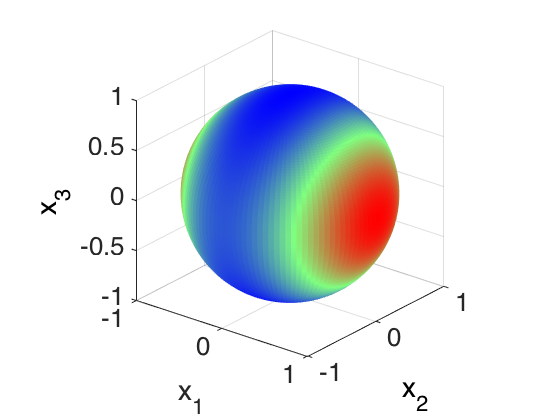
\includegraphics[width=1\textwidth]{Chapter7/images/sphere73.png} 
    \end{center}
    \end{minipage} 
    
    \vspace{12pt} 
    \pause 
    Identify the largest and smallest values of $Q$ on the surface of the sphere, and where they are located. 
    
\end{frame}


\begin{frame}\frametitle{Solution: Largest Value of $Q$ on Sphere}    
    We will identify the largest value of $Q$ on the sphere first. 
    \begin{align*}
        Q =  \vec x\, ^T \spalignmat{9 0 0;0 4 0;0 0 3}\vec x &= 9x_1^2 + 4x_2^2 +3x_3^2 \\
        &\le 9x_1^2 + 9x_2^2 +9x_3^2 \\
        &= \onslide<2->{ 9 (x_1^2 + x_2^2 +x_3^2)} \\
        &= \onslide<3->{9 \lVert \vec x \rVert ^2} \\
        &= \onslide<4->{ 9  }
    \end{align*}
    \onslide<5->{We are only considering points on the surface of the sphere: $\lVert \vec x \rVert ^2 = 1$.  }
\end{frame}


\begin{frame}\frametitle{Solution: Largest and Smallest Values of $Q$ on Sphere}     
    \onslide<2-> {Thus, $$\mathrm{max} \{ Q(\vec x) : ||\vec x|| = 1\} = 9, \ \text{and max occurs at } \vec x = \spalignmat{\pm1;0;0}$$}
    \onslide<3-> {A similar analysis yields 
    $$\mathrm{min} \{ Q(\vec x) : ||\vec x|| = 1\} = 3, \ \text{and min occurs at } \vec x = \spalignmat{0;0;\pm1}$$}
    \onslide<4->{Notice that the minimum and maximum values of $Q$ were the eigenvalues of $A$, and the corresponding eigenvectors gave their locations.}
\end{frame}


\begin{frame}\frametitle{A Constrained Optimization Problem}

    Suppose we wish to find the maximum or minimum values of $$Q(\vec x) = \vec x^{\, T}A \vec x, \quad \vec x \in \mathbb R^n, \quad A \in \mathbb R^{n\times n},$$ subject to $$||\vec x|| = 1$$ \pause That is, we want to find
    \begin{align*}
        m &= \mathrm{min} \{ Q(\vec x) : ||\vec x|| = 1 \} \\
        M &= \mathrm{max} \{ Q(\vec x) : ||\vec x|| = 1 \}
    \end{align*}
    \pause 
    This is an example of a \Emph{constrained optimization} problem. Note that we may also want to know where these extreme values are obtained. 
    
\end{frame}


\begin{frame}\frametitle{Constrained Optimization and Eigenvalues}
    
    \begin{center}\begin{tikzpicture} \node [mybox](box){\begin{minipage}{0.95\textwidth}\vspace{2pt}
    
        If $Q = \vec x^{\, T} A \vec x$, $A$ is a real $n\times n$ symmetric matrix, with eigenvalues 
        $$\lambda_1 \ge \lambda_2 \ldots \ge \lambda_n$$
        and associated normalized eigenvectors 
        $$\vec u_1, \vec u_2, \ldots , \vec u_n$$
        \onslide<2->{Then, subject to the constraint $||\vec x ||=1$, }
        \begin{itemize}
            \item<3-> the \Emph{maximum} value of $Q(\vec x) = \lambda_1$, attained at $\vec x = \pm \, \vec u_1$.
            \item<4-> the \Emph{minimum} value of $Q(\vec x) = \lambda_n$, attained at $\vec x = \pm \, \vec u_n$.
        \end{itemize} 
        
    \end{minipage}};
    \node[fancytitle, right=10pt] at (box.north west) {Theorem};
    \end{tikzpicture}\end{center}
    

\end{frame}


\begin{frame}\frametitle{Proof for Maximum Value of $Q$}
    
    Assume $\lambda_1$ is the largest eigenvalue with corresponding unit eigenvector $\vec u_1$. 
    \begin{align*}
        \onslide<2->{Q = \vec x \,^T A\vec x 
                 &= \vec y\, ^T D\vec y , \quad \text{using } A = PDP^T , \ \vec x = P\vec y\\}
        \onslide<3->{&= \sum \lambda_i y_i^2, \quad \text{because } D \text{ is diagonal} \\}
        \onslide<4->{&\le \sum \lambda_1 y_i^2, \quad \text{because } \lambda_1 \text{ is the largest eigenvalue} \\}
        \onslide<5->{&= \lambda_1 \sum y_i^2 \\}
        \onslide<5->{&= \lambda_1 \, \lVert \vec y \rVert ^2 }
        \onslide<6->{= \lambda_1 , \quad \text{because } \lVert \vec y \rVert ^2 =1 }
    \end{align*}
    \onslide<7->{
    So, the maximum value of $Q$ is at most $\lambda_1$. And $Q = \lambda_1$ at $\pm \vec u_1$ because
    $$Q(\pm \vec u_1) = \vec u_1 \, ^T A \vec u_1 = \vec u_1 \, ^T (\lambda_1 \vec u_1 ) = \lambda_1$$
    }
    
\end{frame}

\frame{\frametitle{Summary}

    \SummaryLine \vspace{4pt}
    \begin{itemize}\setlength{\itemsep}{8pt}

        \item constrained optimization problems of the form: identify the maximum/minimum values (and where they are located) of $$Q(\vec x) = \vec x^{\, T}A \vec x$$ subject to $$||\vec x|| = 1$$
        \item we saw that the maximum/minimum values are given by eigenvalues of $A$
        \item we saw that the locations where these extreme values are given by unit eigenvectors of $A$

    \end{itemize}
    
    \vspace{6pt}
    \pause 
    
}

    % \title{Constrained Optimization with a Repeated Eigenvalue}
\subtitle{\SubTitleName}
\institute[]{\Course}
\author{\Instructor}
\maketitle   
   

\frame{\frametitle{Topics and Objectives}
\Emph{Topics} \\
%\TopicStatement
\begin{itemize}

    \item constrained optimization as an eigenvalue problem
    % \item distance and orthogonality constraints

\end{itemize}

\vspace{0.5cm}

\Emph{Learning Objectives}\\

%\LearningObjectiveStatement

\begin{itemize}

    \item apply eigenvalues and eigenvectors to solve a class of optimization problems that are subject to a distance constraint % and orthogonality constraints.
    
\end{itemize}
} 

\begin{frame}\frametitle{Example}

    Calculate the maximum and minimum values of $Q(\vec x) = \vec x^{\, T}A \vec x$, $\vec x \in \mathbb R^3$, subject to $||\vec x|| = 1$, and identify points where these values are obtained. 
    
    $$Q(\vec x) = x_1^2 + 2x_2x_3$$
\end{frame}
    
\begin{frame}\frametitle{Example Solution}
    
    For $Q(\vec x) = x_1^2 + 2x_2x_3$, we have
    \begin{align*}
        Q &= \vec x \, ^T A\vec x,\quad A = \spalignmat{1 0 0;0 0 1;0 1 0} 
    \end{align*}
    \pause By inspection, $A$ has eigenvalues $\pm 1$ (don't forget that an eigenvalue, $\lambda$, is a number that makes $A - \lambda I$ singular). For $\lambda = 1$, 
    \pause 
    \begin{align*}
        A-I = \spalignmat{0 0 0;0 -1 1;0 1 -1} \Rightarrow \vec v_1 = \spalignmat{1;0;0}, \vec v_2 = \frac{1}{\sqrt2}\spalignmat{0;1;1}
    \end{align*}
\end{frame}
    
\begin{frame}\frametitle{Example Solution}    
    Because $A$ is symmetric, the eigenvector for eigenvalue $\lambda = -1$ must be orthogonal to $\vec v_1$ and $\vec v_2$. \pause So by inspection $$\vec v_3 = \frac{1}{\sqrt{2}}\spalignmat{0;1;-1}$$
    \pause Therefore, the minimum value of $Q$ is $-1$, and is obtained at $\pm \vec v_3$. \pause The maximum value of $Q$ is $+1$, which is obtained at any unit vector in the span of $\vec v_1$ and $\vec v_2$. 
\end{frame}


\begin{frame}\frametitle{Example Solution}    

    The image below is the unit sphere whose surface is colored according to the quadratic from the previous example. Notice the agreement between our solution and the image. 

    \begin{center}
        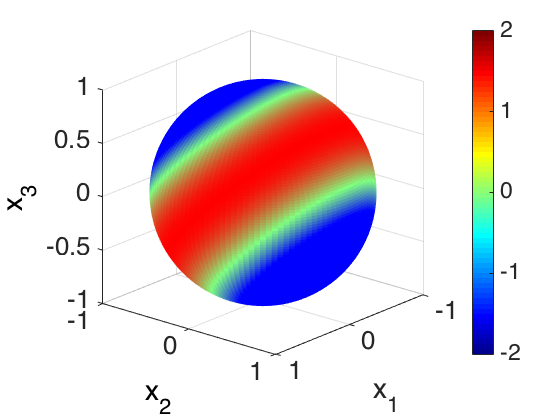
\includegraphics[width=0.5\textwidth]{Chapter7/images/sphere73example2.png} 
    \end{center}

\end{frame}

\frame{\frametitle{Summary}

    \SummaryLine \vspace{4pt}
    \begin{itemize}\setlength{\itemsep}{8pt}

        \item constrained optimization problems of the form: identify the maximum/minimum values (and where they are located) of $$Q(\vec x) = \vec x^{\, T}A \vec x$$ subject to $$||\vec x|| = 1$$
        \item we saw that the maximum/minimum values are given by eigenvalues of $A$
        \item we saw that the locations where these extreme values are given by unit eigenvectors of $A$

    \end{itemize}
    
    \vspace{6pt}

    \pause
}




    % \title{Orthogonality Constraints}
\subtitle{\SubTitleName}
\institute[]{\Course}
\author{\Instructor}
\maketitle   
   

\frame{\frametitle{Topics and Objectives}
\Emph{Topics} \\
%\TopicStatement
\begin{itemize}

    \item constrained optimization as an eigenvalue problem
    \item distance and orthogonality constraints

\end{itemize}

\vspace{0.5cm}

\Emph{Learning Objectives}\\

%\LearningObjectiveStatement

\begin{itemize}

    \item apply eigenvalues and eigenvectors to solve a class of optimization problems that are subject to a distance and orthogonality constraints
    
\end{itemize}
} 




\begin{frame}\frametitle{An Orthogonality Constraint}
    
    \begin{center}\begin{tikzpicture} \node [mybox](box){\begin{minipage}{0.90\textwidth}\vspace{2pt}
    
        Suppose $Q = \vec x^{\, T} A \vec x$, where $A \in \mathbb R^{n\times n}$ is symmetric and has eigenvalues
        $$\lambda_1 \ge \lambda_2 \ldots \ge \lambda_n$$
        and associated eigenvectors
        $$\vec u_1, \vec u_2, \ldots , \vec u_n$$
        \onslide<2->{Subject to the constraints $||\vec x ||=1$ and} \onslide<3->{$\vec x \cdot \vec u_1 = 0$,}
        \begin{itemize}
            \item<4-> the maximum value of $Q(\vec x) = \lambda_{2}$, attained at $\vec x = \vec u_{2}$
            \item<5-> the minimum value of $Q(\vec x) = \lambda_n$, attained at $\vec x = \vec u_n$
        \end{itemize}
        
        % \vspace{6pt} 
        
        % Note that $\lambda_2$ is the second largest eigenvalue of $A$.  
        
    \end{minipage}};
    \node[fancytitle, right=10pt] at (box.north west) {Theorem};
    \end{tikzpicture}\end{center}

\end{frame}

\begin{frame}\frametitle{Outline of the Proof}

    \begin{itemize}
        \item<2-> The proof of this theorem uses a similar approach to the theorem that gives the maximum of $Q$ subject to $\lVert \vec x \rVert = 1$. 
        \item<3-> We would use a change of variable, and express $Q$ using a diagonal matrix and an orthonormal basis for $\mathbb R^n$. 
        \item<4-> In fact, we could use this approach to identify maximum values with additional orthogonality constraints. This would go beyond the scope of what we need. 
    \end{itemize}
    
\end{frame}

\begin{frame}\frametitle{Example}

    Calculate the maximum value of $Q(\vec x) = \vec x^{\, T}A \vec x$, $\vec x \in \mathbb R^3$, subject to $||\vec x|| = 1$ and to $\vec x \cdot \vec u_1 = 0$, and identify a point where this maximum is obtained. 
    
    $$Q(\vec x) = x_1^2 + 2x_2x_3, \qquad \vec u_1 = \spalignmat{1;0;0}$$

\end{frame}

\frame{\frametitle{Summary}

    \SummaryLine \vspace{4pt}
    \begin{itemize}\setlength{\itemsep}{8pt}

        \item constrained optimization problems of the form: identify the maximum/minimum values (and where they are located) of $$Q(\vec x) = \vec x^{\, T}A \vec x$$ subject to $$||\vec x|| = 1, \ \text{and} \ \vec x \cdot u_1 = 0$$
        \item we saw that the maximum/minimum values are given by eigenvalues of $A$
        \item we saw that the locations where these extreme values are given by unit eigenvectors of $A$

    \end{itemize}
    
    \vspace{6pt}
}

    % \title{Singular Values}
\subtitle{\SubTitleName}
\institute[]{\Course}
\author{\Instructor}
\maketitle   


\frame{\frametitle{Topics and Objectives}
\Emph{Topics} \\
%\TopicStatement
\begin{itemize}

    \item singular values of a matrix
    \item the connection between linear transforms, constrained optimization, and singular values 
    % \item the Singular Value Decomposition (SVD) and some of its applications

\end{itemize}

\vspace{0.5cm}

\Emph{Learning Objectives}\\

%\LearningObjectiveStatement

\begin{itemize}

    \item compute the singular values of a matrix
    \item interpret the singular values of a matrix in terms of a constrained optimization problem related to linear transforms
    % \item Compute the SVD for a rectangular matrix
    % \item Apply the SVD to 
    % \begin{itemize} 
    %     \item estimate the rank and condition number of a matrix, 
    %     \item construct a basis for the four fundamental spaces of a matrix, and
    %     \item construct a spectral decomposition of a matrix.
    % \end{itemize}
\end{itemize}

} 






\begin{frame}\frametitle{Singular Values}


    \begin{center}\begin{tikzpicture} \node [mybox](box){\begin{minipage}{0.62\textwidth}\vspace{4pt}
    
        The singular values of any $m\times n$ real matrix $A$ are the square roots of the eigenvalues of $A^TA$. 
        
    \end{minipage}};\node[fancytitle, right=10pt] at (box.north west) {\textbf{Definition}};\end{tikzpicture}\end{center}
    
    \vspace{6pt}
    
    \pause
    
    \onslide<2->{\Emph{Questions}}
    \begin{itemize}
        \item<2-> How might this definition connect to some of the other topics we covered? 
        \item<3-> How might singular values be viewed from a more geometric perspective? 
        \item<4-> Can the eigenvalues of $A^TA$ be negative? 
        \item<5-> What problems can singular values be used to solve? 
    \end{itemize}
    
    \vspace{12pt}
    \onslide<6->{These questions are explored throughout this presentation. }
    
\end{frame}



\begin{frame} \frametitle{Linear Transforms on the Unit Circle}

    \pause 
    The linear transform whose standard matrix is $$A = \frac{1}{\sqrt{2}}\spalignmat{1 -1;1 1}\spalignmat{2\sqrt{2} 0;0 \sqrt{2}} = \spalignmat{2 -1;2 1}$$ \pause transforms unit vectors in $\mathbb R^2$ to an ellipse, as shown below. 
    \pause 
    \vspace{-12pt}
    
    \begin{columns}
        \begin{column}{.1\textwidth}
        \end{column}
        \begin{column}{.3\textwidth}
        \begin{center}
            \begin{tikzpicture}[scale=0.6]
                \draw[->,gray] (-2,0) -- (2,0) node[right,black] {$x_1$};
                \draw[->,gray] (0,-2) -- (0,2) node[left,black] {$x_2$};
                \draw [rotate=0,black,very thick] (0,0) ellipse (30pt and 30pt);  
            \end{tikzpicture}
        \end{center}
        \end{column}        
        \begin{column}{.2\textwidth}
        \vspace{1cm}
        \begin{center}
            \begin{tikzpicture}[scale=0.95]
                \draw[->,thick,>=stealth,line width=0.75mm] (-3,0) -- node[above] {multiply by $A$} ++ (2,0);
            \end{tikzpicture}
        \end{center}
        \end{column}     
        \begin{column}{.3\textwidth}
        \begin{center}
            \begin{tikzpicture}[scale=0.6]
                \draw[->,gray] (-2,0) -- (2,0) node[right,black] {$x_1$};
                \draw[->,gray] (0,-2) -- (0,2) node[left,black] {$x_2$};
                \draw [rotate=45,black,very thick] (0,0) ellipse (60pt and 40pt);  
            \end{tikzpicture}
        \end{center}
        \end{column}       
        \begin{column}{.1\textwidth}
        \end{column}        
    \end{columns}
    
    \vspace{6pt}
    \pause \begin{center}
        What unit vector, $\vec v$, maximizes $||A \vec v||$? What is $||A \vec v||$ equal to? 
    \end{center}
\end{frame}



\begin{frame} \frametitle{Solution}

    Our goal is to maximize $\lVert A\vec v \rVert$ subject to $\lVert \vec v \rVert = 1$, in other words, 
    $$\max_{\lVert \vec v \rVert = 1}\lVert A\vec v \rVert$$
    \pause But the maximum occurs at the same location as $\lVert A\vec v \rVert^2$. 
    \begin{align*}
        \lVert A\vec v \rVert^2 = \vec v\,^T A^TA \vec v
    \end{align*}
    \pause
    $A^TA$ is symmetric.
    
    \pause 
    \vspace{12pt}
    \textit{We can answer some our questions with the eigenvalues of $A^TA$. }
\end{frame}



\begin{frame} \frametitle{Solution}
    We need the eigenvalues of $A^TA$. 
    \begin{align*}
        A^TA  = \spalignmat{2 2;-1 1}\spalignmat{2 -1;2 1} = \spalignmat{8 0;0 2} \quad \Rightarrow \quad \lambda = 8, 2
    \end{align*}
    Thus, 
    $$\max_{\lVert \vec v \rVert = 1}\lVert A\vec v \rVert^2 = 8$$
    So
    $$\max_{\lVert \vec v \rVert = 1}\lVert A\vec v \rVert = \sqrt8$$
    Thus, $\sqrt8$ is the maximum value that we were seeking. 
    
    \vspace{12pt}
    
    Next: what is the $\vec v$ that corresponds to this maximum? 

\end{frame}



\begin{frame} \frametitle{Solution}
    The unit eigenvector corresponding to the largest eigenvalue is the vector, $\vec v_1$, that maximizes $\lVert A\vec v \rVert$. 
    
    $$A^TA - \lambda I = \spalignmat{0 0;0 -6} \quad \Rightarrow \quad \vec v_1 = \spalignmat{1;0}$$
    
    The unit vector that maximizes $\lVert A\vec v \rVert$ is $\vec v_1 = \spalignmat{1;0}$.
\end{frame}



\begin{frame} \frametitle{Solution}    
    Recall that $A$ is the standard matrix for a transform that rotates and scales.
    
    $$A = \frac{1}{\sqrt{2}}\spalignmat{1 -1;1 1}\spalignmat{2\sqrt{2} 0;0 \sqrt{2}} = \spalignmat{2 -1;2 1}$$
    \vspace{-18pt}
        \begin{columns}
        \begin{column}{.1\textwidth}
        \end{column}
        \begin{column}{.3\textwidth}
        \begin{center}
            \begin{tikzpicture}[scale=0.8]
                \draw[->,gray] (-2,0) -- (2,0) node[right,black] {$x_1$};
                \draw[->,gray] (0,-2) -- (0,2) node[left,black] {$x_2$};
                \draw [rotate=0,black,very thick] (0,0) ellipse (30pt and 30pt);  
                \draw[->,thick,>=stealth,DarkRed,line width=0.75mm] (0,0) -- node[above] {$\vec v_1$} ++ (1,0);
            \end{tikzpicture}
        \end{center}
        \end{column}        
        \begin{column}{.2\textwidth}
        \vspace{1cm}
        \begin{center}
            \begin{tikzpicture}[scale=0.95]
                \draw[->,thick,>=stealth,line width=0.75mm] (-3,0) -- node[above] {multiply by $A$} ++ (2,0);
            \end{tikzpicture}
        \end{center}
        \end{column}     
        \begin{column}{.3\textwidth}
        \begin{center}
            \begin{tikzpicture}[scale=0.8]
                \draw[->,gray] (-2,0) -- (2,0) node[right,black] {$x_1$};
                \draw[->,gray] (0,-2) -- (0,2) node[left,black] {$x_2$};
                \draw [rotate=45,black,very thick] (0,0) ellipse (60pt and 40pt);  
                \draw[->,thick,>=stealth,DarkRed,line width=0.75mm] (0,0) -- (1.52,1.52);
                \draw[DarkRed] (1.6,1.6) node[right] {$A\vec v_1$} ;
            \end{tikzpicture}
        \end{center}
        \end{column}       
        \begin{column}{.1\textwidth}
        \end{column}        
    \end{columns}
    \begin{center}
            The length of $A\vec v_1$ is the square root of the largest eigenvalue of $A^TA$, or $\sqrt 8$.
    \end{center}    
\end{frame}


\begin{frame} \frametitle{The Smallest Eigenvalue}    
    A similar process yields that the smallest eigenvalue of $A^TA$ is
    
    $$ \min_{\lVert \vec v \rVert = 1}\lVert A\vec v \rVert = \sqrt{2}, \quad \vec v_2 = \spalignmat{0;1}$$
    
    \pause
    

    \vspace{-6pt}
        \begin{columns}
        \begin{column}{.1\textwidth}
        \end{column}
        \begin{column}{.3\textwidth}
        \begin{center}
            \begin{tikzpicture}[scale=0.8]
                \draw[->,gray] (-2,0) -- (2,0) node[right,black] {$x_1$};
                \draw[->,gray] (0,-2) -- (0,2) node[left,black] {$x_2$};
                \draw [rotate=0,black,very thick] (0,0) ellipse (30pt and 30pt);  
                \draw[->,thick,>=stealth,DarkRed,line width=0.75mm] (0,0) -- node[above] {$\vec v_1$} ++ (1,0);
                \draw[->,thick,>=stealth,DarkBlue,line width=0.75mm] (0,0) -- ++ (0,1);
                \draw[DarkBlue] (-.5,0.9) node[above] {$\vec v_2$} ;
            \end{tikzpicture}
        \end{center}
        \end{column}        
        \begin{column}{.2\textwidth}
        \vspace{1cm}
        \begin{center}
            \begin{tikzpicture}[scale=0.95]
                \draw[->,thick,>=stealth,line width=0.75mm] (-3,0) -- node[above] {multiply by $A$} ++ (2,0);
            \end{tikzpicture}
        \end{center}
        \end{column}     
        \begin{column}{.3\textwidth}
        \begin{center}
            \begin{tikzpicture}[scale=0.8]
                \draw[->,gray] (-2,0) -- (2,0) node[right,black] {$x_1$};
                \draw[->,gray] (0,-2) -- (0,2) node[left,black] {$x_2$};
                \draw [rotate=45,black,very thick] (0,0) ellipse (60pt and 40pt);  
                \draw[->,thick,>=stealth,DarkRed,line width=0.75mm] (0,0) -- (1.52,1.52);
                \draw[->,thick,>=stealth,DarkBlue,line width=0.75mm] (0,0) -- (-1.,1.);                
                \draw[DarkRed] (1.6,1.6) node[right] {$A\vec v_1$} ;
                \draw[DarkBlue] (-1.3,1.1) node[above] {$A\vec v_2$} ;
            \end{tikzpicture}
        \end{center}
        \end{column}       
        \begin{column}{.1\textwidth}
        \end{column}        
    \end{columns}
    \begin{center}
    \pause 
            $\lVert A\vec v_2 \rVert$ is the square root of the smallest eigenvalue of $A^TA$, which is $\sqrt 2$.
            
         
    \end{center}    
\end{frame}


\begin{frame} \frametitle{Singular Values are the Eigenvalues of $A^TA$}    

    Let $\sigma_1 = \sqrt{\lambda_1} = \sqrt{8}$, and $\sigma_2 = \sqrt{\lambda_2}= \sqrt{2}$. 
    
    \vspace{-6pt}
        \begin{columns}
        \begin{column}{.1\textwidth}
        \end{column}
        \begin{column}{.3\textwidth}
        \begin{center}
            \begin{tikzpicture}[scale=0.8]
                \draw[->,gray] (-2,0) -- (2,0) node[right,black] {$x_1$};
                \draw[->,gray] (0,-2) -- (0,2) node[left,black] {$x_2$};
                \draw [rotate=0,black,very thick] (0,0) ellipse (30pt and 30pt);  
                \draw[->,thick,>=stealth,DarkRed,line width=0.75mm] (0,0) -- node[above] {$\vec v_1$} ++ (1,0);
                \draw[->,thick,>=stealth,DarkBlue,line width=0.75mm] (0,0) -- ++ (0,1);
                \draw[DarkBlue] (-0.5,0.9) node[above] {$\vec v_2$} ;
            \end{tikzpicture}
        \end{center}
        \end{column}        
        \begin{column}{.2\textwidth}
        \vspace{1cm}
        \begin{center}
            \begin{tikzpicture}[scale=0.95]
                \draw[->,thick,>=stealth,line width=0.75mm] (-3,0) -- node[above] {multiply by $A$} ++ (2,0);
            \end{tikzpicture}
        \end{center}
        \end{column}     
        \begin{column}{.3\textwidth}
        \begin{center}
            \begin{tikzpicture}[scale=0.8]
                \draw[->,gray] (-2,0) -- (2,0) node[right,black] {$x_1$};
                \draw[->,gray] (0,-2) -- (0,2) node[left,black] {$x_2$};
                \draw [rotate=45,black,very thick] (0,0) ellipse (60pt and 40pt);  
                \draw[->,thick,>=stealth,DarkRed,line width=0.75mm] (0,0) -- (1.52,1.52);
                \draw[->,thick,>=stealth,DarkBlue,line width=0.75mm] (0,0) -- (-1.,1.);                
                \draw[DarkRed] (1.6,1.6) node[right] {$A\vec v_1$} ;
                \draw[DarkBlue] (-1.3,1.1) node[above] {$A\vec v_2$} ;
                
                \onslide<2->{\draw[DarkRed] (0.7,0.6) node[right] {$\sigma_1$} ;}
                \onslide<3->{\draw[DarkBlue] (-0.7,-0.16) node[above] {$\sigma_2$} ; }              
            \end{tikzpicture}
        \end{center}
        \end{column}       
        \begin{column}{.1\textwidth}
        \end{column}        
    \end{columns}
    \begin{center}
    \onslide<4->{In other words: the length of $A\vec v_i$ is the square root of the eigenvalues of $A^TA$, or $\sqrt{\lambda_i}$.}
    \end{center}    
\end{frame}








\begin{frame}\frametitle{Eigenvalues of $A^TA$ Are Non-Negative}

    \vspace{-12pt}

    \begin{center}\begin{tikzpicture} \node [mybox](box){\begin{minipage}{0.55\textwidth}\vspace{4pt}
    
        The eigenvalues of $ A ^{T} A $ are non-negative. 
        
    \end{minipage}};\node[fancytitle, right=10pt] at (box.north west) {\textbf{Theorem}};\end{tikzpicture}\end{center}
    
    \vspace{6pt}
    
    \pause
    
    \Emph{Proof}: recall that $\vec v_j^T\vec v_j = \vec v_j\cdot\vec v_j = \lVert \vec v_j \rVert ^2 =1$ because $\vec v_j$ are \Emph{unit} eigenvectors of $A^TA$.  
    \pause 
    \begin{align*}
        \lVert A \vec v_j\rVert ^2 =
        (A \vec v_j) ^{T} A \vec v_j= \vec v_j A^T A \vec v_j = \lambda _j \vec v_j ^T \vec v_j = \lambda _j \geq 0. 
    \end{align*}
    \pause 
    Therefore: \pause
    \begin{itemize}
        \item the eigenvalues of $A^TA$ must be real and non-negative
        \item the singular values of $A$, which are the square roots of the eigenvalues, must also be real and non-negative
    \end{itemize} 
    


\end{frame}









% \begin{frame}\frametitle{Singular Values}
    
%     % The matrix $ A ^{T} A $ is always symmetric, with non-negative eigenvalues $ \lambda _1 \geq \lambda _2 \geq \cdots \geq \lambda _n \geq 0$.  Let $ \{\vec v_1 ,\dotsc, \vec v_n\}$ be the associated orthonormal eigenvectors.  

%     % \vspace{12pt} 
    
%     Earlier in this presentation we saw that the largest singular value of $A$ is:\pause the maximum length of $A\vec v$ subject to $\lVert \vec v \rVert =1$. \pause
    
%     $$\sigma_1 = \max_{\lVert \vec v \rVert = 1}\lVert A\vec v \rVert$$
    
%     \vspace{12pt}
%     \pause 
%     What about the other singular values? 
% \end{frame}


% \begin{frame}\frametitle{Singular Values}    
%     \begin{itemize}
%         \item Recall that the second largest eigenvalue of a symmetric matrix gives the maximum of $\lVert A\vec v \rVert$ subject to $$ \lVert \vec v \rVert =1 , \quad \vec v \cdot \vec u_1 = 0$$
%         \item The second largest eigenvalue is $\sigma_2$
%         \item Thus, $\sigma_2$ 
%     \end{itemize}
%     Likewise with the remaining eigenvalues. 
% \end{frame}






\begin{frame}\frametitle{Note: Singular Values are Ordered}

    %  The matrix $ A ^{T} A $ is always symmetric, with non-negative eigenvalues $ \lambda _1 \geq \lambda _2 \geq \cdots \geq \lambda _n \geq 0$. 
    Because the eigenvalues of $A^TA$ are non-negative, the singular values of $A$ must also be real and non-negative. \pause They can be ordered from largest to smallest. 
    
    \pause 

    \begin{center}\begin{tikzpicture} \node [mybox](box){\begin{minipage}{0.95\textwidth}\vspace{4pt}
    
        The singular values, $\sigma_j$, of any $m\times n$ real matrix $A$ are the square roots of the eigenvalues of $A^TA$. Singular values are arranged in decreasing order.
        
        $$\sigma _1 = \sqrt {\lambda _1 } \geq \sigma _2 = \sqrt {\lambda _2}  \geq \ \cdots \ \geq \sigma _n=\sqrt {\lambda _n} $$ 
        
    \end{minipage}};\node[fancytitle, right=10pt] at (box.north west) {\textbf{Definition}};\end{tikzpicture}\end{center}
    
    \vspace{6pt}
    This is a standard convention for singular values. 
    
    
    
    
\end{frame}


\begin{frame}\frametitle{Singular Values are Lengths}

    It also follows from the previous slide that the singular values of $A$ represent lengths of vectors in $\mathbb R^n$. That is, when showing that the eigenvalues of $A^TA$ are non-negative, we saw that
    \onslide<2->{ $$|| A\vec v_i||^2 = \lambda_i $$}
    \onslide<3->{ Therefore, $$|| A\vec v_i||= \sigma_i $$}
    \onslide<4->{We make use of this relationship when constructing the SVD of a matrix. }
\end{frame}







\frame{\frametitle{Summary}

    \SummaryLine \vspace{4pt}
    \begin{itemize}\setlength{\itemsep}{8pt}

        \item the singular values of any $m\times n$ real matrix $A$ are the square roots of the eigenvalues of $A^TA$
        \item singular values are related to the lengths of $\lVert A \vec x \rVert$ for $\lVert \vec x \rVert = 1$
        \item singular values are real and non-negative
        \item singular values are arranged in decreasing order

    \end{itemize}
    
    \vspace{6pt}
}
 % done! 
    % \title{Singular Vectors}
\subtitle{\SubTitleName}
\institute[]{\Course}
\author{\Instructor}
\maketitle   


\frame{\frametitle{Topics and Objectives}
\Emph{Topics} \\
%\TopicStatement
\begin{itemize}

    \item singular vectors (the eigenvectors of $A^TA$)

\end{itemize}

\vspace{0.5cm}

\Emph{Learning Objectives}\\

%\LearningObjectiveStatement

\begin{itemize}
    \item apply the eigenvectors of $A^TA$ to construct a basis for $\Col A$, $\Row A$, and $\Nul A$
    \item determine the rank of a matrix using the singular values of that matrix
\end{itemize}

} 

\begin{frame}{Motivation: The Four Fundamental Subspaces}

    \begin{center}\begin{tikzpicture} \node [mybox](box){\begin{minipage}{0.85\textwidth}\vspace{2pt}
    For any $ A \in \mathbb R^{m\times n}$,  the orthogonal complement of $\Row A$ is $ \Null A$, and the orthogonal complement of $ \Col A$ is  $ \Null A ^{T}$.  

    \end{minipage}};
    \node[fancytitle, right=10pt] at (box.north west) {Theorem (The Four Subspaces)};
    \end{tikzpicture}\end{center}

    % The idea behind this theorem is described in the diagram below. 
    \pause 
    
    \begin{center}
    \begin{tikzpicture}[scale=.65]
        
        \onslide<2->{
        % boxes
        \filldraw[draw=DarkBlue!50,fill=DarkBlue!15] (0,0) -- (-1,1) -- (1,3) -- (2,2) -- cycle;
        \filldraw[draw=DarkBlue!50,fill=DarkBlue!15] (0,0) -- (1,-1) -- (0,-2) -- (-1,-1) -- cycle;      
        \draw (0.4, 1.7) node[below]{\small $\Row A$};
        \draw (0.0,-0.7) node[below]{\small $\Nul A$};        
        }
        
        \onslide<3->
        {
        \filldraw[draw=DarkGreen!50,fill=DarkGreen!15] (4,0) -- (2.5, 1.5) -- (3.5, 2.5) -- (5,1) -- cycle;
        \filldraw[draw=DarkGreen!50,fill=DarkGreen!15] (4,0) -- (5.5,-1.5) -- (4.5,-2.5) -- (3,-1) -- cycle;        
        \draw (3.9, 1.5) node[below]{\small $\Col A$};
        \draw (4.2, -0.8) node[below]{\small $\Nul A^T$};        
        }

        \onslide<4->{
        \draw (-1.0,0.5) node[below]{\Large $\color{DarkBlue} \mathbb R^n$};
        }

        \onslide<5->{
        \draw ( 5.2,0.5) node[below]{\Large $\color{DarkGreen} \mathbb R^m$};
        }
        
    \end{tikzpicture}
    \end{center}
    \pause 
    The eigenvectors of $A^TA$ can be used construct bases for these subspaces. 
\end{frame}

\begin{frame}\frametitle{Orthogonal Bases for $\Nul A$ and $\Row A$}

    \begin{center}\begin{tikzpicture} \node [mybox](box){\begin{minipage}{0.94\textwidth}\vspace{2pt}
        
        Suppose $\vec v_i$ are the $n$ orthogonal eigenvectors of $A^TA$, ordered so that their corresponding eigenvalues satisfy $\lambda_1 \ge \lambda_2 \ge \ldots \ \ge \lambda_n$. \onslide<2->{Suppose also that $A$ has $r$ non-zero singular values, $r \le n$. }\onslide<3->{Then the set of vectors $$\{\vec v_{r+1},  \vec v_{r+2}, \ \ldots \ , \vec v_n\}$$ is an orthogonal basis for $\Nul A$, and the set $$\{\vec v_{1},  \vec v_{2}, \ \ldots \ , \vec v_r\}$$ is an orthogonal basis for $\Row A$, and $\text{rank} A = r$. }
    \end{minipage}};
    \node[fancytitle, right=10pt] at (box.north west) {Theorem};
    \end{tikzpicture}\end{center}

\end{frame}

\begin{frame}\frametitle{Proof For Orthogonal Basis for $\Nul A$}

    \Emph{Outline of the Proof}\\ 
    For a set of vectors to form an orthogonal basis for a subspace they must be in that space, span the space, be independent, and mutually orthogonal.
    \begin{itemize}
        \item<2-> Each $\vec v_i$ is an eigenvector, so none of them are the zero vector. 
        \item<3-> $\vec v_i$ are orthogonal and span $\mathbb R^n$ (they are eigenvectors of a symmetric matrix, $A^TA$).
        \item<4-> Recall that the lengths of $A\vec v_i$ are the singular values of $A$:
        $$\lVert A\vec v_i \rVert = \sigma _i.$$ 
        \item<5-> Then if $\lVert A\vec v_i \rVert =  0$ for $i > r$, then $\vec v_i \in \Nul A$ for $i > r$.
        \item<6-> Then if $\lVert A\vec v_i \rVert \ne  0$ for $i \le r$, then $\vec v_i $ cannot be in $\Nul A$ for $i \le r$, they must be in $(\Nul A)\Perp = \Row A$, because $\{\vec v_i\}$ is an orthonormal set. 
    \end{itemize}

\end{frame}

\begin{frame}\frametitle{Proof For Orthogonal Basis for $\Nul A$}

    Thus, our basis for $\Nul A$ is the set  $$\{\vec v_{r+1},  \vec v_{r+2}, \ \ldots \ , \vec v_n\}$$ and our basis for $\Row A$ is the set $$\{\vec v_{1},  \vec v_{2}, \ \ldots \ , \vec v_r\}$$
    We must also describe why $\Rank A = r$. 
    \begin{itemize}
        \item<2-> There are $r$ vectors in our basis for $\Row A$.
        \item<3-> Recall that $\dim(\Row A) = \dim(\Col A) = \Rank A$.
    \end{itemize}
    \onslide<5->{Thus, $\Rank A$ is the number of non-zero singular values, $r$. }
\end{frame}



\begin{frame}\frametitle{Orthogonal Bases for $\Col A$ and $\Nul A^T$}

    \begin{center}\begin{tikzpicture} \node [mybox](box){\begin{minipage}{0.90\textwidth}\vspace{2pt}
        
        Suppose $\vec v_i$ are the $n$ orthonormal eigenvectors of $A^TA$, ordered so that their corresponding eigenvalues satisfy $\lambda_1 \ge \lambda_2 \ge \ldots \ \ge \lambda_n$. \onslide<2->{Suppose also that $A$ has $r$ non-zero singular values. }\onslide<3->{Then $$\{A\vec v_1, A\vec v_2, \ \ldots \ , A\vec v_r\}$$ are an orthogonal basis for $\Col A$.}
    \end{minipage}};
    \node[fancytitle, right=10pt] at (box.north west) {Theorem};
    \end{tikzpicture}\end{center}


\end{frame}

\begin{frame}\frametitle{Orthogonal Bases for $\Col A$ and $\Nul A^T$}

    \Emph{Outline of the Proof}\\ 

    \begin{itemize}
        \item<2-> Each $A\vec v_i$ is a vector in $\Col A$.
        \item<3-> $A\vec v_i$ and $A\vec v_j$ are orthogonal: 
        $$(A\vec v_i) \cdot (A\vec v_j) = \vec v_i^T A^T A \vec v_j = \lambda_j \vec v_i \cdot \vec v_j = 0 $$
        \item<4-> For $i \le r = \Rank A$, $A\vec v_i$ are orthogonal and non-zero. So they must also independent and form an orthogonal basis for $\Col A$.
    \end{itemize}
    \onslide<5->{Note that for $i > r$, $A\vec v_i = \vec 0$ because $\vec v_i \in \Nul A$ for $i > r$. }

\end{frame}


\begin{frame}{Summary: The Four Fundamental Spaces}

    Suppose $\vec i$ are orthonormal eigenvectors for $A^TA$, and $$\vec u _i = \frac{1}{\sigma_i}A\vec v_ i \ \text{ for } i \le r = \Rank A, \ \sigma_i = \lVert A \vec v_i \rVert.$$ \onslide<2->{Then we have the following orthogonal bases for any $m\times n$ real matrix $A$. }
    \begin{itemize}
    
        \item<3->  $ \vec v_1 ,\dotsc, \vec v_r$ is an orthonormal basis for $ \Row A$. 
        
        \item<4->  $ \vec v_{r+1} ,\dotsc, \vec v_n$ is an orthonormal basis for $ \Nul  A $. 
        
        \item<5->  $ \vec u_1 ,\dotsc, \vec u_r$ is an orthonormal basis for $ \Col A$.  
        
        % \item  $ \vec u_{r+1} ,\dotsc, \vec u_n$ is an orthonormal basis for $ \Nul  A ^{T}$. 
        
    \end{itemize}

    \vspace{12pt} 
    
    \onslide<6->{If we need a basis for $(\Col A)\Perp$, what might we do?} \onslide<7->{One approach: identify any $m-r$ independent non-zero vectors in $(\Col A)\Perp$ and then use Gram-Schmidt to orthogonalize them (more on this later).}
    
\end{frame}


\begin{frame}{Summary: The Four Fundamental Spaces}
%\begin{gather*}\textup{dim} (\textup{Col} A) = \textup{dim} (\textup{Row} A) = r 
%\\
%\Nul  A = (\textup{Row} A), \qquad \Nul  A ^{T} = (\textup{Col} A).\end{gather*}

\begin{center}
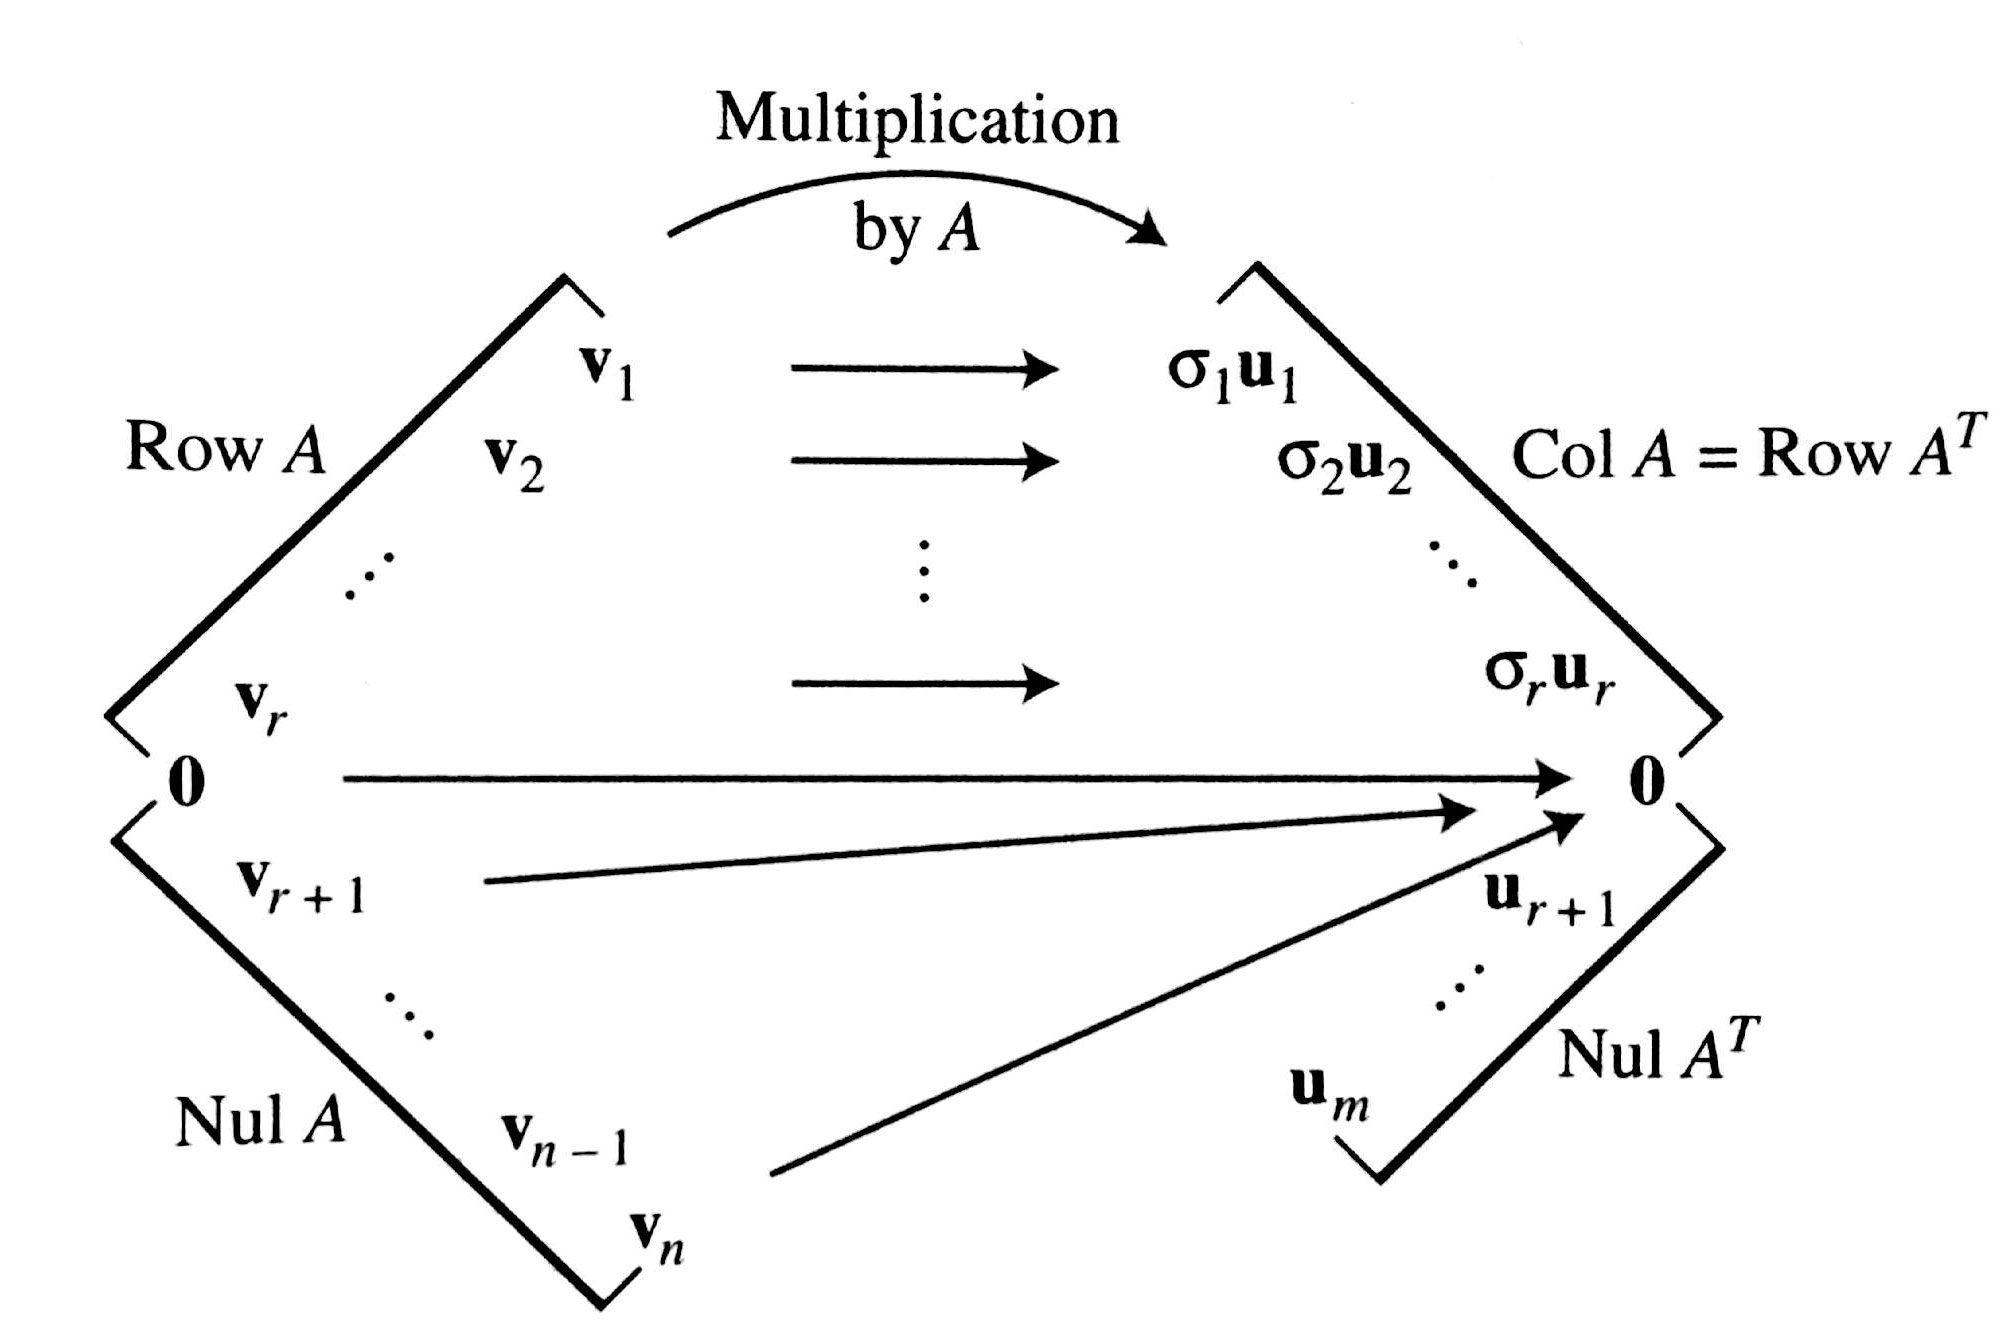
\includegraphics[width=0.6\textwidth]{Chapter7/images/image005.jpg} 
\end{center}


\end{frame}



\begin{frame}\frametitle{The Left and Right Singular Vectors}

    \begin{center}\begin{tikzpicture} \node [mybox](box){\begin{minipage}{0.840\textwidth}\vspace{2pt}
        
        The vectors $\{\vec u_i\}$ for $i \le m$ are the \Emph{left singular vectors} of $A$. 
        The vectors $\{\vec v_i\}$ for $i \le n$ are the \Emph{right singular vectors} of $A$. 
    \end{minipage}};
    \node[fancytitle, right=10pt] at (box.north west) {Definition};
    \end{tikzpicture}\end{center}
    
    \vspace{6pt}

    \onslide<2->{\textit{The reason we refer to these vectors as left and right singular vectors is connected to the singular value decomposition (more on this later).} }
    
\end{frame}



\begin{frame}\frametitle{Examples}

    Suppose $A$ is a $12\times4$ real matrix and has 3 non-zero singular values. Indicate whether the following statements are true or false. 
    \begin{enumerate}
        \item<2-> A basis for $\Col A$ is given by the vectors $A\vec v_1$, $A\vec v_2$, and $A\vec v_3$. 
        \item<2-> A basis for $\Nul A$ is given by $\vec v_1$, $\vec v_2$, and $\vec v_3$. 
    \end{enumerate}
    \vspace{12pt}
    \Emph{Solutions}
    \begin{enumerate}
        \item<3-> True: $A$ has rank 3, the three left singular vectors $A\vec v_1$, $A\vec v_2$, and $A\vec v_3$ are independent and are in $\Col A$, so they form a basis for $\Col A$. 
        \item<4-> False: $A$ has rank 3, so the three right singular vectors $\vec v_1$, $\vec v_2$, and $\vec v_3$ form a basis for $\Row A$. The vector $\vec v_4$ forms a basis for $\Nul A$. 
    \end{enumerate}

\end{frame}



\frame{\frametitle{Summary}

    \SummaryLine \vspace{4pt}
    \begin{itemize}\setlength{\itemsep}{8pt}
        \item the eigenvectors of $A^TA$
        \item constructing a basis for $\Col A$, $\Row A$, and $\Nul A$
        \item determine the rank of a matrix using the singular values of that matrix
    \end{itemize}
    
    \vspace{6pt}
}




    % \title{The SVD}
\subtitle{\SubTitleName}
\institute[]{\Course}
\author{\Instructor}
\maketitle   


\frame{\frametitle{Topics and Objectives}
\Emph{Topics} \\
%\TopicStatement
\begin{itemize}

    \item the Singular Value Decomposition (SVD) of a matrix and how to compute the SVD for a given matrix % and some of its applications

\end{itemize}

\vspace{0.5cm}

\Emph{Learning Objectives}\\

%\LearningObjectiveStatement

\begin{itemize}

    \item compute the SVD for a rectangular matrix
    % \item Apply the SVD to 
    % \begin{itemize} 
    %     \item estimate the rank and condition number of a matrix, 
    %     \item construct a basis for the four fundamental spaces of a matrix, and
    %     \item construct a spectral decomposition of a matrix.
    % \end{itemize}
\end{itemize}

} 



\begin{frame}\frametitle{The SVD}

    \begin{center}\begin{tikzpicture} \node [mybox](box){\begin{minipage}{0.90\textwidth}\vspace{2pt}
        Suppose $A$ is an $ m \times n$ matrix with singular values $ \sigma_1 \geq \sigma _2 \geq \cdots \geq \sigma _n  $ and $m \ge n$. \onslide<2->{Then $A$ has the decomposition $A = U \Sigma V ^{T}$ where }\onslide<3->{
        \begin{equation*}
            \Sigma = \spalignmat{D;\mathbf{0}_{m-n,n}}, \
            D = 
            \begin{pmatrix}
                \sigma _1 & 0 & \ldots & 0   
                \\
                0 & \sigma _2 & \ldots   &  \vdots 
                \\
                \vdots & \vdots & \ddots & \vdots
                \\
                0 & 0& \ldots & \sigma _n  
            \end{pmatrix}
        \end{equation*} }
        \onslide<4->{$U$ is a $ m \times m $ orthogonal matrix, and $ V $ is a $ n \times n$ orthogonal matrix. }\onslide<5->{If $m < n$, then $\Sigma = \spalignmat{D \mathbf0_{m,n-m}}$ with everything else the same. }
    \end{minipage}};
    \node[fancytitle, right=10pt] at (box.north west) {Theorem: Singular Value Decomposition};
    \end{tikzpicture}\end{center}


\end{frame}







\begin{frame}\frametitle{Proof That $A = U\Sigma V^T$}

    Our proof is similar to the proof for diagonalization. We construct $V = (\vec v_1 \ \vec v_2 \ \ldots  \vec v_n)$ and set $$\sigma_i \vec u_i = A \vec v_i, \quad \sigma_i = \lVert A \vec v_i \rVert $$
    \begin{align*}
        \text{Thus: } \onslide<2->{AV = A(\vec v_1 \ \vec v_2 \ \ldots \ \vec v_n) &= (A\vec v_1 \ A\vec v_2 \ \ldots  A\vec v_n) \\}
        \onslide<4->{&= (\sigma_1\vec u_1 \ \sigma_2\vec u_2 \ \ldots \  \sigma_n\vec u_n) \\}
        \onslide<5->{&= (\vec u_1 \ \vec u_2 \ \ldots \ \vec u_n)\spalignmat{\sigma_1,,;,\ddots,;,,\sigma_n} = U\Sigma}
    \end{align*}
    \onslide<6->{Thus, $AV = U \Sigma$, or $A=U\Sigma V^T$. }
    
\end{frame}




\begin{frame}{The SVD and Linear Transforms}
    \begin{center}
    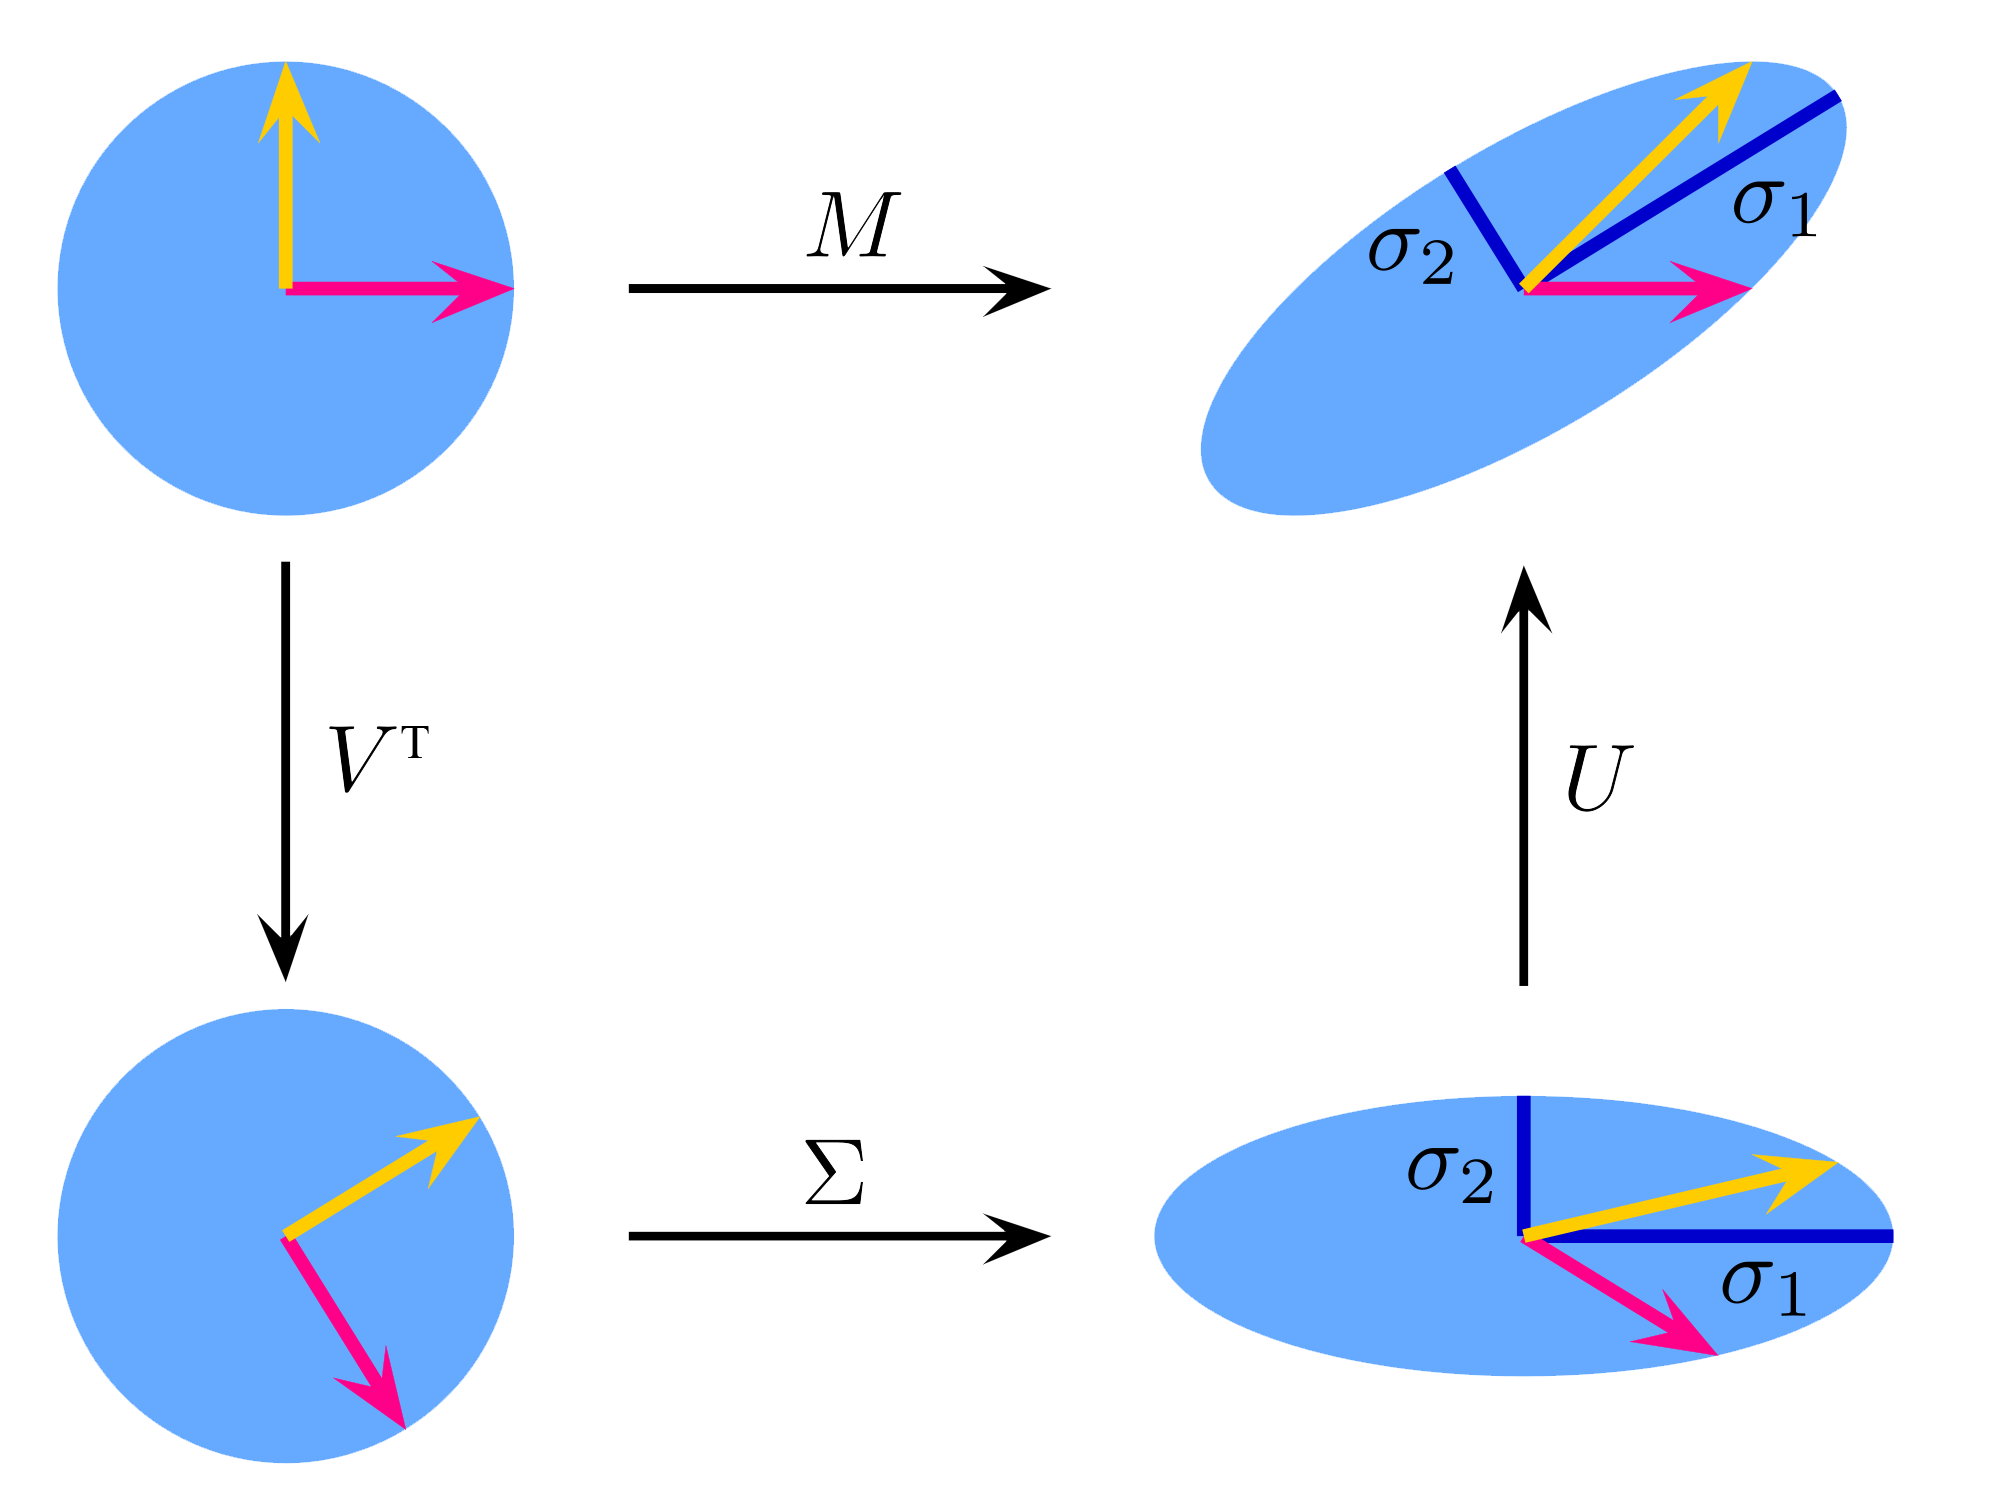
\includegraphics[width=0.65\textwidth]{Chapter7/images/image006.png} 
    \end{center}
\end{frame}




\begin{frame}\frametitle{A Procedure for Constructing the SVD of $A$}
    Suppose $A$ is $m \times n$ and has rank $r$. 
    
    \begin{enumerate}
        \item<2-> Compute the squared singular values of $A^TA$, $\sigma_i^2$, and construct $\Sigma$. \vspace{6pt}
        \item<3-> Compute the unit singular vectors of $A^TA$, $\vec v_i$, use them to form $V$. \vspace{6pt}
        \item<4-> Compute an orthonormal basis for Col$A$ using $$\vec u_i = \frac{1}{\sigma_i}A\vec v_i, \quad i = 1, 2, \ldots r$$ If necessary, extend the set $\{\vec u_i\}$ to form an orthonormal basis for $\mathbb R^m$ and use the basis to form $U$. 
    \end{enumerate}
\end{frame}




\begin{frame}\frametitle{Example}
    Construct the singular value decomposition for $A = 
    \begin{pmatrix}
    2 & 0 \\ 0 & -3 \\ 0 & 0 \\ 0 & 0 
    \end{pmatrix}
    $.
    
    \vspace{12pt}
    \pause 
    \Emph{Solution}\\ \pause 
    Singular values: 
    $$A^TA = \spalignmat{4 0;0 9} \quad \Rightarrow \quad \lambda_1 = 9, \lambda_2=4$$ \pause 
    The positive square roots of the eigenvalues are the singular values. 
    $$\sigma_1 = 3, \ \sigma_2 = 2$$
    \textit{Don't forget that $\sigma_1$ is the largest singular value.}
    
\end{frame}




\begin{frame}\frametitle{Example: Construct $\Sigma$ and $V$}    
    Using the singular values we can construct $\Sigma$. 
    $$\sigma_1 = 3, \ \sigma_2 = 2 \ \Rightarrow \ \Sigma = \spalignmat{3 0;0 2;0 0;0 0}$$
    
    \onslide<2->{Next we construct the right-singular vectors $\{\vec v_i\}$ and form $V$. }
    \begin{align*}
        \onslide<3->{A^TA - \lambda_1 I &= \spalignmat{-5 0;0 0} \quad \Rightarrow \quad \vec v_1 = \spalignmat{0;1}} \\
        \onslide<4->{A^TA - \lambda_2 I &= \spalignmat{-5 0;0 0} \quad \Rightarrow \quad \vec v_2 = \spalignmat{1;0} } \onslide<5->{\quad \Rightarrow \quad
        V = \spalignmat{\vec v_1  \vec v_2} = \spalignmat{0 1;1 0}}
    \end{align*}
\end{frame}




\begin{frame}\frametitle{Example: Construct $\vec u_i$}    
    Next we construct left-singular vectors $\{\vec u_i \}$ using $\vec u_i = \frac{1}{\sigma_i}A\vec v_i$ for $i = 1, 2, \ldots r$. \onslide<2->{Each $\vec u_i$ will be a unit vector in $\mathbb R^4$.}
    \begin{align*}
        \onslide<3->{\vec u_1 &= \frac{1}{\sigma_1}A\vec v_1 = \frac{1}{3}\begin{pmatrix}
    2 & 0 \\ 0 & -3 \\ 0 & 0 \\ 0 & 0 
    \end{pmatrix}\spalignmat{0;1} = \spalignmat{0;-1;0;0}}\\[12pt]
    \onslide<4->{\vec u_2 &= \frac{1}{\sigma_2}A\vec v_2 = \frac{1}{2}\begin{pmatrix}
    2 & 0 \\ 0 & -3 \\ 0 & 0 \\ 0 & 0 
    \end{pmatrix}\spalignmat{1;0} = \spalignmat{1;0;0;0}}
    \end{align*}

\end{frame}




\begin{frame}\frametitle{Example: Construct $U$}  

    To construct the SVD of $A$, we must construct the last two columns of $U$. 
    \begin{itemize}
        \item<2-> In this example, $A$ has rank $r=2$ and $U$ will be a $4 \times 4$ orthogonal matrix.
        \item<3-> Because the columns of $U$ must be orthonormal, and $\vec u_1$ and $\vec u_2$ were standard vectors, by inspection we can set the last two columns to be
        $$\vec u_3 = \spalignmat{0;0;1;0}, \quad \vec u_4 = \spalignmat{0;0;0;1}$$  
        Note that $\vec u_3$ and $\vec u_4$ are unit vectors, and that $\{\vec u_i\}$ are orthonormal. 
        \item<4-> We could have chosen other vectors for $\vec u_3$ and $\vec u_4$.
    \end{itemize}
    
\end{frame}




\begin{frame}\frametitle{Example: Construct $SVD$}  

    We have the SVD of $A$. 
    
    $$A = \begin{pmatrix}
    2 & 0 \\ 0 & -3 \\ 0 & 0 \\ 0 & 0 
    \end{pmatrix}
    = 
    \spalignmat{0 1 0 0;-1 0 0 0;0 0 1 0;0 0 0 1}
    \spalignmat{3 0;0 2;0 0;0 0}
    \spalignmat{0 1;1 0}
    $$
    
\end{frame}







\frame{\frametitle{Summary}

    \SummaryLine \vspace{4pt}
    \begin{itemize}\setlength{\itemsep}{8pt}

        \item the definition of the SVD
        \item computing the SVD for a matrix

    \end{itemize}
    
    \vspace{6pt}
}




    
    % \title{The SVD of a $3\times2$ Matrix with Rank 1}
\subtitle{\SubTitleName}
\institute[]{\Course}
\author{\Instructor}
\maketitle   


\frame{\frametitle{Topics and Objectives}
\Emph{Topics} \\
%\TopicStatement
\begin{itemize}

    \item the Singular Value Decomposition (SVD) of a matrix and how to compute the SVD for a given matrix % and some of its applications

\end{itemize}

\vspace{0.5cm}

\Emph{Learning Objectives}\\

%\LearningObjectiveStatement

\begin{itemize}

    \item compute the SVD for a rectangular matrix
    % \item Apply the SVD to 
    % \begin{itemize} 
    %     \item estimate the rank and condition number of a matrix, 
    %     \item construct a basis for the four fundamental spaces of a matrix, and
    %     \item construct a spectral decomposition of a matrix.
    % \end{itemize}
\end{itemize}

} 

\begin{frame}\frametitle{A Procedure for Constructing the SVD of $A$}
    Suppose $A$ is $m \times n$ and has rank $r$. 
    
    \begin{enumerate}
        \item<2-> Compute the squared singular values of $A^TA$, $\sigma_i^2$, and construct $\Sigma$. \vspace{6pt}
        \item<3-> Compute the unit singular vectors of $A^TA$, $\vec v_i$, use them to form $V$. \vspace{6pt}
        \item<4-> Compute an orthonormal basis for Col$A$ using $$\vec u_i = \frac{1}{\sigma_i}A\vec v_i, \quad i = 1, 2, \ldots r$$ If necessary, extend the set $\{\vec u_i\}$ to form an orthonormal basis for $\mathbb R^m$ and use the basis to form $U$. 
    
    \end{enumerate}
\end{frame}



\begin{frame}\frametitle{A $3\times2$ Matrix with Rank 1}
Construct the singular value decomposition of $ A = \begin{pmatrix}
1 & -1 \\ -2 & 2 \\ 2 & -2 
\end{pmatrix}$.  

    
    \Emph{Solution}\\
    Singular values: \onslide<3->{
    $$A^TA = \spalignmat{9 -9;-9 9} \quad \Rightarrow \quad \lambda_1 = 18, \ \lambda_2=0 \quad \Rightarrow \quad  \sigma_1 = \sqrt{18}, \ \sigma_2 = 0$$}
    \onslide<4->{Don't forget that }
    \begin{itemize}
        \item<4-> Singular matrices have eigenvalue 0 and the trace of a matrix is the sum of its eigenvalues. 
        \item<5-> The positive square roots of the eigenvalues are the singular values. 
        \item<6-> $\sigma_1$ is the largest singular value.
    \end{itemize}

    
\end{frame}




\begin{frame}\frametitle{Example: Construct $\Sigma$ and $V$}    

    Using the singular values we can construct $\Sigma$. 
    $$\sigma_1 = \sqrt{18} = 3\sqrt{2}, \quad \sigma_2 = 0 \qquad \Rightarrow \qquad \Sigma = \spalignmat{3\sqrt{2} 0;0 0;0 0}$$
    
    \onslide<2->{Next we construct the right-singular vectors $\{\vec v_i\}$ and form $V$. }
    \begin{align*}
        \onslide<3->{A^TA - \lambda_1 I &= \spalignmat{-9 -9;-9 -9} \quad \Rightarrow \quad \vec v_1 = \frac{1}{\sqrt{2}} \spalignmat{1;-1}} \\
        \onslide<4->{A^TA - \lambda_2 I &= \spalignmat{9 -9;-9 9} \quad \Rightarrow \quad \vec v_2 = \frac{1}{\sqrt{2}} \spalignmat{1;1} } \onslide<5->{\quad \Rightarrow \quad
        V  = \frac{1}{\sqrt2}\spalignmat{1 1;-1 1}}
    \end{align*}
\end{frame}




\begin{frame}\frametitle{Construct $\vec u_1$}    
    Next we construct left-singular vectors $\{\vec u_i \}$. The rank of $A$ is $r=1$, so we may use $$\vec u_i = \frac{1}{\sigma_i}A\vec v_i$$ for $i = 1$. \onslide<2->{Vector $\vec u_1$ will be a unit vector in $\mathbb R^3$.}
    \begin{align*}
        \onslide<3->{\vec u_1 = \frac{1}{\sigma_1}A\vec v_1 &= \frac{1}{3\sqrt2}
        \begin{pmatrix}
            1 & -1 \\ -2 & 2 \\ 2 & -2 
        \end{pmatrix}
        \spalignmat{1/\sqrt2;-1/\sqrt2} }\\
        \onslide<4->{&=\frac{1}{3\cdot2}\spalignmat{2;-4;4} = \frac{1}{3} \spalignmat{1;-2;2}}
    \end{align*}
    
\end{frame}




\begin{frame}\frametitle{Constructing $U$}  

    How can we construct the remaining left-singular vectors to construct $U$? 
    \begin{itemize}
        \item<2-> In this example, $A$ has rank $r=1$, and $U$ will be a $3 \times 3$ orthogonal matrix.
        \item<3-> By inspection, two vectors orthogonal to $\vec u_1$ are
        $$\vec x_2 = \spalignmat{2;1;0}, \quad \vec x_3 = \spalignmat{-2;0;1}, \quad \text{recall: } \vec u_1 = \frac{1}{3} \spalignmat{1;-2;2}$$
        \item<4-> Because $\vec u _1 \in \Col A$, these two vectors are in $(\Col A)\Perp$. 
        \item<5-> But $U$ is an orthogonal matrix, so how might we create an orthogonal basis for $(\Col A)\Perp$? 
    \end{itemize}
\end{frame}




\begin{frame}\frametitle{Constructing $U$}  

    Gram-Schmidt. 
    \begin{align*}
        \bar u_2 &= \vec x_2 = \spalignmat{2;1;0}\\
        \bar u_3 &= \vec x_3 - \frac{\vec x_3 \cdot \bar u_2 }{\bar u_2 \cdot \bar u_2}\bar u_2 = \spalignmat{-2;0;1} - \frac{-4}{5}\spalignmat{-2;0;1} = \frac 15 \spalignmat{-2;4;-5}
    \end{align*}
    Normalizing these vectors yields the remaining left singular vectors. 
    \begin{align*}
        \vec u_2 = \frac{1}{\sqrt 5} \spalignmat{2;1;0}, \quad \vec u_3 = \frac{1}{\sqrt{45}}\spalignmat{-2;4;-5}
    \end{align*}
\end{frame}




\begin{frame}\frametitle{Example: Construct $SVD$}  

    Thus, $A = U\Sigma V^T$, where
    \begin{align*}
        U &= \spalignmat{1/3 2/\sqrt5 -2/\sqrt{45};-2/3 1/\sqrt5 4/\sqrt{45}; 2/3 0 -5/\sqrt{45}}\\[4pt]
    \Sigma &= \spalignmat{3\sqrt2 0;0 0;0 0} \\[4pt]
    V &= \frac{1}{\sqrt2}\spalignmat{1 1;-1 1} 
    \end{align*} 
    
    
\end{frame}



\frame{\frametitle{Summary}

    \SummaryLine \vspace{4pt}
    \begin{itemize}\setlength{\itemsep}{8pt}

        % \item the definition of the SVD
        \item computing the SVD for a matrix
        \item applying Gram-Schmidt to construct the SVD of a matrix % form an orthonormal basis for $\mathbb R^m$

    \end{itemize}
    
    \vspace{6pt}
    
    \pause 
}




       
% \fi

% \ifnum \Week = 15    
%      \newcommand{\SubTitleName}{Symmetric Matrices and the SVD} 

    % \title{The SVD and the Condition Number of a Matrix}
\subtitle{\SubTitleName}
\institute[]{\Course}
\author{\Instructor}
\maketitle   


\frame{\frametitle{Topics and Objectives}
\Emph{Topics} \\
%\TopicStatement
\begin{itemize}

    \item the Singular Value Decomposition (SVD) of a matrix and the condition number of a matrix

\end{itemize}

\vspace{0.5cm}

\Emph{Learning Objectives}\\

%\LearningObjectiveStatement

\begin{itemize}

    % \item compute the SVD for a rectangular matrix
    \item apply the SVD to estimate the rank and condition number of a matrix
    %     \item construct a basis for the four fundamental spaces of a matrix, and
    %     \item construct a spectral decomposition of a matrix.
    % \end{itemize}
\end{itemize}

} 

\begin{frame} \frametitle{Applications of the SVD}

    The SVD has been applied to many modern applications in CS, engineering, and mathematics. % (our textbook mentions the first four).
    
    \begin{small}
    \begin{itemize}
        \item estimating the rank and condition number of a matrix
        \item constructing bases for the four fundamental spaces
        \item computing the pseudoinverse of a matrix
        \item linear least squares problems
        % \item Non-linear least-squares  https://en.wikipedia.org/wiki/Non-linear\_least\_squares        
        \item machine learning and data mining % \\ https://en.wikipedia.org/wiki/K-SVD
        \item facial recognition % \\ https://en.wikipedia.org/wiki/Eigenface
        \item principle component analysis % \\ https://en.wikipedia.org/wiki/Principal\_component\_analysis
        \item image compression
    \end{itemize}
    \end{small}
    
    % \textit{Students are expected to be familiar with the 1$^{st}$ two items in the list}. 
 
\end{frame}

\begin{frame} \frametitle{The Condition Number of a Matrix}

    If $A$ is an invertible $n\times n$ matrix, the ratio $$\frac{\sigma_1}{\sigma_n}$$ is the \Emph{condition number} of $A$.

    \vspace{12pt} 
    \Emph{Example}: Suppose $A = \spalignmat{2 -1;2 1}$. We found that $\sigma_1 = \sqrt8, \sigma_2 = \sqrt2$. \pause Therefore, the condition number of $A$ is
    
    $$\frac{\sigma_1}{\sigma_n} = \frac{\sqrt8}{\sqrt2}=2$$
    
\end{frame}

\begin{frame} \frametitle{Notes on the Condition Number}


        \begin{itemize}
        \item<2-> In some applications of linear algebra, entries of $A$ and contain errors. The condition number of a matrix describes the sensitivity that any approach to determining solutions to $A\vec x = \vec b$ might have to errors in $A$.
        \item<3-> The larger the condition number, the more sensitive the system is to errors. 
        \item<4-> We could define the condition number for a rectangular matrix, but that would go beyond the scope of this course.
    \end{itemize}

\end{frame}




\frame{\frametitle{Summary}

    \SummaryLine \vspace{4pt}
    \begin{itemize}\setlength{\itemsep}{8pt}

        \item applying the SVD to compute the condition number of a matrix

    \end{itemize}
    
    \vspace{6pt}
}



    
    % \title{The SVD and the Spectral Decomposition of a Matrix}
\subtitle{\SubTitleName}
\institute[]{\Course}
\author{\Instructor}
\maketitle   


\frame{\frametitle{Topics and Objectives}
\Emph{Topics} \\
%\TopicStatement
\begin{itemize}

    \item the Singular Value Decomposition (SVD) of a matrix and the spectral decomposition

\end{itemize}

\vspace{0.5cm}

\Emph{Learning Objectives}\\

%\LearningObjectiveStatement

\begin{itemize}

    % \item compute the SVD for a rectangular matrix
    \item apply the SVD to construct a spectral decomposition of a matrix
    % \end{itemize}
\end{itemize}

} 

\begin{frame}\frametitle{Motivation: Approximation}

    Recall that from calculus, Taylor expansions and Taylor polynomials, can be used to approximate functions near a point.
    \pause 
    \begin{center}
    \begin{tikzpicture}[domain=-8:7] 
        \begin{axis}[
        width=4in,
        height=2.0in,
        grid=both,
        grid style={line width=.2pt, draw=gray!30},
        clip=false,
        axis lines=middle,
        xmin=-7.1,xmax=7.1,
        ymin=-2.1,ymax=2.1,
        restrict y to domain=-2:4,
        xtick={-6.28,-3.14,0,3.14,6.28},
        xticklabels={, , , , , , , , , ,},
        ytick={-2,-1,0,1,2},
        yticklabels={, , , , , , , , , ,},
        extra x ticks={-6.28,-3.14,0,3.14,6.28},
        extra y ticks={1},
        extra x tick style={xticklabel style={fill=white, circle, inner sep=1.5pt}},
        extra y tick style={xticklabel style={fill=white, circle, inner sep=1.5pt}},
        extra x tick labels={$-2\pi$, $-\pi$,$0$, $\pi$,$2\pi$},
        extra y tick labels={1},
        axis line style={shorten >=-7.5pt, shorten <=-7.5pt},
        xlabel=$x$,
        ylabel=$y$,
        xlabel style={at={(ticklabel* cs:1)},anchor=north west},
        ylabel style={at={(ticklabel* cs:1)},anchor=south east}
        ]
        
        \addplot[samples=100,domain=-7:7,smooth, thick] {sin(deg(x))} node[pos=1] (endofplotsquare) {};
        \node [right] at (endofplotsquare) {$\sin(x)$};  
        
        \addplot[samples=100,domain=-2:2,smooth, very thick,DarkRed] {x} node[pos=1] (endofplotsquare) {};
        \node [right] at (endofplotsquare) {$p_1(x)=x$};
        
        \addplot[samples=100,domain=-3.1:3.1,smooth, very thick,DarkBlue] {x-x*x*x/6} node[pos=1] (endofplotsquare) {};
        \node [right] at (endofplotsquare) {$p_3(x)=x-x^3/6$};           
        \end{axis}

    \end{tikzpicture}   
    \end{center}
    \pause Students are not expected to be familiar with Taylor expansions in this course, but, can we use expansions to approximate matrices? 
\end{frame}


\begin{frame}\frametitle{Recall: Spectral Decomposition of a Symmetric Matrix}

    \begin{center}\begin{tikzpicture} \node [mybox](box){\begin{minipage}{0.75\textwidth}\vspace{4pt}
        Suppose $A$ can be orthogonally diagonalized as 
        \begin{equation*}
        A = P D P ^{T} = \begin{pmatrix}
        \vec u_1 & \cdots & \vec u_n 
        \end{pmatrix}
        \begin{pmatrix}
            \lambda _1 & \cdots & 0 
            \\
            \vdots & \ddots &  \vdots
            \\
            0 & \cdots & \lambda _n 
        \end{pmatrix}
        \begin{pmatrix}
            \vec u_1  ^{T}  \\ \vdots \\ \vec u_n  ^{T} 
        \end{pmatrix}
        \end{equation*}
        Then $A$ has the decomposition
        $$A = 
        \lambda _1 \vec u_1 \vec u_1 ^{T}  + \cdots + \lambda _n \vec u_n \vec u_n ^{T} 
        = \sum_{i=1}^{n} \lambda_i \vec u_i \vec u_i^T$$
        \end{minipage}};
    \node[fancytitle, right=10pt] at (box.north west) {Spectral Decomposition};
    \end{tikzpicture}\end{center}
    
    \pause 
    
    Can we give a more general result using the SVD? 

    
\end{frame}

\begin{frame} \frametitle{The Spectral Decomposition of a Matrix Using SVD}

    The SVD can also be used to construct the spectral decomposition for any matrix with rank $r$.
    \begin{equation*}
        A = \sum_{i=1} ^{r} \sigma _i \vec u _{i} \vec v _{i}\, ^{T}
    \end{equation*}
    Vectors $ \vec u_i, \vec v_i$ are the $ i^{th}$ columns of $ U$ and $ V$ respectively. \begin{itemize}\setlength{\itemsep}{4pt}
        \item<2-> The proof similar to the proof we used for the symmetric case. 
        \item<3-> Each term in this sum is a rank 1 matrix. 
        \item<4-> In applications of linear algebra, $\sigma_i$ can become sufficiently small, allowing us to approximate $A$ with a small number of rank 1 matrices. 
        \item<5-> For the case when $A=A^T$, we obtain the same spectral decomposition obtained using the orthogonal diagonalization of $A$, or $A=PDP^T$. 
    \end{itemize}
    
\end{frame}


\begin{frame}\frametitle{Example}
    Suppose $A$ has the following SVD. {\small
    $$A = \begin{pmatrix}
    2 & 0 \\ 0 & -3 \\ 0 & 0 \\ 0 & 0 
    \end{pmatrix}
    = 
    \spalignmat{0 1 0 0;-1 0 0 0;0 0 1 0;0 0 0 1}
    \spalignmat{3 0;0 2;0 0;0 0}
    \spalignmat{0 1;1 0}
    $$
    }
    \onslide<2->{The spectral decomposition of $A$ is as follows.} {\small
    \begin{align*}
        \onslide<3->{A &= \sum_{s=1} ^{r} \sigma _s \vec u _{s} \vec v _{s} ^{T} }
        \onslide<4->{= 3 \spalignmat{0;-1;0;0}\spalignmat{0 1} + 2\spalignmat{1;0;0;0}\spalignmat{1 0} }\onslide<5->{= 3 \spalignmat{0 0;0 -1;0 0;0 0} + 2\spalignmat{1 0;0 0;0 0;0 0}}
    \end{align*}
    }
\end{frame}
    

\frame{\frametitle{Summary}

    \SummaryLine \vspace{4pt}
    \begin{itemize}\setlength{\itemsep}{8pt}

        \item applying the SVD to construct a spectral decomposition of a matrix

    \end{itemize}
    
    \vspace{6pt}
    \pause 
}


% \frame{\frametitle{Understanding Relationships Between Ideas}

% \textit{"At the end of eleventh grade, I took the measure of the situation, and came to the conclusion that rapidity does not have a precise relation to intelligence. What is important is to deeply understand things and their relations to each other ... the fact of being quick or slow is not really relevant” \\ - Laurent Schwartz, Field’s Medal Winning Mathematician." } \\ \vspace{12pt}
% \pause 
%  You may find that the material in this section, or perhaps in other parts of the course, takes longer than expected to learn. This is normal.   

    
% }

    
    % 
\title{The SVD and the Four Fundamental Subspaces}
\subtitle{\SubTitleName}
\institute[]{\Course}
\author{\Instructor}
\maketitle   


\frame{\frametitle{Topics and Objectives}
\Emph{Topics} \\
%\TopicStatement
\begin{itemize}

    \item the Singular Value Decomposition (SVD) of a matrix and the four fundamental subspaces

\end{itemize}

\vspace{0.5cm}

\Emph{Learning Objectives}\\

%\LearningObjectiveStatement

\begin{itemize}

    % \item compute the SVD for a rectangular matrix
    \item apply the SVD to construct bases for the four fundamental subspaces of a matrix
    %     \item construct a spectral decomposition of a matrix.
    % \end{itemize}
\end{itemize}

} 

\begin{frame}{The Four Fundamental Subspaces of a Matrix}



    % The idea behind this theorem is described in the diagram below. 
    \pause 
    
    \begin{center}
    \begin{tikzpicture}[scale=.85]
        
        \onslide<2->{
        % boxes
        \filldraw[draw=DarkBlue!50,fill=DarkBlue!15] (0,0) -- (-1,1) -- (1,3) -- (2,2) -- cycle;
        \filldraw[draw=DarkBlue!50,fill=DarkBlue!15] (0,0) -- (1,-1) -- (0,-2) -- (-1,-1) -- cycle;      
        \draw (0.4, 1.7) node[below]{\small $\Row A$};
        \draw (0.0,-0.7) node[below]{\small $\Nul A$};        
        }
        
        \onslide<3->
        {
        \filldraw[draw=DarkGreen!50,fill=DarkGreen!15] (4,0) -- (2.5, 1.5) -- (3.5, 2.5) -- (5,1) -- cycle;
        \filldraw[draw=DarkGreen!50,fill=DarkGreen!15] (4,0) -- (5.5,-1.5) -- (4.5,-2.5) -- (3,-1) -- cycle;        
        \draw (3.9, 1.5) node[below]{\small $\Col A$};
        \draw (4.2, -0.8) node[below]{\small $\Nul A^T$};        
        }

        \onslide<4->{
        \draw (-1.0,0.5) node[below]{\Large $\color{DarkBlue} \mathbb R^n$};
        }

        \onslide<5->{
        \draw ( 5.2,0.5) node[below]{\Large $\color{DarkGreen} \mathbb R^m$};
        }
        
    \end{tikzpicture}\
    
    \vspace{12pt}
    \pause 
    The SVD of $A$ can be used construct bases for these subspaces. 
        
    \end{center}

\end{frame}

\begin{frame}{Recall: the SVD and the Four Fundamental Spaces}

Suppose $\vec v_i$ are orthonormal eigenvectors for $A^TA$, and $$\vec u _i = \frac{1}{\sigma_i}A\vec v_ i \ \text{ for } i \le r = \Rank A, \ \sigma_i = \lVert A \vec v_i \rVert.$$ Then we have the following bases for any $m\times n$ real matrix $A$. 
\begin{itemize}

    \item<2->  $ \vec v_1 ,\dotsc, \vec v_r$ is an orthonormal basis for $ \textup{Row} A$. 
    
    \item<2->  $ \vec v_{r+1} ,\dotsc, \vec v_n$ is an orthonormal basis for $ \Nul  A $. 
    
    
    \item<3->  $ \vec u_1 ,\dotsc, \vec u_r$ is an orthonormal basis for $ \textup{Col} A$.  
    
\end{itemize}

\vspace{12pt}

\onslide<4->{We can now also see that because $U$ is an orthogonal matrix, $ \vec u_{r+1} ,\dotsc, \vec u_m$ give an orthonormal basis for $ \Nul  A ^{T}$. }

\end{frame}


\begin{frame}\frametitle{Example}
    Given the SVD of $A$, determine $\text{rank}(A)$, and bases for $\Nul A$ and for $\Col A$.
    % \vspace{6pt} 
    \begin{align*}
        A = U \Sigma V^T = \spalignmat{0 1 0 0;0 0 1 0;0 0 0 -1;-1 0 0 0} \spalignmat{5 0 0 0 0;0 3 0 0 0;0 0 2 0 0;0 0 0 0 0} \spalignmat{0 0 \sqrt{0.8} 0 -\sqrt{0.2}; 1 0 0 0 0;0 1 0 0 0;0 0 0 1 0;0 0 \sqrt{0.8} 0 \sqrt{0.2}}
    \end{align*}

    \onslide<2->{\Emph{Solution} }
    \begin{itemize}
        \item<3-> there are exactly three non-zero singular values $\Rightarrow$ rank$A = 3$
        \item<4-> the last two columns of $V$ (or rows of $V^T$) are a basis for $\Nul A$
        \item<5-> first three columns of $U$ are a basis for $\Col A$
    \end{itemize}

\end{frame}


% \begin{frame} \frametitle{Example Solution}


% \end{frame}








\frame{\frametitle{Summary}

    \SummaryLine \vspace{4pt}
    \begin{itemize}\setlength{\itemsep}{8pt}

        \item applying the SVD to construct a bases for the four fundamental subspaces of a matrix

    \end{itemize}
    
    \vspace{6pt}
    \pause 
}



    % REDO

% \fi

% \ifnum \Week = 20  
%     





%% FRAME
\begin{frame} \frametitle{MATH 2552: Canvas Tour}

\begin{enumerate}
    \item Syllabus
    \item Announcements
    \item Lecture videos
    \item Piazza
    \item Written Assignments
    \item Lecture Slides
    \item Studio Worksheets
    \item Webwork
    \item Midterm Procedures
    \item Textbook
\end{enumerate}


\end{frame}

% \fi



% \input{Chapter7/7_1}
% \input{Chapter7/7_2}
% \input{Chapter7/7_3}
% \input{Chapter7/7_4}
\fi
\ifnum \AspectRatio=2
\title{Basic and Free Variables} 
\subtitle{\SubTitleName}
\institute[]{\Course}
\author{\Instructor}
\maketitle   




\frame{\frametitle{Topics and Learning Objectives}
\Emph{Topics} \\
\TopicStatement


\begin{itemize}
    % \item consistency, existence, uniqueness
    % \item row reduction algorithm
    \item pivots, and basic and free variables 
    %\item Parametrized solution sets 
    % \item Echelon forms, existence and uniqueness 
\end{itemize}

\vspace{0.5cm}

\LO\\

\LearningObjectiveStatement

\begin{itemize}
    \item Characterize a linear system in terms of the number of leading entries, \Emph{basic and free variables}, pivots, pivot columns, pivot positions.
    % \item determine whether a linear system is consistent from its echelon form
    % \item apply the row reduction algorithm to compute the coefficients of a polynomial
\end{itemize}

}



\frame{\frametitle{Basic and Free Variables}
\vspace{-22pt}
\begin{align*} \begin{amatrix}{1} A & \vec b \ \end{amatrix} = &
\begin{amatrix}{5}
1 & 0 & 0 & 7 & 2 & 4 
\\
0 & 0 & 1 & 4 & 4 & 5 
\\
0 & 0 & 0 & 0 & 2 & 4 
\end{amatrix}
\end{align*}
Leading entries are in first, third, and fifth columns.
\begin{itemize}
    \item<2->\Emph{Pivot columns}: in the first, third, and fifth columns
    \item<3-> Variables that correspond to pivots are $x_1$, $x_3$, and $x_5$. 
    \item<4-> Variables that correspond to a pivot are \Emph{basic variables}.
    \item<4-> Variables that are not basic are \Emph{free variables}. They can take any value. 
    \item<5-> The free variables are $x_2$ and $x_4$. Any choice of the free variables leads to a solution of the system.  
\end{itemize}
\vspace{4pt}
}



\frame{\frametitle{Notes on Basic and Free Variables}


\begin{itemize}
    \item <1-> Note that a matrix, on its own, does not have basic variables or free variables. Systems have variables. 
    \item <2-> If $A$ has $n$ columns, then the linear system $$\begin{amatrix}{1} A & \vec b \ \end{amatrix}$$ must have $n$ variables. One variable for each column of the matrix. 
    \item <3-> There are two types of variables: basic and free. And a variable cannot be both free and basic at the same time. 
    \begin{align*}
    n 
    &= \text{number of columns of } A \\
    &= (\text{number of basic variables}) + (\text{number of free variables}) 
    \end{align*}
\end{itemize}

}




\frame{\frametitle{Existence and Uniqueness}

\begin{center}\begin{tikzpicture} \node [mybox](box){\begin{minipage}{0.90\textwidth}\vspace{4pt}

A linear system is consistent if and only if (exactly when) the last column of the \Emph{augmented} matrix does not have a pivot. This is the same as saying that the RREF of the augmented matrix does \Emph{not} have a row of the form
$$\spalignmat{0 , 0, 0,  \cdots, 0 | 1}$$
Moreover, if a linear system is consistent, then it has
\begin{enumerate}
    \item a unique solution if and only if there are no free variables, and
    \item infinitely many solutions that are parameterized by free variables. 
\end{enumerate}
\end{minipage}};
\node[fancytitle, right=10pt] at (box.north west) {Theorem};
\end{tikzpicture}\end{center}

}




\frame{\frametitle{Example: Existence and Uniqueness}

    If possible, determine the coefficients of the polynomial $y(t) = a_0t+a_1t^2$ that passes through the points that are given in the form $(t,y)$. 
    \begin{enumerate}[a)]\setlength{\itemsep}{12pt}
        \item $L(-1,0)$ and $M(1,1)$
        \item $P(2,0)$, $Q(1,1)$, and $R(0,2)$
    \end{enumerate}


}

\frame{\frametitle{Solution Approach: Problem a)}
    Let's convert this to a linear system:
    \begin{itemize}
        \item For point $L(-1,0)$: $-a_0 + a_1 = 0$
        \item For point $M(1,1)$: $a_0 + a_1 = 1$
    \end{itemize}
    The augmented matrix is:
    \[\left(\begin{array}{cc|c}
        -1 & 1 & 0 \\
        1 & 1 & 1
    \end{array}\right)\]
}

\frame{\frametitle{Row Reduction: Problem a)}
    Let's find the RREF:
    \[
    \begin{array}{rcl}
    & \left(\begin{array}{cc|c}
        -1 & 1 & 0 \\
        1 & 1 & 1
    \end{array}\right) &
    \\[1em]
    & \left(\begin{array}{cc|c}
        1 & -1 & 0 \\
        1 & 1 & 1
    \end{array}\right) & R_1 \rightarrow -R_1
    \\[1em]
    & \left(\begin{array}{cc|c}
        1 & -1 & 0 \\
        0 & 2 & 1
    \end{array}\right) & R_2 \rightarrow R_2 - R_1
    \\[1em]
    & \left(\begin{array}{cc|c}
        1 & -1 & 0 \\
        0 & 1 & \frac{1}{2}
    \end{array}\right) & R_2 \rightarrow \frac{1}{2}R_2
    \\[1em]
    & \left(\begin{array}{cc|c}
        1 & 0 & \frac{1}{2} \\
        0 & 1 & \frac{1}{2}
    \end{array}\right) & R_1 \rightarrow R_1 + R_2
    \end{array}
    \]
}

\frame{\frametitle{Analysis of Basic and Free Variables: Problem a)}
    From the RREF:
    \begin{itemize}
        \item Pivot columns are 1 and 2 (corresponding to $a_0$ and $a_1$)
        \item All variables are basic variables (no free variables)
        \item The last column has no pivot
        \item Therefore:
            \begin{itemize}
                \item The system is consistent (no row of zeros with nonzero constant)
                \item The solution is unique (no free variables)
            \end{itemize}
        \item Solution: $a_0 = \frac{1}{2}$, $a_1 = \frac{1}{2}$
    \end{itemize}
}

\frame{\frametitle{Solution Approach: Problem b)}
    For three points, we get:
    \begin{itemize}
        \item $P(2,0)$: $2a_0 + 4a_1 = 0$
        \item $Q(1,1)$: $a_0 + a_1 = 1$
        \item $R(0,2)$: $0 = 2$
    \end{itemize}
    The augmented matrix is:
    \[\left(\begin{array}{cc|c}
        2 & 4 & 0 \\
        1 & 1 & 1 \\
        0 & 0 & 2
    \end{array}\right)\]
}

\frame{\frametitle{Row Reduction: Problem b)}
    Finding the RREF:
    \[\left(\begin{array}{cc|c}
        2 & 4 & 0 \\
        1 & 1 & 1 \\
        0 & 0 & 2
    \end{array}\right) \rightarrow
    \left(\begin{array}{cc|c}
        1 & 2 & 0 \\
        0 & -1 & 1 \\
        0 & 0 & 2
    \end{array}\right)\]
    Note the row $\begin{bmatrix} 0 & 0 & 2 \end{bmatrix}$
}

\frame{\frametitle{Analysis of Existence: Problem b)}
    Key observations:
    \begin{itemize}
        \item The RREF contains a row $\begin{bmatrix} 0 & 0 & 2 \end{bmatrix}$
        \item By the theorem, this means the system is inconsistent
        \item The inconsistency arises because:
            \begin{itemize}
                \item At $t=0$, any polynomial $a_0t + a_1t^2$ equals 0
                \item But point $R(0,2)$ requires $y(0)=2$
                \item This contradiction proves no solution exists
            \end{itemize}
    \end{itemize}
}

\frame{\frametitle{Connection to Theory}
    These examples illustrate key concepts.
    
    \pause 
    \textbf{Problem a)}
            \begin{itemize}
                \item Number of equations = number of variables
                \item All variables are basic (pivot columns)
                \item Unique solution exists
            \end{itemize}

            \pause 
    \textbf{Problem b)}
            \begin{itemize}
                \item More equations than variables (overdetermined)
                \item Last column has a pivot
                \item System is inconsistent
            \end{itemize}
}

\frame{\frametitle{Summary: Fundamental Questions}

In this video we explored the following concepts. \vspace{4pt}
\begin{itemize}\setlength{\itemsep}{8pt}
    \item augmented matrices and consistent systems
    \item pivots, and basic and free variables 
    \item fundamental questions that we will revisit throughout the course regarding consistency, existence, uniqueness
\end{itemize}

}


\fi

\end{document}